% Options for packages loaded elsewhere
\PassOptionsToPackage{unicode}{hyperref}
\PassOptionsToPackage{hyphens}{url}
\PassOptionsToPackage{dvipsnames,svgnames,x11names}{xcolor}
%
\documentclass[
  letterpaper,
  DIV=11,
  numbers=noendperiod]{scrreprt}

\usepackage{amsmath,amssymb}
\usepackage{lmodern}
\usepackage{iftex}
\ifPDFTeX
  \usepackage[T1]{fontenc}
  \usepackage[utf8]{inputenc}
  \usepackage{textcomp} % provide euro and other symbols
\else % if luatex or xetex
  \usepackage{unicode-math}
  \defaultfontfeatures{Scale=MatchLowercase}
  \defaultfontfeatures[\rmfamily]{Ligatures=TeX,Scale=1}
\fi
% Use upquote if available, for straight quotes in verbatim environments
\IfFileExists{upquote.sty}{\usepackage{upquote}}{}
\IfFileExists{microtype.sty}{% use microtype if available
  \usepackage[]{microtype}
  \UseMicrotypeSet[protrusion]{basicmath} % disable protrusion for tt fonts
}{}
\makeatletter
\@ifundefined{KOMAClassName}{% if non-KOMA class
  \IfFileExists{parskip.sty}{%
    \usepackage{parskip}
  }{% else
    \setlength{\parindent}{0pt}
    \setlength{\parskip}{6pt plus 2pt minus 1pt}}
}{% if KOMA class
  \KOMAoptions{parskip=half}}
\makeatother
\usepackage{xcolor}
\setlength{\emergencystretch}{3em} % prevent overfull lines
\setcounter{secnumdepth}{5}
% Make \paragraph and \subparagraph free-standing
\ifx\paragraph\undefined\else
  \let\oldparagraph\paragraph
  \renewcommand{\paragraph}[1]{\oldparagraph{#1}\mbox{}}
\fi
\ifx\subparagraph\undefined\else
  \let\oldsubparagraph\subparagraph
  \renewcommand{\subparagraph}[1]{\oldsubparagraph{#1}\mbox{}}
\fi

\usepackage{color}
\usepackage{fancyvrb}
\newcommand{\VerbBar}{|}
\newcommand{\VERB}{\Verb[commandchars=\\\{\}]}
\DefineVerbatimEnvironment{Highlighting}{Verbatim}{commandchars=\\\{\}}
% Add ',fontsize=\small' for more characters per line
\usepackage{framed}
\definecolor{shadecolor}{RGB}{241,243,245}
\newenvironment{Shaded}{\begin{snugshade}}{\end{snugshade}}
\newcommand{\AlertTok}[1]{\textcolor[rgb]{0.68,0.00,0.00}{#1}}
\newcommand{\AnnotationTok}[1]{\textcolor[rgb]{0.37,0.37,0.37}{#1}}
\newcommand{\AttributeTok}[1]{\textcolor[rgb]{0.40,0.45,0.13}{#1}}
\newcommand{\BaseNTok}[1]{\textcolor[rgb]{0.68,0.00,0.00}{#1}}
\newcommand{\BuiltInTok}[1]{\textcolor[rgb]{0.00,0.23,0.31}{#1}}
\newcommand{\CharTok}[1]{\textcolor[rgb]{0.13,0.47,0.30}{#1}}
\newcommand{\CommentTok}[1]{\textcolor[rgb]{0.37,0.37,0.37}{#1}}
\newcommand{\CommentVarTok}[1]{\textcolor[rgb]{0.37,0.37,0.37}{\textit{#1}}}
\newcommand{\ConstantTok}[1]{\textcolor[rgb]{0.56,0.35,0.01}{#1}}
\newcommand{\ControlFlowTok}[1]{\textcolor[rgb]{0.00,0.23,0.31}{#1}}
\newcommand{\DataTypeTok}[1]{\textcolor[rgb]{0.68,0.00,0.00}{#1}}
\newcommand{\DecValTok}[1]{\textcolor[rgb]{0.68,0.00,0.00}{#1}}
\newcommand{\DocumentationTok}[1]{\textcolor[rgb]{0.37,0.37,0.37}{\textit{#1}}}
\newcommand{\ErrorTok}[1]{\textcolor[rgb]{0.68,0.00,0.00}{#1}}
\newcommand{\ExtensionTok}[1]{\textcolor[rgb]{0.00,0.23,0.31}{#1}}
\newcommand{\FloatTok}[1]{\textcolor[rgb]{0.68,0.00,0.00}{#1}}
\newcommand{\FunctionTok}[1]{\textcolor[rgb]{0.28,0.35,0.67}{#1}}
\newcommand{\ImportTok}[1]{\textcolor[rgb]{0.00,0.46,0.62}{#1}}
\newcommand{\InformationTok}[1]{\textcolor[rgb]{0.37,0.37,0.37}{#1}}
\newcommand{\KeywordTok}[1]{\textcolor[rgb]{0.00,0.23,0.31}{#1}}
\newcommand{\NormalTok}[1]{\textcolor[rgb]{0.00,0.23,0.31}{#1}}
\newcommand{\OperatorTok}[1]{\textcolor[rgb]{0.37,0.37,0.37}{#1}}
\newcommand{\OtherTok}[1]{\textcolor[rgb]{0.00,0.23,0.31}{#1}}
\newcommand{\PreprocessorTok}[1]{\textcolor[rgb]{0.68,0.00,0.00}{#1}}
\newcommand{\RegionMarkerTok}[1]{\textcolor[rgb]{0.00,0.23,0.31}{#1}}
\newcommand{\SpecialCharTok}[1]{\textcolor[rgb]{0.37,0.37,0.37}{#1}}
\newcommand{\SpecialStringTok}[1]{\textcolor[rgb]{0.13,0.47,0.30}{#1}}
\newcommand{\StringTok}[1]{\textcolor[rgb]{0.13,0.47,0.30}{#1}}
\newcommand{\VariableTok}[1]{\textcolor[rgb]{0.07,0.07,0.07}{#1}}
\newcommand{\VerbatimStringTok}[1]{\textcolor[rgb]{0.13,0.47,0.30}{#1}}
\newcommand{\WarningTok}[1]{\textcolor[rgb]{0.37,0.37,0.37}{\textit{#1}}}

\providecommand{\tightlist}{%
  \setlength{\itemsep}{0pt}\setlength{\parskip}{0pt}}\usepackage{longtable,booktabs,array}
\usepackage{calc} % for calculating minipage widths
% Correct order of tables after \paragraph or \subparagraph
\usepackage{etoolbox}
\makeatletter
\patchcmd\longtable{\par}{\if@noskipsec\mbox{}\fi\par}{}{}
\makeatother
% Allow footnotes in longtable head/foot
\IfFileExists{footnotehyper.sty}{\usepackage{footnotehyper}}{\usepackage{footnote}}
\makesavenoteenv{longtable}
\usepackage{graphicx}
\makeatletter
\def\maxwidth{\ifdim\Gin@nat@width>\linewidth\linewidth\else\Gin@nat@width\fi}
\def\maxheight{\ifdim\Gin@nat@height>\textheight\textheight\else\Gin@nat@height\fi}
\makeatother
% Scale images if necessary, so that they will not overflow the page
% margins by default, and it is still possible to overwrite the defaults
% using explicit options in \includegraphics[width, height, ...]{}
\setkeys{Gin}{width=\maxwidth,height=\maxheight,keepaspectratio}
% Set default figure placement to htbp
\makeatletter
\def\fps@figure{htbp}
\makeatother
\newlength{\cslhangindent}
\setlength{\cslhangindent}{1.5em}
\newlength{\csllabelwidth}
\setlength{\csllabelwidth}{3em}
\newlength{\cslentryspacingunit} % times entry-spacing
\setlength{\cslentryspacingunit}{\parskip}
\newenvironment{CSLReferences}[2] % #1 hanging-ident, #2 entry spacing
 {% don't indent paragraphs
  \setlength{\parindent}{0pt}
  % turn on hanging indent if param 1 is 1
  \ifodd #1
  \let\oldpar\par
  \def\par{\hangindent=\cslhangindent\oldpar}
  \fi
  % set entry spacing
  \setlength{\parskip}{#2\cslentryspacingunit}
 }%
 {}
\usepackage{calc}
\newcommand{\CSLBlock}[1]{#1\hfill\break}
\newcommand{\CSLLeftMargin}[1]{\parbox[t]{\csllabelwidth}{#1}}
\newcommand{\CSLRightInline}[1]{\parbox[t]{\linewidth - \csllabelwidth}{#1}\break}
\newcommand{\CSLIndent}[1]{\hspace{\cslhangindent}#1}

\KOMAoption{captions}{tableheading}
\makeatletter
\@ifpackageloaded{tcolorbox}{}{\usepackage[many]{tcolorbox}}
\@ifpackageloaded{fontawesome5}{}{\usepackage{fontawesome5}}
\definecolor{quarto-callout-color}{HTML}{909090}
\definecolor{quarto-callout-note-color}{HTML}{0758E5}
\definecolor{quarto-callout-important-color}{HTML}{CC1914}
\definecolor{quarto-callout-warning-color}{HTML}{EB9113}
\definecolor{quarto-callout-tip-color}{HTML}{00A047}
\definecolor{quarto-callout-caution-color}{HTML}{FC5300}
\definecolor{quarto-callout-color-frame}{HTML}{acacac}
\definecolor{quarto-callout-note-color-frame}{HTML}{4582ec}
\definecolor{quarto-callout-important-color-frame}{HTML}{d9534f}
\definecolor{quarto-callout-warning-color-frame}{HTML}{f0ad4e}
\definecolor{quarto-callout-tip-color-frame}{HTML}{02b875}
\definecolor{quarto-callout-caution-color-frame}{HTML}{fd7e14}
\makeatother
\makeatletter
\makeatother
\makeatletter
\@ifpackageloaded{bookmark}{}{\usepackage{bookmark}}
\makeatother
\makeatletter
\@ifpackageloaded{caption}{}{\usepackage{caption}}
\AtBeginDocument{%
\ifdefined\contentsname
  \renewcommand*\contentsname{Table of contents}
\else
  \newcommand\contentsname{Table of contents}
\fi
\ifdefined\listfigurename
  \renewcommand*\listfigurename{List of Figures}
\else
  \newcommand\listfigurename{List of Figures}
\fi
\ifdefined\listtablename
  \renewcommand*\listtablename{List of Tables}
\else
  \newcommand\listtablename{List of Tables}
\fi
\ifdefined\figurename
  \renewcommand*\figurename{Figure}
\else
  \newcommand\figurename{Figure}
\fi
\ifdefined\tablename
  \renewcommand*\tablename{Table}
\else
  \newcommand\tablename{Table}
\fi
}
\@ifpackageloaded{float}{}{\usepackage{float}}
\floatstyle{ruled}
\@ifundefined{c@chapter}{\newfloat{codelisting}{h}{lop}}{\newfloat{codelisting}{h}{lop}[chapter]}
\floatname{codelisting}{Listing}
\newcommand*\listoflistings{\listof{codelisting}{List of Listings}}
\makeatother
\makeatletter
\@ifpackageloaded{caption}{}{\usepackage{caption}}
\@ifpackageloaded{subcaption}{}{\usepackage{subcaption}}
\makeatother
\makeatletter
\@ifpackageloaded{tcolorbox}{}{\usepackage[many]{tcolorbox}}
\makeatother
\makeatletter
\@ifundefined{shadecolor}{\definecolor{shadecolor}{rgb}{.97, .97, .97}}
\makeatother
\makeatletter
\makeatother
\ifLuaTeX
  \usepackage{selnolig}  % disable illegal ligatures
\fi
\IfFileExists{bookmark.sty}{\usepackage{bookmark}}{\usepackage{hyperref}}
\IfFileExists{xurl.sty}{\usepackage{xurl}}{} % add URL line breaks if available
\urlstyle{same} % disable monospaced font for URLs
\hypersetup{
  pdftitle={R4PDE},
  pdfauthor={Emerson M. Del Ponte},
  colorlinks=true,
  linkcolor={blue},
  filecolor={Maroon},
  citecolor={Blue},
  urlcolor={Blue},
  pdfcreator={LaTeX via pandoc}}

\title{R4PDE}
\author{Emerson M. Del Ponte}
\date{}

\begin{document}
\maketitle
\ifdefined\Shaded\renewenvironment{Shaded}{\begin{tcolorbox}[breakable, interior hidden, frame hidden, borderline west={3pt}{0pt}{shadecolor}, enhanced, sharp corners, boxrule=0pt]}{\end{tcolorbox}}\fi

\renewcommand*\contentsname{Table of contents}
{
\hypersetup{linkcolor=}
\setcounter{tocdepth}{2}
\tableofcontents
}
\bookmarksetup{startatroot}

\hypertarget{welcome}{%
\chapter*{Welcome}\label{welcome}}
\addcontentsline{toc}{chapter}{Welcome}

\textbf{R for Plant Disease Epidemiology} (R4PDE) is a book project in
the early stage of development. It is based on the teaching notes of my
graduate course, FIP 602 - Plant Disease Epidemiology, offered every
year for students of the \href{http://www.dfp.ufv.br/grad/}{Graduate
Program in Plant Pathology} of the Universidade Federal de Viçosa.

This book is for those interested in studying and modelling plant
disease epidemics using R. Here, I provide context and showcase several
methods for describing, visualizing and analyzing epidemic data
collected over time and/or space. Users should have have a minimum
knowledge of R to run the examples.

This book is not a resource to learn data science using R as there are
excellent books such as the \href{https://r4ds.had.co.nz/}{R for data
science}. If you read Portuguese (as many of the students of my course),
I strongly recommend
\href{https://analises-ecologicas.netlify.app/}{Análises Ecológicas no
R} and \href{https://tiagoolivoto.github.io/e-bookr/index.html}{Software
R para avaliação de dados experimentais} as excellent resources for
learning R (and also statistics with R).

Throughout the book, I use several general and a few specific R packages
for conducting the most common analysis of plant disease epidemiology
data, in particular
\href{https://alvesks.github.io/epifitter/}{epifitter} and
\href{https://chgigot.github.io/epiphy/}{epiphy}. In most part, I use
data and reproduce some of the analyses shown in the book \emph{The
study of Plant Disease Epidemics} (Madden et al. 2017c).

This is a work in progress, meaning that it is under frequent technical
and copy editing. This website is free to use, and is licensed under a
\href{https://creativecommons.org/licenses/by-nc/4.0/}{Creative Commons
licence}. The codes for reproducing all analyses shown here are
available on
\href{https://github.com/emdelponte/epidemiology-R}{GitHub}. There are
no immediate plans to publish a physical copy of the book, but I may
consider it in the future as the book takes shape. This website is
hosted by https://www.netlify.com/.

Please note that R4PDE uses a
\href{https://contributor-covenant.org/version/2/0/CODE_OF_CONDUCT.html}{Contributor
Code of Conduct}. By contributing to this book, you agree to abide by
its terms.

\hypertarget{acknowledgements}{%
\section*{Acknowledgements}\label{acknowledgements}}
\addcontentsline{toc}{section}{Acknowledgements}

To those who have contributed fixes and improvements via pull request:
Adam Sparks (\href{https://github.com/adamhsparks}{@adamhsparks})

\bookmarksetup{startatroot}

\hypertarget{about-the-author}{%
\chapter*{About the author}\label{about-the-author}}
\addcontentsline{toc}{chapter}{About the author}

Emerson M. Del Ponte is an Associate Professor at the
\href{http://www.dfp.ufv.br/graduate/faculty/}{Departamento de
Fitopatologia}, Universidade Federal de Viçosa in Brazil. He holds a DSc
in Plant Pathology (Universidade Federal de Pelotas, 2004) with a
one-year visit to Cornell University (Bergstrom Lab). He worked during
almost two years as a postdoctoral associate in a project involving
disease risk assessment and prediction (Yang Lab, Iowa State University)
prior to join the Universidade Federal do Rio Grande do Sul, Brazil, as
assistant professor of plant pathology. His peer-reviewed publications
can be found in the following academic websites:
\href{https://orcid.org/0000-0003-4398-409X}{ORCID},
\href{https://scholar.google.com.br/citations?user=LgNDabAAAAAJ\&hl=en}{Google
Scholar}, and
\href{https://www.researchgate.net/profile/Emerson-Del-Ponte/research}{ResearchGate}.

Emerson is a strong advocate for an open and reproducible research model
and culture that may ultimately contribute to a more accessible,
transparent and reliable science. This led him to co-found
\href{http://www.openplantpathology.org/}{Open Plant Pathology}
initiative together with \href{http://adamhsparks.com/}{Adam Sparks}. In
his Lab, students make use of \href{https://www.r-project.org/}{R
language} for all statistical and data science related activities. All
data and computational codes produced during the research are made
available ahead of peer-review. The code can be found on
\href{https://github.com/emdelponte}{GitHub}. The research outcomes are
organized and shared as a
\href{https://research-compendium.science/}{research compendium} and
\href{https://publicationethics.org/resources/discussion-documents/preprints}{preprints}
of manuscripts are archived in Open Science Framework
(\href{https://osf.io/jb6yd}{OSF}).

\bookmarksetup{startatroot}

\hypertarget{introduction}{%
\chapter{Introduction}\label{introduction}}

\begin{tcolorbox}[enhanced jigsaw, rightrule=.15mm, left=2mm, breakable, colframe=quarto-callout-note-color-frame, toprule=.15mm, leftrule=.75mm, bottomrule=.15mm, colback=white, arc=.35mm, opacityback=0]
\begin{minipage}[t]{5.5mm}
\textcolor{quarto-callout-note-color}{\faInfo}
\end{minipage}%
\begin{minipage}[t]{\textwidth - 5.5mm}
This is a work in progress that is currently undergoing heavy technical
editing and copy-editing\end{minipage}%
\end{tcolorbox}

A diseased plant results from the combination of three elements:
susceptible host plant, a virulent pathogen, and favorable environmental
conditions. However, when a pathogen population establishes and causes
disease in a host population, the phenomenon is called an
\emph{epidemic}, or the disease in populations. Among several
definitions of epidemic, a comprehensive one is the \emph{change in
disease intensity in a host population over time and space} (Madden et
al. 2017c).

Epidemics are economically important because of their potential to
reduce crop yields, lower product quality, and increase control costs,
depending on the level of intensity. In fact, several examples of famous
epidemics, that reached pandemic levels and caused devastating effects
to crops, can be found in the literature (Agrios 2005).

\begin{tcolorbox}[enhanced jigsaw, colbacktitle=quarto-callout-note-color!10!white, toprule=.15mm, leftrule=.75mm, bottomrule=.15mm, opacitybacktitle=0.6, coltitle=black, rightrule=.15mm, left=2mm, breakable, colframe=quarto-callout-note-color-frame, title=\textcolor{quarto-callout-note-color}{\faInfo}\hspace{0.5em}{Note}, bottomtitle=1mm, toptitle=1mm, titlerule=0mm, colback=white, arc=.35mm, opacityback=0]
\href{https://en.wikipedia.org/wiki/Great_Famine_(Ireland)}{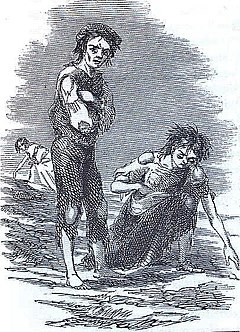
\includegraphics[width=1.36458in,height=\textheight]{./imgs/intro_famine.JPG}}A
famous example of pandemics is the Irish potato famine of 1845--1847
caused by the late blight pathogen (\emph{Phytophthora infestans}), the
cause of a disease that changed the history of Europe and the United
States, and that is also known for its role in developing the science of
plant pathology. During the 1840s, the disease devastated potato crops,
a staple food of the Irish at the time. The disease was triggered by the
introduction of a new virulent pathogen population that found the right
environmental conditions (cool and wet weather) for infection and
development in a highly dense population of susceptible hosts.
\end{tcolorbox}

Botanical epidemiology, or the study of plant disease epidemics, is a
relatively young discipline formally recognized in 1963. Two important
facts marked that year. J.E. Vanderplank published his famous book
``Plant Disease Epidemic and Control'' (Vanderplank 1963) and the first
International Epidemiology Workshop was held in Pau, France. Vanderplank
is fully acknowledged as the founding father of plant disease
epidemiology (Zadoks and Schein 1988; Thresh 1998)

\part{Epidemic data}

\hypertarget{disease-variables}{%
\chapter{Disease variables}\label{disease-variables}}

\begin{tcolorbox}[enhanced jigsaw, rightrule=.15mm, left=2mm, breakable, colframe=quarto-callout-note-color-frame, toprule=.15mm, leftrule=.75mm, bottomrule=.15mm, colback=white, arc=.35mm, opacityback=0]
\begin{minipage}[t]{5.5mm}
\textcolor{quarto-callout-note-color}{\faInfo}
\end{minipage}%
\begin{minipage}[t]{\textwidth - 5.5mm}
This is a work in progress that is currently undergoing heavy technical
editing and copy-editing\end{minipage}%
\end{tcolorbox}

\hypertarget{phytopathometry}{%
\section{Phytopathometry}\label{phytopathometry}}

Studies on the progress of epidemics in time or their spread in space
cannot be conducted without data collected in the field - or in same
cases simulated. The study of plant disease quantification is known as
Phytopathometry, a branch of plant pathology tasked with the science of
disease measurement, but which has strong roots in epidemiology (Bock et
al. 2021). Historically, disease quantification has been performed
visually, but advances in both imaging and remote sensing technologies
have directly impacted the field during the last several decades.
Therefore, the quantity of disease can be obtained via estimation
(visually by human eye) or measurement (sensor or digital technologies:
RGB, MSI, HSI). This means that several variables can be used to express
disease occurrence and quantity.

\begin{figure}

{\centering 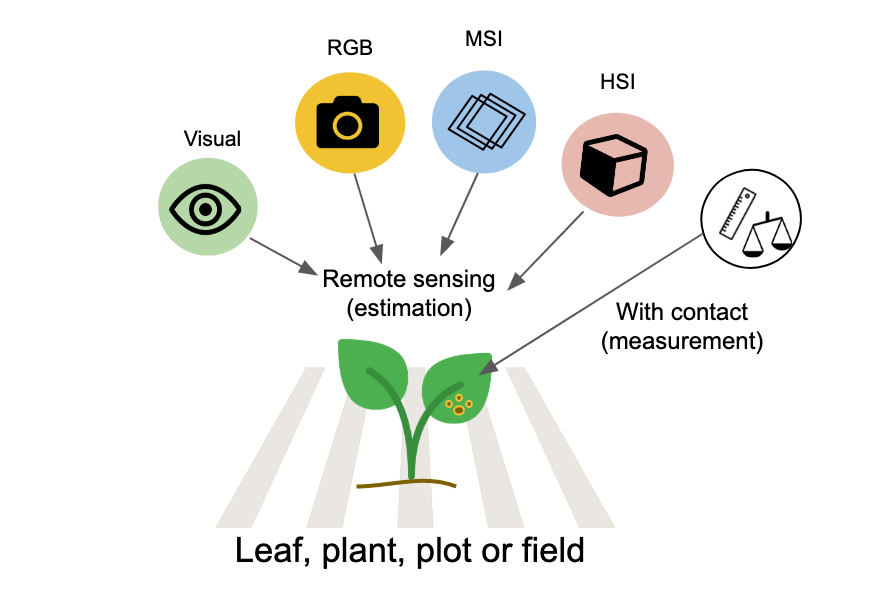
\includegraphics[width=5.10417in,height=\textheight]{./imgs/disease_measure.png}

}

\caption{Different approaches used to obtain estimates or measures of
plant disease}

\end{figure}

While measuring disease is a a more objective task, visual assessment is
largely subjective and, as such, known to vary among human raters. This
occurs because raters vary in their inherent abilities, training, or are
more or less affected by the chosen method (e.g.~scales). Disease is
estimated or measured on a specimen in a population, or on a sample of
specimens drawn from a population. The specimen can be a plant organ, an
individual plant, a group of plants, a field or a farm, and these also
dictate how terms are defined to refer to disease quantity.

Finally, when developing new or improving existing disease assessment
methods, it is important to assess how close the estimations or
measurements are from reference (gold standard) values. There are
several methods that can be used to assess reliability, precision and
accuracy of estimates or measures. The choice depends on the objective
of the work but largely on the type or nature of the data, as it will be
discussed further.

\hypertarget{terminology}{%
\section{Terminology}\label{terminology}}

A general term used to refer to the quantity of disease expressed by any
means is \textbf{disease intensity}. This term has little or no
practical value as it only suggest that the disease is more or less
``intense''. We need more specific terms to refer to disease quantity. A
primary task in disease assessment is to classify each specimen, usually
in a sample or in the population, as diseased or not diseased. This
binary (yes/no) assessment may be sufficient to express disease
intensity if the goal is to assess, for example, the number or
proportion of diseased specimens in a sample or a population of
specimens.

The above leads to two terms: disease \textbf{incidence} and
\textbf{prevalence}. While incidence is commonly used to refer to the
proportion or number (count) of plants (or their organs) as the
observational units at the field scale or below, prevalence is used when
referring to the proportion or number of fields or farms with diseased
plants in a large production area or region (Nutter et al. 2006). Hence,
prevalence is equivalent to incidence, only differing in the spatial
scale of the sampling unit.

\begin{figure}

{\centering 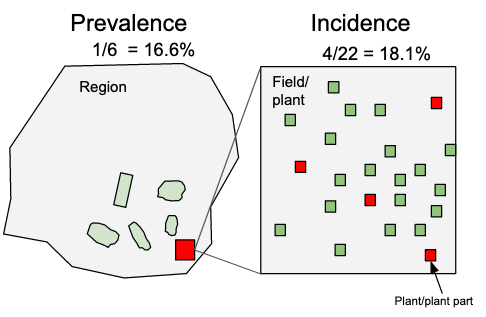
\includegraphics[width=5in,height=\textheight]{./imgs/prevalence_incidence.png}

}

\caption{Schematic representation of prevalence and incidence of plant
diseases}

\end{figure}

In many cases we need to ascertain the \emph{degree to which a specimen
is diseased}, which is a definition of disease \textbf{severity}.
Elsewhere, severity is defined restrictively as the proportion of the
unit that is symptomatic (Nutter et al. 2006). However, a broader view
of severity encompasses other metrics including lesion counts and scores
based on ordinal scales. These latter scales can be further divided into
classes defined based on either the percentage scale or descriptions of
symptoms (Bock et al. 2021). In some cases disease is expressed in terms
of (average) lesion size or area, which can be considered a measure of
severity. It is commonly used to determine host resistance, pathogen
aggressiveness or environmental influence.

\begin{figure}

{\centering 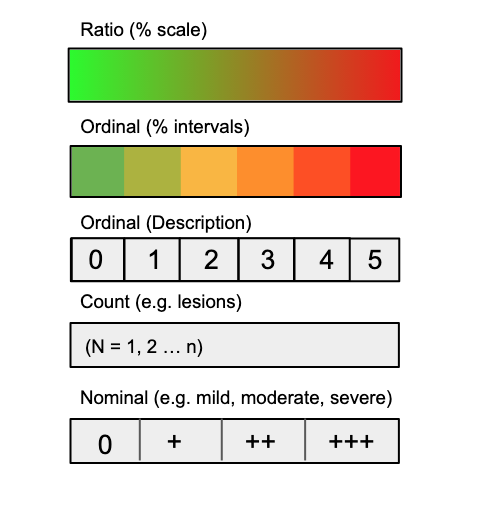
\includegraphics[width=4.58333in,height=\textheight]{./imgs/severity.png}

}

\caption{Different scales and variable types used to represent severity
of plant diseases}

\end{figure}

\hypertarget{data-types-and-distributions}{%
\chapter{Data types and
distributions}\label{data-types-and-distributions}}

\begin{tcolorbox}[enhanced jigsaw, rightrule=.15mm, left=2mm, breakable, colframe=quarto-callout-note-color-frame, toprule=.15mm, leftrule=.75mm, bottomrule=.15mm, colback=white, arc=.35mm, opacityback=0]
\begin{minipage}[t]{5.5mm}
\textcolor{quarto-callout-note-color}{\faInfo}
\end{minipage}%
\begin{minipage}[t]{\textwidth - 5.5mm}
This is a work in progress that is currently undergoing heavy technical
editing and copy-editing\end{minipage}%
\end{tcolorbox}

The data used to express disease as incidence or any kind of severity
measures vary in their nature as they can be discrete or continuous.

\textbf{Discrete} variables are countable (involve integers) at a finite
amount of time. That is, only a limited number of values (nominal or
ordinal) is possible and these cannot be subdivided into parts. For
example, a plant or plant part can be either disease or not diseased
(nominal data). One can't count 1.5 diseased plants. Also, a plant
classified as diseased may exhibit a certain number of lesions (count
data) or be classified into a specific class of severity (ordinal data,
common in ordinal scales, e.g., 1-9). Disease data in the form of counts
usually relate to the number of infections per sampling units. Most
commonly, counts refer to the pathogen population that is assessed, such
as number of airborne or soilborne propagules.

A \textbf{continuous} variable, different from discrete, can be measured
on a scale and can have any numeric value between two numbers. For
example, the size of a lesion on a plant can be measured at a very
precise scale (cm or mm). An estimate of severity in percent scale (\%
diseased area) can take any value between non zero and 100\%. Although
discrete at the individual level, incidence at the sample level can be
treated as continuous, as it can take any value in proportion or
percentage.

The disease variables can also be described by a statistical
distribution, which are models that give the probability that a
particular value (or a range of values) will be drawn from a specific
distribution. Knowledge about statistical or mathematical distributions
constitute an important step to improve our understanding of
data-collection methods, designs of experiments and data analysis such
as data summarization or hypothesis testing.

\hypertarget{statistical-distributions}{%
\section{Statistical distributions}\label{statistical-distributions}}

\hypertarget{binomial-distribution}{%
\subsection{Binomial distribution}\label{binomial-distribution}}

For incidence (and prevalence), the data is binary at the individual
level, as there are only two possible outcomes in a \emph{trial}: the
plant or plant part is disease or not diseased. The statistical
distribution that best describe the incidence data at the individual
level is the \emph{binomial distribution}.

Let's simulate the binomial outcomes for a range of probabilities in a
sample of 100 units, using the \texttt{rbinom()} function in R. For a
single trial (e.g., status of plants in a single plant row), the
\texttt{size} argument is set to 1.

\begin{Shaded}
\begin{Highlighting}[]
\FunctionTok{library}\NormalTok{(tidyverse)}
\FunctionTok{theme\_set}\NormalTok{(}\FunctionTok{theme\_bw}\NormalTok{(}\AttributeTok{base\_size =} \DecValTok{14}\NormalTok{)) }\CommentTok{\# set global theme}

\FunctionTok{set.seed}\NormalTok{(}\DecValTok{123}\NormalTok{) }\CommentTok{\# for reproducibility}
\NormalTok{P}\FloatTok{.1} \OtherTok{\textless{}{-}} \FunctionTok{rbinom}\NormalTok{(}\DecValTok{100}\NormalTok{, }\AttributeTok{size =} \DecValTok{1}\NormalTok{, }\AttributeTok{prob =} \FloatTok{0.1}\NormalTok{)}
\NormalTok{P}\FloatTok{.3} \OtherTok{\textless{}{-}} \FunctionTok{rbinom}\NormalTok{(}\DecValTok{100}\NormalTok{, }\AttributeTok{size =} \DecValTok{1}\NormalTok{, }\AttributeTok{prob =} \FloatTok{0.3}\NormalTok{)}
\NormalTok{P}\FloatTok{.7} \OtherTok{\textless{}{-}} \FunctionTok{rbinom}\NormalTok{(}\DecValTok{100}\NormalTok{, }\AttributeTok{size =} \DecValTok{1}\NormalTok{, }\AttributeTok{prob =} \FloatTok{0.7}\NormalTok{)}
\NormalTok{P}\FloatTok{.9} \OtherTok{\textless{}{-}} \FunctionTok{rbinom}\NormalTok{(}\DecValTok{100}\NormalTok{, }\AttributeTok{size =} \DecValTok{1}\NormalTok{, }\AttributeTok{prob =} \FloatTok{0.9}\NormalTok{)}
\NormalTok{binomial\_data }\OtherTok{\textless{}{-}} \FunctionTok{data.frame}\NormalTok{(P}\FloatTok{.1}\NormalTok{, P}\FloatTok{.3}\NormalTok{, P}\FloatTok{.7}\NormalTok{, P}\FloatTok{.9}\NormalTok{)}
\end{Highlighting}
\end{Shaded}

We can then visualize the plots.

\begin{Shaded}
\begin{Highlighting}[]
\NormalTok{binomial\_data }\SpecialCharTok{|\textgreater{}}
  \FunctionTok{pivot\_longer}\NormalTok{(}\DecValTok{1}\SpecialCharTok{:}\DecValTok{4}\NormalTok{, }\AttributeTok{names\_to =} \StringTok{"P"}\NormalTok{,}
               \AttributeTok{values\_to =} \StringTok{"value"}\NormalTok{) }\SpecialCharTok{|\textgreater{}}
  \FunctionTok{ggplot}\NormalTok{(}\FunctionTok{aes}\NormalTok{(value)) }\SpecialCharTok{+}
  \FunctionTok{geom\_histogram}\NormalTok{(}\AttributeTok{fill =} \StringTok{"darkorange"}\NormalTok{,}
                 \AttributeTok{bins =} \DecValTok{10}\NormalTok{) }\SpecialCharTok{+}
  \FunctionTok{facet\_wrap}\NormalTok{( }\SpecialCharTok{\textasciitilde{}}\NormalTok{ P) }
\end{Highlighting}
\end{Shaded}

\begin{figure}[H]

{\centering 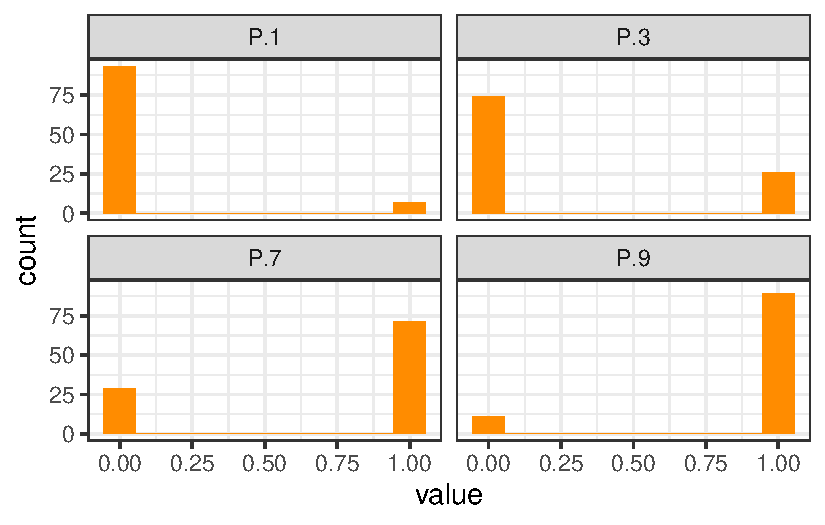
\includegraphics{./data-type-distributions_files/figure-pdf/fig-binomial-1.pdf}

}

\caption{\label{fig-binomial}Binomial distribution to describe binary
data}

\end{figure}

\hypertarget{beta-distribution}{%
\subsection{Beta distribution}\label{beta-distribution}}

Disease incidence (or prevalence) at the sample or population level can
be expressed as proportion of diseased individuals. The same applies to
disease severity when expressed as proportion of the organ area affected
(a ratio variable). For such cases, the beta distribution, which is
bounded between 0 and 1, provides a good description. Let's simulate
some data using the \texttt{rbeta()} function.

\begin{Shaded}
\begin{Highlighting}[]
\NormalTok{beta1}\FloatTok{.5} \OtherTok{\textless{}{-}} \FunctionTok{rbeta}\NormalTok{(}\AttributeTok{n =} \DecValTok{1000}\NormalTok{, }\AttributeTok{shape1 =} \DecValTok{1}\NormalTok{, }\AttributeTok{shape2 =} \DecValTok{5}\NormalTok{)}
\NormalTok{beta5}\FloatTok{.5} \OtherTok{\textless{}{-}} \FunctionTok{rbeta}\NormalTok{(}\AttributeTok{n =} \DecValTok{1000}\NormalTok{, }\AttributeTok{shape1 =} \DecValTok{5}\NormalTok{, }\AttributeTok{shape2 =} \DecValTok{5}\NormalTok{)}
\NormalTok{beta\_data }\OtherTok{\textless{}{-}} \FunctionTok{data.frame}\NormalTok{(beta1}\FloatTok{.5}\NormalTok{, beta5}\FloatTok{.5}\NormalTok{)}
\end{Highlighting}
\end{Shaded}

Notice that there are two shape parameters in the beta distribution:
\texttt{shape1} and \texttt{shape2} to be defined. This makes the
distribution very flexible and with different potential shapes as we can
see below.

\begin{Shaded}
\begin{Highlighting}[]
\FunctionTok{library}\NormalTok{(tidyverse)}
\FunctionTok{theme\_set}\NormalTok{(}\FunctionTok{theme\_bw}\NormalTok{(}\AttributeTok{base\_size =} \DecValTok{14}\NormalTok{)) }\CommentTok{\# set global theme}

\NormalTok{beta\_data }\SpecialCharTok{|\textgreater{}}
  \FunctionTok{pivot\_longer}\NormalTok{(}\DecValTok{1}\SpecialCharTok{:}\DecValTok{2}\NormalTok{, }\AttributeTok{names\_to =} \StringTok{"P"}\NormalTok{,}
               \AttributeTok{values\_to =} \StringTok{"value"}\NormalTok{) }\SpecialCharTok{|\textgreater{}}
  \FunctionTok{ggplot}\NormalTok{(}\FunctionTok{aes}\NormalTok{(value)) }\SpecialCharTok{+}
  \FunctionTok{geom\_histogram}\NormalTok{(}\AttributeTok{fill =} \StringTok{"darkorange"}\NormalTok{,}
                 \AttributeTok{color =} \StringTok{"white"}\NormalTok{,}
                 \AttributeTok{bins =} \DecValTok{15}\NormalTok{) }\SpecialCharTok{+}
  \FunctionTok{scale\_x\_continuous}\NormalTok{(}\AttributeTok{limits =} \FunctionTok{c}\NormalTok{(}\DecValTok{0}\NormalTok{, }\DecValTok{1}\NormalTok{)) }\SpecialCharTok{+}
  \FunctionTok{facet\_wrap}\NormalTok{( }\SpecialCharTok{\textasciitilde{}}\NormalTok{ P) }
\end{Highlighting}
\end{Shaded}

\begin{figure}[H]

{\centering 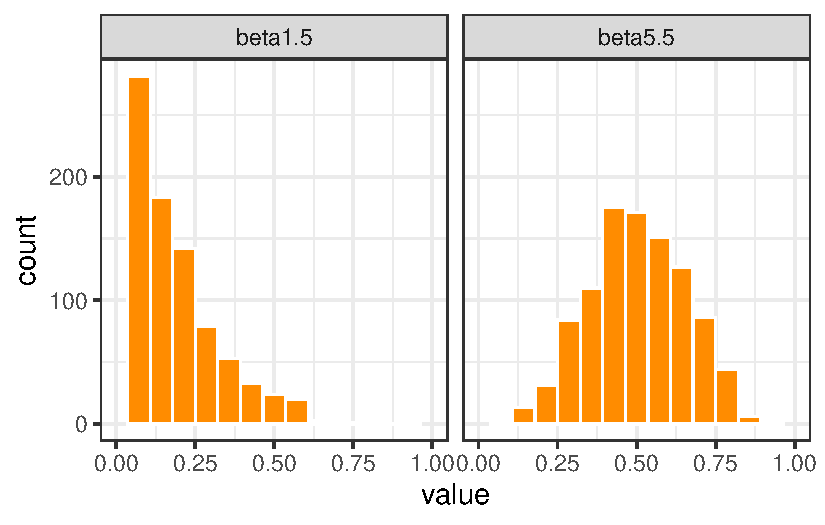
\includegraphics{./data-type-distributions_files/figure-pdf/fig-beta-1.pdf}

}

\caption{\label{fig-beta}Binomial distribution to describe proportion
data}

\end{figure}

\hypertarget{poisson-distribution}{%
\subsection{Poisson distribution}\label{poisson-distribution}}

The number of diseased plants, plant parts or individual symptoms
(lesions) are discrete variables (integers) which cannot take negative
values. These can be described by a Poisson distribution, a discrete
distribution that counts the number of events in a Poisson process. In
R, we can used the \texttt{rpois()} function to obtain 100 random
observations following a Poisson distribution. For such, we need to
inform the number of observation (n = 100) and \texttt{lambda}, the
vector of means.

\begin{Shaded}
\begin{Highlighting}[]
\NormalTok{poisson5 }\OtherTok{\textless{}{-}} \FunctionTok{rpois}\NormalTok{(}\DecValTok{100}\NormalTok{, }\AttributeTok{lambda =} \DecValTok{10}\NormalTok{)}
\NormalTok{poisson35 }\OtherTok{\textless{}{-}} \FunctionTok{rpois}\NormalTok{(}\DecValTok{100}\NormalTok{, }\AttributeTok{lambda =} \DecValTok{35}\NormalTok{)}
\NormalTok{poisson\_data }\OtherTok{\textless{}{-}} \FunctionTok{data.frame}\NormalTok{(poisson5, poisson35)}
\end{Highlighting}
\end{Shaded}

\begin{Shaded}
\begin{Highlighting}[]
\NormalTok{poisson\_data }\SpecialCharTok{|\textgreater{}}
  \FunctionTok{pivot\_longer}\NormalTok{(}\DecValTok{1}\SpecialCharTok{:}\DecValTok{2}\NormalTok{, }\AttributeTok{names\_to =} \StringTok{"P"}\NormalTok{,}
               \AttributeTok{values\_to =} \StringTok{"value"}\NormalTok{) }\SpecialCharTok{|\textgreater{}}
  \FunctionTok{ggplot}\NormalTok{(}\FunctionTok{aes}\NormalTok{(value)) }\SpecialCharTok{+}
  \FunctionTok{geom\_histogram}\NormalTok{(}\AttributeTok{fill =} \StringTok{"darkorange"}\NormalTok{,}
                 \AttributeTok{color =} \StringTok{"white"}\NormalTok{,}
                 \AttributeTok{bins =} \DecValTok{15}\NormalTok{) }\SpecialCharTok{+}
  \FunctionTok{facet\_wrap}\NormalTok{( }\SpecialCharTok{\textasciitilde{}}\NormalTok{ P) }
\end{Highlighting}
\end{Shaded}

\begin{figure}[H]

{\centering 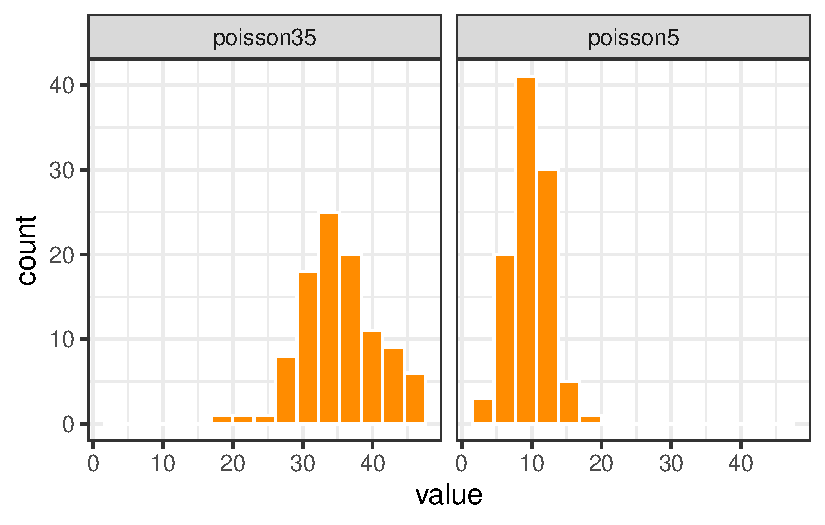
\includegraphics{./data-type-distributions_files/figure-pdf/fig-poisson-1.pdf}

}

\caption{\label{fig-poisson}Binomial distribution to describe count
data}

\end{figure}

\hypertarget{gamma-distribution}{%
\subsection{Gamma distribution}\label{gamma-distribution}}

When working with a continuous variables, such as lesion size, these
random variables are usually described by the normal distribution.
However, the problem is that the normal (Gaussian) distribution includes
negative values, an unrealistic situation. Therefore, we can use the
gamma distribution, which cannot take negative values, to simulate
continuous plant disease data. We can use the \texttt{rgamma()} function
that requires the number of samples (n = 100 in our case) and the
\texttt{shape}, or the mean value.

\begin{Shaded}
\begin{Highlighting}[]
\NormalTok{gamma10 }\OtherTok{\textless{}{-}} \FunctionTok{rgamma}\NormalTok{(}\AttributeTok{n =} \DecValTok{100}\NormalTok{, }\AttributeTok{shape =} \DecValTok{10}\NormalTok{, }\AttributeTok{scale =} \DecValTok{1}\NormalTok{)}
\NormalTok{gamma35 }\OtherTok{\textless{}{-}} \FunctionTok{rgamma}\NormalTok{(}\AttributeTok{n =} \DecValTok{100}\NormalTok{, }\AttributeTok{shape =} \DecValTok{35}\NormalTok{, }\AttributeTok{scale =} \DecValTok{1}\NormalTok{)}
\NormalTok{gamma\_data }\OtherTok{\textless{}{-}} \FunctionTok{data.frame}\NormalTok{(gamma10, gamma35)}
\end{Highlighting}
\end{Shaded}

\begin{Shaded}
\begin{Highlighting}[]
\NormalTok{gamma\_data }\SpecialCharTok{|\textgreater{}}
  \FunctionTok{pivot\_longer}\NormalTok{(}\DecValTok{1}\SpecialCharTok{:}\DecValTok{2}\NormalTok{, }\AttributeTok{names\_to =} \StringTok{"P"}\NormalTok{,}
               \AttributeTok{values\_to =} \StringTok{"value"}\NormalTok{) }\SpecialCharTok{|\textgreater{}}
  \FunctionTok{ggplot}\NormalTok{(}\FunctionTok{aes}\NormalTok{(value)) }\SpecialCharTok{+}
  \FunctionTok{geom\_histogram}\NormalTok{(}\AttributeTok{fill =} \StringTok{"darkorange"}\NormalTok{,}
                 \AttributeTok{color =} \StringTok{"white"}\NormalTok{,}
                 \AttributeTok{bins =} \DecValTok{15}\NormalTok{) }\SpecialCharTok{+}
  \FunctionTok{ylim}\NormalTok{(}\DecValTok{0}\NormalTok{, }\FunctionTok{max}\NormalTok{(gamma\_data}\SpecialCharTok{$}\NormalTok{gamma35)) }\SpecialCharTok{+}
  \FunctionTok{facet\_wrap}\NormalTok{( }\SpecialCharTok{\textasciitilde{}}\NormalTok{ P) }
\end{Highlighting}
\end{Shaded}

\begin{figure}[H]

{\centering 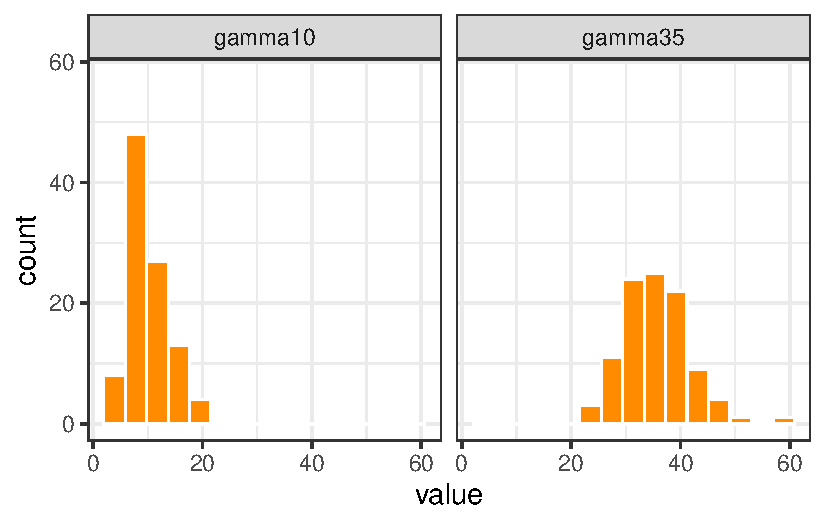
\includegraphics{./data-type-distributions_files/figure-pdf/fig-gamma-1.pdf}

}

\caption{\label{fig-gamma}Gamma distribution to describe continuous
data}

\end{figure}

\hypertarget{reliability-and-accuracy}{%
\chapter{Reliability and accuracy}\label{reliability-and-accuracy}}

\begin{tcolorbox}[enhanced jigsaw, rightrule=.15mm, left=2mm, breakable, colframe=quarto-callout-note-color-frame, toprule=.15mm, leftrule=.75mm, bottomrule=.15mm, colback=white, arc=.35mm, opacityback=0]
\begin{minipage}[t]{5.5mm}
\textcolor{quarto-callout-note-color}{\faInfo}
\end{minipage}%
\begin{minipage}[t]{\textwidth - 5.5mm}
This is a work in progress that is currently undergoing heavy technical
editing and copy-editing\end{minipage}%
\end{tcolorbox}

Disease severity, mainly when expressed in percent area diseased
assessed visually, is acknowledged as a more difficult and less time-
and cost-effective plant disease variable to obtain. However, errors may
occur even when assessing a more objective measure such as incidence.
This is the case when an incorrect assignment or confusion of symptoms
occur. In either case, the quality of the assessment of any disease
variable is very important and should be gauged in the studies. Several
terms can be used when evaluating the quality of disease assessments,
including reliability, precision, accuracy or agreement.

\textbf{Reliability}: The extent to which the same estimates or
measurements of diseased specimens obtained under different conditions
yield similar results. There are two types. The \emph{inter-rater
reliability} (or reproducibility) is a measure of consistency of disease
assessment across the same specimens between raters or devices. The
\emph{intra-rater} reliability (or repeatability) measures consistency
by the same rater or instrument on the same specimens (e.g.~two
assessments in time by the same rater).

\begin{figure}

{\centering 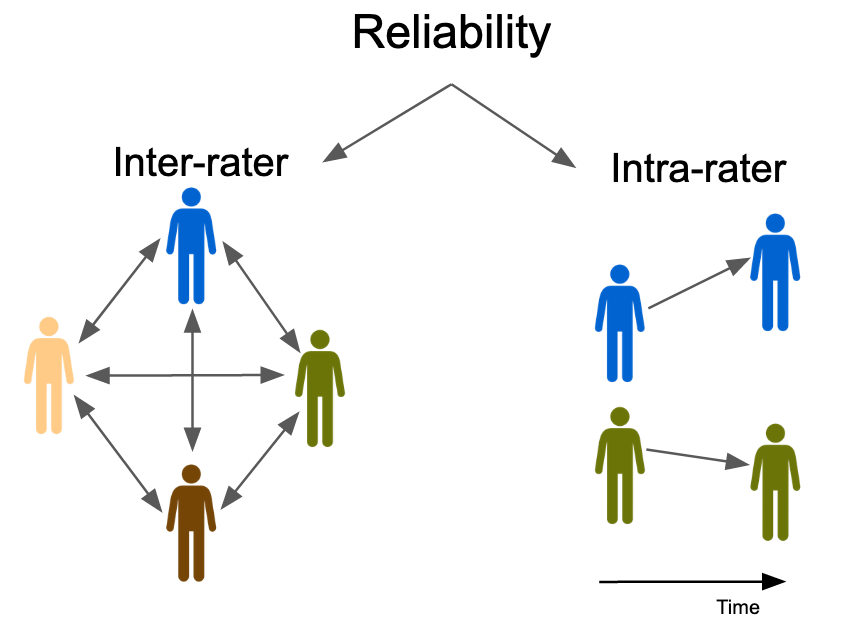
\includegraphics[width=5.26042in,height=\textheight]{./imgs/reliability.png}

}

\caption{\label{fig-reliability.png}Two types of reliability of
estimates or measures of plant disease intensity}

\end{figure}

\textbf{Precision:} A statistical term to express the measure of
variability of the estimates or measurements of disease on the same
specimens obtained by different raters (or instruments). However,
reliable or precise estimates (or measurements) are not necessarily
close to an actual value, but precision is a component of accuracy or
agreement.

\textbf{Accuracy or agreement}: These two terms can be treated as
synonymous in plant pathological research. They refer to the closeness
(or concordance) of an estimate or measurement to the actual severity
value for a specimen on the same scale. Actual values may be obtained
using various methods, against which estimates or measurements using an
experimental assessment method are compared.

An analogy commonly used to explain accuracy and precision is the archer
shooting arrows at a target and trying to hit the bull's eye (center of
the target) with each of five arrows. The figure below is used to
demonstrate four situations from the combination of two levels (high and
low) for precision and accuracy. The figure was produced using the
\texttt{ggplot} function of \emph{ggplot2} package.

\begin{Shaded}
\begin{Highlighting}[]
\FunctionTok{library}\NormalTok{(ggplot2)}
\NormalTok{target }\OtherTok{\textless{}{-}} 
  \FunctionTok{ggplot}\NormalTok{(}\FunctionTok{data.frame}\NormalTok{(}\FunctionTok{c}\NormalTok{(}\DecValTok{1}\SpecialCharTok{:}\DecValTok{10}\NormalTok{),}\FunctionTok{c}\NormalTok{(}\DecValTok{1}\SpecialCharTok{:}\DecValTok{10}\NormalTok{)))}\SpecialCharTok{+}
  \FunctionTok{geom\_point}\NormalTok{(}\FunctionTok{aes}\NormalTok{(}\AttributeTok{x =} \DecValTok{5}\NormalTok{, }\AttributeTok{y =} \DecValTok{5}\NormalTok{), }\AttributeTok{size =} \FloatTok{71.5}\NormalTok{, }\AttributeTok{color =} \StringTok{"black"}\NormalTok{)}\SpecialCharTok{+}
  \FunctionTok{geom\_point}\NormalTok{(}\FunctionTok{aes}\NormalTok{(}\AttributeTok{x =} \DecValTok{5}\NormalTok{, }\AttributeTok{y =} \DecValTok{5}\NormalTok{), }\AttributeTok{size =} \DecValTok{70}\NormalTok{, }\AttributeTok{color =} \StringTok{"orange"}\NormalTok{)}\SpecialCharTok{+}
  \FunctionTok{geom\_point}\NormalTok{(}\FunctionTok{aes}\NormalTok{(}\AttributeTok{x =} \DecValTok{5}\NormalTok{, }\AttributeTok{y =} \DecValTok{5}\NormalTok{), }\AttributeTok{size =} \DecValTok{60}\NormalTok{, }\AttributeTok{color =} \StringTok{"white"}\NormalTok{)}\SpecialCharTok{+}
  \FunctionTok{geom\_point}\NormalTok{(}\FunctionTok{aes}\NormalTok{(}\AttributeTok{x =} \DecValTok{5}\NormalTok{, }\AttributeTok{y =} \DecValTok{5}\NormalTok{), }\AttributeTok{size =} \DecValTok{50}\NormalTok{, }\AttributeTok{color =} \StringTok{"orange"}\NormalTok{)}\SpecialCharTok{+}
  \FunctionTok{geom\_point}\NormalTok{(}\FunctionTok{aes}\NormalTok{(}\AttributeTok{x =} \DecValTok{5}\NormalTok{, }\AttributeTok{y =} \DecValTok{5}\NormalTok{), }\AttributeTok{size =} \DecValTok{40}\NormalTok{, }\AttributeTok{color =} \StringTok{"white"}\NormalTok{)}\SpecialCharTok{+}
  \FunctionTok{geom\_point}\NormalTok{(}\FunctionTok{aes}\NormalTok{(}\AttributeTok{x =} \DecValTok{5}\NormalTok{, }\AttributeTok{y =} \DecValTok{5}\NormalTok{), }\AttributeTok{size =} \DecValTok{30}\NormalTok{, }\AttributeTok{color =} \StringTok{"orange"}\NormalTok{)}\SpecialCharTok{+}
  \FunctionTok{geom\_point}\NormalTok{(}\FunctionTok{aes}\NormalTok{(}\AttributeTok{x =} \DecValTok{5}\NormalTok{, }\AttributeTok{y =} \DecValTok{5}\NormalTok{), }\AttributeTok{size =} \DecValTok{20}\NormalTok{, }\AttributeTok{color =} \StringTok{"white"}\NormalTok{)}\SpecialCharTok{+}
  \FunctionTok{geom\_point}\NormalTok{(}\FunctionTok{aes}\NormalTok{(}\AttributeTok{x =} \DecValTok{5}\NormalTok{, }\AttributeTok{y =} \DecValTok{5}\NormalTok{), }\AttributeTok{size =} \DecValTok{10}\NormalTok{, }\AttributeTok{color =} \StringTok{"orange"}\NormalTok{)}\SpecialCharTok{+}
  \FunctionTok{geom\_point}\NormalTok{(}\FunctionTok{aes}\NormalTok{(}\AttributeTok{x =} \DecValTok{5}\NormalTok{, }\AttributeTok{y =} \DecValTok{5}\NormalTok{), }\AttributeTok{size =} \DecValTok{4}\NormalTok{, }\AttributeTok{color =} \StringTok{"white"}\NormalTok{)}\SpecialCharTok{+}
  \FunctionTok{ylim}\NormalTok{(}\DecValTok{0}\NormalTok{,}\DecValTok{10}\NormalTok{)}\SpecialCharTok{+}
  \FunctionTok{xlim}\NormalTok{(}\DecValTok{0}\NormalTok{,}\DecValTok{10}\NormalTok{)}\SpecialCharTok{+}
  \FunctionTok{theme\_void}\NormalTok{()}

\NormalTok{hahp }\OtherTok{\textless{}{-}}\NormalTok{ target }\SpecialCharTok{+}
  \FunctionTok{labs}\NormalTok{(}\AttributeTok{subtitle =} \StringTok{"High Accuracy High Precision"}\NormalTok{)}\SpecialCharTok{+}
  \FunctionTok{theme}\NormalTok{(}\AttributeTok{plot.subtitle =} \FunctionTok{element\_text}\NormalTok{(}\AttributeTok{hjust =} \FloatTok{0.5}\NormalTok{))}\SpecialCharTok{+}
  \FunctionTok{geom\_point}\NormalTok{(}\FunctionTok{aes}\NormalTok{(}\AttributeTok{x =} \DecValTok{5}\NormalTok{, }\AttributeTok{y =} \DecValTok{5}\NormalTok{), }\AttributeTok{shape =} \DecValTok{4}\NormalTok{, }\AttributeTok{size =}\DecValTok{2}\NormalTok{, }\AttributeTok{color =} \StringTok{"blue"}\NormalTok{)}\SpecialCharTok{+}
  \FunctionTok{geom\_point}\NormalTok{(}\FunctionTok{aes}\NormalTok{(}\AttributeTok{x =} \DecValTok{5}\NormalTok{, }\AttributeTok{y =} \FloatTok{5.2}\NormalTok{), }\AttributeTok{shape =} \DecValTok{4}\NormalTok{, }\AttributeTok{size =}\DecValTok{2}\NormalTok{, }\AttributeTok{color =} \StringTok{"blue"}\NormalTok{)}\SpecialCharTok{+}
  \FunctionTok{geom\_point}\NormalTok{(}\FunctionTok{aes}\NormalTok{(}\AttributeTok{x =} \DecValTok{5}\NormalTok{, }\AttributeTok{y =} \FloatTok{4.8}\NormalTok{), }\AttributeTok{shape =} \DecValTok{4}\NormalTok{, }\AttributeTok{size =}\DecValTok{2}\NormalTok{, }\AttributeTok{color =} \StringTok{"blue"}\NormalTok{)}\SpecialCharTok{+}
  \FunctionTok{geom\_point}\NormalTok{(}\FunctionTok{aes}\NormalTok{(}\AttributeTok{x =} \FloatTok{4.8}\NormalTok{, }\AttributeTok{y =} \DecValTok{5}\NormalTok{), }\AttributeTok{shape =} \DecValTok{4}\NormalTok{, }\AttributeTok{size =}\DecValTok{2}\NormalTok{, }\AttributeTok{color =} \StringTok{"blue"}\NormalTok{)}\SpecialCharTok{+}
  \FunctionTok{geom\_point}\NormalTok{(}\FunctionTok{aes}\NormalTok{(}\AttributeTok{x =} \FloatTok{5.2}\NormalTok{, }\AttributeTok{y =} \DecValTok{5}\NormalTok{), }\AttributeTok{shape =} \DecValTok{4}\NormalTok{, }\AttributeTok{size =}\DecValTok{2}\NormalTok{, }\AttributeTok{color =} \StringTok{"blue"}\NormalTok{)}


\NormalTok{lahp }\OtherTok{\textless{}{-}}\NormalTok{ target }\SpecialCharTok{+}
  \FunctionTok{labs}\NormalTok{(}\AttributeTok{subtitle =} \StringTok{"Low Accuracy High Precision"}\NormalTok{)}\SpecialCharTok{+}
  \FunctionTok{theme}\NormalTok{(}\AttributeTok{plot.subtitle =} \FunctionTok{element\_text}\NormalTok{(}\AttributeTok{hjust =} \FloatTok{0.5}\NormalTok{))}\SpecialCharTok{+}
  \FunctionTok{geom\_point}\NormalTok{(}\FunctionTok{aes}\NormalTok{(}\AttributeTok{x =} \DecValTok{6}\NormalTok{, }\AttributeTok{y =} \DecValTok{6}\NormalTok{), }\AttributeTok{shape =} \DecValTok{4}\NormalTok{, }\AttributeTok{size =}\DecValTok{2}\NormalTok{, }\AttributeTok{color =} \StringTok{"blue"}\NormalTok{)}\SpecialCharTok{+}
  \FunctionTok{geom\_point}\NormalTok{(}\FunctionTok{aes}\NormalTok{(}\AttributeTok{x =} \DecValTok{6}\NormalTok{, }\AttributeTok{y =} \FloatTok{6.2}\NormalTok{), }\AttributeTok{shape =} \DecValTok{4}\NormalTok{, }\AttributeTok{size =}\DecValTok{2}\NormalTok{, }\AttributeTok{color =} \StringTok{"blue"}\NormalTok{)}\SpecialCharTok{+}
  \FunctionTok{geom\_point}\NormalTok{(}\FunctionTok{aes}\NormalTok{(}\AttributeTok{x =} \DecValTok{6}\NormalTok{, }\AttributeTok{y =} \FloatTok{5.8}\NormalTok{), }\AttributeTok{shape =} \DecValTok{4}\NormalTok{, }\AttributeTok{size =}\DecValTok{2}\NormalTok{, }\AttributeTok{color =} \StringTok{"blue"}\NormalTok{)}\SpecialCharTok{+}
  \FunctionTok{geom\_point}\NormalTok{(}\FunctionTok{aes}\NormalTok{(}\AttributeTok{x =} \FloatTok{5.8}\NormalTok{, }\AttributeTok{y =} \DecValTok{6}\NormalTok{), }\AttributeTok{shape =} \DecValTok{4}\NormalTok{, }\AttributeTok{size =}\DecValTok{2}\NormalTok{, }\AttributeTok{color =} \StringTok{"blue"}\NormalTok{)}\SpecialCharTok{+}
  \FunctionTok{geom\_point}\NormalTok{(}\FunctionTok{aes}\NormalTok{(}\AttributeTok{x =} \FloatTok{6.2}\NormalTok{, }\AttributeTok{y =} \DecValTok{6}\NormalTok{), }\AttributeTok{shape =} \DecValTok{4}\NormalTok{, }\AttributeTok{size =}\DecValTok{2}\NormalTok{, }\AttributeTok{color =} \StringTok{"blue"}\NormalTok{)}


\NormalTok{halp }\OtherTok{\textless{}{-}}\NormalTok{ target }\SpecialCharTok{+}
  \FunctionTok{labs}\NormalTok{(}\AttributeTok{subtitle =} \StringTok{"High Accuracy Low Precision"}\NormalTok{)}\SpecialCharTok{+}
  \FunctionTok{theme}\NormalTok{(}\AttributeTok{plot.subtitle =} \FunctionTok{element\_text}\NormalTok{(}\AttributeTok{hjust =} \FloatTok{0.5}\NormalTok{))}\SpecialCharTok{+}
  \FunctionTok{geom\_point}\NormalTok{(}\FunctionTok{aes}\NormalTok{(}\AttributeTok{x =} \DecValTok{5}\NormalTok{, }\AttributeTok{y =} \DecValTok{5}\NormalTok{), }\AttributeTok{shape =} \DecValTok{4}\NormalTok{, }\AttributeTok{size =}\DecValTok{2}\NormalTok{, }\AttributeTok{color =} \StringTok{"blue"}\NormalTok{)}\SpecialCharTok{+}
  \FunctionTok{geom\_point}\NormalTok{(}\FunctionTok{aes}\NormalTok{(}\AttributeTok{x =} \DecValTok{5}\NormalTok{, }\AttributeTok{y =} \FloatTok{5.8}\NormalTok{), }\AttributeTok{shape =} \DecValTok{4}\NormalTok{, }\AttributeTok{size =}\DecValTok{2}\NormalTok{, }\AttributeTok{color =} \StringTok{"blue"}\NormalTok{)}\SpecialCharTok{+}
  \FunctionTok{geom\_point}\NormalTok{(}\FunctionTok{aes}\NormalTok{(}\AttributeTok{x =} \FloatTok{5.8}\NormalTok{, }\AttributeTok{y =} \FloatTok{4.4}\NormalTok{), }\AttributeTok{shape =} \DecValTok{4}\NormalTok{, }\AttributeTok{size =}\DecValTok{2}\NormalTok{, }\AttributeTok{color =} \StringTok{"blue"}\NormalTok{)}\SpecialCharTok{+}
  \FunctionTok{geom\_point}\NormalTok{(}\FunctionTok{aes}\NormalTok{(}\AttributeTok{x =} \FloatTok{4.4}\NormalTok{, }\AttributeTok{y =} \DecValTok{5}\NormalTok{), }\AttributeTok{shape =} \DecValTok{4}\NormalTok{, }\AttributeTok{size =}\DecValTok{2}\NormalTok{, }\AttributeTok{color =} \StringTok{"blue"}\NormalTok{)}\SpecialCharTok{+}
  \FunctionTok{geom\_point}\NormalTok{(}\FunctionTok{aes}\NormalTok{(}\AttributeTok{x =} \FloatTok{5.6}\NormalTok{, }\AttributeTok{y =} \FloatTok{5.6}\NormalTok{), }\AttributeTok{shape =} \DecValTok{4}\NormalTok{, }\AttributeTok{size =}\DecValTok{2}\NormalTok{, }\AttributeTok{color =} \StringTok{"blue"}\NormalTok{)}

\NormalTok{lalp }\OtherTok{\textless{}{-}}\NormalTok{ target }\SpecialCharTok{+}
  \FunctionTok{labs}\NormalTok{(}\AttributeTok{subtitle =} \StringTok{"Low Accuracy Low Precision"}\NormalTok{)}\SpecialCharTok{+}
  \FunctionTok{theme}\NormalTok{(}\AttributeTok{plot.subtitle =} \FunctionTok{element\_text}\NormalTok{(}\AttributeTok{hjust =} \FloatTok{0.5}\NormalTok{))}\SpecialCharTok{+}
  \FunctionTok{geom\_point}\NormalTok{(}\FunctionTok{aes}\NormalTok{(}\AttributeTok{x =} \FloatTok{5.5}\NormalTok{, }\AttributeTok{y =} \FloatTok{5.5}\NormalTok{), }\AttributeTok{shape =} \DecValTok{4}\NormalTok{, }\AttributeTok{size =}\DecValTok{2}\NormalTok{, }\AttributeTok{color =} \StringTok{"blue"}\NormalTok{)}\SpecialCharTok{+}
  \FunctionTok{geom\_point}\NormalTok{(}\FunctionTok{aes}\NormalTok{(}\AttributeTok{x =} \FloatTok{4.5}\NormalTok{, }\AttributeTok{y =} \FloatTok{5.4}\NormalTok{), }\AttributeTok{shape =} \DecValTok{4}\NormalTok{, }\AttributeTok{size =}\DecValTok{2}\NormalTok{, }\AttributeTok{color =} \StringTok{"blue"}\NormalTok{)}\SpecialCharTok{+}
  \FunctionTok{geom\_point}\NormalTok{(}\FunctionTok{aes}\NormalTok{(}\AttributeTok{x =} \FloatTok{5.2}\NormalTok{, }\AttributeTok{y =} \FloatTok{6.8}\NormalTok{), }\AttributeTok{shape =} \DecValTok{4}\NormalTok{, }\AttributeTok{size =}\DecValTok{2}\NormalTok{, }\AttributeTok{color =} \StringTok{"blue"}\NormalTok{)}\SpecialCharTok{+}
  \FunctionTok{geom\_point}\NormalTok{(}\FunctionTok{aes}\NormalTok{(}\AttributeTok{x =} \FloatTok{4.8}\NormalTok{, }\AttributeTok{y =} \FloatTok{3.8}\NormalTok{), }\AttributeTok{shape =} \DecValTok{4}\NormalTok{, }\AttributeTok{size =}\DecValTok{2}\NormalTok{, }\AttributeTok{color =} \StringTok{"blue"}\NormalTok{)}\SpecialCharTok{+}
  \FunctionTok{geom\_point}\NormalTok{(}\FunctionTok{aes}\NormalTok{(}\AttributeTok{x =} \FloatTok{5.2}\NormalTok{, }\AttributeTok{y =} \DecValTok{3}\NormalTok{), }\AttributeTok{shape =} \DecValTok{4}\NormalTok{, }\AttributeTok{size =}\DecValTok{2}\NormalTok{, }\AttributeTok{color =} \StringTok{"blue"}\NormalTok{)}


\FunctionTok{library}\NormalTok{(patchwork)}
\NormalTok{(hahp }\SpecialCharTok{|}\NormalTok{ lahp) }\SpecialCharTok{/}
\NormalTok{(halp }\SpecialCharTok{|}\NormalTok{ lalp)}
\end{Highlighting}
\end{Shaded}

\begin{figure}[H]

{\centering 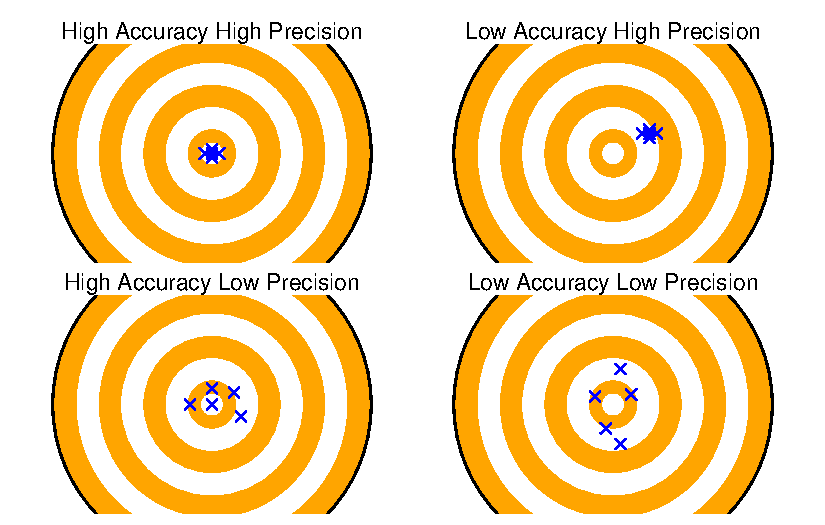
\includegraphics{./data-accuracy_files/figure-pdf/fig-target-1.pdf}

}

\caption{\label{fig-target}The accuracy and precision of the archer is
determined by the location of the group of arrows}

\end{figure}

Another way to visualize accuracy and precision is via scatter plots for
the relationship between the actual values and the estimates.

\begin{Shaded}
\begin{Highlighting}[]
\FunctionTok{library}\NormalTok{(tidyverse)}
\FunctionTok{theme\_set}\NormalTok{(}\FunctionTok{theme\_bw}\NormalTok{())}
\NormalTok{dat }\OtherTok{\textless{}{-}} 
\NormalTok{tibble}\SpecialCharTok{::}\FunctionTok{tribble}\NormalTok{(}
  \SpecialCharTok{\textasciitilde{}}\NormalTok{actual,   }\SpecialCharTok{\textasciitilde{}}\NormalTok{ap,   }\SpecialCharTok{\textasciitilde{}}\NormalTok{ip,   }\SpecialCharTok{\textasciitilde{}}\NormalTok{ai,   }\SpecialCharTok{\textasciitilde{}}\NormalTok{ii,}
        \DecValTok{0}\NormalTok{,     }\DecValTok{0}\NormalTok{,    }\DecValTok{10}\NormalTok{,     }\DecValTok{0}\NormalTok{,    }\DecValTok{25}\NormalTok{,}
       \DecValTok{10}\NormalTok{,    }\DecValTok{10}\NormalTok{,    }\DecValTok{20}\NormalTok{,     }\DecValTok{5}\NormalTok{,    }\DecValTok{10}\NormalTok{,}
       \DecValTok{20}\NormalTok{,    }\DecValTok{20}\NormalTok{,    }\DecValTok{30}\NormalTok{,    }\DecValTok{30}\NormalTok{,    }\DecValTok{10}\NormalTok{,}
       \DecValTok{30}\NormalTok{,    }\DecValTok{30}\NormalTok{,    }\DecValTok{40}\NormalTok{,    }\DecValTok{30}\NormalTok{,    }\DecValTok{45}\NormalTok{,}
       \DecValTok{40}\NormalTok{,    }\DecValTok{40}\NormalTok{,    }\DecValTok{50}\NormalTok{,    }\DecValTok{30}\NormalTok{,    }\DecValTok{35}\NormalTok{,}
       \DecValTok{50}\NormalTok{,    }\DecValTok{50}\NormalTok{,    }\DecValTok{60}\NormalTok{,    }\DecValTok{60}\NormalTok{,    }\DecValTok{65}\NormalTok{,}
       \DecValTok{60}\NormalTok{,    }\DecValTok{60}\NormalTok{,    }\DecValTok{70}\NormalTok{,    }\DecValTok{50}\NormalTok{,    }\DecValTok{30}
\NormalTok{  )}

\NormalTok{ap }\OtherTok{\textless{}{-}}\NormalTok{ dat }\SpecialCharTok{|\textgreater{}} 
  \FunctionTok{ggplot}\NormalTok{(}\FunctionTok{aes}\NormalTok{(actual, ap))}\SpecialCharTok{+}
  \FunctionTok{geom\_abline}\NormalTok{(}\AttributeTok{intercept =} \DecValTok{0}\NormalTok{, }\AttributeTok{slope =} \DecValTok{1}\NormalTok{, }
              \AttributeTok{linetype =} \DecValTok{2}\NormalTok{, }\AttributeTok{size =} \DecValTok{1}\NormalTok{)}\SpecialCharTok{+}
    \FunctionTok{geom\_smooth}\NormalTok{(}\AttributeTok{method =} \StringTok{"lm"}\NormalTok{)}\SpecialCharTok{+}
   \FunctionTok{geom\_point}\NormalTok{(}\AttributeTok{color =} \StringTok{"orange"}\NormalTok{, }\AttributeTok{size =} \DecValTok{3}\NormalTok{)}\SpecialCharTok{+}
   \FunctionTok{ylim}\NormalTok{(}\DecValTok{0}\NormalTok{,}\DecValTok{70}\NormalTok{)}\SpecialCharTok{+}
  \FunctionTok{xlim}\NormalTok{(}\DecValTok{0}\NormalTok{,}\DecValTok{70}\NormalTok{)}\SpecialCharTok{+}
  \FunctionTok{labs}\NormalTok{(}\AttributeTok{x =} \StringTok{"Actual"}\NormalTok{, }\AttributeTok{y =} \StringTok{"Estimate"}\NormalTok{,}
       \AttributeTok{title =} \StringTok{"High Acccuracy High Precision"}\NormalTok{)}

\NormalTok{ip }\OtherTok{\textless{}{-}}\NormalTok{ dat }\SpecialCharTok{|\textgreater{}} 
  \FunctionTok{ggplot}\NormalTok{(}\FunctionTok{aes}\NormalTok{(actual, ip))}\SpecialCharTok{+}
  \FunctionTok{geom\_abline}\NormalTok{(}\AttributeTok{intercept =} \DecValTok{0}\NormalTok{, }\AttributeTok{slope =} \DecValTok{1}\NormalTok{, }
              \AttributeTok{linetype =} \DecValTok{2}\NormalTok{, }\AttributeTok{size =} \DecValTok{1}\NormalTok{)}\SpecialCharTok{+}
  \FunctionTok{geom\_smooth}\NormalTok{(}\AttributeTok{method =} \StringTok{"lm"}\NormalTok{, }\AttributeTok{se =}\NormalTok{ F)}\SpecialCharTok{+}
  \FunctionTok{geom\_point}\NormalTok{(}\AttributeTok{color =} \StringTok{"orange"}\NormalTok{, }\AttributeTok{size =} \DecValTok{3}\NormalTok{)}\SpecialCharTok{+}
  \FunctionTok{ylim}\NormalTok{(}\DecValTok{0}\NormalTok{,}\DecValTok{70}\NormalTok{)}\SpecialCharTok{+}
  \FunctionTok{xlim}\NormalTok{(}\DecValTok{0}\NormalTok{,}\DecValTok{70}\NormalTok{)}\SpecialCharTok{+}
  \FunctionTok{labs}\NormalTok{(}\AttributeTok{x =} \StringTok{"Actual"}\NormalTok{, }\AttributeTok{y =} \StringTok{"Estimate"}\NormalTok{,}
       \AttributeTok{title =} \StringTok{"Low Acccuracy High Precision"}\NormalTok{)}

\NormalTok{ai }\OtherTok{\textless{}{-}}\NormalTok{ dat }\SpecialCharTok{|\textgreater{}} 
  \FunctionTok{ggplot}\NormalTok{(}\FunctionTok{aes}\NormalTok{(actual, ai))}\SpecialCharTok{+}
  \FunctionTok{geom\_abline}\NormalTok{(}\AttributeTok{intercept =} \DecValTok{0}\NormalTok{, }\AttributeTok{slope =} \DecValTok{1}\NormalTok{, }
              \AttributeTok{linetype =} \DecValTok{2}\NormalTok{, }\AttributeTok{size =} \DecValTok{1}\NormalTok{)}\SpecialCharTok{+}
  \FunctionTok{geom\_smooth}\NormalTok{(}\AttributeTok{method =} \StringTok{"lm"}\NormalTok{, }\AttributeTok{se =}\NormalTok{ F)}\SpecialCharTok{+}
  \FunctionTok{geom\_point}\NormalTok{(}\AttributeTok{color =} \StringTok{"orange"}\NormalTok{, }\AttributeTok{size =} \DecValTok{3}\NormalTok{)}\SpecialCharTok{+}
  \FunctionTok{ylim}\NormalTok{(}\DecValTok{0}\NormalTok{,}\DecValTok{70}\NormalTok{)}\SpecialCharTok{+}
  \FunctionTok{xlim}\NormalTok{(}\DecValTok{0}\NormalTok{,}\DecValTok{70}\NormalTok{)}\SpecialCharTok{+}
  \FunctionTok{labs}\NormalTok{(}\AttributeTok{x =} \StringTok{"Actual"}\NormalTok{, }\AttributeTok{y =} \StringTok{"Estimate"}\NormalTok{,}
       \AttributeTok{title =} \StringTok{"High Acccuracy Low precision"}\NormalTok{)}

\NormalTok{ii }\OtherTok{\textless{}{-}}\NormalTok{ dat }\SpecialCharTok{|\textgreater{}} 
  \FunctionTok{ggplot}\NormalTok{(}\FunctionTok{aes}\NormalTok{(actual, ii))}\SpecialCharTok{+}
  \FunctionTok{geom\_abline}\NormalTok{(}\AttributeTok{intercept =} \DecValTok{0}\NormalTok{, }\AttributeTok{slope =} \DecValTok{1}\NormalTok{, }
              \AttributeTok{linetype =} \DecValTok{2}\NormalTok{, }\AttributeTok{size =} \DecValTok{1}\NormalTok{)}\SpecialCharTok{+}
  \FunctionTok{geom\_smooth}\NormalTok{(}\AttributeTok{method =} \StringTok{"lm"}\NormalTok{, }\AttributeTok{se =}\NormalTok{ F)}\SpecialCharTok{+}
  \FunctionTok{geom\_point}\NormalTok{(}\AttributeTok{color =} \StringTok{"orange"}\NormalTok{, }\AttributeTok{size =} \DecValTok{3}\NormalTok{)}\SpecialCharTok{+}
  \FunctionTok{ylim}\NormalTok{(}\DecValTok{0}\NormalTok{,}\DecValTok{70}\NormalTok{)}\SpecialCharTok{+}
  \FunctionTok{xlim}\NormalTok{(}\DecValTok{0}\NormalTok{,}\DecValTok{70}\NormalTok{)}\SpecialCharTok{+}
  \FunctionTok{labs}\NormalTok{(}\AttributeTok{x =} \StringTok{"Actual"}\NormalTok{, }\AttributeTok{y =} \StringTok{"Estimate"}\NormalTok{,}
       \AttributeTok{title =} \StringTok{"Low Acccuracy Low Precision"}\NormalTok{)}

\FunctionTok{library}\NormalTok{(patchwork)}
\NormalTok{(ap }\SpecialCharTok{|}\NormalTok{ ip) }\SpecialCharTok{/}\NormalTok{ (ai }\SpecialCharTok{|}\NormalTok{ ii)}
\end{Highlighting}
\end{Shaded}

\begin{figure}[H]

{\centering 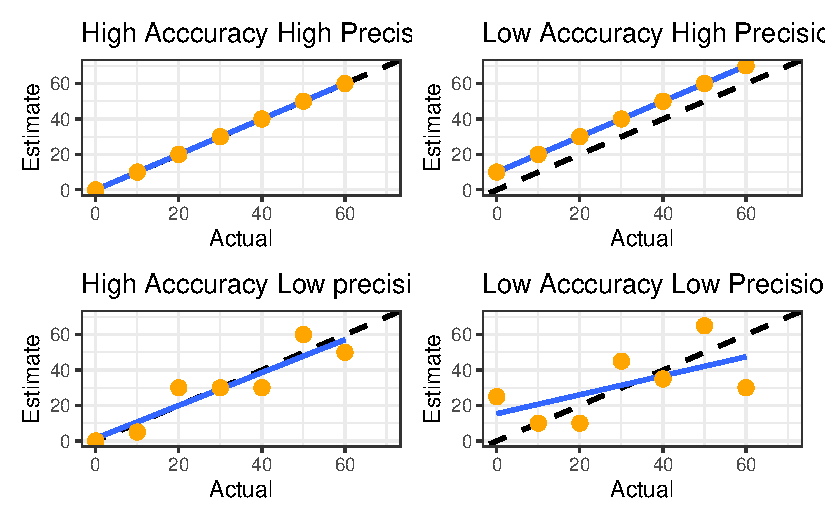
\includegraphics{./data-accuracy_files/figure-pdf/fig-accuracy-1.pdf}

}

\caption{\label{fig-accuracy}Scatter plots for the relationship between
actual and estimated values representing situations of low or high
precision and accuracy. The dashed line indicates the perfect
concordance and the solid blue line represents the fit of the linear
regression model}

\end{figure}

\hypertarget{statistical-summaries}{%
\section{Statistical summaries}\label{statistical-summaries}}

A formal assessment of the quality of estimates or measures is made
using statistical summaries of the data expressed as indices that
represent reliability, precision and accuracy. These indices can further
be used to test hypothesis such as if one or another method is superior
than the other. The indices or the tests vary according to the nature of
the variable, whether continuous, binary or categorical.

\hypertarget{inter-rater-reliability}{%
\subsection{Inter-rater reliability}\label{inter-rater-reliability}}

To calculate measures of inter-rater reliability (or reproducibility) we
will work with a fraction of a larger dataset used in a published
\href{https://bsppjournals.onlinelibrary.wiley.com/doi/abs/10.1111/ppa.13148}{study}.
There, the authors tested the effect of standard area diagrams (SADs) on
the reliability and accuracy of visual estimates of severity of soybean
rust.

The selected dataset consists of five columns with 20 rows. The first is
the leaf number and the others correspond to assessments of percent
soybean rust severity by four raters (R1 to R4). Each row correspond to
one symptomatic leaf. Let's assign the tibble to a dataframe called
\texttt{sbr} (an acronym for soybean rust). Note that the variable is
continuous.

\begin{Shaded}
\begin{Highlighting}[]
\FunctionTok{library}\NormalTok{(tidyverse)}
\NormalTok{sbr }\OtherTok{\textless{}{-}} \FunctionTok{tribble}\NormalTok{(}
\SpecialCharTok{\textasciitilde{}}\NormalTok{leaf, }\SpecialCharTok{\textasciitilde{}}\NormalTok{R1, }\SpecialCharTok{\textasciitilde{}}\NormalTok{R2,  }\SpecialCharTok{\textasciitilde{}}\NormalTok{R3, }\SpecialCharTok{\textasciitilde{}}\NormalTok{R4,}
\DecValTok{1}\NormalTok{, }\FloatTok{0.6}\NormalTok{, }\FloatTok{0.6}\NormalTok{,  }\FloatTok{0.7}\NormalTok{, }\FloatTok{0.6}\NormalTok{,}
\DecValTok{2}\NormalTok{,   }\DecValTok{2}\NormalTok{, }\FloatTok{0.7}\NormalTok{,    }\DecValTok{5}\NormalTok{,   }\DecValTok{1}\NormalTok{,}
\DecValTok{3}\NormalTok{,   }\DecValTok{5}\NormalTok{,   }\DecValTok{5}\NormalTok{,    }\DecValTok{8}\NormalTok{,   }\DecValTok{5}\NormalTok{,}
\DecValTok{4}\NormalTok{,   }\DecValTok{2}\NormalTok{,   }\DecValTok{4}\NormalTok{,    }\DecValTok{6}\NormalTok{,   }\DecValTok{2}\NormalTok{,}
\DecValTok{5}\NormalTok{,   }\DecValTok{6}\NormalTok{,  }\DecValTok{14}\NormalTok{,   }\DecValTok{10}\NormalTok{,   }\DecValTok{7}\NormalTok{,}
\DecValTok{6}\NormalTok{,   }\DecValTok{5}\NormalTok{,   }\DecValTok{6}\NormalTok{,   }\DecValTok{10}\NormalTok{,   }\DecValTok{5}\NormalTok{,}
\DecValTok{7}\NormalTok{,  }\DecValTok{10}\NormalTok{,  }\DecValTok{18}\NormalTok{, }\FloatTok{12.5}\NormalTok{,  }\DecValTok{12}\NormalTok{,}
\DecValTok{8}\NormalTok{,  }\DecValTok{15}\NormalTok{,  }\DecValTok{30}\NormalTok{,   }\DecValTok{22}\NormalTok{,  }\DecValTok{10}\NormalTok{,}
\DecValTok{9}\NormalTok{,   }\DecValTok{7}\NormalTok{,   }\DecValTok{2}\NormalTok{,   }\DecValTok{12}\NormalTok{,   }\DecValTok{8}\NormalTok{,}
\DecValTok{10}\NormalTok{,  }\DecValTok{6}\NormalTok{,   }\DecValTok{9}\NormalTok{, }\FloatTok{11.5}\NormalTok{,   }\DecValTok{8}\NormalTok{,}
\DecValTok{11}\NormalTok{,  }\DecValTok{7}\NormalTok{,   }\DecValTok{7}\NormalTok{,   }\DecValTok{20}\NormalTok{,   }\DecValTok{9}\NormalTok{,}
\DecValTok{12}\NormalTok{,  }\DecValTok{6}\NormalTok{,  }\DecValTok{23}\NormalTok{,   }\DecValTok{22}\NormalTok{,  }\DecValTok{14}\NormalTok{,}
\DecValTok{13}\NormalTok{, }\DecValTok{10}\NormalTok{,  }\DecValTok{35}\NormalTok{, }\FloatTok{18.5}\NormalTok{,  }\DecValTok{20}\NormalTok{,}
\DecValTok{14}\NormalTok{, }\DecValTok{19}\NormalTok{,  }\DecValTok{10}\NormalTok{,    }\DecValTok{9}\NormalTok{,  }\DecValTok{10}\NormalTok{,}
\DecValTok{15}\NormalTok{, }\DecValTok{15}\NormalTok{,  }\DecValTok{20}\NormalTok{,   }\DecValTok{19}\NormalTok{,  }\DecValTok{20}\NormalTok{,}
\DecValTok{16}\NormalTok{, }\DecValTok{17}\NormalTok{,  }\DecValTok{30}\NormalTok{,   }\DecValTok{18}\NormalTok{,  }\DecValTok{13}\NormalTok{,}
\DecValTok{17}\NormalTok{, }\DecValTok{19}\NormalTok{,  }\DecValTok{53}\NormalTok{,   }\DecValTok{33}\NormalTok{,  }\DecValTok{38}\NormalTok{,}
\DecValTok{18}\NormalTok{, }\DecValTok{17}\NormalTok{, }\FloatTok{6.8}\NormalTok{,   }\DecValTok{15}\NormalTok{,   }\DecValTok{9}\NormalTok{,}
\DecValTok{19}\NormalTok{, }\DecValTok{15}\NormalTok{,  }\DecValTok{20}\NormalTok{,   }\DecValTok{18}\NormalTok{,  }\DecValTok{16}\NormalTok{,}
\DecValTok{20}\NormalTok{, }\DecValTok{18}\NormalTok{,  }\DecValTok{22}\NormalTok{,   }\DecValTok{24}\NormalTok{,  }\DecValTok{15}
\NormalTok{         )}
\end{Highlighting}
\end{Shaded}

Let's explore the data using various approaches. First, we can visualize
how the individual estimates by the raters differ for a same leaf.

\begin{Shaded}
\begin{Highlighting}[]
\CommentTok{\# set the global theme}
\FunctionTok{theme\_set}\NormalTok{(}\FunctionTok{theme\_bw}\NormalTok{())}
\FunctionTok{library}\NormalTok{(ggthemes)}

\CommentTok{\# transform from wide to long format}
\NormalTok{sbr2 }\OtherTok{\textless{}{-}}\NormalTok{ sbr }\SpecialCharTok{|\textgreater{}} 
  \FunctionTok{pivot\_longer}\NormalTok{(}\DecValTok{2}\SpecialCharTok{:}\DecValTok{5}\NormalTok{, }\AttributeTok{names\_to =} \StringTok{"rater"}\NormalTok{,}
               \AttributeTok{values\_to =} \StringTok{"estimate"}\NormalTok{) }

\CommentTok{\# create the plot}
\NormalTok{sbr2 }\SpecialCharTok{|\textgreater{}} 
  \FunctionTok{ggplot}\NormalTok{(}\FunctionTok{aes}\NormalTok{(leaf, estimate, }\AttributeTok{color =}\NormalTok{ rater,}
             \AttributeTok{group =}\NormalTok{ leaf))}\SpecialCharTok{+}
  \FunctionTok{geom\_line}\NormalTok{(}\AttributeTok{color =} \StringTok{"black"}\NormalTok{)}\SpecialCharTok{+}
  \FunctionTok{geom\_point}\NormalTok{(}\AttributeTok{size =} \DecValTok{2}\NormalTok{)}\SpecialCharTok{+}
  \FunctionTok{scale\_color\_colorblind}\NormalTok{()}\SpecialCharTok{+}
  \FunctionTok{labs}\NormalTok{(}\AttributeTok{y =} \StringTok{"Severity estimate (\%)"}\NormalTok{,}
       \AttributeTok{x =} \StringTok{"Leaf number"}\NormalTok{,}
       \AttributeTok{color =} \StringTok{"Rater"}\NormalTok{)}
\end{Highlighting}
\end{Shaded}

\begin{figure}[H]

{\centering 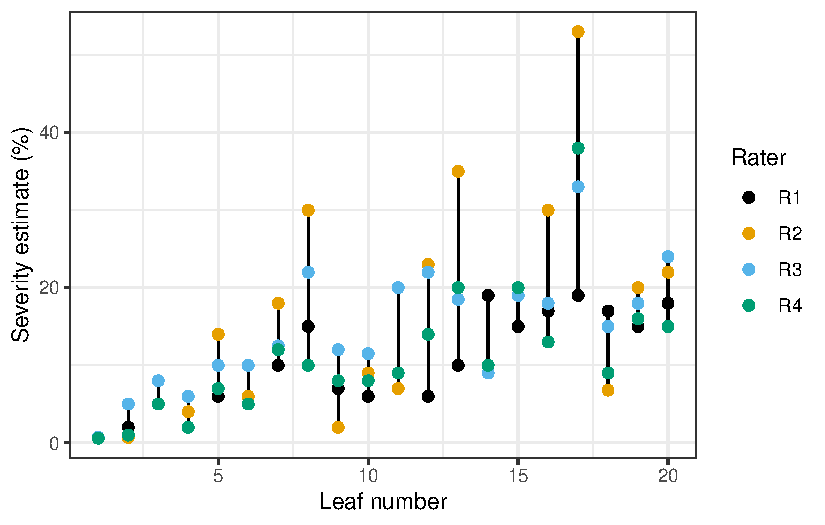
\includegraphics{./data-accuracy_files/figure-pdf/fig-raters1-1.pdf}

}

\caption{\label{fig-raters1}Visual estimates of soybean rust severity
for each leaf by each of four raters}

\end{figure}

Alternatively, we can visualize the distribution of the estimates by
rater using boxplots.

\begin{Shaded}
\begin{Highlighting}[]
\NormalTok{sbr2 }\SpecialCharTok{|\textgreater{}} 
  \FunctionTok{ggplot}\NormalTok{(}\FunctionTok{aes}\NormalTok{(rater, estimate))}\SpecialCharTok{+}
  \FunctionTok{geom\_boxplot}\NormalTok{(}\AttributeTok{outlier.colour =} \ConstantTok{NA}\NormalTok{, }\AttributeTok{width =}\FloatTok{0.5}\NormalTok{)}\SpecialCharTok{+}
  \FunctionTok{geom\_jitter}\NormalTok{(}\AttributeTok{width =} \FloatTok{0.1}\NormalTok{,}\AttributeTok{shape =} \DecValTok{1}\NormalTok{, }\AttributeTok{size =}\DecValTok{2}\NormalTok{)}\SpecialCharTok{+}
  \FunctionTok{labs}\NormalTok{(}\AttributeTok{y =} \StringTok{"Severity estimate (\%)"}\NormalTok{,}
       \AttributeTok{x =} \StringTok{"Rater"}\NormalTok{)}
\end{Highlighting}
\end{Shaded}

\begin{figure}[H]

{\centering 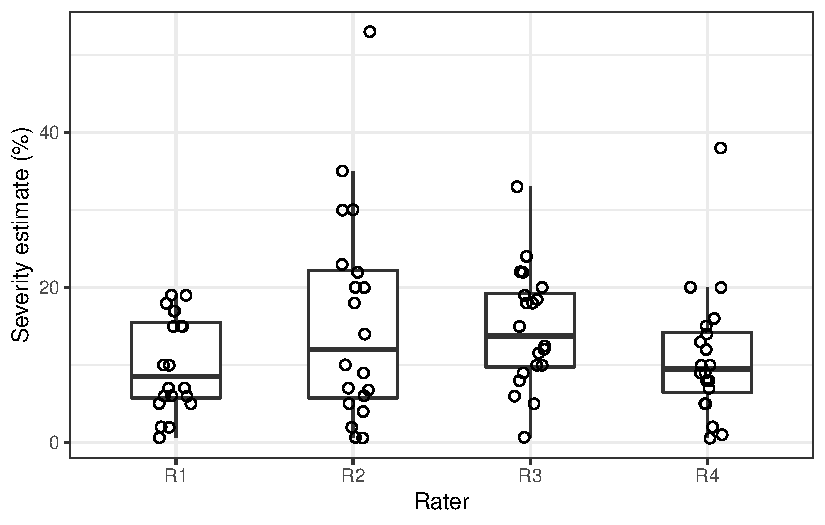
\includegraphics{./data-accuracy_files/figure-pdf/fig-raters2-1.pdf}

}

\caption{\label{fig-raters2}Distribution of severity estimates of
soybean rust by rater}

\end{figure}

Another interesting visualization is the correlation matrix of the
estimates between all possible pair of raters. The \texttt{ggpairs}
function of the \emph{GGally} package is handy for this task.

\begin{Shaded}
\begin{Highlighting}[]
\FunctionTok{library}\NormalTok{(GGally)}
\FunctionTok{theme\_set}\NormalTok{(}\FunctionTok{theme\_light}\NormalTok{())}

\CommentTok{\# create a new dataframe with only raters}
\NormalTok{raters }\OtherTok{\textless{}{-}}\NormalTok{ sbr }\SpecialCharTok{|\textgreater{}} 
  \FunctionTok{select}\NormalTok{(}\DecValTok{2}\SpecialCharTok{:}\DecValTok{5}\NormalTok{)}

\FunctionTok{ggpairs}\NormalTok{(raters)}
\end{Highlighting}
\end{Shaded}

\begin{figure}[H]

{\centering 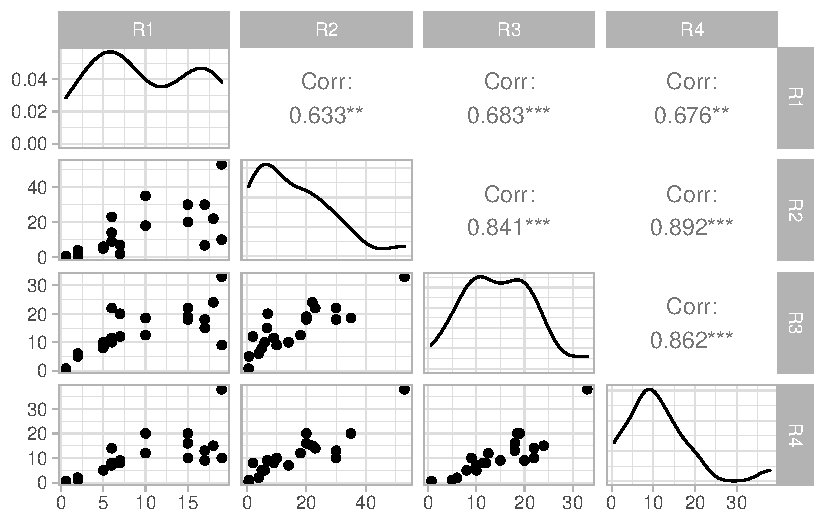
\includegraphics{./data-accuracy_files/figure-pdf/fig-correl-1.pdf}

}

\caption{\label{fig-correl}Correlation plots relating severity estimates
for all pairs of raters}

\end{figure}

\hypertarget{coefficient-of-determination}{%
\subsubsection{Coefficient of
determination}\label{coefficient-of-determination}}

We noticed earlier that the correlation coefficients varied across all
pairs of rater. Sometimes, the means of squared Pearson's R values (R2),
or the coefficient of determination is used as a measure of inter-rater
reliability. We can further examine the pair-wise correlations in more
details using the \texttt{correlation} function of the
\emph{performance} package.

\begin{Shaded}
\begin{Highlighting}[]
\FunctionTok{library}\NormalTok{(correlation)}
\NormalTok{raters\_cor }\OtherTok{\textless{}{-}} \FunctionTok{correlation}\NormalTok{(raters)}
\FunctionTok{library}\NormalTok{(knitr)}
\FunctionTok{kable}\NormalTok{(raters\_cor[}\DecValTok{1}\SpecialCharTok{:}\DecValTok{3}\NormalTok{]) }\CommentTok{\# only first 3 variables}
\end{Highlighting}
\end{Shaded}

\hypertarget{tbl-correl}{}
\begin{longtable}[]{@{}llr@{}}
\caption{\label{tbl-correl}Pearson correlation coefficients for all
pairs of raters}\tabularnewline
\toprule()
Parameter1 & Parameter2 & r \\
\midrule()
\endfirsthead
\toprule()
Parameter1 & Parameter2 & r \\
\midrule()
\endhead
R1 & R2 & 0.6325037 \\
R1 & R3 & 0.6825936 \\
R1 & R4 & 0.6756986 \\
R2 & R3 & 0.8413333 \\
R2 & R4 & 0.8922181 \\
R3 & R4 & 0.8615470 \\
\bottomrule()
\end{longtable}

The means of coefficient of determination can be easily obtained as
follows.

\begin{Shaded}
\begin{Highlighting}[]
\CommentTok{\# All pairwise R2}
\FunctionTok{round}\NormalTok{(raters\_cor}\SpecialCharTok{$}\NormalTok{r}\SpecialCharTok{\^{}}\DecValTok{2}\NormalTok{,}\DecValTok{2}\NormalTok{)}
\end{Highlighting}
\end{Shaded}

\begin{verbatim}
[1] 0.40 0.47 0.46 0.71 0.80 0.74
\end{verbatim}

\begin{Shaded}
\begin{Highlighting}[]
\CommentTok{\# means of R2}
\FunctionTok{round}\NormalTok{(}\FunctionTok{mean}\NormalTok{(raters\_cor}\SpecialCharTok{$}\NormalTok{r}\SpecialCharTok{\^{}}\DecValTok{2}\NormalTok{), }\DecValTok{2}\NormalTok{)}
\end{Highlighting}
\end{Shaded}

\begin{verbatim}
[1] 0.59
\end{verbatim}

\hypertarget{intraclass-correlation-coefficient}{%
\subsubsection{Intraclass Correlation
Coefficient}\label{intraclass-correlation-coefficient}}

A common statistic to report in reliability studies is the Intraclass
Correlation Coefficient (ICC). There are several formulations for the
ICC whose choice depend on the particular experimental design. Following
the convention of the seminal work by Shrout and Fleiss (1979), there
are three main ICCs:

\begin{itemize}
\item
  One-way random effects model, ICC(1,1): in our context, each leaf is
  rated by different raters who are considered as sampled from a larger
  pool of raters (random effects)
\item
  Two-way random effects model, ICC(2,1): both raters and leaves are
  viewed as random effects
\item
  Two-way mixed model, ICC(3,1): raters are considered as fixed effects
  and leaves are considered as random.
\end{itemize}

Additionally, the ICC may depend on whether the ratings are an average
or not of several ratings. When an average is considered, these are
called ICC(1,k), ICC(2,k) and ICC(3,k).

The ICC can be computed using the \texttt{ICC()} or the \texttt{icc()}
functions of the \emph{psych} or \emph{irr} packages, respectively. They
both provide the coefficient, F value, and the upper and lower bounds of
the 95\% confidence interval.

\begin{Shaded}
\begin{Highlighting}[]
\FunctionTok{library}\NormalTok{(psych)}
\NormalTok{ic }\OtherTok{\textless{}{-}} \FunctionTok{ICC}\NormalTok{(raters)}
\FunctionTok{kable}\NormalTok{(ic}\SpecialCharTok{$}\NormalTok{results[}\DecValTok{1}\SpecialCharTok{:}\DecValTok{2}\NormalTok{]) }\CommentTok{\# only selected columns}
\end{Highlighting}
\end{Shaded}

\begin{longtable}[]{@{}llr@{}}
\toprule()
& type & ICC \\
\midrule()
\endhead
Single\_raters\_absolute & ICC1 & 0.6405024 \\
Single\_random\_raters & ICC2 & 0.6464122 \\
Single\_fixed\_raters & ICC3 & 0.6919099 \\
Average\_raters\_absolute & ICC1k & 0.8769479 \\
Average\_random\_raters & ICC2k & 0.8797008 \\
Average\_fixed\_raters & ICC3k & 0.8998319 \\
\bottomrule()
\end{longtable}

\begin{Shaded}
\begin{Highlighting}[]
\CommentTok{\# call ic list for full results}
\end{Highlighting}
\end{Shaded}

The output of interest is a dataframe with the results of all distinct
ICCs. We note that the ICC1 and ICC2 gave very close results. Now, let's
obtain the various ICCs using the \emph{irr} package. Differently from
the the \texttt{ICC()} function, this one requires further specification
of the model to use.

\begin{Shaded}
\begin{Highlighting}[]
\FunctionTok{library}\NormalTok{(irr)}
\FunctionTok{icc}\NormalTok{(raters, }\StringTok{"oneway"}\NormalTok{)}
\end{Highlighting}
\end{Shaded}

\begin{verbatim}
 Single Score Intraclass Correlation

   Model: oneway 
   Type : consistency 

   Subjects = 20 
     Raters = 4 
     ICC(1) = 0.641

 F-Test, H0: r0 = 0 ; H1: r0 > 0 
   F(19,60) = 8.13 , p = 1.8e-10 

 95%-Confidence Interval for ICC Population Values:
  0.44 < ICC < 0.813
\end{verbatim}

\begin{Shaded}
\begin{Highlighting}[]
\CommentTok{\# The one used in the SBR paper}
\FunctionTok{icc}\NormalTok{(raters, }\StringTok{"twoway"}\NormalTok{)}
\end{Highlighting}
\end{Shaded}

\begin{verbatim}
 Single Score Intraclass Correlation

   Model: twoway 
   Type : consistency 

   Subjects = 20 
     Raters = 4 
   ICC(C,1) = 0.692

 F-Test, H0: r0 = 0 ; H1: r0 > 0 
   F(19,57) = 9.98 , p = 6.08e-12 

 95%-Confidence Interval for ICC Population Values:
  0.503 < ICC < 0.845
\end{verbatim}

\hypertarget{overall-concordance-correlation-coefficient}{%
\subsubsection{Overall Concordance Correlation
Coefficient}\label{overall-concordance-correlation-coefficient}}

Another useful index is the Overall Concordance Correlation Coefficient
(OCCC) for evaluating agreement among multiple observers. It was
proposed by Barnhart et al. (2002) based on the original index proposed
by Lin (1989), earlier defined in the context of two fixed observers. In
the paper, the authors introduced the OCCC in terms of the interobserver
variability for assessing agreement among multiple fixed observers. As
outcome, and similar to the original CCC, the approach addresses the
precision and accuracy indices as components of the OCCC. The
\texttt{epi.occc} function of the \emph{epiR} packge does the job but it
does compute a confidence interval.

\begin{Shaded}
\begin{Highlighting}[]
\FunctionTok{library}\NormalTok{(epiR)}
\FunctionTok{epi.occc}\NormalTok{(raters, }\AttributeTok{na.rm =} \ConstantTok{FALSE}\NormalTok{, }\AttributeTok{pairs =} \ConstantTok{TRUE}\NormalTok{)}
\end{Highlighting}
\end{Shaded}

\begin{verbatim}

Overall CCC           0.6372
Overall precision     0.7843
Overall accuracy      0.8125
\end{verbatim}

\hypertarget{intrarater-reliability}{%
\subsection{Intrarater reliability}\label{intrarater-reliability}}

As defined, the intrarater reliability is also known as repeatability,
because it measures consistency by the same rater at repeated
assessments (e.g.~different times) on the same sample. In some studies,
we may be interested in testing whether a new method increases
repeatability of assessments by a single rater compared with another
one. The same indices used for assessing reproducibility (interrater)
can be used to assess repeatability, and these are reported at the rater
level.

\hypertarget{precision}{%
\subsection{Precision}\label{precision}}

When assessing precision, one measures the variability of the estimates
(or measurements) of disease on the same sampling units obtained by
different raters (or instruments). A very high precision does not mean
that the estimates are closer to the actual value (which is given by
measures of bias). However, precision is a component of overall
accuracy, or agreement. It is given by the Pearson's correlation
coefficient.

Different from reliability, that requires only the estimates or measures
by the raters, now we need a reference (gold standard) value to compare
the estimates to. These can be an accurate rater or measures by an
instrument. Let's get back to the soybean rust severity estimation
dataset and add a column for the (assumed) actual values of severity on
each leaf. In that work, the actual severity values were obtained using
image analysis.

\begin{Shaded}
\begin{Highlighting}[]
\NormalTok{sbr }\OtherTok{\textless{}{-}}\NormalTok{ tibble}\SpecialCharTok{::}\FunctionTok{tribble}\NormalTok{(}
\SpecialCharTok{\textasciitilde{}}\NormalTok{leaf, }\SpecialCharTok{\textasciitilde{}}\NormalTok{actual, }\SpecialCharTok{\textasciitilde{}}\NormalTok{R1, }\SpecialCharTok{\textasciitilde{}}\NormalTok{R2,  }\SpecialCharTok{\textasciitilde{}}\NormalTok{R3, }\SpecialCharTok{\textasciitilde{}}\NormalTok{R4,}
\DecValTok{1}\NormalTok{,    }\FloatTok{0.25}\NormalTok{, }\FloatTok{0.6}\NormalTok{, }\FloatTok{0.6}\NormalTok{,  }\FloatTok{0.7}\NormalTok{, }\FloatTok{0.6}\NormalTok{,}
\DecValTok{2}\NormalTok{,     }\FloatTok{2.5}\NormalTok{,   }\DecValTok{2}\NormalTok{, }\FloatTok{0.7}\NormalTok{,    }\DecValTok{5}\NormalTok{,   }\DecValTok{1}\NormalTok{,}
\DecValTok{3}\NormalTok{,    }\FloatTok{7.24}\NormalTok{,   }\DecValTok{5}\NormalTok{,   }\DecValTok{5}\NormalTok{,    }\DecValTok{8}\NormalTok{,   }\DecValTok{5}\NormalTok{,}
\DecValTok{4}\NormalTok{,    }\FloatTok{7.31}\NormalTok{,   }\DecValTok{2}\NormalTok{,   }\DecValTok{4}\NormalTok{,    }\DecValTok{6}\NormalTok{,   }\DecValTok{2}\NormalTok{,}
\DecValTok{5}\NormalTok{,    }\FloatTok{9.07}\NormalTok{,   }\DecValTok{6}\NormalTok{,  }\DecValTok{14}\NormalTok{,   }\DecValTok{10}\NormalTok{,   }\DecValTok{7}\NormalTok{,}
\DecValTok{6}\NormalTok{,    }\FloatTok{11.6}\NormalTok{,   }\DecValTok{5}\NormalTok{,   }\DecValTok{6}\NormalTok{,   }\DecValTok{10}\NormalTok{,   }\DecValTok{5}\NormalTok{,}
\DecValTok{7}\NormalTok{,   }\FloatTok{12.46}\NormalTok{,  }\DecValTok{10}\NormalTok{,  }\DecValTok{18}\NormalTok{, }\FloatTok{12.5}\NormalTok{,  }\DecValTok{12}\NormalTok{,}
\DecValTok{8}\NormalTok{,    }\FloatTok{13.1}\NormalTok{,  }\DecValTok{15}\NormalTok{,  }\DecValTok{30}\NormalTok{,   }\DecValTok{22}\NormalTok{,  }\DecValTok{10}\NormalTok{,}
\DecValTok{9}\NormalTok{,   }\FloatTok{14.61}\NormalTok{,   }\DecValTok{7}\NormalTok{,   }\DecValTok{2}\NormalTok{,   }\DecValTok{12}\NormalTok{,   }\DecValTok{8}\NormalTok{,}
\DecValTok{10}\NormalTok{,  }\FloatTok{16.06}\NormalTok{,   }\DecValTok{6}\NormalTok{,   }\DecValTok{9}\NormalTok{, }\FloatTok{11.5}\NormalTok{,   }\DecValTok{8}\NormalTok{,}
\DecValTok{11}\NormalTok{,   }\FloatTok{16.7}\NormalTok{,   }\DecValTok{7}\NormalTok{,   }\DecValTok{7}\NormalTok{,   }\DecValTok{20}\NormalTok{,   }\DecValTok{9}\NormalTok{,}
\DecValTok{12}\NormalTok{,   }\FloatTok{19.5}\NormalTok{,   }\DecValTok{6}\NormalTok{,  }\DecValTok{23}\NormalTok{,   }\DecValTok{22}\NormalTok{,  }\DecValTok{14}\NormalTok{,}
\DecValTok{13}\NormalTok{,  }\FloatTok{20.75}\NormalTok{,  }\DecValTok{10}\NormalTok{,  }\DecValTok{35}\NormalTok{, }\FloatTok{18.5}\NormalTok{,  }\DecValTok{20}\NormalTok{,}
\DecValTok{14}\NormalTok{,  }\FloatTok{23.56}\NormalTok{,  }\DecValTok{19}\NormalTok{,  }\DecValTok{10}\NormalTok{,    }\DecValTok{9}\NormalTok{,  }\DecValTok{10}\NormalTok{,}
\DecValTok{15}\NormalTok{,  }\FloatTok{23.77}\NormalTok{,  }\DecValTok{15}\NormalTok{,  }\DecValTok{20}\NormalTok{,   }\DecValTok{19}\NormalTok{,  }\DecValTok{20}\NormalTok{,}
\DecValTok{16}\NormalTok{,  }\FloatTok{24.45}\NormalTok{,  }\DecValTok{17}\NormalTok{,  }\DecValTok{30}\NormalTok{,   }\DecValTok{18}\NormalTok{,  }\DecValTok{13}\NormalTok{,}
\DecValTok{17}\NormalTok{,  }\FloatTok{25.78}\NormalTok{,  }\DecValTok{19}\NormalTok{,  }\DecValTok{53}\NormalTok{,   }\DecValTok{33}\NormalTok{,  }\DecValTok{38}\NormalTok{,}
\DecValTok{18}\NormalTok{,  }\FloatTok{26.03}\NormalTok{,  }\DecValTok{17}\NormalTok{, }\FloatTok{6.8}\NormalTok{,   }\DecValTok{15}\NormalTok{,   }\DecValTok{9}\NormalTok{,}
\DecValTok{19}\NormalTok{,  }\FloatTok{26.42}\NormalTok{,  }\DecValTok{15}\NormalTok{,  }\DecValTok{20}\NormalTok{,   }\DecValTok{18}\NormalTok{,  }\DecValTok{16}\NormalTok{,}
\DecValTok{20}\NormalTok{,  }\FloatTok{28.89}\NormalTok{,  }\DecValTok{18}\NormalTok{,  }\DecValTok{22}\NormalTok{,   }\DecValTok{24}\NormalTok{,  }\DecValTok{15}
\NormalTok{         )}
\end{Highlighting}
\end{Shaded}

We can explore visually via scatter plots the relationships between the
actual value and the estimates by each rater (Figure~\ref{fig-scater}).
To facilitate, we need the data in the long format.

\begin{Shaded}
\begin{Highlighting}[]
\NormalTok{sbr2 }\OtherTok{\textless{}{-}}\NormalTok{ sbr }\SpecialCharTok{|\textgreater{}} 
  \FunctionTok{pivot\_longer}\NormalTok{(}\DecValTok{3}\SpecialCharTok{:}\DecValTok{6}\NormalTok{, }\AttributeTok{names\_to =} \StringTok{"rater"}\NormalTok{,}
               \AttributeTok{values\_to =} \StringTok{"estimate"}\NormalTok{) }

\NormalTok{sbr2 }\SpecialCharTok{|\textgreater{}} 
  \FunctionTok{ggplot}\NormalTok{(}\FunctionTok{aes}\NormalTok{(actual, estimate))}\SpecialCharTok{+}
  \FunctionTok{geom\_point}\NormalTok{(}\AttributeTok{size =} \DecValTok{2}\NormalTok{, }\AttributeTok{alpha =} \FloatTok{0.7}\NormalTok{)}\SpecialCharTok{+}
  \FunctionTok{facet\_wrap}\NormalTok{(}\SpecialCharTok{\textasciitilde{}}\NormalTok{rater)}\SpecialCharTok{+}
  \FunctionTok{ylim}\NormalTok{(}\DecValTok{0}\NormalTok{,}\DecValTok{45}\NormalTok{)}\SpecialCharTok{+}
  \FunctionTok{xlim}\NormalTok{(}\DecValTok{0}\NormalTok{,}\DecValTok{45}\NormalTok{)}\SpecialCharTok{+}
  \FunctionTok{geom\_abline}\NormalTok{(}\AttributeTok{intercept =} \DecValTok{0}\NormalTok{, }\AttributeTok{slope =}\DecValTok{1}\NormalTok{)}\SpecialCharTok{+}
  \FunctionTok{labs}\NormalTok{(}\AttributeTok{x =} \StringTok{"Actual severity (\%)"}\NormalTok{,}
       \AttributeTok{y =} \StringTok{"Estimate severity (\%)"}\NormalTok{)}
\end{Highlighting}
\end{Shaded}

\begin{figure}[H]

{\centering 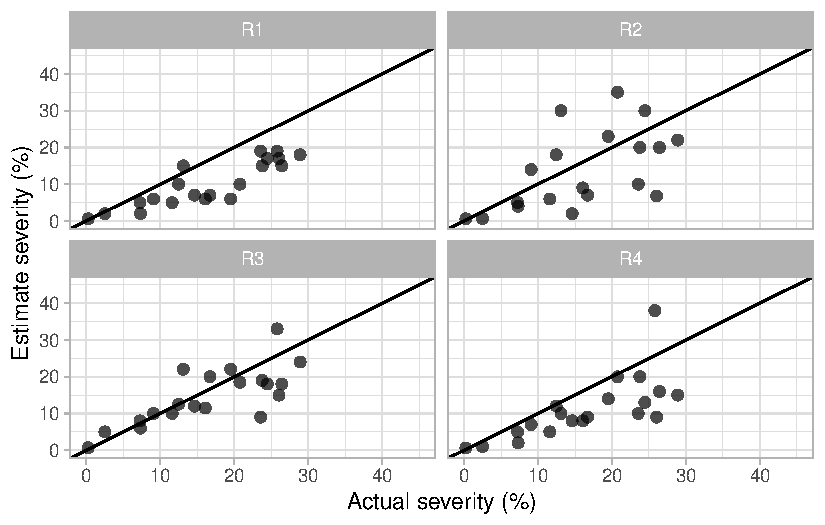
\includegraphics{./data-accuracy_files/figure-pdf/fig-scater-1.pdf}

}

\caption{\label{fig-scater}Scatterplots for the relationship between
estimated and actual severity for each rater}

\end{figure}

The Pearson's r for the relationship, or the precision of the estimates
by each rater, can be obtained using the \texttt{correlation} function
of the \emph{correlation} package.

\begin{Shaded}
\begin{Highlighting}[]
\NormalTok{precision }\OtherTok{\textless{}{-}}\NormalTok{ sbr2 }\SpecialCharTok{|\textgreater{}} 
  \FunctionTok{select}\NormalTok{(}\SpecialCharTok{{-}}\NormalTok{leaf) }\SpecialCharTok{|\textgreater{}} 
  \FunctionTok{group\_by}\NormalTok{(rater) }\SpecialCharTok{|\textgreater{}} 
  \FunctionTok{correlation}\NormalTok{() }

\FunctionTok{kable}\NormalTok{(precision[}\DecValTok{1}\SpecialCharTok{:}\DecValTok{4}\NormalTok{])}
\end{Highlighting}
\end{Shaded}

\begin{longtable}[]{@{}lllr@{}}
\toprule()
Group & Parameter1 & Parameter2 & r \\
\midrule()
\endhead
R1 & actual & estimate & 0.8725643 \\
R2 & actual & estimate & 0.5845291 \\
R3 & actual & estimate & 0.7531983 \\
R4 & actual & estimate & 0.7108260 \\
\bottomrule()
\end{longtable}

The mean precision can then be obtained.

\begin{Shaded}
\begin{Highlighting}[]
\FunctionTok{mean}\NormalTok{(precision}\SpecialCharTok{$}\NormalTok{r)}
\end{Highlighting}
\end{Shaded}

\begin{verbatim}
[1] 0.7302795
\end{verbatim}

\hypertarget{accuracy}{%
\subsection{Accuracy}\label{accuracy}}

\hypertarget{absolute-errors}{%
\subsubsection{Absolute errors}\label{absolute-errors}}

It is useful to visualize the errors of the estimates which are obtained
by subtracting the estimates from the actual severity values. This plot
allows to visualize patterns in over or underestimations across a range
of actual severity values.

\begin{Shaded}
\begin{Highlighting}[]
\NormalTok{sbr2 }\SpecialCharTok{|\textgreater{}} 
  \FunctionTok{ggplot}\NormalTok{(}\FunctionTok{aes}\NormalTok{(actual, estimate}\SpecialCharTok{{-}}\NormalTok{actual))}\SpecialCharTok{+}
  \FunctionTok{geom\_point}\NormalTok{(}\AttributeTok{size =} \DecValTok{3}\NormalTok{, }\AttributeTok{alpha =} \FloatTok{0.7}\NormalTok{)}\SpecialCharTok{+}
  \FunctionTok{facet\_wrap}\NormalTok{(}\SpecialCharTok{\textasciitilde{}}\NormalTok{rater)}\SpecialCharTok{+}
  \FunctionTok{geom\_hline}\NormalTok{(}\AttributeTok{yintercept =} \DecValTok{0}\NormalTok{)}\SpecialCharTok{+}
  \FunctionTok{labs}\NormalTok{(}\AttributeTok{x =} \StringTok{"Actual severity (\%)"}\NormalTok{,}
       \AttributeTok{y =} \StringTok{"Error (Estimate {-} Actual)"}\NormalTok{)}
\end{Highlighting}
\end{Shaded}

\begin{figure}[H]

{\centering 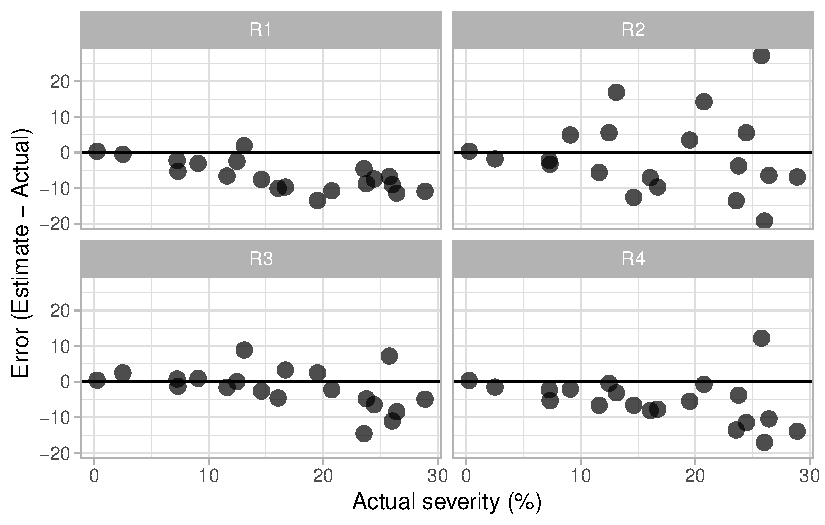
\includegraphics{./data-accuracy_files/figure-pdf/fig-errors-1.pdf}

}

\caption{\label{fig-errors}Error (estimated - actual) of visual severity
estimates}

\end{figure}

\hypertarget{concordance-correlation-coefficient}{%
\subsubsection{Concordance correlation
coefficient}\label{concordance-correlation-coefficient}}

Lin's (1989, 2000) proposed the concordance correlation coefficient
(CCC) for agreement on a continuous measure obtained by two methods. The
CCC combines measures of both precision and accuracy to determine how
far the observed data deviate from the line of perfect concordance.
Lin's CCC increases in value as a function of the nearness of the data
reduced major axis to the line of perfect concordance (the accuracy of
the data) and of the tightness of the data about its reduced major axis
(the precision of the data).

The \texttt{epi.ccc} function of the \emph{epiR} package allows to
obtain the Lin's CCC statistics. Let's filter only rater 2 and calculate
the CCC statistics for this rater.

\begin{Shaded}
\begin{Highlighting}[]
\FunctionTok{library}\NormalTok{(epiR)}
\CommentTok{\# Only rater 2}
\NormalTok{sbr3 }\OtherTok{\textless{}{-}}\NormalTok{ sbr2 }\SpecialCharTok{|\textgreater{}} \FunctionTok{filter}\NormalTok{(rater }\SpecialCharTok{==} \StringTok{"R2"}\NormalTok{)}
\NormalTok{ccc }\OtherTok{\textless{}{-}} \FunctionTok{epi.ccc}\NormalTok{(sbr3}\SpecialCharTok{$}\NormalTok{actual, sbr3}\SpecialCharTok{$}\NormalTok{estimate)}
\CommentTok{\# Concordance coefficient}
\NormalTok{rho }\OtherTok{\textless{}{-}}\NormalTok{ ccc}\SpecialCharTok{$}\NormalTok{rho.c[,}\DecValTok{1}\NormalTok{]}
\CommentTok{\# Bias coefficient}
\NormalTok{Cb }\OtherTok{\textless{}{-}}\NormalTok{ ccc}\SpecialCharTok{$}\NormalTok{C.b}
\CommentTok{\# Precision}
\NormalTok{r }\OtherTok{\textless{}{-}}\NormalTok{ ccc}\SpecialCharTok{$}\NormalTok{C.b}\SpecialCharTok{*}\NormalTok{ccc}\SpecialCharTok{$}\NormalTok{rho.c[,}\DecValTok{1}\NormalTok{]}
\CommentTok{\# Scale{-}shift}
\NormalTok{ss }\OtherTok{\textless{}{-}}\NormalTok{ ccc}\SpecialCharTok{$}\NormalTok{s.shift}
\CommentTok{\# Location{-}shift}
\NormalTok{ls }\OtherTok{\textless{}{-}}\NormalTok{ ccc}\SpecialCharTok{$}\NormalTok{l.shift}
\NormalTok{Metrics }\OtherTok{\textless{}{-}} \FunctionTok{c}\NormalTok{(}\StringTok{"Agreement"}\NormalTok{, }\StringTok{"Bias coefficient"}\NormalTok{, }\StringTok{"Precision"}\NormalTok{, }\StringTok{"scale{-}shift"}\NormalTok{, }\StringTok{"location{-}shift"}\NormalTok{)}
\NormalTok{Value }\OtherTok{\textless{}{-}} \FunctionTok{c}\NormalTok{(rho, Cb, r, ss, ls)}
\NormalTok{res }\OtherTok{\textless{}{-}} \FunctionTok{data.frame}\NormalTok{(Metrics, Value)}
\FunctionTok{kable}\NormalTok{(res)}
\end{Highlighting}
\end{Shaded}

\hypertarget{tbl-ccc}{}
\begin{longtable}[]{@{}lr@{}}
\caption{\label{tbl-ccc}Statitics of the concordance correlation
coefficient summarizing accuracy and precision of visual severity
estimates of soybean rust for four raters}\tabularnewline
\toprule()
Metrics & Value \\
\midrule()
\endfirsthead
\toprule()
Metrics & Value \\
\midrule()
\endhead
Agreement & 0.5230656 \\
Bias coefficient & 0.8948494 \\
Precision & 0.4680649 \\
scale-shift & 1.6091178 \\
location-shift & -0.0666069 \\
\bottomrule()
\end{longtable}

\hypertarget{measuring-severity}{%
\chapter{Measuring severity}\label{measuring-severity}}

\begin{tcolorbox}[enhanced jigsaw, rightrule=.15mm, left=2mm, breakable, colframe=quarto-callout-note-color-frame, toprule=.15mm, leftrule=.75mm, bottomrule=.15mm, colback=white, arc=.35mm, opacityback=0]
\begin{minipage}[t]{5.5mm}
\textcolor{quarto-callout-note-color}{\faInfo}
\end{minipage}%
\begin{minipage}[t]{\textwidth - 5.5mm}
This is a work in progress that is currently undergoing heavy technical
editing and copy-editing\end{minipage}%
\end{tcolorbox}

\begin{tcolorbox}[enhanced jigsaw, rightrule=.15mm, left=2mm, breakable, colframe=quarto-callout-important-color-frame, toprule=.15mm, leftrule=.75mm, bottomrule=.15mm, colback=white, arc=.35mm, opacityback=0]
\begin{minipage}[t]{5.5mm}
\textcolor{quarto-callout-important-color}{\faExclamation}
\end{minipage}%
\begin{minipage}[t]{\textwidth - 5.5mm}
This chapter is adapted from a post published in
\href{https://openplantpathology.org/posts/2021-05-31-measuring-plant-disease-severity-using-the-pliman-r-package/}{Open
Plant Pathology}\end{minipage}%
\end{tcolorbox}

Among the different ways to express plant disease severity, the percent
area affected (symptomatic) by the disease is one of the most common
especially when dealing with diseases that affect leaves. To evaluate
whether the visual estimates of plant disease severity are sufficiently
accurate (as seen in the previous chapter), one needs the actual
severity values. These are also needed when preparing standard area
diagrams (SADs) which are diagrammatic representations of severity
values used as an aid prior or during the visual assessment to
standardize and produce more accurate results across different raters
(Del Ponte et al. 2017).

The actual severity values are usually approximated using image analysis
where the image is segmented and each pixel of the image is labeled
according to three different classes:

\begin{enumerate}
\def\labelenumi{\arabic{enumi}.}
\tightlist
\item
  Diseased (or symptomatic)
\item
  Non-diseased (or healthy)
\item
  Background (the non-plant portion of the image)
\end{enumerate}

The ratio between the diseased area and total area of the unit (e.g.~the
whole plant organ or section image) gives the proportion of diseased
area or the percent area affected (when multiplied by 100). Several
different proprietary or open-source software has been used by
researchers to determine the actual severity according to a review on
standard area diagrams (Del Ponte et al. 2017).

Here, we will use the \texttt{measure\_disease} function of the
\emph{pliman} (Plant IMage ANalysis) (Olivoto 2022) R package to obtain
measures of severity. The package was compared with other software for
determining plant disease severity on five different plant diseases and
showed to produce concordant results for most of the cases (Olivoto et
al. 2022).

There are basically two methods to measure severity. The first is based
on image palettes that define each class of the image. The second is
based on RGB-based indices (Alves et al. 2021).

\hypertarget{image-palettes}{%
\section{Image palettes}\label{image-palettes}}

The most critical is the initial step, when the user needs to correctly
define the color palettes. In \emph{pliman} the palettes are actually
separate images representing each of three classes named background (b),
symptomatic (s) and healthy (h).

The reference image palettes can be constructed by manually sampling
small areas of the image and producing a composite image. Of course, the
results may vary depending on how these areas are chosen. A work on the
validation of the \emph{pliman} to determine disease severity showed the
effect of different palettes prepared independently by three researchers
(Olivoto et al. 2022). The observation of the processed masks during the
calibration of the palettes is important to create reference palettes
that are most representative of the respective class.

Here, I cut and pasted several sections of images representative of each
class from a few leaves into a Google slide. Once the image palette was
ready, I exported each one as a separate image PNG file (JPG also
works). These were named: sbr\_b.png, sbr\_h.png and sbr\_s.png. They
can be found
\href{https://github.com/emdelponte/epidemiology-R/tree/main/imgs}{here
in this folder} for downloading.

\begin{figure}

{\centering 

\href{Fig_palettes}{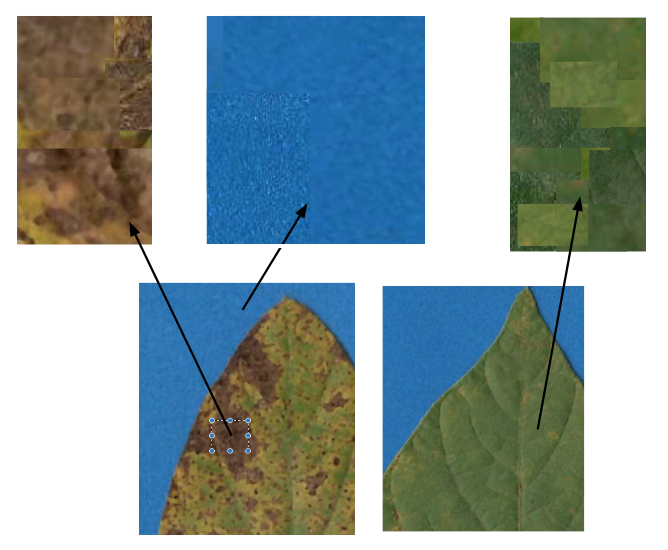
\includegraphics{./imgs/pliman1.png}}

}

\caption{Preparation of image palettes by manually sampling fraction of
the images that represent background, heatlhy leaf and lesions}

\end{figure}

Now that we have the image palettes, we can start by importing them into
the environment for further analysis. Let's create an image object for
each palette named h (healthy), s (symptoms) and b (background).

\begin{Shaded}
\begin{Highlighting}[]
\FunctionTok{library}\NormalTok{(pliman)}
\NormalTok{h }\OtherTok{\textless{}{-}} \FunctionTok{image\_import}\NormalTok{(}\StringTok{"imgs/sbr\_h.png"}\NormalTok{)}
\NormalTok{s }\OtherTok{\textless{}{-}} \FunctionTok{image\_import}\NormalTok{(}\StringTok{"imgs/sbr\_s.png"}\NormalTok{)}
\NormalTok{b }\OtherTok{\textless{}{-}} \FunctionTok{image\_import}\NormalTok{(}\StringTok{"imgs/sbr\_b.png"}\NormalTok{)}
\end{Highlighting}
\end{Shaded}

We can visualize the imported image palettes using the
\texttt{image\_combine()} function.

\begin{Shaded}
\begin{Highlighting}[]
\FunctionTok{image\_combine}\NormalTok{(h, s, b, }\AttributeTok{ncol =}\DecValTok{3}\NormalTok{)}
\end{Highlighting}
\end{Shaded}

\begin{figure}[H]

{\centering 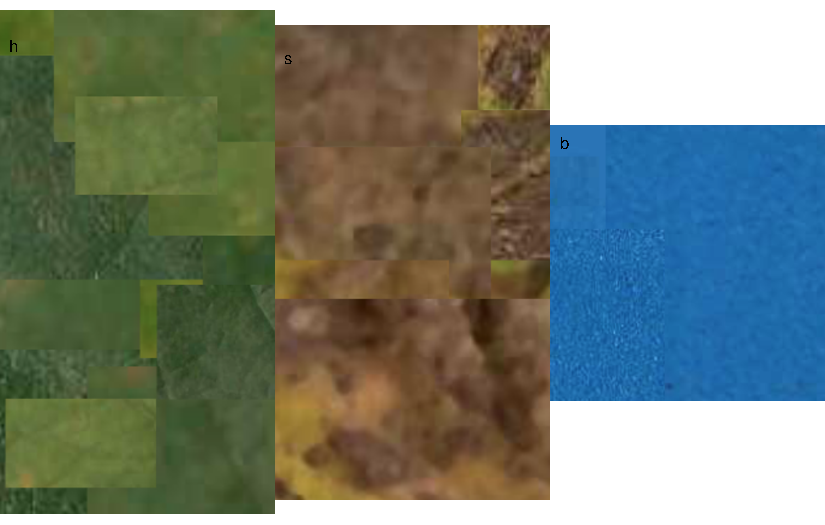
\includegraphics{./data-actual-severity_files/figure-pdf/fig-palettes-1.pdf}

}

\caption{\label{fig-palettes}Image palettes created to segment images
into background, sypomtoms and healthy area of the image}

\end{figure}

\hypertarget{measuring-severity-1}{%
\section{Measuring severity}\label{measuring-severity-1}}

\hypertarget{single-image}{%
\subsection{Single image}\label{single-image}}

To determine severity in a single image (img46.png), the image file
needs to be loaded and assigned to an object using the same
\texttt{image\_import()} function used to load the palettes. We can then
visualize the image, again using \texttt{image\_combine()}.

\begin{tcolorbox}[enhanced jigsaw, colbacktitle=quarto-callout-tip-color!10!white, toprule=.15mm, leftrule=.75mm, bottomrule=.15mm, opacitybacktitle=0.6, coltitle=black, rightrule=.15mm, left=2mm, breakable, colframe=quarto-callout-tip-color-frame, title=\textcolor{quarto-callout-tip-color}{\faLightbulb}\hspace{0.5em}{Tip}, bottomtitle=1mm, toptitle=1mm, titlerule=0mm, colback=white, arc=.35mm, opacityback=0]
The collection of images used in this chapter can be found
\href{https://github.com/emdelponte/epidemiology-R/tree/main/imgs/originals}{here}.
\end{tcolorbox}

\begin{Shaded}
\begin{Highlighting}[]
\NormalTok{img }\OtherTok{\textless{}{-}} \FunctionTok{image\_import}\NormalTok{(}\StringTok{"imgs/originals/img46.png"}\NormalTok{)}
\FunctionTok{image\_combine}\NormalTok{(img)}
\end{Highlighting}
\end{Shaded}

\begin{figure}[H]

{\centering 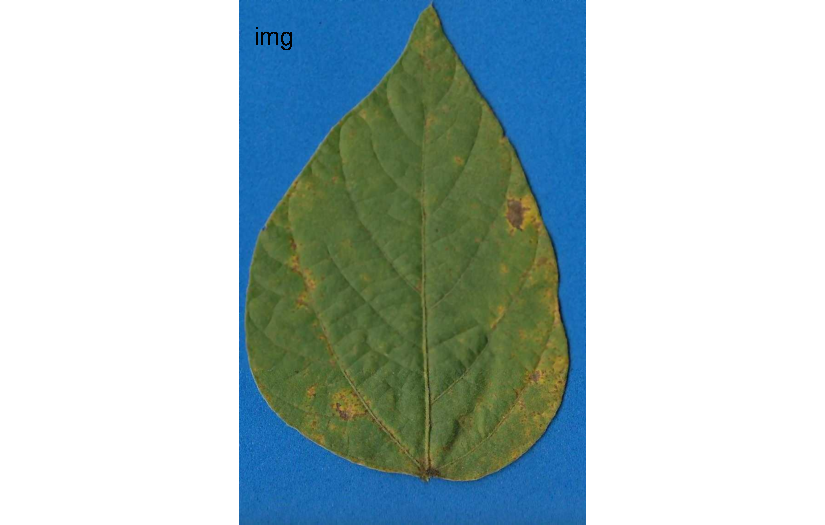
\includegraphics{./data-actual-severity_files/figure-pdf/fig-img-1.pdf}

}

\caption{\label{fig-img}Imported image for further analysis}

\end{figure}

Now the fun begins with the \texttt{measure\_disease()} function to
determine severity. Four arguments are needed when using the reference
image palettes, the one representing the target image and each of the
three images of the color palettes. As the author of the package says
``pliman will take care of all details!''. The severity is the value
shown under symptomatic in the output.

\begin{Shaded}
\begin{Highlighting}[]
\FunctionTok{set.seed}\NormalTok{(}\DecValTok{123}\NormalTok{)}
\FunctionTok{measure\_disease}\NormalTok{(}
  \AttributeTok{img =}\NormalTok{ img,}
  \AttributeTok{img\_healthy =}\NormalTok{ h,}
  \AttributeTok{img\_symptoms =}\NormalTok{ s,}
  \AttributeTok{img\_background =}\NormalTok{ b,}
  \AttributeTok{show\_image =} \ConstantTok{TRUE}
\NormalTok{)}
\end{Highlighting}
\end{Shaded}

\begin{figure}[H]

{\centering 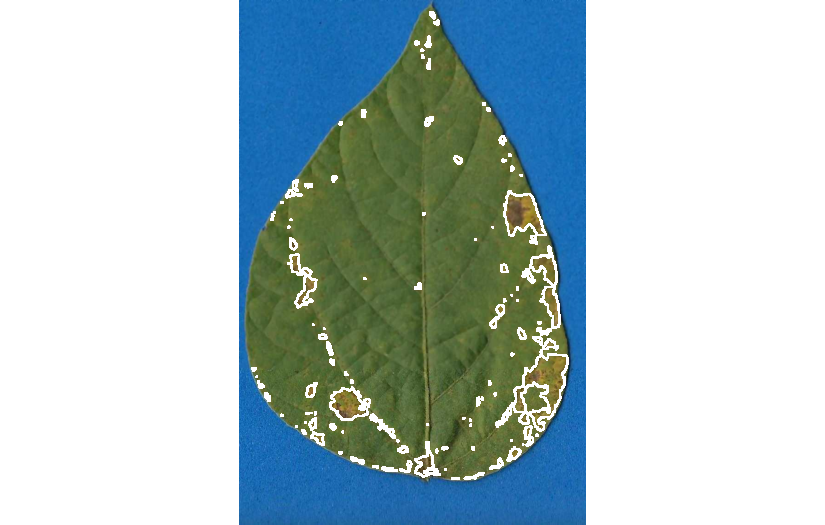
\includegraphics{./data-actual-severity_files/figure-pdf/unnamed-chunk-6-1.pdf}

}

\end{figure}

\begin{verbatim}
$severity
   healthy symptomatic
1 92.68302    7.316983

$shape
NULL

$statistics
NULL

attr(,"class")
[1] "plm_disease"
\end{verbatim}

\hypertarget{multiple-images}{%
\subsection{Multiple images}\label{multiple-images}}

Measuring severity in single images is fun, but usually we don't have a
single image to process but several. It would take a longer time to
process each one using the above procedure, thus becoming tedious.

To automate the process, \emph{pliman} offers a batch processing
approach. For such, instead of using \texttt{img} argument, one can use
\texttt{pattern} and define the prefix of names of the images. In
addition, we also need to define the folder where the original files are
located.

If the users wants to save the processed masks, the \texttt{save\_image}
argument needs to be set to TRUE and the directory where the images will
be saved also should be informed. Check below how to process 10 images
of soybean rust symptoms. The outcome is a \texttt{list} object with the
measures of the percent healthy and percent symptomatic area for each
leaf in the \texttt{severity} object.

\begin{Shaded}
\begin{Highlighting}[]
\NormalTok{pliman }\OtherTok{\textless{}{-}} \FunctionTok{measure\_disease}\NormalTok{(}
  \AttributeTok{pattern =} \StringTok{"img"}\NormalTok{,}
  \AttributeTok{dir\_original =} \StringTok{"imgs/originals"}\NormalTok{ ,}
  \AttributeTok{dir\_processed =} \StringTok{"imgs/processed"}\NormalTok{,}
  \AttributeTok{save\_image =} \ConstantTok{TRUE}\NormalTok{,}
  \AttributeTok{img\_healthy =}\NormalTok{ h,}
  \AttributeTok{img\_symptoms =}\NormalTok{ s,}
  \AttributeTok{img\_background =}\NormalTok{ b,}
  \AttributeTok{show\_image =} \ConstantTok{FALSE}
\NormalTok{)}
\end{Highlighting}
\end{Shaded}

\begin{verbatim}
Processing image img11 |====                                     | 10% 00:00:00 
\end{verbatim}

\begin{verbatim}
Processing image img35 |========                                 | 20% 00:00:02 
\end{verbatim}

\begin{verbatim}
Processing image img37 |============                             | 30% 00:00:03 
\end{verbatim}

\begin{verbatim}
Processing image img38 |================                         | 40% 00:00:03 
\end{verbatim}

\begin{verbatim}
Processing image img46 |====================                     | 50% 00:00:04 
\end{verbatim}

\begin{verbatim}
Processing image img5 |=========================                 | 60% 00:00:05 
\end{verbatim}

\begin{verbatim}
Processing image img63 |=============================            | 70% 00:00:07 
\end{verbatim}

\begin{verbatim}
Processing image img67 |=================================        | 80% 00:00:09 
\end{verbatim}

\begin{verbatim}
Processing image img70 |=====================================    | 90% 00:00:11 
\end{verbatim}

\begin{verbatim}
Processing image img75 |=========================================| 100% 00:00:12 
\end{verbatim}

\begin{Shaded}
\begin{Highlighting}[]
\NormalTok{severity }\OtherTok{\textless{}{-}}\NormalTok{ pliman}\SpecialCharTok{$}\NormalTok{severity}
\NormalTok{severity}
\end{Highlighting}
\end{Shaded}

\begin{verbatim}
     img  healthy symptomatic
1  img11 70.80072  29.1992835
2  img35 46.96430  53.0357002
3  img37 60.49390  39.5060986
4  img38 79.14737  20.8526306
5  img46 93.15143   6.8485680
6   img5 20.53977  79.4602312
7  img63 97.15698   2.8430190
8  img67 99.83723   0.1627709
9  img70 35.58683  64.4131683
10 img75 93.04517   6.9548329
\end{verbatim}

With the argument \texttt{save\_image} set to TRUE, the images are all
saved in the folder with the standard prefix ``proc.''

\begin{figure}

{\centering 

\href{fig_folder}{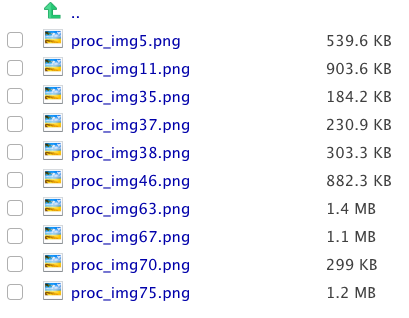
\includegraphics{./imgs/pliman2.png}}

}

\caption{Images created by pliman and exported to a specific folder}

\end{figure}

Let's have a look at one of the processed images.

\begin{figure}

{\centering 

\href{fig_proc1}{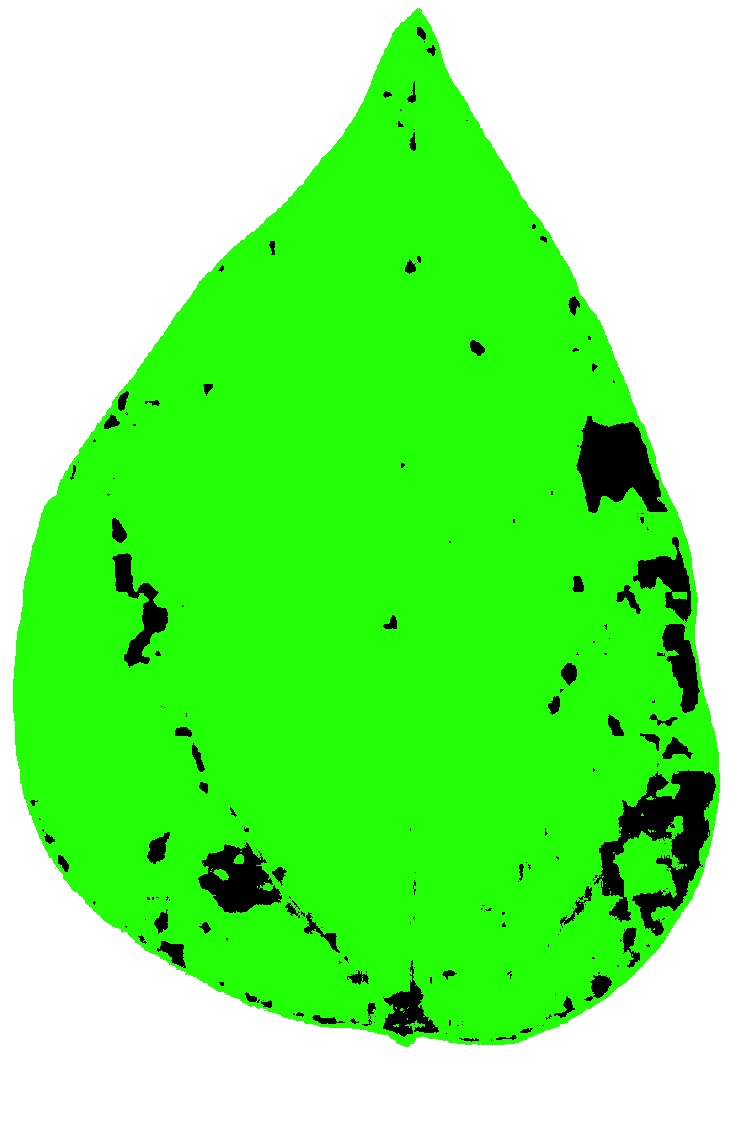
\includegraphics[width=4.70833in,height=\textheight]{./imgs/processed/proc_img46.jpg}}

}

\caption{Figure created by pliman after batch processing to segment the
images and calculate percent area covered by symptoms. The symptomatic
area is delinated in the image.}

\end{figure}

\hypertarget{how-good-are-these-measurements}{%
\section{How good are these
measurements?}\label{how-good-are-these-measurements}}

These 10 images were previously processed in QUANT software for
measuring severity which is also based on image threshold. Let's create
a tibble for the image code and respective ``actual'' severity -
assuming QUANT measures as reference.

\begin{Shaded}
\begin{Highlighting}[]
\FunctionTok{library}\NormalTok{(tidyverse)}
\NormalTok{quant }\OtherTok{\textless{}{-}} \FunctionTok{tribble}\NormalTok{(}
  \SpecialCharTok{\textasciitilde{}}\NormalTok{img, }\SpecialCharTok{\textasciitilde{}}\NormalTok{actual,}
   \StringTok{"img5"}\NormalTok{,     }\DecValTok{75}\NormalTok{,}
  \StringTok{"img11"}\NormalTok{,     }\DecValTok{24}\NormalTok{,}
  \StringTok{"img35"}\NormalTok{,     }\DecValTok{52}\NormalTok{,}
  \StringTok{"img37"}\NormalTok{,     }\DecValTok{38}\NormalTok{,}
  \StringTok{"img38"}\NormalTok{,     }\DecValTok{17}\NormalTok{,}
  \StringTok{"img46"}\NormalTok{,      }\DecValTok{7}\NormalTok{,}
  \StringTok{"img63"}\NormalTok{,    }\FloatTok{2.5}\NormalTok{,}
  \StringTok{"img67"}\NormalTok{,   }\FloatTok{0.25}\NormalTok{,}
  \StringTok{"img70"}\NormalTok{,     }\DecValTok{67}\NormalTok{,}
  \StringTok{"img75"}\NormalTok{,     }\DecValTok{10}
\NormalTok{  )}
\end{Highlighting}
\end{Shaded}

We can now combine the two dataframes and produce a scatter plot
relating the two measures.

\begin{Shaded}
\begin{Highlighting}[]
\NormalTok{dat }\OtherTok{\textless{}{-}} \FunctionTok{left\_join}\NormalTok{(severity, quant)}
\end{Highlighting}
\end{Shaded}

\begin{verbatim}
Joining, by = "img"
\end{verbatim}

\begin{Shaded}
\begin{Highlighting}[]
\NormalTok{dat }\SpecialCharTok{\%\textgreater{}\%}
  \FunctionTok{ggplot}\NormalTok{(}\FunctionTok{aes}\NormalTok{(actual, symptomatic)) }\SpecialCharTok{+}
  \FunctionTok{geom\_point}\NormalTok{(}\AttributeTok{size =} \DecValTok{5}\NormalTok{, }\AttributeTok{shape =} \DecValTok{16}\NormalTok{, }\AttributeTok{color =} \StringTok{"gray50"}\NormalTok{) }\SpecialCharTok{+}
  \FunctionTok{ylim}\NormalTok{(}\DecValTok{0}\NormalTok{, }\DecValTok{100}\NormalTok{) }\SpecialCharTok{+}
  \FunctionTok{xlim}\NormalTok{(}\DecValTok{0}\NormalTok{, }\DecValTok{100}\NormalTok{) }\SpecialCharTok{+}
  \FunctionTok{geom\_abline}\NormalTok{(}\AttributeTok{slope =} \DecValTok{1}\NormalTok{, }\AttributeTok{intercept =} \DecValTok{0}\NormalTok{) }\SpecialCharTok{+}
  \FunctionTok{theme\_light}\NormalTok{() }\SpecialCharTok{+}
  \FunctionTok{labs}\NormalTok{(}\AttributeTok{x =} \StringTok{"Quant"}\NormalTok{,}
       \AttributeTok{y =} \StringTok{"pliman"}\NormalTok{)}
\end{Highlighting}
\end{Shaded}

\begin{figure}[H]

{\centering 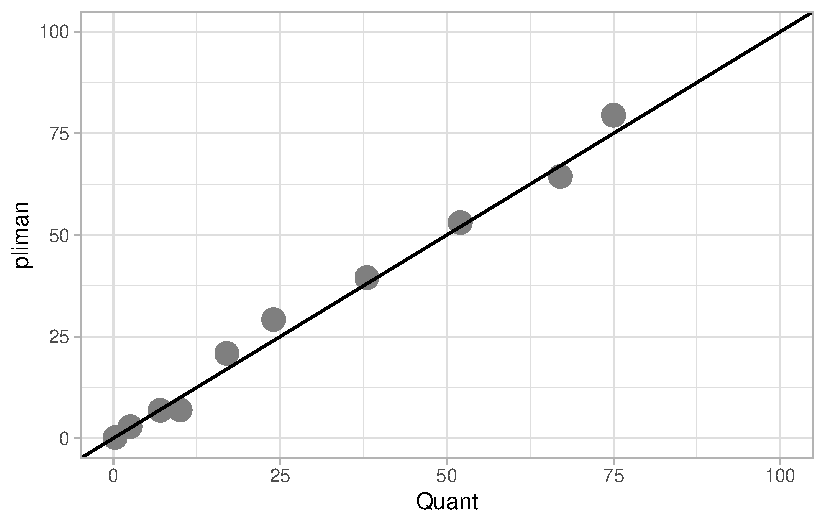
\includegraphics{./data-actual-severity_files/figure-pdf/fig-scatter-1.pdf}

}

\caption{\label{fig-scatter}Scatter plot for the relationship between
severity values measured by pliman and Quant software}

\end{figure}

The concordance correlation coefficient is a test for agreement between
two observers or two methods (see previous chapter). It is an indication
of how accurate the \emph{pliman} measures are compared with a standard.
The coefficient is greater than 0.99 (1.0 is perfect concordance),
suggesting an excellent agreement!

\begin{Shaded}
\begin{Highlighting}[]
\FunctionTok{library}\NormalTok{(epiR)}
\NormalTok{ccc }\OtherTok{\textless{}{-}} \FunctionTok{epi.ccc}\NormalTok{(dat}\SpecialCharTok{$}\NormalTok{actual, dat}\SpecialCharTok{$}\NormalTok{symptomatic)}
\NormalTok{ccc}\SpecialCharTok{$}\NormalTok{rho.c}
\end{Highlighting}
\end{Shaded}

\begin{verbatim}
        est     lower     upper
1 0.9940941 0.9774812 0.9984606
\end{verbatim}

In conclusion, the most critical step, as mentioned, is the definition
of the reference image palettes. A few preliminary runs may be needed
for a few images to check whether the segmentation is being performed
correctly, based on visual judgement. This is no different than any
other color-threshold based methods when the choices made by the user
affect the final result and contribute to variation among assessors. The
cons are the same encountered in the direct competitors, which is the
necessity to have images obtained at uniform and controlled conditions,
especially a contrasting background.

\part{Temporal analysis}

\hypertarget{disease-progress-curves}{%
\chapter{Disease progress curves}\label{disease-progress-curves}}

\begin{tcolorbox}[enhanced jigsaw, rightrule=.15mm, left=2mm, breakable, colframe=quarto-callout-note-color-frame, toprule=.15mm, leftrule=.75mm, bottomrule=.15mm, colback=white, arc=.35mm, opacityback=0]
\begin{minipage}[t]{5.5mm}
\textcolor{quarto-callout-note-color}{\faInfo}
\end{minipage}%
\begin{minipage}[t]{\textwidth - 5.5mm}
This is a work in progress that is currently undergoing heavy technical
editing and copy-editing\end{minipage}%
\end{tcolorbox}

A key understanding of the epidemics relates to the knowledge of rates
and patterns. Epidemics can be viewed as dynamic systems that change
their state as time goes. The first and simplest way to characterize
such changes in time is to produce a graphical plot called disease
progress curve (DPC). This curve can be obtained as long as the
intensity of the disease (\emph{y}) in the host population is assessed
sequentially in time (\emph{t}).

A DPC summarizes the interaction of the three main components of the
disease triangle occurring during the epidemic. The curves can vary
greatly in shape according to variations in each of the components, in
particular due to management practices that alter the course of the
epidemics and for which the goal is to stop disease increase. We can
create a dataframe in R for a single DPC and make a plot using ggplot.
By convention we use \texttt{t} for time and \texttt{y} for disease
intensity, expressed in percentage (0 to 100\%).

Firstly, let's load the essential R packages and set up the environment.

\begin{Shaded}
\begin{Highlighting}[]
\FunctionTok{library}\NormalTok{(tidyverse) }\CommentTok{\# essential packages }
\FunctionTok{library}\NormalTok{(cowplot) }\CommentTok{\# for themes }
\FunctionTok{theme\_set}\NormalTok{(}\FunctionTok{theme\_bw}\NormalTok{(}\AttributeTok{base\_size =} \DecValTok{16}\NormalTok{)) }\CommentTok{\# set global theme}
\end{Highlighting}
\end{Shaded}

There are several ways to create a dataframe in R. I like to use the
\texttt{tribble} function as below. The entered data will be assigned to
a dataframe called \texttt{dpc}.

\begin{Shaded}
\begin{Highlighting}[]
\NormalTok{dpc }\OtherTok{\textless{}{-}} 
  \FunctionTok{tribble}\NormalTok{(}
   \SpecialCharTok{\textasciitilde{}}\NormalTok{t,  }\SpecialCharTok{\textasciitilde{}}\NormalTok{y, }
   \DecValTok{0}\NormalTok{,  }\DecValTok{8}\NormalTok{, }
   \DecValTok{7}\NormalTok{,  }\DecValTok{13}\NormalTok{, }
  \DecValTok{14}\NormalTok{,  }\DecValTok{78}\NormalTok{, }
  \DecValTok{21}\NormalTok{,  }\DecValTok{92}\NormalTok{, }
  \DecValTok{28}\NormalTok{,  }\DecValTok{99}\NormalTok{, }
  \DecValTok{35}\NormalTok{, }\FloatTok{99.5}\NormalTok{, }
  \DecValTok{42}\NormalTok{, }\FloatTok{99.9}\NormalTok{, }
\NormalTok{  )}
\end{Highlighting}
\end{Shaded}

Now the plot

\begin{Shaded}
\begin{Highlighting}[]
\NormalTok{dpc }\SpecialCharTok{|\textgreater{}}
  \FunctionTok{ggplot}\NormalTok{(}\FunctionTok{aes}\NormalTok{(t, y)) }\SpecialCharTok{+}
  \FunctionTok{geom\_line}\NormalTok{(}\AttributeTok{size =} \DecValTok{1}\NormalTok{)}\SpecialCharTok{+}
  \FunctionTok{geom\_point}\NormalTok{(}\AttributeTok{size =} \DecValTok{4}\NormalTok{, }\AttributeTok{shape =} \DecValTok{16}\NormalTok{)}\SpecialCharTok{+}
  \FunctionTok{labs}\NormalTok{(}\AttributeTok{x =} \StringTok{"Assessment time (days)"}\NormalTok{,}
       \AttributeTok{y =} \StringTok{"Disease intensity (\%)"}\NormalTok{)}
\end{Highlighting}
\end{Shaded}

\begin{figure}[H]

{\centering 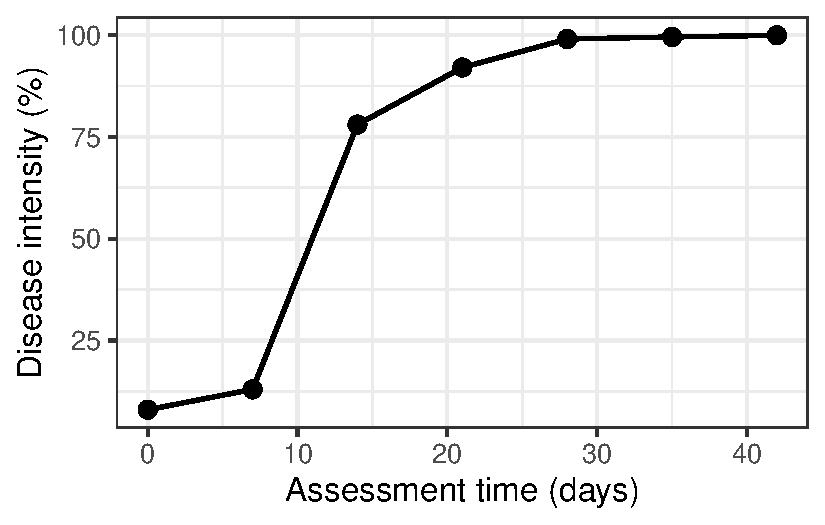
\includegraphics{./temporal-dpc_files/figure-pdf/unnamed-chunk-6-1.pdf}

}

\end{figure}

\hypertarget{curve-descriptors-audpc}{%
\section{Curve descriptors: AUDPC}\label{curve-descriptors-audpc}}

The depiction and analysis of disease progress curves can provide useful
information for gaining understanding of the underlying epidemic
process. The curves are extensively used to evaluate how disease control
measures affect epidemics. When characterizing DPCs, a researcher may be
interested in describing and comparing epidemics that result from
different treatments, or simply in their variations as affected by
changes in environment, host or pathogen.

The precision and complexity of the analysis of progress curve data
depends on the objective of the study. In general, the goal is to
synthesize similarities and different among epidemics based on common
descriptors of the disease progress curves. For example, the simple
appraisal of the disease intensity at any time during the course of the
epidemic should be sufficient for certain situations. Furthermore, a few
descriptors can be extracted including the epidemic duration, the
initial and maximum disease, and the area under the disease progress
curve (AUDPC).

The AUDPC summarizes the ``total measure of disease stress'' and is
largely used to compare epidemics (Jeger and Viljanen-Rollinson 2001).
The most common approach to calculate AUDPC is the trapezoidal method,
which splits the disease progress curves into a series of rectangles,
calculating the area of each of them and then summing the areas. Let's
extend the plot code to show those rectangles using the
\texttt{annotate} function.

\begin{Shaded}
\begin{Highlighting}[]
\FunctionTok{library}\NormalTok{(ggthemes)}
\NormalTok{dpc1 }\OtherTok{\textless{}{-}}\NormalTok{ dpc }\SpecialCharTok{|\textgreater{}}
  \FunctionTok{ggplot}\NormalTok{(}\FunctionTok{aes}\NormalTok{(t, y)) }\SpecialCharTok{+}
  \FunctionTok{labs}\NormalTok{(}\AttributeTok{x =} \StringTok{"Assessment time (days)"}\NormalTok{,}
       \AttributeTok{y =} \StringTok{"Disease intensity (\%)"}\NormalTok{)}\SpecialCharTok{+}
    \FunctionTok{geom\_area}\NormalTok{(}\AttributeTok{fill =} \StringTok{"darkorange"}\NormalTok{)}\SpecialCharTok{+}
    \FunctionTok{geom\_line}\NormalTok{(}\AttributeTok{size =} \DecValTok{1}\NormalTok{)}\SpecialCharTok{+}
  \FunctionTok{geom\_point}\NormalTok{(}\AttributeTok{size =} \DecValTok{3}\NormalTok{, }\AttributeTok{shape =} \DecValTok{16}\NormalTok{)}\SpecialCharTok{+}
  \FunctionTok{scale\_x\_continuous}\NormalTok{(}\AttributeTok{breaks =} \FunctionTok{c}\NormalTok{(}\DecValTok{0}\NormalTok{, }\DecValTok{7}\NormalTok{, }\DecValTok{14}\NormalTok{, }\DecValTok{21}\NormalTok{, }\DecValTok{28}\NormalTok{, }\DecValTok{35}\NormalTok{, }\DecValTok{42}\NormalTok{))}

\NormalTok{dpc1}
\end{Highlighting}
\end{Shaded}

\begin{figure}[H]

{\centering 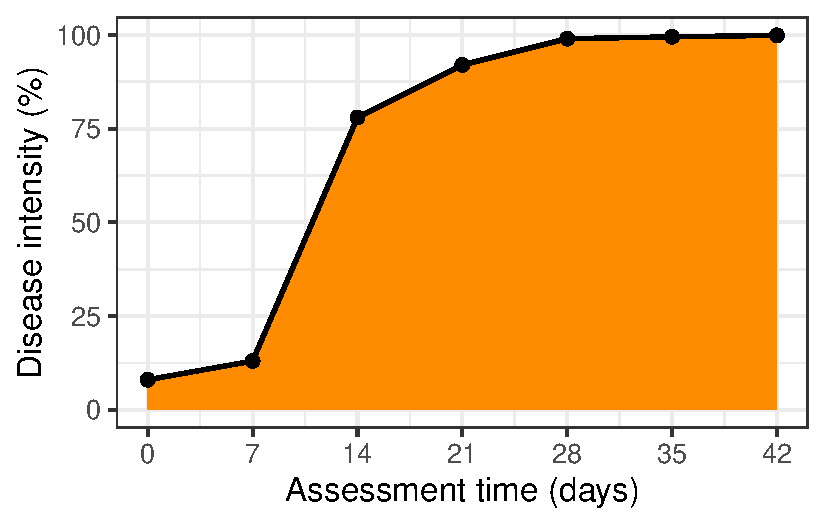
\includegraphics{./temporal-dpc_files/figure-pdf/unnamed-chunk-8-1.pdf}

}

\end{figure}

\begin{Shaded}
\begin{Highlighting}[]
\NormalTok{dpc2 }\OtherTok{\textless{}{-}}\NormalTok{ dpc }\SpecialCharTok{|\textgreater{}}
  \FunctionTok{ggplot}\NormalTok{(}\FunctionTok{aes}\NormalTok{(t, y)) }\SpecialCharTok{+}
  \FunctionTok{labs}\NormalTok{(}\AttributeTok{x =} \StringTok{"Assessment time (days)"}\NormalTok{,}
       \AttributeTok{y =} \StringTok{"Disease intensity (\%)"}\NormalTok{)}\SpecialCharTok{+}
  \FunctionTok{annotate}\NormalTok{(}\StringTok{"rect"}\NormalTok{, }\AttributeTok{xmin =}\NormalTok{ dpc}\SpecialCharTok{$}\NormalTok{t[}\DecValTok{1}\NormalTok{], }\AttributeTok{xmax =}\NormalTok{ dpc}\SpecialCharTok{$}\NormalTok{t[}\DecValTok{2}\NormalTok{], }
           \AttributeTok{ymin =} \DecValTok{0}\NormalTok{, }\AttributeTok{ymax =}\NormalTok{ (dpc}\SpecialCharTok{$}\NormalTok{y[}\DecValTok{1}\NormalTok{]}\SpecialCharTok{+}\NormalTok{ dpc}\SpecialCharTok{$}\NormalTok{y[}\DecValTok{2}\NormalTok{])}\SpecialCharTok{/}\DecValTok{2}\NormalTok{, }
           \AttributeTok{color =} \StringTok{"darkgreen"}\NormalTok{, }\AttributeTok{fill =} \StringTok{"darkorange"}\NormalTok{)}\SpecialCharTok{+}
   \FunctionTok{annotate}\NormalTok{(}\StringTok{"rect"}\NormalTok{, }\AttributeTok{xmin =}\NormalTok{ dpc}\SpecialCharTok{$}\NormalTok{t[}\DecValTok{2}\NormalTok{], }\AttributeTok{xmax =}\NormalTok{ dpc}\SpecialCharTok{$}\NormalTok{t[}\DecValTok{3}\NormalTok{], }
            \AttributeTok{ymin =} \DecValTok{0}\NormalTok{, }\AttributeTok{ymax =}\NormalTok{ (dpc}\SpecialCharTok{$}\NormalTok{y[}\DecValTok{2}\NormalTok{]}\SpecialCharTok{+}\NormalTok{ dpc}\SpecialCharTok{$}\NormalTok{y[}\DecValTok{3}\NormalTok{])}\SpecialCharTok{/}\DecValTok{2}\NormalTok{, }
            \AttributeTok{color =} \StringTok{"darkgreen"}\NormalTok{, }\AttributeTok{fill =} \StringTok{"darkorange"}\NormalTok{)}\SpecialCharTok{+}
   \FunctionTok{annotate}\NormalTok{(}\StringTok{"rect"}\NormalTok{, }\AttributeTok{xmin =}\NormalTok{ dpc}\SpecialCharTok{$}\NormalTok{t[}\DecValTok{3}\NormalTok{], }\AttributeTok{xmax =}\NormalTok{ dpc}\SpecialCharTok{$}\NormalTok{t[}\DecValTok{4}\NormalTok{], }
            \AttributeTok{ymin =} \DecValTok{0}\NormalTok{, }\AttributeTok{ymax =}\NormalTok{ (dpc}\SpecialCharTok{$}\NormalTok{y[}\DecValTok{3}\NormalTok{]}\SpecialCharTok{+}\NormalTok{ dpc}\SpecialCharTok{$}\NormalTok{y[}\DecValTok{4}\NormalTok{])}\SpecialCharTok{/}\DecValTok{2}\NormalTok{,}
            \AttributeTok{color =} \StringTok{"darkgreen"}\NormalTok{,, }\AttributeTok{fill =} \StringTok{"darkorange"}\NormalTok{)}\SpecialCharTok{+}
   \FunctionTok{annotate}\NormalTok{(}\StringTok{"rect"}\NormalTok{, }\AttributeTok{xmin =}\NormalTok{ dpc}\SpecialCharTok{$}\NormalTok{t[}\DecValTok{4}\NormalTok{], }\AttributeTok{xmax =}\NormalTok{ dpc}\SpecialCharTok{$}\NormalTok{t[}\DecValTok{5}\NormalTok{], }
            \AttributeTok{ymin =} \DecValTok{0}\NormalTok{, }\AttributeTok{ymax =}\NormalTok{ (dpc}\SpecialCharTok{$}\NormalTok{y[}\DecValTok{4}\NormalTok{]}\SpecialCharTok{+}\NormalTok{ dpc}\SpecialCharTok{$}\NormalTok{y[}\DecValTok{5}\NormalTok{])}\SpecialCharTok{/}\DecValTok{2}\NormalTok{, }
            \AttributeTok{color =} \StringTok{"darkgreen"}\NormalTok{, }\AttributeTok{fill =} \StringTok{"darkorange"}\NormalTok{)}\SpecialCharTok{+}
   \FunctionTok{annotate}\NormalTok{(}\StringTok{"rect"}\NormalTok{, }\AttributeTok{xmin =}\NormalTok{ dpc}\SpecialCharTok{$}\NormalTok{t[}\DecValTok{5}\NormalTok{], }\AttributeTok{xmax =}\NormalTok{ dpc}\SpecialCharTok{$}\NormalTok{t[}\DecValTok{6}\NormalTok{], }
            \AttributeTok{ymin =} \DecValTok{0}\NormalTok{, }\AttributeTok{ymax =}\NormalTok{ (dpc}\SpecialCharTok{$}\NormalTok{y[}\DecValTok{5}\NormalTok{]}\SpecialCharTok{+}\NormalTok{ dpc}\SpecialCharTok{$}\NormalTok{y[}\DecValTok{6}\NormalTok{])}\SpecialCharTok{/}\DecValTok{2}\NormalTok{, }
            \AttributeTok{color =} \StringTok{"darkgreen"}\NormalTok{,}\AttributeTok{fill =} \StringTok{"darkorange"}\NormalTok{)}\SpecialCharTok{+}
   \FunctionTok{annotate}\NormalTok{(}\StringTok{"rect"}\NormalTok{, }\AttributeTok{xmin =}\NormalTok{ dpc}\SpecialCharTok{$}\NormalTok{t[}\DecValTok{6}\NormalTok{], }\AttributeTok{xmax =}\NormalTok{ dpc}\SpecialCharTok{$}\NormalTok{t[}\DecValTok{7}\NormalTok{], }
            \AttributeTok{ymin =} \DecValTok{0}\NormalTok{, }\AttributeTok{ymax =}\NormalTok{ (dpc}\SpecialCharTok{$}\NormalTok{y[}\DecValTok{6}\NormalTok{]}\SpecialCharTok{+}\NormalTok{ dpc}\SpecialCharTok{$}\NormalTok{y[}\DecValTok{7}\NormalTok{])}\SpecialCharTok{/}\DecValTok{2}\NormalTok{, }
            \AttributeTok{color =} \StringTok{"darkgreen"}\NormalTok{, }\AttributeTok{fill =} \StringTok{"darkorange"}\NormalTok{)}\SpecialCharTok{+}
  \FunctionTok{geom\_line}\NormalTok{(}\AttributeTok{size =} \DecValTok{1}\NormalTok{)}\SpecialCharTok{+}
  \FunctionTok{geom\_point}\NormalTok{(}\AttributeTok{size =} \DecValTok{3}\NormalTok{, }\AttributeTok{shape =} \DecValTok{16}\NormalTok{)}\SpecialCharTok{+}
  \FunctionTok{annotate}\NormalTok{(}\AttributeTok{geom =} \StringTok{"text"}\NormalTok{, }\AttributeTok{x =} \FloatTok{26.5}\NormalTok{, }\AttributeTok{y =} \DecValTok{50}\NormalTok{,}
           \AttributeTok{label =} \StringTok{"AUDPC = 3048.5"}\NormalTok{, }\AttributeTok{size =} \DecValTok{6}\NormalTok{)}\SpecialCharTok{+}
  \FunctionTok{scale\_x\_continuous}\NormalTok{(}\AttributeTok{breaks =} \FunctionTok{c}\NormalTok{(}\DecValTok{0}\NormalTok{, }\DecValTok{7}\NormalTok{, }\DecValTok{14}\NormalTok{, }\DecValTok{21}\NormalTok{, }\DecValTok{28}\NormalTok{, }\DecValTok{35}\NormalTok{, }\DecValTok{42}\NormalTok{))}
\NormalTok{dpc2}
\end{Highlighting}
\end{Shaded}

\begin{figure}[H]

{\centering 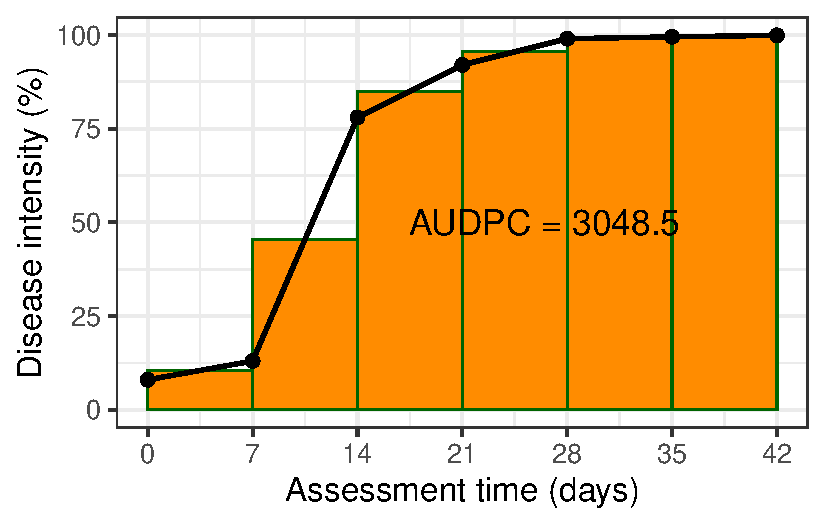
\includegraphics{./temporal-dpc_files/figure-pdf/unnamed-chunk-10-1.pdf}

}

\end{figure}

In R, we can obtain the AUDPC for the DPC we created earlier using the
\texttt{AUDPC} function offered by the \emph{epifitter} package. Because
we are using the percent data, we need to set the argument
\texttt{y\_proportion\ =\ FALSE}. The function returns the absolute
AUDPC. If one is interested in relative AUDPC, the argument
\texttt{type} should be set to \texttt{"relative"}. There is also the
alternative to AUDPC, the area under the disease progress stairs (AUDPS)
(Simko and Piepho 2012).

\begin{Shaded}
\begin{Highlighting}[]
\FunctionTok{library}\NormalTok{(epifitter)}
\FunctionTok{AUDPC}\NormalTok{(dpc}\SpecialCharTok{$}\NormalTok{t, dpc}\SpecialCharTok{$}\NormalTok{y, }
      \AttributeTok{y\_proportion =} \ConstantTok{FALSE}\NormalTok{)}
\end{Highlighting}
\end{Shaded}

\begin{verbatim}
[1] 3048.15
\end{verbatim}

\begin{Shaded}
\begin{Highlighting}[]
\CommentTok{\# The relative AUDPC }
\FunctionTok{AUDPC}\NormalTok{(dpc}\SpecialCharTok{$}\NormalTok{t, dpc}\SpecialCharTok{$}\NormalTok{y, }
      \AttributeTok{y\_proportion =} \ConstantTok{FALSE}\NormalTok{, }
      \AttributeTok{type =} \StringTok{"relative"}\NormalTok{)}
\end{Highlighting}
\end{Shaded}

\begin{verbatim}
[1] 0.72575
\end{verbatim}

\begin{Shaded}
\begin{Highlighting}[]
\CommentTok{\# To calculate AUDPS, the alternative to AUDPC}
\FunctionTok{AUDPS}\NormalTok{(dpc}\SpecialCharTok{$}\NormalTok{t, dpc}\SpecialCharTok{$}\NormalTok{y, }
      \AttributeTok{y\_proportion =} \ConstantTok{FALSE}\NormalTok{)}
\end{Highlighting}
\end{Shaded}

\begin{verbatim}
[1] 3425.8
\end{verbatim}

\hypertarget{population-models}{%
\chapter{Population models}\label{population-models}}

\begin{tcolorbox}[enhanced jigsaw, rightrule=.15mm, left=2mm, breakable, colframe=quarto-callout-note-color-frame, toprule=.15mm, leftrule=.75mm, bottomrule=.15mm, colback=white, arc=.35mm, opacityback=0]
\begin{minipage}[t]{5.5mm}
\textcolor{quarto-callout-note-color}{\faInfo}
\end{minipage}%
\begin{minipage}[t]{\textwidth - 5.5mm}
This is a work in progress that is currently undergoing heavy technical
editing and copy-editing\end{minipage}%
\end{tcolorbox}

Mathematical models can be fitted to the DPC data to express epidemic
progress in terms of rates and absolute/relative quantities. The latter
can be accomplished using population dynamics (or growth-curve) models
for which the estimated parameters are usually meaningful biologically
and appropriately describe epidemics that do not decrease in disease
intensity. By fitting an appropriate model to the progress curve data,
another set of parameters is available to the researcher when attempting
to represent, understand or compare epidemics.

The family of models that describe the growth of epidemics, hence
population dynamics model, are known as deterministic models of
continuous time (Madden et al. 2017b). These models are usually fitted
to DPC data to obtain two or more biologically meaningful parameters.
Here, these models and their formulations are shown using R scripts to
simulate the theoretical curves for each model.

\hypertarget{non-flexible-models}{%
\subsection{Non-flexible models}\label{non-flexible-models}}

These population dynamics models require at least two parameters, hence
they are known as non-flexible, as opposed to the flexible ones for
which there are at least one additional (third) parameter.

Following the convention proposed by (Madden et al. 2017b) in their book
``The study of plant disease epidemics'':

\begin{itemize}
\item
  time is represented by \(t\)
\item
  disease intensity by \(y\)
\item
  the rate of change in \(y\) between two time units is represented by
  \(\frac{dy}{dt}\)
\end{itemize}

Now we can proceed and learn which non-flexible models exist and for
which situation they are more appropriate.

\hypertarget{exponential}{%
\subsubsection{Exponential}\label{exponential}}

The differential equation for the exponential model is given by

\(\frac{dy}{dt} = r_E.y\),

where \(r_E\) is the apparent infection rate (subscript E for this
model) (sensu Vanderplank) and \(y\) is the disease intensity.
Biologically, this formulation suggests that diseased plants, or \(y\),
and \(r_E\) at each time contribute to disease increase. The value of
\(\frac{dy}{dt}\) is minimal when \(y = 0\) and increases exponentially
with the increase in \(y\).

The integral for the exponential model is given by

\(y = y_0 e^{r_Et}\),

where \(y0\) is and \(r\) are obtained via estimation. Let's simulate
two curves by varying \(r\) while fixing \(y0\) and varying the latter
while fixing \(r_E\). We produce the two plots in \emph{ggplot} and add
the predicted curve using the `stat\_function`. But first, we need to
define values for the two model parameters. Further modifications to
these values will be handled directly in the simulation (e.g.~doubling
infection rate, reducing initial inoculum by half, etc.).

\begin{Shaded}
\begin{Highlighting}[]
\FunctionTok{library}\NormalTok{(tidyverse) }\CommentTok{\# essential packages }
\FunctionTok{library}\NormalTok{(cowplot) }\CommentTok{\# for themes }
\FunctionTok{theme\_set}\NormalTok{(}\FunctionTok{theme\_bw}\NormalTok{(}\AttributeTok{base\_size =} \DecValTok{16}\NormalTok{)) }\CommentTok{\# set global theme}
\end{Highlighting}
\end{Shaded}

\begin{Shaded}
\begin{Highlighting}[]
\NormalTok{y0 }\OtherTok{\textless{}{-}} \FloatTok{0.001} 
\NormalTok{r }\OtherTok{\textless{}{-}} \FloatTok{0.06} 
\NormalTok{tmax }\OtherTok{\textless{}{-}} \DecValTok{60} \CommentTok{\# maximum duration t of the epidemics}
\NormalTok{dat }\OtherTok{\textless{}{-}} \FunctionTok{data.frame}\NormalTok{(}\AttributeTok{t =} \FunctionTok{seq}\NormalTok{(}\DecValTok{1}\SpecialCharTok{:}\NormalTok{tmax), }\AttributeTok{y =} \FunctionTok{seq}\NormalTok{(}\DecValTok{0}\SpecialCharTok{:}\DecValTok{1}\NormalTok{)) }\CommentTok{\# define the axes}
\end{Highlighting}
\end{Shaded}

In the plot below, note that the infection rate in one curve was doubled
(\(r\) = 0.12)

\begin{Shaded}
\begin{Highlighting}[]
\NormalTok{dat }\SpecialCharTok{|\textgreater{}}
  \FunctionTok{ggplot}\NormalTok{(}\FunctionTok{aes}\NormalTok{(t, y)) }\SpecialCharTok{+}
  \FunctionTok{stat\_function}\NormalTok{(}\AttributeTok{fun =} \ControlFlowTok{function}\NormalTok{(t) y0 }\SpecialCharTok{*} \FunctionTok{exp}\NormalTok{(r }\SpecialCharTok{*}\NormalTok{ t), }\AttributeTok{linetype =} \DecValTok{1}\NormalTok{) }\SpecialCharTok{+}
  \FunctionTok{stat\_function}\NormalTok{(}\AttributeTok{fun =} \ControlFlowTok{function}\NormalTok{(t) y0 }\SpecialCharTok{*} \FunctionTok{exp}\NormalTok{(r }\SpecialCharTok{*} \DecValTok{2} \SpecialCharTok{*}\NormalTok{ t), }\AttributeTok{linetype =} \DecValTok{2}\NormalTok{) }\SpecialCharTok{+}
  \FunctionTok{ylim}\NormalTok{(}\DecValTok{0}\NormalTok{, }\DecValTok{1}\NormalTok{) }\SpecialCharTok{+}
  \FunctionTok{labs}\NormalTok{(}
    \AttributeTok{title =} \StringTok{"Exponential model"}\NormalTok{,}
    \AttributeTok{subtitle =} \StringTok{"2 times r (dashed) same y0"}\NormalTok{,}
    \AttributeTok{x =} \StringTok{"Time"}
\NormalTok{  )}
\end{Highlighting}
\end{Shaded}

\begin{verbatim}
Warning: Removed 5 row(s) containing missing values (geom_path).
\end{verbatim}

\begin{figure}[H]

{\centering 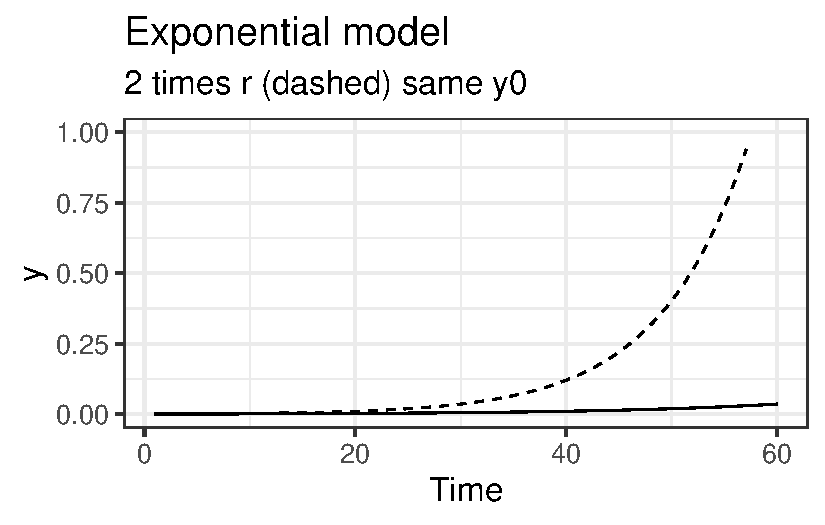
\includegraphics{./temporal-models_files/figure-pdf/unnamed-chunk-6-1.pdf}

}

\end{figure}

Now the inoculum was increased five times while using the same doubled
rate.

\begin{Shaded}
\begin{Highlighting}[]
\NormalTok{dat }\SpecialCharTok{|\textgreater{}}
  \FunctionTok{ggplot}\NormalTok{(}\FunctionTok{aes}\NormalTok{(t, y)) }\SpecialCharTok{+}
  \FunctionTok{stat\_function}\NormalTok{(}\AttributeTok{fun =} \ControlFlowTok{function}\NormalTok{(t) y0 }\SpecialCharTok{*} \FunctionTok{exp}\NormalTok{(r }\SpecialCharTok{*} \DecValTok{2} \SpecialCharTok{*}\NormalTok{ t), }\AttributeTok{linetype =} \DecValTok{1}\NormalTok{) }\SpecialCharTok{+}
  \FunctionTok{stat\_function}\NormalTok{(}\AttributeTok{fun =} \ControlFlowTok{function}\NormalTok{(t) y0 }\SpecialCharTok{*} \DecValTok{5} \SpecialCharTok{*} \FunctionTok{exp}\NormalTok{(r }\SpecialCharTok{*} \DecValTok{2} \SpecialCharTok{*}\NormalTok{ t), }\AttributeTok{linetype =} \DecValTok{2}\NormalTok{) }\SpecialCharTok{+}
  \FunctionTok{ylim}\NormalTok{(}\DecValTok{0}\NormalTok{, }\DecValTok{1}\NormalTok{) }\SpecialCharTok{+}
  \FunctionTok{labs}\NormalTok{(}\AttributeTok{title =} \StringTok{"Exponential model"}\NormalTok{, }\AttributeTok{x =} \StringTok{"Time"}\NormalTok{,}
       \AttributeTok{subtitle =} \StringTok{"5 times y0 (dashed) same r"}\NormalTok{)}
\end{Highlighting}
\end{Shaded}

\begin{verbatim}
Warning: Removed 5 row(s) containing missing values (geom_path).
\end{verbatim}

\begin{verbatim}
Warning: Removed 27 row(s) containing missing values (geom_path).
\end{verbatim}

\begin{figure}[H]

{\centering 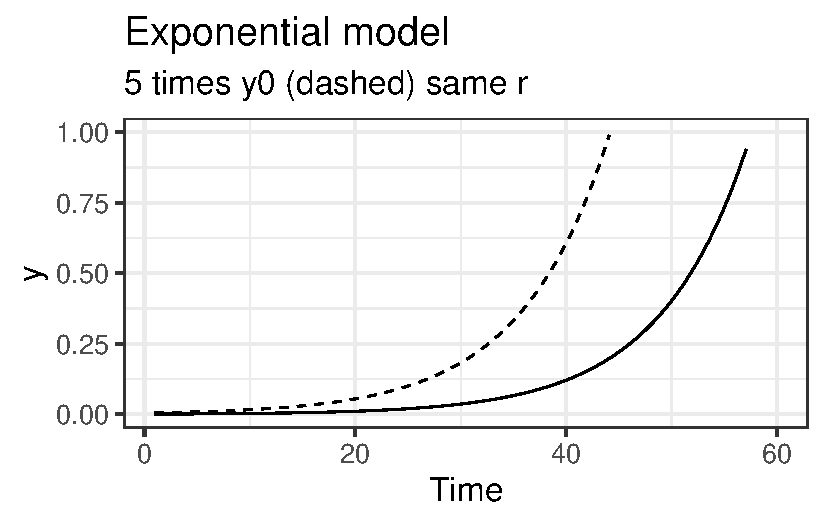
\includegraphics{./temporal-models_files/figure-pdf/unnamed-chunk-8-1.pdf}

}

\end{figure}

\hypertarget{monomolecular}{%
\subsubsection{Monomolecular}\label{monomolecular}}

The differential of the monomolecular model is given by

\(\frac{dy}{dt} = r_M (1-y)\)

where now the \(r_M\) is the rate parameter of the monomolecular model
and \((1-y)\) is the proportion of non-infected (healthy) individuals or
host tissue. Note that \(\frac{dy}{dt}\) is maximum when \(y = 0\) and
decreases when \(y\) approaches 1. Its decline is due to decrease in the
proportion of individuals or healthy sites with the increase in \(y\).
Any inoculum capable of infecting the host will more likely land on
infected individuals or sites.

The integral of the monomolecular model is given by

\(\frac{dy}{dt} = 1 - (1-y)e^{-r_Mt}\)

This model commonly describes the temporal patterns of the monocyclic
epidemics. In those, the inoculum produced during the course of the
epidemics do not contribute new infections. Therefore, different from
the exponential model, disease intensity \(y\) does not affect the
epidemics and so the absolute rate is proportional to \((1-y)\).

Let's simulate two monomolecular curve with different rate parameters
where one is one third of the other.

\begin{Shaded}
\begin{Highlighting}[]
\NormalTok{dat }\SpecialCharTok{|\textgreater{}}
  \FunctionTok{ggplot}\NormalTok{(}\FunctionTok{aes}\NormalTok{(t, y)) }\SpecialCharTok{+}
  \FunctionTok{stat\_function}\NormalTok{(}\AttributeTok{fun =} \ControlFlowTok{function}\NormalTok{(t) }\DecValTok{1} \SpecialCharTok{{-}}\NormalTok{ ((}\DecValTok{1} \SpecialCharTok{{-}}\NormalTok{ y0) }\SpecialCharTok{*} \FunctionTok{exp}\NormalTok{(}\SpecialCharTok{{-}}\NormalTok{r }\SpecialCharTok{*}\NormalTok{ t))) }\SpecialCharTok{+}
  \FunctionTok{stat\_function}\NormalTok{(}\AttributeTok{fun =} \ControlFlowTok{function}\NormalTok{(t) }\DecValTok{1} \SpecialCharTok{{-}}\NormalTok{ ((}\DecValTok{1} \SpecialCharTok{{-}}\NormalTok{ y0) }\SpecialCharTok{*} \FunctionTok{exp}\NormalTok{(}\SpecialCharTok{{-}}\NormalTok{(r }\SpecialCharTok{/} \DecValTok{3}\NormalTok{) }\SpecialCharTok{*}\NormalTok{ t))) }\SpecialCharTok{+}
  \FunctionTok{labs}\NormalTok{(}\AttributeTok{title =} \StringTok{"Monomolecular model"}\NormalTok{,}
         \AttributeTok{subtitle =} \StringTok{"Fixed y0 = 0.001"}\NormalTok{, }\AttributeTok{x =} \StringTok{"Time"}
\NormalTok{       ) }\SpecialCharTok{+}
  \FunctionTok{annotate}\NormalTok{(}\AttributeTok{geom =} \StringTok{"text"}\NormalTok{, }\AttributeTok{x =} \DecValTok{35}\NormalTok{, }\AttributeTok{y =} \FloatTok{0.77}\NormalTok{, }\AttributeTok{label =} \StringTok{"r = 0.06"}\NormalTok{) }\SpecialCharTok{+}
  \FunctionTok{annotate}\NormalTok{(}\AttributeTok{geom =} \StringTok{"text"}\NormalTok{, }\AttributeTok{x =} \DecValTok{50}\NormalTok{, }\AttributeTok{y =} \FloatTok{0.55}\NormalTok{, }\AttributeTok{label =} \StringTok{"r = 0.02"}\NormalTok{)}
\end{Highlighting}
\end{Shaded}

\begin{figure}[H]

{\centering 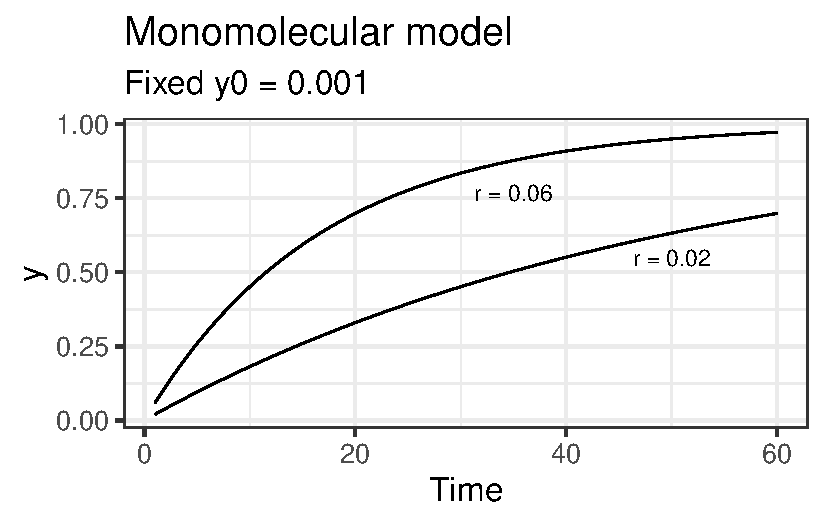
\includegraphics{./temporal-models_files/figure-pdf/unnamed-chunk-10-1.pdf}

}

\end{figure}

Now inoculum was increased 100 times with the reduced rate.

\begin{Shaded}
\begin{Highlighting}[]
\NormalTok{dat }\SpecialCharTok{|\textgreater{}}
  \FunctionTok{ggplot}\NormalTok{(}\FunctionTok{aes}\NormalTok{(t, y)) }\SpecialCharTok{+}
  \FunctionTok{stat\_function}\NormalTok{(}\AttributeTok{fun =} \ControlFlowTok{function}\NormalTok{(t) }\DecValTok{1} \SpecialCharTok{{-}}\NormalTok{ ((}\DecValTok{1} \SpecialCharTok{{-}}\NormalTok{ y0) }\SpecialCharTok{*} \FunctionTok{exp}\NormalTok{(}\SpecialCharTok{{-}}\NormalTok{r }\SpecialCharTok{/} \DecValTok{2} \SpecialCharTok{*}\NormalTok{ t))) }\SpecialCharTok{+}
  \FunctionTok{stat\_function}\NormalTok{(}\AttributeTok{fun =} \ControlFlowTok{function}\NormalTok{(t) }\DecValTok{1} \SpecialCharTok{{-}}\NormalTok{ ((}\DecValTok{1} \SpecialCharTok{{-}}\NormalTok{ (y0 }\SpecialCharTok{*} \DecValTok{100}\NormalTok{)) }\SpecialCharTok{*} \FunctionTok{exp}\NormalTok{(}\SpecialCharTok{{-}}\NormalTok{r }\SpecialCharTok{/} \DecValTok{2} \SpecialCharTok{*}\NormalTok{ t))) }\SpecialCharTok{+}
  \FunctionTok{labs}\NormalTok{(}\AttributeTok{title =} \StringTok{"Monomolecular model"}\NormalTok{, }
       \AttributeTok{subtitle =} \StringTok{"Fixed r = 0.06"}\NormalTok{, }\AttributeTok{x =} \StringTok{"Time"}\NormalTok{) }\SpecialCharTok{+}
  \FunctionTok{annotate}\NormalTok{(}\AttributeTok{geom =} \StringTok{"text"}\NormalTok{, }\AttributeTok{x =} \DecValTok{35}\NormalTok{, }\AttributeTok{y =} \FloatTok{0.77}\NormalTok{, }\AttributeTok{label =} \StringTok{"y0 = 0.01"}\NormalTok{) }\SpecialCharTok{+}
  \FunctionTok{annotate}\NormalTok{(}\AttributeTok{geom =} \StringTok{"text"}\NormalTok{, }\AttributeTok{x =} \DecValTok{45}\NormalTok{, }\AttributeTok{y =} \FloatTok{0.65}\NormalTok{, }\AttributeTok{label =} \StringTok{"y0 = 0.001"}\NormalTok{)}
\end{Highlighting}
\end{Shaded}

\begin{figure}[H]

{\centering 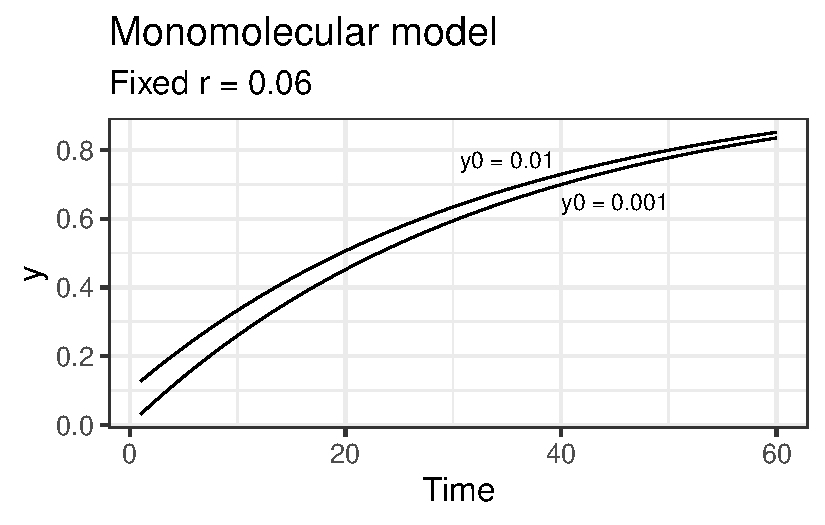
\includegraphics{./temporal-models_files/figure-pdf/unnamed-chunk-12-1.pdf}

}

\end{figure}

\hypertarget{logistic}{%
\subsubsection{Logistic}\label{logistic}}

The logistic model is a more elaborated version of the two previous
models as it incorporates the features of them both. Its differential is
given by

\(\frac{dy}{dt} = r_L. y . (1 - y)\),

where \(r_L\) is the infection rate of the logistic model, \(y\) is the
proportion of diseased individuals or host tissue and \((1-y)\) is the
proportion of non-affected individuals or host area.

Biologically, \(y\) in its differential equation implies that
\(\frac{dy}{dt}\) increases with the increase in \(y\) (as in the
exponential) because more disease means more inoculum. However,
\((1-y)\) leads to a decrease in \(\frac{dy}{dt}\) when \(y\) approaches
the maximum \(y=1\), because the proportion of healthy individuals or
host area decreases (as in the monomolecular). Therefore,
\(\frac{dy}{dt}\) is minimal at the onset of the epidemics, reaches a
maximum when \(y/2\) and declines until \(y=1\).

The integral is given by

\(y = \frac{1}{1 + (1-y_0).e^{-r.t}}\),

where \(r_L\) is the apparent infection rate of the logistic model and
\(y0\) is the disease intensity at \(t=0\). This model provides a good
fit to polycyclic epidemics.

Let's check two curves where in one the infection rate is double while
keeping the same initial inoculum.

\begin{Shaded}
\begin{Highlighting}[]
\NormalTok{dat }\SpecialCharTok{|\textgreater{}}
  \FunctionTok{ggplot}\NormalTok{(}\FunctionTok{aes}\NormalTok{(t, y)) }\SpecialCharTok{+}
  \FunctionTok{stat\_function}\NormalTok{(}
    \AttributeTok{linetype =} \DecValTok{2}\NormalTok{,}
    \AttributeTok{fun =} \ControlFlowTok{function}\NormalTok{(t) }\DecValTok{1} \SpecialCharTok{/}\NormalTok{ (}\DecValTok{1} \SpecialCharTok{+}\NormalTok{ ((}\DecValTok{1} \SpecialCharTok{{-}}\NormalTok{ y0) }\SpecialCharTok{/}\NormalTok{ y0) }\SpecialCharTok{*} \FunctionTok{exp}\NormalTok{(}\SpecialCharTok{{-}}\NormalTok{r }\SpecialCharTok{*} \DecValTok{2} \SpecialCharTok{*}\NormalTok{ t))}
\NormalTok{  ) }\SpecialCharTok{+}
  \FunctionTok{stat\_function}\NormalTok{(}\AttributeTok{fun =} \ControlFlowTok{function}\NormalTok{(t) }\DecValTok{1} \SpecialCharTok{/}\NormalTok{ (}\DecValTok{1} \SpecialCharTok{+}\NormalTok{ ((}\DecValTok{1} \SpecialCharTok{{-}}\NormalTok{ y0) }\SpecialCharTok{/}\NormalTok{ y0) }\SpecialCharTok{*} \FunctionTok{exp}\NormalTok{(}\SpecialCharTok{{-}}\NormalTok{r }\SpecialCharTok{*} \DecValTok{4} \SpecialCharTok{*}\NormalTok{ t))) }\SpecialCharTok{+}
  \FunctionTok{labs}\NormalTok{(}\AttributeTok{title =} \StringTok{"Logistic model"}\NormalTok{, }\AttributeTok{subtitle =} \StringTok{"Fixed y0 = 0.001"}\NormalTok{, }\AttributeTok{x =} \StringTok{"Time"}\NormalTok{) }\SpecialCharTok{+}
  \FunctionTok{annotate}\NormalTok{(}\AttributeTok{geom =} \StringTok{"text"}\NormalTok{, }\AttributeTok{x =} \DecValTok{41}\NormalTok{, }\AttributeTok{y =} \FloatTok{0.77}\NormalTok{, }\AttributeTok{label =} \StringTok{"r = 0.18"}\NormalTok{) }\SpecialCharTok{+}
  \FunctionTok{annotate}\NormalTok{(}\AttributeTok{geom =} \StringTok{"text"}\NormalTok{, }\AttributeTok{x =} \DecValTok{50}\NormalTok{, }\AttributeTok{y =} \FloatTok{0.10}\NormalTok{, }\AttributeTok{label =} \StringTok{"r = 0.024"}\NormalTok{)}
\end{Highlighting}
\end{Shaded}

\begin{figure}[H]

{\centering 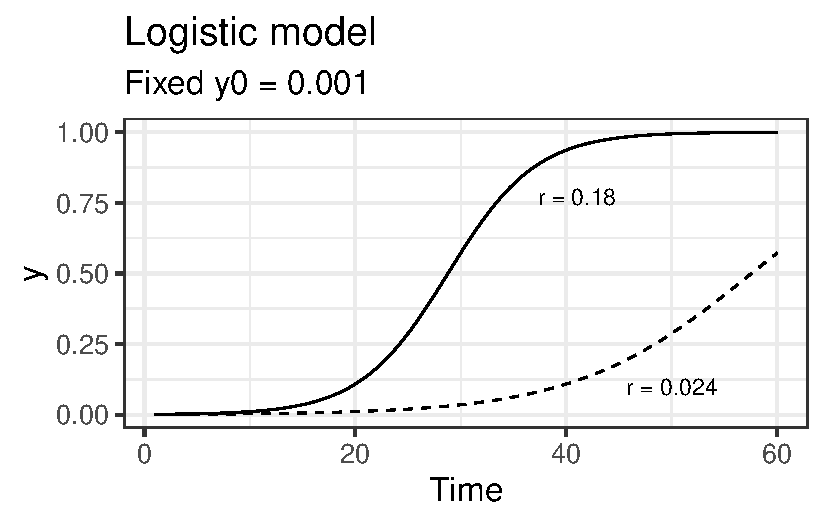
\includegraphics{./temporal-models_files/figure-pdf/unnamed-chunk-14-1.pdf}

}

\end{figure}

Now the inoculum is reduced 10 times for a same infection rate.

\begin{Shaded}
\begin{Highlighting}[]
\NormalTok{dat }\SpecialCharTok{|\textgreater{}}
  \FunctionTok{ggplot}\NormalTok{(}\FunctionTok{aes}\NormalTok{(t, y)) }\SpecialCharTok{+}
  \FunctionTok{stat\_function}\NormalTok{(}
    \AttributeTok{linetype =} \DecValTok{2}\NormalTok{,}
    \AttributeTok{fun =} \ControlFlowTok{function}\NormalTok{(t) }\DecValTok{1} \SpecialCharTok{/}\NormalTok{ (}\DecValTok{1} \SpecialCharTok{+}\NormalTok{ ((}\DecValTok{1} \SpecialCharTok{{-}}\NormalTok{ (y0 }\SpecialCharTok{/} \DecValTok{10}\NormalTok{)) }\SpecialCharTok{/}\NormalTok{ (y0 }\SpecialCharTok{/} \DecValTok{10}\NormalTok{)) }\SpecialCharTok{*} \FunctionTok{exp}\NormalTok{(}\SpecialCharTok{{-}}\NormalTok{r }\SpecialCharTok{*} \DecValTok{3} \SpecialCharTok{*}\NormalTok{ t))}
\NormalTok{  ) }\SpecialCharTok{+}
  \FunctionTok{stat\_function}\NormalTok{(}\AttributeTok{fun =} \ControlFlowTok{function}\NormalTok{(t) }\DecValTok{1} \SpecialCharTok{/}\NormalTok{ (}\DecValTok{1} \SpecialCharTok{+}\NormalTok{ ((}\DecValTok{1} \SpecialCharTok{{-}}\NormalTok{ y0) }\SpecialCharTok{/}\NormalTok{ y0) }\SpecialCharTok{*} \FunctionTok{exp}\NormalTok{(}\SpecialCharTok{{-}}\NormalTok{r }\SpecialCharTok{*} \DecValTok{3} \SpecialCharTok{*}\NormalTok{ t))) }\SpecialCharTok{+}
  \FunctionTok{labs}\NormalTok{(}\AttributeTok{title =} \StringTok{"Logistic model"}\NormalTok{, }\AttributeTok{subtitle =} \StringTok{"Fixed r = 0.24"}\NormalTok{, }\AttributeTok{x =} \StringTok{"Time"}\NormalTok{) }\SpecialCharTok{+}
  \FunctionTok{annotate}\NormalTok{(}\AttributeTok{geom =} \StringTok{"text"}\NormalTok{, }\AttributeTok{x =} \DecValTok{35}\NormalTok{, }\AttributeTok{y =} \FloatTok{0.77}\NormalTok{, }\AttributeTok{label =} \StringTok{"y0 = 0.001"}\NormalTok{) }\SpecialCharTok{+}
  \FunctionTok{annotate}\NormalTok{(}\AttributeTok{geom =} \StringTok{"text"}\NormalTok{, }\AttributeTok{x =} \DecValTok{50}\NormalTok{, }\AttributeTok{y =} \FloatTok{0.10}\NormalTok{, }\AttributeTok{label =} \StringTok{"y0 = 0.0001"}\NormalTok{)}
\end{Highlighting}
\end{Shaded}

\begin{figure}[H]

{\centering 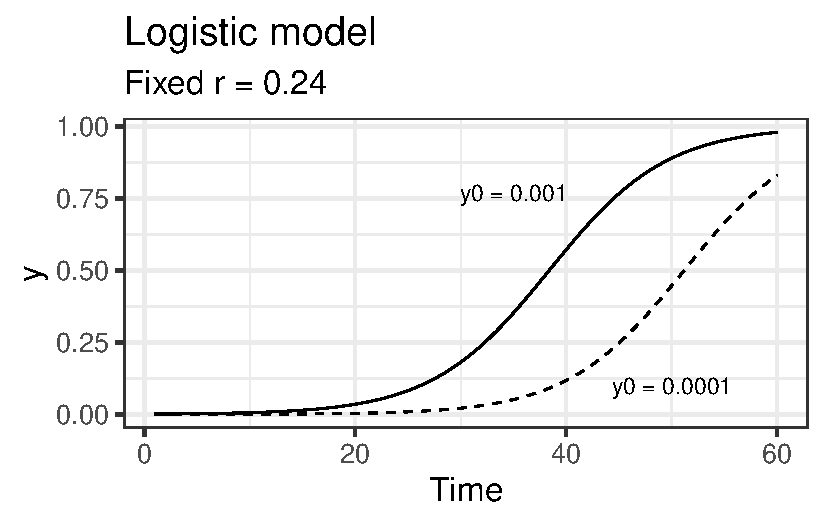
\includegraphics{./temporal-models_files/figure-pdf/unnamed-chunk-16-1.pdf}

}

\end{figure}

\hypertarget{gompertz}{%
\subsubsection{Gompertz}\label{gompertz}}

The Gompertz model is similar to the logistic and also provides a very
good fit to several polycyclic diseases. The differential equation is
given by

\(\frac{dy}{dt} = r_G.[ln(1) - ln(y)]\)

Differently from the logistic, the variable representing the
non-infected individuals or host area is \(-ln(y)\). The integral
equation is given by

\(y = e^{(ln(y0)).{e^{-r_G.t)}}}\),

where \(r_G\) is the apparent infection rate for the Gompertz models and
\(y_0\) is the disease intensity at \(t = 0\).

Let's check curves for two rates.

\begin{Shaded}
\begin{Highlighting}[]
\NormalTok{dat }\SpecialCharTok{|\textgreater{}}
  \FunctionTok{ggplot}\NormalTok{(}\FunctionTok{aes}\NormalTok{(t, y)) }\SpecialCharTok{+}
  \FunctionTok{stat\_function}\NormalTok{(}
    \AttributeTok{linetype =} \DecValTok{2}\NormalTok{,}
    \AttributeTok{fun =} \ControlFlowTok{function}\NormalTok{(t) }\FunctionTok{exp}\NormalTok{(}\FunctionTok{log}\NormalTok{(y0) }\SpecialCharTok{*} \FunctionTok{exp}\NormalTok{(}\SpecialCharTok{{-}}\NormalTok{r}\SpecialCharTok{/}\DecValTok{2} \SpecialCharTok{*}\NormalTok{ t))}
\NormalTok{  ) }\SpecialCharTok{+}
  \FunctionTok{stat\_function}\NormalTok{(}\AttributeTok{fun =} \ControlFlowTok{function}\NormalTok{(t) }\FunctionTok{exp}\NormalTok{(}\FunctionTok{log}\NormalTok{(y0) }\SpecialCharTok{*} \FunctionTok{exp}\NormalTok{(}\SpecialCharTok{{-}}\NormalTok{r}\SpecialCharTok{*}\DecValTok{2} \SpecialCharTok{*}\NormalTok{ t))) }\SpecialCharTok{+}
  \FunctionTok{labs}\NormalTok{(}\AttributeTok{title =} \StringTok{"Gompertz model"}\NormalTok{, }\AttributeTok{subtitle =} \StringTok{"Fixed y0 = 0.001"}\NormalTok{, }\AttributeTok{x =} \StringTok{"Time"}\NormalTok{) }\SpecialCharTok{+}
  \FunctionTok{annotate}\NormalTok{(}\AttributeTok{geom =} \StringTok{"text"}\NormalTok{, }\AttributeTok{x =} \DecValTok{41}\NormalTok{, }\AttributeTok{y =} \FloatTok{0.77}\NormalTok{, }\AttributeTok{label =} \StringTok{"r = 0.12"}\NormalTok{) }\SpecialCharTok{+}
  \FunctionTok{annotate}\NormalTok{(}\AttributeTok{geom =} \StringTok{"text"}\NormalTok{, }\AttributeTok{x =} \DecValTok{50}\NormalTok{, }\AttributeTok{y =} \FloatTok{0.10}\NormalTok{, }\AttributeTok{label =} \StringTok{"r = 0.03"}\NormalTok{)}
\end{Highlighting}
\end{Shaded}

\begin{figure}[H]

{\centering 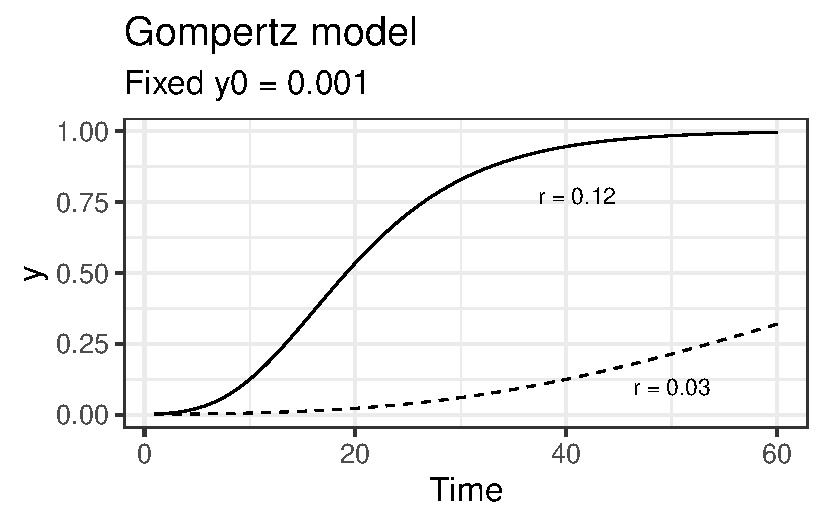
\includegraphics{./temporal-models_files/figure-pdf/unnamed-chunk-18-1.pdf}

}

\end{figure}

And those when inoculum was reduced thousand times.

\begin{Shaded}
\begin{Highlighting}[]
\NormalTok{dat }\SpecialCharTok{|\textgreater{}}
  \FunctionTok{ggplot}\NormalTok{(}\FunctionTok{aes}\NormalTok{(t, y)) }\SpecialCharTok{+}
  \FunctionTok{stat\_function}\NormalTok{(}
    \AttributeTok{linetype =} \DecValTok{2}\NormalTok{,}
    \AttributeTok{fun =} \ControlFlowTok{function}\NormalTok{(t) }\FunctionTok{exp}\NormalTok{(}\FunctionTok{log}\NormalTok{(y0) }\SpecialCharTok{*} \FunctionTok{exp}\NormalTok{(}\SpecialCharTok{{-}}\NormalTok{r}\SpecialCharTok{*}\DecValTok{2} \SpecialCharTok{*}\NormalTok{ t))}
\NormalTok{  ) }\SpecialCharTok{+}
  \FunctionTok{stat\_function}\NormalTok{(}\AttributeTok{fun =} \ControlFlowTok{function}\NormalTok{(t) }\FunctionTok{exp}\NormalTok{(}\FunctionTok{log}\NormalTok{(y0}\SpecialCharTok{/}\DecValTok{1000}\NormalTok{) }\SpecialCharTok{*} \FunctionTok{exp}\NormalTok{(}\SpecialCharTok{{-}}\NormalTok{r}\SpecialCharTok{*}\DecValTok{2} \SpecialCharTok{*}\NormalTok{ t))) }\SpecialCharTok{+}
  \FunctionTok{labs}\NormalTok{(}\AttributeTok{title =} \StringTok{"Gompertz model"}\NormalTok{, }\AttributeTok{subtitle =} \StringTok{"Fixed r = 0.12"}\NormalTok{, }\AttributeTok{x =} \StringTok{"Time"}\NormalTok{) }\SpecialCharTok{+}
  \FunctionTok{annotate}\NormalTok{(}\AttributeTok{geom =} \StringTok{"text"}\NormalTok{, }\AttributeTok{x =} \DecValTok{15}\NormalTok{, }\AttributeTok{y =} \FloatTok{0.77}\NormalTok{, }\AttributeTok{label =} \StringTok{"y0 = 0.001"}\NormalTok{) }\SpecialCharTok{+}
  \FunctionTok{annotate}\NormalTok{(}\AttributeTok{geom =} \StringTok{"text"}\NormalTok{, }\AttributeTok{x =} \DecValTok{25}\NormalTok{, }\AttributeTok{y =} \FloatTok{0.10}\NormalTok{, }\AttributeTok{label =} \StringTok{"y0 = 0.00001"}\NormalTok{)}
\end{Highlighting}
\end{Shaded}

\begin{figure}[H]

{\centering 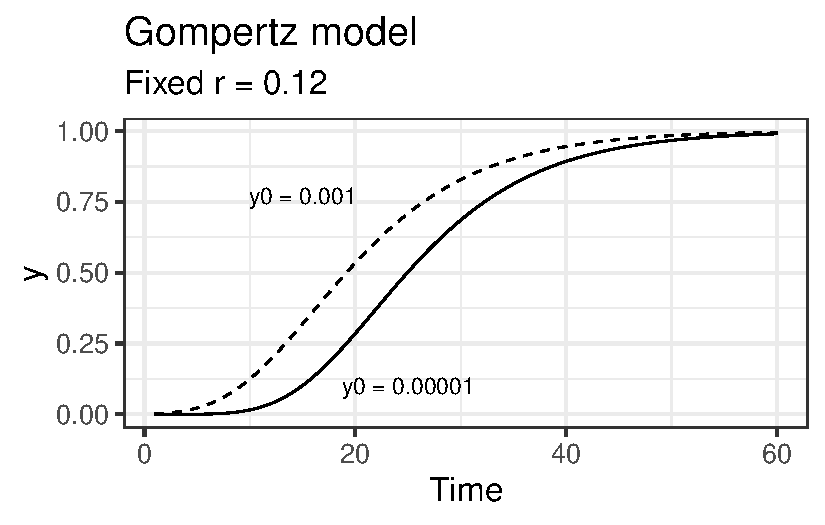
\includegraphics{./temporal-models_files/figure-pdf/unnamed-chunk-20-1.pdf}

}

\end{figure}

\hypertarget{model-fitting}{%
\chapter{Model fitting}\label{model-fitting}}

\begin{tcolorbox}[enhanced jigsaw, rightrule=.15mm, left=2mm, breakable, colframe=quarto-callout-note-color-frame, toprule=.15mm, leftrule=.75mm, bottomrule=.15mm, colback=white, arc=.35mm, opacityback=0]
\begin{minipage}[t]{5.5mm}
\textcolor{quarto-callout-note-color}{\faInfo}
\end{minipage}%
\begin{minipage}[t]{\textwidth - 5.5mm}
This is a work in progress that is currently undergoing heavy technical
editing and copy-editing\end{minipage}%
\end{tcolorbox}

In this tutorial, you will learn how to fit models to multiple actual
disease progress curves (DPCs) data obtained from the literature. I will
demonstrate how to fit and select the models using the \emph{epifitter}
package. A few user friendly functions will help us decide which model
to choose to obtain the parameters of interest and further compare the
epidemics.

To illustrate, I will use two datasets available from Chapter 3 from the
book, \emph{Study of Plant Disease Epidemics} (Madden et al. 2017b). In
the book, SAS codes are presented to perform a few analysis. We then
provide an alternative code for performing similar analysis, although
not perfectly reproducing the results from the book.

We will compare three DPCs of the incidence of tobacco etch, a virus
disease, in peppers. Evaluations of incidence were evaluated at a 7-day
interval, up to 49 days.The data are available in chapter 4 (page 93).
Let's input the data manually and create a data frame. First column is
the assessment time and the other columns correspond to the treatments,
called groups in the book, from 1 to 3.

\hypertarget{entering-data}{%
\subsection{Entering data}\label{entering-data}}

\begin{Shaded}
\begin{Highlighting}[]
\FunctionTok{library}\NormalTok{(tidyverse) }\CommentTok{\# essential packages }
\FunctionTok{library}\NormalTok{(cowplot) }\CommentTok{\# for themes }
\FunctionTok{theme\_set}\NormalTok{(}\FunctionTok{theme\_bw}\NormalTok{(}\AttributeTok{base\_size =} \DecValTok{16}\NormalTok{)) }\CommentTok{\# set global theme}
\end{Highlighting}
\end{Shaded}

\begin{Shaded}
\begin{Highlighting}[]
\NormalTok{pepper }\OtherTok{\textless{}{-}} 
  \FunctionTok{tribble}\NormalTok{(}
   \SpecialCharTok{\textasciitilde{}}\NormalTok{t,  }\SpecialCharTok{\textasciitilde{}}\StringTok{\textasciigrave{}}\AttributeTok{1}\StringTok{\textasciigrave{}}\NormalTok{,  }\SpecialCharTok{\textasciitilde{}}\StringTok{\textasciigrave{}}\AttributeTok{2}\StringTok{\textasciigrave{}}\NormalTok{,  }\SpecialCharTok{\textasciitilde{}}\StringTok{\textasciigrave{}}\AttributeTok{3}\StringTok{\textasciigrave{}}\NormalTok{,}
   \DecValTok{0}\NormalTok{,  }\FloatTok{0.08}\NormalTok{, }\FloatTok{0.001}\NormalTok{, }\FloatTok{0.001}\NormalTok{,}
   \DecValTok{7}\NormalTok{,  }\FloatTok{0.13}\NormalTok{,  }\FloatTok{0.01}\NormalTok{, }\FloatTok{0.001}\NormalTok{,}
  \DecValTok{14}\NormalTok{,  }\FloatTok{0.78}\NormalTok{,  }\FloatTok{0.09}\NormalTok{,  }\FloatTok{0.01}\NormalTok{,}
  \DecValTok{21}\NormalTok{,  }\FloatTok{0.92}\NormalTok{,  }\FloatTok{0.25}\NormalTok{,  }\FloatTok{0.05}\NormalTok{,}
  \DecValTok{28}\NormalTok{,  }\FloatTok{0.99}\NormalTok{,   }\FloatTok{0.8}\NormalTok{,  }\FloatTok{0.18}\NormalTok{,}
  \DecValTok{35}\NormalTok{, }\FloatTok{0.995}\NormalTok{,  }\FloatTok{0.98}\NormalTok{,  }\FloatTok{0.34}\NormalTok{,}
  \DecValTok{42}\NormalTok{, }\FloatTok{0.999}\NormalTok{,  }\FloatTok{0.99}\NormalTok{,  }\FloatTok{0.48}\NormalTok{,}
  \DecValTok{49}\NormalTok{, }\FloatTok{0.999}\NormalTok{, }\FloatTok{0.999}\NormalTok{,  }\FloatTok{0.74}
\NormalTok{  ) }
\end{Highlighting}
\end{Shaded}

\hypertarget{visualize-the-dpcs}{%
\subsection{Visualize the DPCs}\label{visualize-the-dpcs}}

Before proceeding with model selection and fitting, let's visualize the
three epidemics. The code below reproduces quite exactly the top plot of
Fig. 4.15 ((Madden et al. 2017b) page 94). The appraisal of the curves
might give us a hint on which models are the best candidates.

Because the data was entered in the wide format (each DPCs in a
different columns) we need to reshape it to the long format. The
\texttt{pivot\_longer} function will do the job of reshaping from wide
to long format so we can finally use the \texttt{ggplot} function to
produce the plot.

\begin{Shaded}
\begin{Highlighting}[]
\NormalTok{pepper }\SpecialCharTok{|\textgreater{}} 
  \FunctionTok{pivot\_longer}\NormalTok{(}\DecValTok{2}\SpecialCharTok{:}\DecValTok{4}\NormalTok{, }\AttributeTok{names\_to =}\StringTok{"treat"}\NormalTok{, }\AttributeTok{values\_to =} \StringTok{"inc"}\NormalTok{) }\SpecialCharTok{|\textgreater{}} 
  \FunctionTok{ggplot}\NormalTok{ (}\FunctionTok{aes}\NormalTok{(t, inc, }
              \AttributeTok{linetype =}\NormalTok{ treat, }
              \AttributeTok{shape =}\NormalTok{ treat, }
              \AttributeTok{group =}\NormalTok{ treat))}\SpecialCharTok{+}
  \FunctionTok{geom\_line}\NormalTok{(}\AttributeTok{size =} \DecValTok{1}\NormalTok{)}\SpecialCharTok{+}
  \FunctionTok{geom\_point}\NormalTok{(}\AttributeTok{size =}\DecValTok{3}\NormalTok{, }\AttributeTok{shape =} \DecValTok{16}\NormalTok{)}\SpecialCharTok{+}
  \FunctionTok{annotate}\NormalTok{(}\AttributeTok{geom =} \StringTok{"text"}\NormalTok{, }\AttributeTok{x =} \DecValTok{15}\NormalTok{, }\AttributeTok{y =} \FloatTok{0.84}\NormalTok{, }\AttributeTok{label =} \StringTok{"1"}\NormalTok{)}\SpecialCharTok{+}
  \FunctionTok{annotate}\NormalTok{(}\AttributeTok{geom =} \StringTok{"text"}\NormalTok{, }\AttributeTok{x =} \DecValTok{23}\NormalTok{, }\AttributeTok{y =} \FloatTok{0.6}\NormalTok{, }\AttributeTok{label =} \StringTok{"2"}\NormalTok{)}\SpecialCharTok{+}
  \FunctionTok{annotate}\NormalTok{(}\AttributeTok{geom =} \StringTok{"text"}\NormalTok{, }\AttributeTok{x =} \DecValTok{32}\NormalTok{, }\AttributeTok{y =} \FloatTok{0.33}\NormalTok{, }\AttributeTok{label =} \StringTok{"3"}\NormalTok{)}\SpecialCharTok{+}
  \FunctionTok{labs}\NormalTok{(}\AttributeTok{y =} \StringTok{"Disease incidence (y)"}\NormalTok{,}
       \AttributeTok{x =} \StringTok{"Time (days)"}\NormalTok{)}\SpecialCharTok{+}
  \FunctionTok{theme}\NormalTok{(}\AttributeTok{legend.position =} \StringTok{"none"}\NormalTok{)}
\end{Highlighting}
\end{Shaded}

\begin{figure}[H]

{\centering 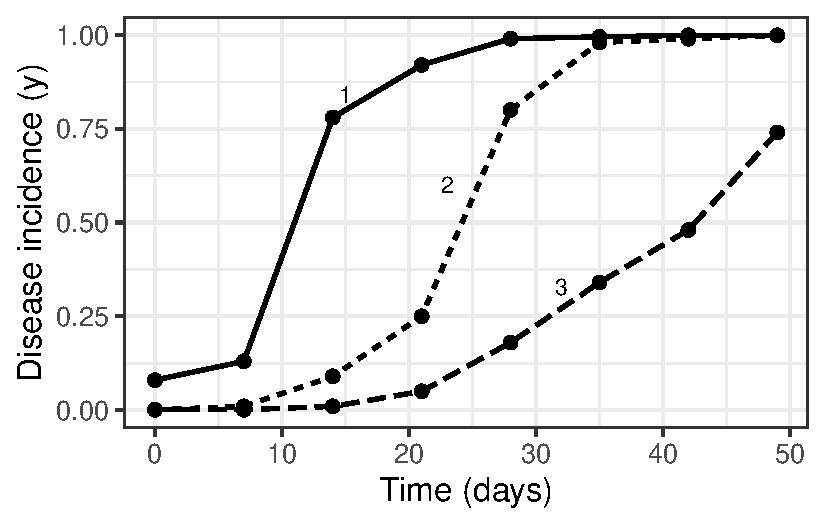
\includegraphics{./temporal-fitting_files/figure-pdf/unnamed-chunk-6-1.pdf}

}

\end{figure}

Most of the three curves show a sigmoid shape with the exception of
group 3 that resembles an exponential growth, not reaching the maximum
value, and thus suggesting an incomplete epidemic. We can easily
eliminate the monomolecular and exponential models and decide on the
other two non-flexible models: logistic or Gompertz. To do that, let's
proceed to model fitting and evaluate the statistics for supporting a
final decision. There are two modeling approaches for model fitting in
epifitter: the \textbf{linear} or \textbf{nonlinear}
parameter-estimation methods.

\hypertarget{fitting-single-epidemics}{%
\subsection{Fitting: single epidemics}\label{fitting-single-epidemics}}

Among the several options offered by \emph{epifitter} we start with the
simplest one, which is fit a model to a single epidemics using the
linear regression approach. For such, the \texttt{fit\_lin()} requires
two arguments: time (\texttt{time}) and disease intensity (\texttt{y})
each one as a vector stored or not in a dataframe.

Since we have three epidemics, \texttt{fit\_lin()} will be use three
times. The function produces a list object with six elements. Let's
first look at the \texttt{Stats} dataframe of each of the three lists
named \texttt{epi1} to \texttt{epi3}.

\begin{Shaded}
\begin{Highlighting}[]
\FunctionTok{library}\NormalTok{(epifitter)}
\NormalTok{epi1 }\OtherTok{\textless{}{-}} \FunctionTok{fit\_lin}\NormalTok{(}\AttributeTok{time =}\NormalTok{ pepper}\SpecialCharTok{$}\NormalTok{t,  }
                \AttributeTok{y =}\NormalTok{ pepper}\SpecialCharTok{$}\StringTok{\textasciigrave{}}\AttributeTok{1}\StringTok{\textasciigrave{}}\NormalTok{ )}
\NormalTok{epi1}\SpecialCharTok{$}\NormalTok{Stats}
\end{Highlighting}
\end{Shaded}

\begin{verbatim}
                 CCC r_squared    RSE
Gompertz      0.9848    0.9700 0.5911
Monomolecular 0.9838    0.9681 0.5432
Logistic      0.9782    0.9572 0.8236
Exponential   0.7839    0.6447 0.6705
\end{verbatim}

\begin{Shaded}
\begin{Highlighting}[]
\NormalTok{epi2 }\OtherTok{\textless{}{-}} \FunctionTok{fit\_lin}\NormalTok{(}\AttributeTok{time =}\NormalTok{ pepper}\SpecialCharTok{$}\NormalTok{t,  }
  \AttributeTok{y =}\NormalTok{ pepper}\SpecialCharTok{$}\StringTok{\textasciigrave{}}\AttributeTok{2}\StringTok{\textasciigrave{}}\NormalTok{ )}
\NormalTok{epi2}\SpecialCharTok{$}\NormalTok{Stats}
\end{Highlighting}
\end{Shaded}

\begin{verbatim}
                 CCC r_squared    RSE
Logistic      0.9962    0.9924 0.4524
Gompertz      0.9707    0.9431 0.8408
Monomolecular 0.9248    0.8601 1.0684
Exponential   0.8971    0.8134 1.2016
\end{verbatim}

\begin{Shaded}
\begin{Highlighting}[]
\NormalTok{epi3 }\OtherTok{\textless{}{-}} \FunctionTok{fit\_lin}\NormalTok{(}\AttributeTok{time =}\NormalTok{ pepper}\SpecialCharTok{$}\NormalTok{t,  }
  \AttributeTok{y =}\NormalTok{ pepper}\SpecialCharTok{$}\StringTok{\textasciigrave{}}\AttributeTok{3}\StringTok{\textasciigrave{}}\NormalTok{ )}
\NormalTok{epi3}\SpecialCharTok{$}\NormalTok{Stats}
\end{Highlighting}
\end{Shaded}

\begin{verbatim}
                 CCC r_squared    RSE
Logistic      0.9829    0.9665 0.6045
Gompertz      0.9825    0.9656 0.2263
Exponential   0.9636    0.9297 0.7706
Monomolecular 0.8592    0.7531 0.2534
\end{verbatim}

The statistics of the model fit confirms our initial guess that the
predictions by the logistic or the Gompertz are closer to the
observations than predictions by the other models. There is no much
difference between them based on these statistics. However, to pick one
of the models, it is important to inspect the curves with the observed
and predicted values to check which model is best for all curves.

\hypertarget{fitting-multiple-epidemics}{%
\subsection{Fitting: multiple
epidemics}\label{fitting-multiple-epidemics}}

Before looking at the prediction, let's use another handy function that
allows us to simultaneously fit the models to multiple DPC data.
Different from \texttt{fit\_lin()}, \texttt{fit\_multi()} requires the
data to be structured in the long format where there is a column
specifying each of the epidemics.

Let's then create a new data set called \texttt{pepper2} using the data
transposing functions of the \emph{tidyr} package.

\begin{Shaded}
\begin{Highlighting}[]
\NormalTok{pepper2 }\OtherTok{\textless{}{-}}\NormalTok{ pepper }\SpecialCharTok{|\textgreater{}} 
  \FunctionTok{pivot\_longer}\NormalTok{(}\DecValTok{2}\SpecialCharTok{:}\DecValTok{4}\NormalTok{, }\AttributeTok{names\_to =}\StringTok{"treat"}\NormalTok{, }\AttributeTok{values\_to =} \StringTok{"inc"}\NormalTok{)}
\end{Highlighting}
\end{Shaded}

Now we fit the models to all DPCs. Note that the name of the variable
indicating the DPC code needs to be informed in \texttt{strata\_cols}
argument.

\begin{Shaded}
\begin{Highlighting}[]
\NormalTok{epi\_all }\OtherTok{\textless{}{-}} \FunctionTok{fit\_multi}\NormalTok{(}
  \AttributeTok{time\_col =} \StringTok{"t"}\NormalTok{,}
  \AttributeTok{intensity\_col =} \StringTok{"inc"}\NormalTok{,}
  \AttributeTok{data =}\NormalTok{ pepper2,}
  \AttributeTok{strata\_cols =} \StringTok{"treat"}\NormalTok{,}
  \AttributeTok{nlin =} \ConstantTok{FALSE}
\NormalTok{)}
\end{Highlighting}
\end{Shaded}

Now let's select the statistics of model fitting. Again,
\emph{Epifitter} ranks the models based on the CCC (the higher the
better) but it is important to check the RSE as well - the lower the
better. In fact, the RSE is more important when the goal is prediction.

\begin{Shaded}
\begin{Highlighting}[]
\NormalTok{epi\_all}\SpecialCharTok{$}\NormalTok{Parameters }\SpecialCharTok{|\textgreater{}} 
  \FunctionTok{select}\NormalTok{(treat, model, best\_model, RSE, CCC)}
\end{Highlighting}
\end{Shaded}

\begin{verbatim}
   treat         model best_model       RSE       CCC
1      1      Gompertz          1 0.5911056 0.9847857
2      1 Monomolecular          2 0.5431977 0.9838044
3      1      Logistic          3 0.8235798 0.9781534
4      1   Exponential          4 0.6705085 0.7839381
5      2      Logistic          1 0.4523616 0.9961683
6      2      Gompertz          2 0.8407922 0.9707204
7      2 Monomolecular          3 1.0683633 0.9247793
8      2   Exponential          4 1.2015809 0.8971003
9      3      Logistic          1 0.6045243 0.9829434
10     3      Gompertz          2 0.2262550 0.9824935
11     3   Exponential          3 0.7705736 0.9635747
12     3 Monomolecular          4 0.2533763 0.8591837
\end{verbatim}

To be more certain about our decision, let's advance to the final step
which is to produce the plots with the observed and predicted values for
each assessment time by calling the \texttt{Data} dataframe of the
`\texttt{epi\_all} list.

\begin{Shaded}
\begin{Highlighting}[]
\NormalTok{epi\_all}\SpecialCharTok{$}\NormalTok{Data }\SpecialCharTok{|\textgreater{}}
 \FunctionTok{filter}\NormalTok{(model }\SpecialCharTok{\%in\%} \FunctionTok{c}\NormalTok{(}\StringTok{"Gompertz"}\NormalTok{, }\StringTok{"Logistic"}\NormalTok{)) }\SpecialCharTok{|\textgreater{}} 
  \FunctionTok{ggplot}\NormalTok{(}\FunctionTok{aes}\NormalTok{(time, predicted, }\AttributeTok{shape =}\NormalTok{ treat)) }\SpecialCharTok{+}
  \FunctionTok{geom\_point}\NormalTok{(}\FunctionTok{aes}\NormalTok{(time, y)) }\SpecialCharTok{+}
  \FunctionTok{geom\_line}\NormalTok{() }\SpecialCharTok{+}
  \FunctionTok{facet\_wrap}\NormalTok{(}\SpecialCharTok{\textasciitilde{}}\NormalTok{ model) }\SpecialCharTok{+}
 \FunctionTok{coord\_cartesian}\NormalTok{(}\AttributeTok{ylim =} \FunctionTok{c}\NormalTok{(}\DecValTok{0}\NormalTok{, }\DecValTok{1}\NormalTok{)) }\SpecialCharTok{+} \CommentTok{\# set the max to 0.6}
  \FunctionTok{labs}\NormalTok{(}
    \AttributeTok{y =} \StringTok{"Disease incidence"}\NormalTok{,}
    \AttributeTok{x =} \StringTok{"Time (days after emergence)"}
\NormalTok{  )}
\end{Highlighting}
\end{Shaded}

\begin{figure}[H]

{\centering 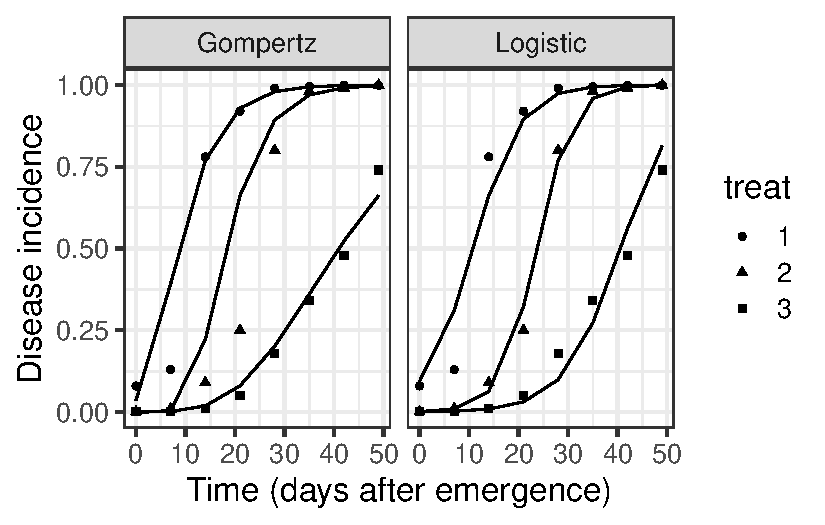
\includegraphics{./temporal-fitting_files/figure-pdf/unnamed-chunk-20-1.pdf}

}

\end{figure}

Overall, the logistic model seems a better fit for all the curves. Let's
produce a plot with the prediction error versus time.

\begin{Shaded}
\begin{Highlighting}[]
\NormalTok{epi\_all}\SpecialCharTok{$}\NormalTok{Data }\SpecialCharTok{|\textgreater{}}
 \FunctionTok{filter}\NormalTok{(model }\SpecialCharTok{\%in\%} \FunctionTok{c}\NormalTok{(}\StringTok{"Gompertz"}\NormalTok{, }\StringTok{"Logistic"}\NormalTok{)) }\SpecialCharTok{|\textgreater{}} 
  \FunctionTok{ggplot}\NormalTok{(}\FunctionTok{aes}\NormalTok{(time, predicted }\SpecialCharTok{{-}}\NormalTok{y, }\AttributeTok{shape =}\NormalTok{ treat)) }\SpecialCharTok{+}
  \FunctionTok{geom\_point}\NormalTok{() }\SpecialCharTok{+}
  \FunctionTok{geom\_line}\NormalTok{() }\SpecialCharTok{+}
  \FunctionTok{geom\_hline}\NormalTok{(}\AttributeTok{yintercept =} \DecValTok{0}\NormalTok{, }\AttributeTok{linetype =}\DecValTok{2}\NormalTok{)}\SpecialCharTok{+}
  \FunctionTok{facet\_wrap}\NormalTok{(}\SpecialCharTok{\textasciitilde{}}\NormalTok{ model) }\SpecialCharTok{+}
 \FunctionTok{coord\_cartesian}\NormalTok{(}\AttributeTok{ylim =} \FunctionTok{c}\NormalTok{(}\SpecialCharTok{{-}}\FloatTok{0.4}\NormalTok{, }\FloatTok{0.4}\NormalTok{)) }\SpecialCharTok{+} \CommentTok{\# set the max to 0.6}
  \FunctionTok{labs}\NormalTok{(}
    \AttributeTok{y =} \StringTok{"Prediction error"}\NormalTok{,}
    \AttributeTok{x =} \StringTok{"Time (days after emergence)"}
\NormalTok{  )}
\end{Highlighting}
\end{Shaded}

\begin{figure}[H]

{\centering 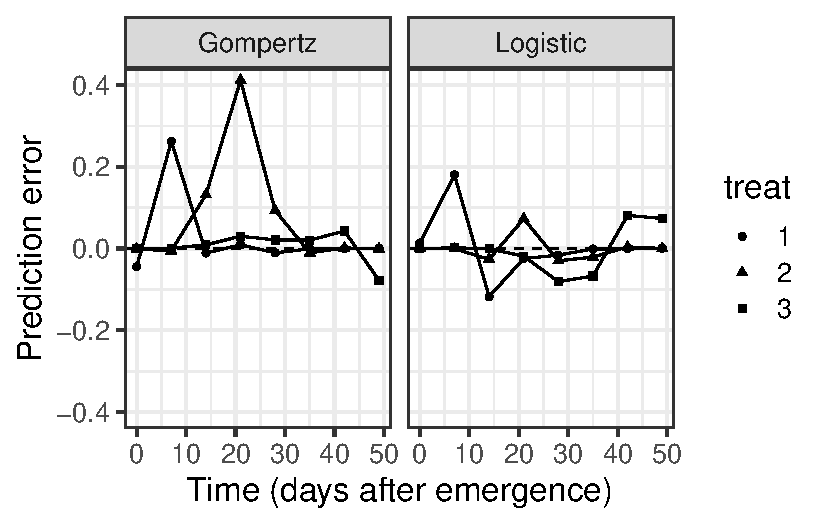
\includegraphics{./temporal-fitting_files/figure-pdf/unnamed-chunk-22-1.pdf}

}

\end{figure}

The plots above confirms the logistic model as good fit overall because
the errors for all epidemics combined are more scattered around the
non-error line.

\begin{Shaded}
\begin{Highlighting}[]
\NormalTok{  epi\_all}\SpecialCharTok{$}\NormalTok{Parameters }\SpecialCharTok{|\textgreater{}}
    \FunctionTok{filter}\NormalTok{(model }\SpecialCharTok{==} \StringTok{"Logistic"}\NormalTok{) }\SpecialCharTok{|\textgreater{}}
    \FunctionTok{select}\NormalTok{(treat, y0, y0\_ci\_lwr, y0\_ci\_upr, r, r\_ci\_lwr, r\_ci\_upr }
\NormalTok{)}
\end{Highlighting}
\end{Shaded}

\begin{verbatim}
  treat           y0    y0_ci_lwr   y0_ci_upr         r  r_ci_lwr  r_ci_upr
1     1 0.0935037690 0.0273207272 0.274728744 0.2104047 0.1659824 0.2548270
2     2 0.0013727579 0.0006723537 0.002800742 0.2784814 0.2540818 0.3028809
3     3 0.0008132926 0.0003131745 0.002110379 0.1752146 0.1426077 0.2078215
\end{verbatim}

We can produce a plot for visual inference on the differences in the
parameters.

\begin{Shaded}
\begin{Highlighting}[]
\NormalTok{p1 }\OtherTok{\textless{}{-}}\NormalTok{ epi\_all}\SpecialCharTok{$}\NormalTok{Parameters }\SpecialCharTok{|\textgreater{}}
  \FunctionTok{filter}\NormalTok{(model }\SpecialCharTok{==} \StringTok{"Logistic"}\NormalTok{) }\SpecialCharTok{|\textgreater{}}
  \FunctionTok{ggplot}\NormalTok{(}\FunctionTok{aes}\NormalTok{(treat, r)) }\SpecialCharTok{+}
  \FunctionTok{geom\_point}\NormalTok{(}\AttributeTok{size =} \DecValTok{3}\NormalTok{) }\SpecialCharTok{+}
  \FunctionTok{geom\_errorbar}\NormalTok{(}\FunctionTok{aes}\NormalTok{(}\AttributeTok{ymin =}\NormalTok{ r\_ci\_lwr, }\AttributeTok{ymax =}\NormalTok{ r\_ci\_upr),}
    \AttributeTok{width =} \DecValTok{0}\NormalTok{,}
    \AttributeTok{size =} \DecValTok{1}
\NormalTok{  ) }\SpecialCharTok{+}
  \FunctionTok{labs}\NormalTok{(}
    \AttributeTok{x =} \StringTok{"Time"}\NormalTok{,}
    \AttributeTok{y =} \StringTok{"r"}
\NormalTok{  )}

\NormalTok{p2 }\OtherTok{\textless{}{-}}\NormalTok{ epi\_all}\SpecialCharTok{$}\NormalTok{Parameters }\SpecialCharTok{|\textgreater{}}
  \FunctionTok{filter}\NormalTok{(model }\SpecialCharTok{==} \StringTok{"Logistic"}\NormalTok{) }\SpecialCharTok{|\textgreater{}}
  \FunctionTok{ggplot}\NormalTok{(}\FunctionTok{aes}\NormalTok{(treat, }\DecValTok{1} \SpecialCharTok{{-}} \FunctionTok{exp}\NormalTok{(}\SpecialCharTok{{-}}\NormalTok{y0))) }\SpecialCharTok{+}
  \FunctionTok{geom\_point}\NormalTok{(}\AttributeTok{size =} \DecValTok{3}\NormalTok{) }\SpecialCharTok{+}
  \FunctionTok{geom\_errorbar}\NormalTok{(}\FunctionTok{aes}\NormalTok{(}\AttributeTok{ymin =}\NormalTok{ y0\_ci\_lwr, }\AttributeTok{ymax =}\NormalTok{ y0\_ci\_upr),}
    \AttributeTok{width =} \DecValTok{0}\NormalTok{,}
    \AttributeTok{size =} \DecValTok{1}
\NormalTok{  ) }\SpecialCharTok{+}
  \FunctionTok{labs}\NormalTok{(}
    \AttributeTok{x =} \StringTok{"Time"}\NormalTok{,}
    \AttributeTok{y =} \StringTok{"y0"}
\NormalTok{  )}

\FunctionTok{library}\NormalTok{(patchwork)}
\end{Highlighting}
\end{Shaded}

\begin{verbatim}

Attaching package: 'patchwork'
\end{verbatim}

\begin{verbatim}
The following object is masked from 'package:cowplot':

    align_plots
\end{verbatim}

\begin{Shaded}
\begin{Highlighting}[]
\NormalTok{p1 }\SpecialCharTok{|}\NormalTok{ p2}
\end{Highlighting}
\end{Shaded}

\begin{figure}[H]

{\centering 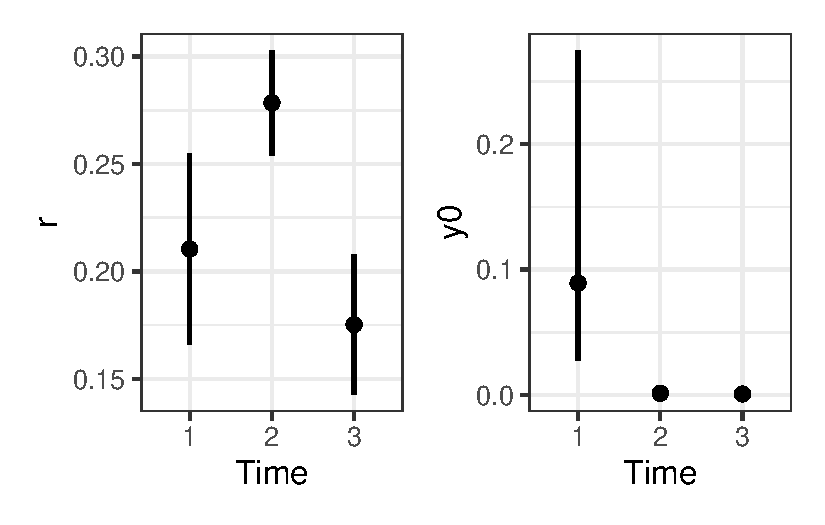
\includegraphics{./temporal-fitting_files/figure-pdf/unnamed-chunk-26-1.pdf}

}

\end{figure}

\hypertarget{designed-experiments}{%
\subsection{Designed experiments}\label{designed-experiments}}

In this next section, we will work with disease data collected over time
in the same plot unit (also called repeated measures) from a designed
experiment for evaluating and comparing treatment effects.

Again, we will use a dataset of progress curves shown in page 98 (Madden
et al. 2017b). The curves represent the incidence of soybean plants
symptomatic for bud blight caused by tobacco streak virus. Four
treatments (different planting dates) were evaluated in randomized
complete block design with four replicates. There are four assessment in
time for each curve. The data was stored as a csv file and will be
loaded using \texttt{read\_csv()} function and stored as dataframe
called \texttt{budblight}.

\hypertarget{loading-data}{%
\subsubsection{Loading data}\label{loading-data}}

\begin{Shaded}
\begin{Highlighting}[]
\NormalTok{budblight }\OtherTok{\textless{}{-}} \FunctionTok{read\_csv}\NormalTok{(}\StringTok{"https://raw.githubusercontent.com/emdelponte/epidemiology{-}R/main/data/bud{-}blight{-}soybean.csv"}\NormalTok{)}
\end{Highlighting}
\end{Shaded}

\begin{verbatim}
Rows: 64 Columns: 4
-- Column specification --------------------------------------------------------
Delimiter: ","
chr (1): treat
dbl (3): time, block, y

i Use `spec()` to retrieve the full column specification for this data.
i Specify the column types or set `show_col_types = FALSE` to quiet this message.
\end{verbatim}

Let's have a look at the first six rows of the dataset and check the
data type for each column. There is an additional column representing
the replicates, called block.

\begin{Shaded}
\begin{Highlighting}[]
\FunctionTok{head}\NormalTok{(budblight)}
\end{Highlighting}
\end{Shaded}

\begin{verbatim}
# A tibble: 6 x 4
  treat  time block     y
  <chr> <dbl> <dbl> <dbl>
1 PD1      30     1  0.1 
2 PD1      30     2  0.3 
3 PD1      30     3  0.1 
4 PD1      30     4  0.1 
5 PD1      40     1  0.3 
6 PD1      40     2  0.38
\end{verbatim}

\hypertarget{visualizing-the-dpcs}{%
\subsubsection{Visualizing the DPCs}\label{visualizing-the-dpcs}}

Let's have a look at the curves and produce a combo plot figure similar
to Fig. 4.17 of the book, but without the line of the predicted values.

\begin{Shaded}
\begin{Highlighting}[]
\NormalTok{p3 }\OtherTok{\textless{}{-}}\NormalTok{ budblight }\SpecialCharTok{|\textgreater{}}
  \FunctionTok{ggplot}\NormalTok{(}\FunctionTok{aes}\NormalTok{(}
\NormalTok{    time, y,}
    \AttributeTok{group =}\NormalTok{ block,}
    \AttributeTok{shape =} \FunctionTok{factor}\NormalTok{(block)}
\NormalTok{  )) }\SpecialCharTok{+}
  \FunctionTok{geom\_point}\NormalTok{(}\AttributeTok{size =} \FloatTok{1.5}\NormalTok{) }\SpecialCharTok{+}
  \FunctionTok{ylim}\NormalTok{(}\DecValTok{0}\NormalTok{, }\FloatTok{0.6}\NormalTok{) }\SpecialCharTok{+}
  \FunctionTok{theme}\NormalTok{(}\AttributeTok{legend.position =} \StringTok{"none"}\NormalTok{)}\SpecialCharTok{+}
  \FunctionTok{facet\_wrap}\NormalTok{(}\SpecialCharTok{\textasciitilde{}}\NormalTok{treat, }\AttributeTok{ncol =}\DecValTok{1}\NormalTok{)}\SpecialCharTok{+}
  \FunctionTok{labs}\NormalTok{(}\AttributeTok{y =} \StringTok{"Disease incidence"}\NormalTok{,}
       \AttributeTok{x =} \StringTok{"Time (days after emergence)"}\NormalTok{)}
\end{Highlighting}
\end{Shaded}

\begin{Shaded}
\begin{Highlighting}[]
\NormalTok{p4 }\OtherTok{\textless{}{-}}\NormalTok{ budblight }\SpecialCharTok{|\textgreater{}}
  \FunctionTok{ggplot}\NormalTok{(}\FunctionTok{aes}\NormalTok{(}
\NormalTok{    time, }\FunctionTok{log}\NormalTok{(}\DecValTok{1} \SpecialCharTok{/}\NormalTok{ (}\DecValTok{1} \SpecialCharTok{{-}}\NormalTok{ y)),}
    \AttributeTok{group =}\NormalTok{ block,}
    \AttributeTok{shape =} \FunctionTok{factor}\NormalTok{(block)}
\NormalTok{  )) }\SpecialCharTok{+}
  \FunctionTok{geom\_point}\NormalTok{(}\AttributeTok{size =} \DecValTok{2}\NormalTok{) }\SpecialCharTok{+}
  \FunctionTok{facet\_wrap}\NormalTok{(}\SpecialCharTok{\textasciitilde{}}\NormalTok{treat, }\AttributeTok{ncol =} \DecValTok{1}\NormalTok{) }\SpecialCharTok{+}
  \FunctionTok{theme}\NormalTok{(}\AttributeTok{legend.position =} \StringTok{"none"}\NormalTok{)}\SpecialCharTok{+}
  \FunctionTok{labs}\NormalTok{(}\AttributeTok{y =} \StringTok{"Transformed incidence"}\NormalTok{, }\AttributeTok{x =} \StringTok{"Time (days after emergence)"}\NormalTok{)}

\NormalTok{p3 }\SpecialCharTok{|}\NormalTok{ p4}
\end{Highlighting}
\end{Shaded}

\begin{figure}[H]

{\centering 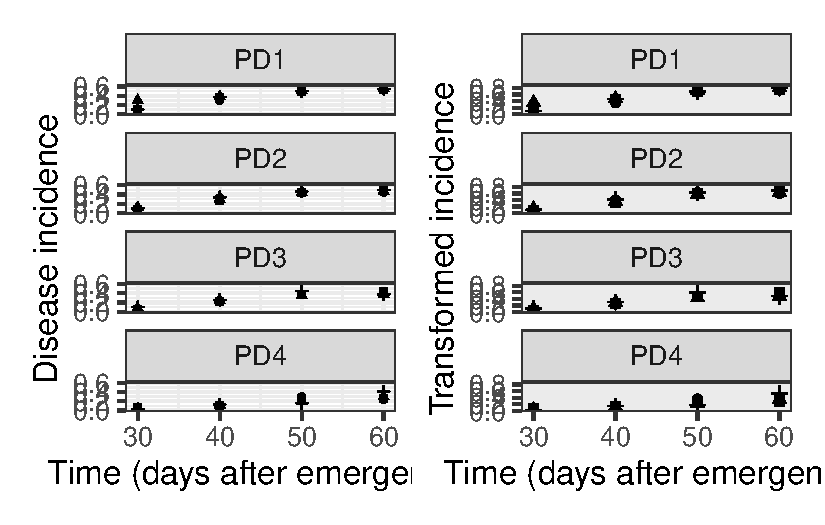
\includegraphics{./temporal-fitting_files/figure-pdf/unnamed-chunk-34-1.pdf}

}

\end{figure}

\hypertarget{model-fitting-1}{%
\subsubsection{Model fitting}\label{model-fitting-1}}

Remember that the first step in model selection is the visual appraisal
of the curve data linearized with the model transformation. In the case
the curves represent complete epidemics (close to 100\%) appraisal of
the absolute rate (difference in y between two times) over time is also
helpful.

For the treatments above, it looks like the curves are typical of a
monocyclic disease (the case of soybean bud blight), for which the
monomolecular is usually a good fit, but other models are also possible
as well. For this exercise, we will use both the linear and the
nonlinear estimation method.

\hypertarget{linear-regression}{%
\paragraph{Linear regression}\label{linear-regression}}

For convenience, we use the \texttt{fit\_multi()} to handle multiple
epidemics. The function returns a list object where a series of
statistics are provided to aid in model selection and parameter
estimation. We need to provide the names of columns (arguments):
assessment time (\texttt{time\_col}), disease incidence
(\texttt{intensity\_col}), and treatment (\texttt{strata\_cols}).

\begin{Shaded}
\begin{Highlighting}[]
\NormalTok{lin1 }\OtherTok{\textless{}{-}} \FunctionTok{fit\_multi}\NormalTok{(}
  \AttributeTok{time\_col =} \StringTok{"time"}\NormalTok{,}
  \AttributeTok{intensity\_col =} \StringTok{"y"}\NormalTok{,}
  \AttributeTok{data =}\NormalTok{ budblight,}
  \AttributeTok{strata\_cols =} \StringTok{"treat"}\NormalTok{,}
  \AttributeTok{nlin =} \ConstantTok{FALSE}
\NormalTok{)}
\end{Highlighting}
\end{Shaded}

Let's look at how well the four models fitted the data. Epifitter
suggests the best fitted model (1 to 4, where 1 is best) for each
treatment. Let's have a look at the statistics of model fitting.

\begin{Shaded}
\begin{Highlighting}[]
\NormalTok{  lin1}\SpecialCharTok{$}\NormalTok{Parameters }\SpecialCharTok{|\textgreater{}} 
    \FunctionTok{select}\NormalTok{(treat, best\_model, model, CCC, RSE)}
\end{Highlighting}
\end{Shaded}

\begin{verbatim}
   treat best_model         model       CCC        RSE
1    PD1          1 Monomolecular 0.9348429 0.09805661
2    PD1          2      Gompertz 0.9040182 0.22226189
3    PD1          3      Logistic 0.8711178 0.44751963
4    PD1          4   Exponential 0.8278055 0.36124036
5    PD2          1 Monomolecular 0.9547434 0.07003116
6    PD2          2      Gompertz 0.9307192 0.17938711
7    PD2          3      Logistic 0.9062012 0.38773023
8    PD2          4   Exponential 0.8796705 0.32676216
9    PD3          1 Monomolecular 0.9393356 0.06832499
10   PD3          2      Gompertz 0.9288436 0.17156394
11   PD3          3      Logistic 0.9085414 0.39051075
12   PD3          4   Exponential 0.8896173 0.33884790
13   PD4          1      Gompertz 0.9234736 0.17474422
14   PD4          2 Monomolecular 0.8945962 0.06486949
15   PD4          3      Logistic 0.8911344 0.52412586
16   PD4          4   Exponential 0.8739618 0.49769642
\end{verbatim}

And now we extract values for each parameter estimated from the fit of
the monomolecular model.

\begin{Shaded}
\begin{Highlighting}[]
\NormalTok{  lin1}\SpecialCharTok{$}\NormalTok{Parameters }\SpecialCharTok{|\textgreater{}}
  \FunctionTok{filter}\NormalTok{(model }\SpecialCharTok{==} \StringTok{"Monomolecular"}\NormalTok{) }\SpecialCharTok{|\textgreater{}}
  \FunctionTok{select}\NormalTok{(treat, y0, r)}
\end{Highlighting}
\end{Shaded}

\begin{verbatim}
  treat         y0          r
1   PD1 -0.5727700 0.02197351
2   PD2 -0.5220593 0.01902952
3   PD3 -0.4491365 0.01590586
4   PD4 -0.3619898 0.01118047
\end{verbatim}

Now we visualize the fit of the monomolecular model (using
\texttt{filter} function - see below) to the data together with the
observed data and then reproduce the right plots in Fig. 4.17 from the
book.

\begin{Shaded}
\begin{Highlighting}[]
\NormalTok{lin1}\SpecialCharTok{$}\NormalTok{Data }\SpecialCharTok{|\textgreater{}}
  \FunctionTok{filter}\NormalTok{(model }\SpecialCharTok{==} \StringTok{"Monomolecular"}\NormalTok{) }\SpecialCharTok{|\textgreater{}}
  \FunctionTok{ggplot}\NormalTok{(}\FunctionTok{aes}\NormalTok{(time, predicted)) }\SpecialCharTok{+}
  \FunctionTok{geom\_point}\NormalTok{(}\FunctionTok{aes}\NormalTok{(time, y)) }\SpecialCharTok{+}
  \FunctionTok{geom\_line}\NormalTok{(}\AttributeTok{size =} \FloatTok{0.5}\NormalTok{) }\SpecialCharTok{+}
  \FunctionTok{facet\_wrap}\NormalTok{(}\SpecialCharTok{\textasciitilde{}}\NormalTok{treat) }\SpecialCharTok{+}
  \FunctionTok{coord\_cartesian}\NormalTok{(}\AttributeTok{ylim =} \FunctionTok{c}\NormalTok{(}\DecValTok{0}\NormalTok{, }\FloatTok{0.6}\NormalTok{)) }\SpecialCharTok{+} \CommentTok{\# set the max to 0.6}
  \FunctionTok{labs}\NormalTok{(}
    \AttributeTok{y =} \StringTok{"Disease incidence"}\NormalTok{,}
    \AttributeTok{x =} \StringTok{"Time (days after emergence)"}
\NormalTok{  )}
\end{Highlighting}
\end{Shaded}

\begin{figure}[H]

{\centering 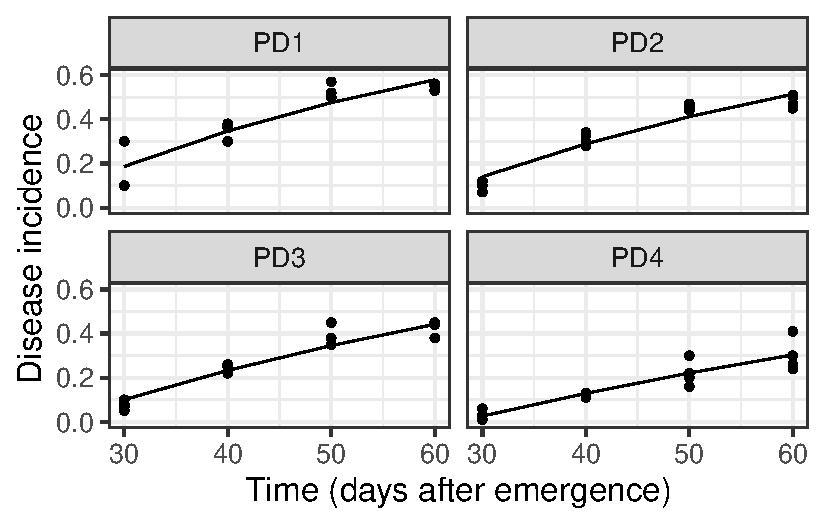
\includegraphics{./temporal-fitting_files/figure-pdf/unnamed-chunk-42-1.pdf}

}

\end{figure}

Now we can plot the means and respective 95\% confidence interval of the
apparent infection rate (\(r\)) and initial inoculum (\(y_0\)) for
visual inference.

\begin{Shaded}
\begin{Highlighting}[]
\NormalTok{p5 }\OtherTok{\textless{}{-}}\NormalTok{ lin1}\SpecialCharTok{$}\NormalTok{Parameters }\SpecialCharTok{|\textgreater{}}
  \FunctionTok{filter}\NormalTok{(model }\SpecialCharTok{==} \StringTok{"Monomolecular"}\NormalTok{) }\SpecialCharTok{|\textgreater{}}
  \FunctionTok{ggplot}\NormalTok{(}\FunctionTok{aes}\NormalTok{(treat, r)) }\SpecialCharTok{+}
  \FunctionTok{geom\_point}\NormalTok{(}\AttributeTok{size =} \DecValTok{3}\NormalTok{) }\SpecialCharTok{+}
  \FunctionTok{geom\_errorbar}\NormalTok{(}\FunctionTok{aes}\NormalTok{(}\AttributeTok{ymin =}\NormalTok{ r\_ci\_lwr, }\AttributeTok{ymax =}\NormalTok{ r\_ci\_upr),}
    \AttributeTok{width =} \DecValTok{0}\NormalTok{,}
    \AttributeTok{size =} \DecValTok{1}
\NormalTok{  ) }\SpecialCharTok{+}
  \FunctionTok{labs}\NormalTok{(}
    \AttributeTok{x =} \StringTok{"Time"}\NormalTok{,}
    \AttributeTok{y =} \StringTok{"r"}
\NormalTok{  )}

\NormalTok{p6 }\OtherTok{\textless{}{-}}\NormalTok{ lin1}\SpecialCharTok{$}\NormalTok{Parameters }\SpecialCharTok{|\textgreater{}}
  \FunctionTok{filter}\NormalTok{(model }\SpecialCharTok{==} \StringTok{"Monomolecular"}\NormalTok{) }\SpecialCharTok{|\textgreater{}}
  \FunctionTok{ggplot}\NormalTok{(}\FunctionTok{aes}\NormalTok{(treat, }\DecValTok{1} \SpecialCharTok{{-}} \FunctionTok{exp}\NormalTok{(}\SpecialCharTok{{-}}\NormalTok{y0))) }\SpecialCharTok{+}
  \FunctionTok{geom\_point}\NormalTok{(}\AttributeTok{size =} \DecValTok{3}\NormalTok{) }\SpecialCharTok{+}
  \FunctionTok{geom\_errorbar}\NormalTok{(}\FunctionTok{aes}\NormalTok{(}\AttributeTok{ymin =}\NormalTok{ y0\_ci\_lwr, }\AttributeTok{ymax =}\NormalTok{ y0\_ci\_upr),}
    \AttributeTok{width =} \DecValTok{0}\NormalTok{,}
    \AttributeTok{size =} \DecValTok{1}
\NormalTok{  ) }\SpecialCharTok{+}
  \FunctionTok{labs}\NormalTok{(}
    \AttributeTok{x =} \StringTok{"Time"}\NormalTok{,}
    \AttributeTok{y =} \StringTok{"y0"}
\NormalTok{  )}

\NormalTok{p5 }\SpecialCharTok{|}\NormalTok{ p2}
\end{Highlighting}
\end{Shaded}

\begin{figure}[H]

{\centering 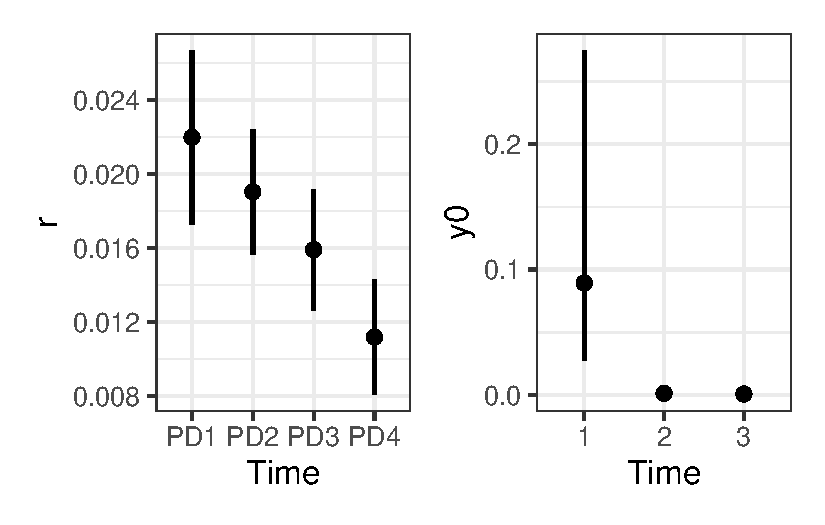
\includegraphics{./temporal-fitting_files/figure-pdf/unnamed-chunk-44-1.pdf}

}

\end{figure}

\hypertarget{non-linear-regression}{%
\paragraph{Non-linear regression}\label{non-linear-regression}}

To estimate the parameters using the non-linear approach, we repeat the
same arguments in the \texttt{fit\_multi} function, but include an
additional argument \texttt{nlin} set to \texttt{TRUE}.

\begin{Shaded}
\begin{Highlighting}[]
\NormalTok{nlin1 }\OtherTok{\textless{}{-}} \FunctionTok{fit\_multi}\NormalTok{(}
  \AttributeTok{time\_col =} \StringTok{"time"}\NormalTok{,}
  \AttributeTok{intensity\_col =} \StringTok{"y"}\NormalTok{,}
  \AttributeTok{data =}\NormalTok{ budblight,}
  \AttributeTok{strata\_cols =} \StringTok{"treat"}\NormalTok{,}
  \AttributeTok{nlin =} \ConstantTok{TRUE}
\NormalTok{)}
\end{Highlighting}
\end{Shaded}

\begin{verbatim}
Warning in log(y0/1): NaNs produced

Warning in log(y0/1): NaNs produced

Warning in log(y0/1): NaNs produced
\end{verbatim}

Let's check statistics of model fit.

\begin{Shaded}
\begin{Highlighting}[]
\NormalTok{nlin1}\SpecialCharTok{$}\NormalTok{Parameters }\SpecialCharTok{|\textgreater{}}
  \FunctionTok{select}\NormalTok{(treat, model, CCC, RSE, best\_model)}
\end{Highlighting}
\end{Shaded}

\begin{verbatim}
   treat         model       CCC        RSE best_model
1    PD1 Monomolecular 0.9382991 0.06133704          1
2    PD1      Gompertz 0.9172407 0.06986307          2
3    PD1      Logistic 0.8957351 0.07700720          3
4    PD1   Exponential 0.8544194 0.08799512          4
5    PD2 Monomolecular 0.9667886 0.04209339          1
6    PD2      Gompertz 0.9348370 0.05726761          2
7    PD2      Logistic 0.9077857 0.06657793          3
8    PD2   Exponential 0.8702365 0.07667322          4
9    PD3 Monomolecular 0.9570853 0.04269129          1
10   PD3      Gompertz 0.9261609 0.05443852          2
11   PD3      Logistic 0.8997106 0.06203037          3
12   PD3   Exponential 0.8703443 0.06891021          4
13   PD4 Monomolecular 0.9178226 0.04595409          1
14   PD4      Gompertz 0.9085579 0.04791331          2
15   PD4      Logistic 0.8940731 0.05083336          3
16   PD4   Exponential 0.8842437 0.05267415          4
\end{verbatim}

And now we obtain the two parameters of interest. Note that the values
are not the sames as those estimated using linear regression, but they
are similar and highly correlated.

\begin{Shaded}
\begin{Highlighting}[]
\NormalTok{  nlin1}\SpecialCharTok{$}\NormalTok{Parameters }\SpecialCharTok{|\textgreater{}}
    \FunctionTok{filter}\NormalTok{(model }\SpecialCharTok{==} \StringTok{"Monomolecular"}\NormalTok{) }\SpecialCharTok{|\textgreater{}}
    \FunctionTok{select}\NormalTok{(treat, y0, r)}
\end{Highlighting}
\end{Shaded}

\begin{verbatim}
  treat         y0          r
1   PD1 -0.7072562 0.02381573
2   PD2 -0.6335713 0.02064629
3   PD3 -0.5048763 0.01674209
4   PD4 -0.3501234 0.01094368
\end{verbatim}

\begin{Shaded}
\begin{Highlighting}[]
\NormalTok{p7 }\OtherTok{\textless{}{-}}\NormalTok{ nlin1}\SpecialCharTok{$}\NormalTok{Parameters }\SpecialCharTok{|\textgreater{}}
  \FunctionTok{filter}\NormalTok{(model }\SpecialCharTok{==} \StringTok{"Monomolecular"}\NormalTok{) }\SpecialCharTok{|\textgreater{}}
  \FunctionTok{ggplot}\NormalTok{(}\FunctionTok{aes}\NormalTok{(treat, r)) }\SpecialCharTok{+}
  \FunctionTok{geom\_point}\NormalTok{(}\AttributeTok{size =} \DecValTok{3}\NormalTok{) }\SpecialCharTok{+}
  \FunctionTok{geom\_errorbar}\NormalTok{(}\FunctionTok{aes}\NormalTok{(}\AttributeTok{ymin =}\NormalTok{ r\_ci\_lwr, }\AttributeTok{ymax =}\NormalTok{ r\_ci\_upr),}
    \AttributeTok{width =} \DecValTok{0}\NormalTok{,}
    \AttributeTok{size =} \DecValTok{1}
\NormalTok{  ) }\SpecialCharTok{+}
  \FunctionTok{labs}\NormalTok{(}
    \AttributeTok{x =} \StringTok{"Time"}\NormalTok{,}
    \AttributeTok{y =} \StringTok{"r"}
\NormalTok{  )}

\NormalTok{p8 }\OtherTok{\textless{}{-}}\NormalTok{ nlin1}\SpecialCharTok{$}\NormalTok{Parameters }\SpecialCharTok{|\textgreater{}}
  \FunctionTok{filter}\NormalTok{(model }\SpecialCharTok{==} \StringTok{"Monomolecular"}\NormalTok{) }\SpecialCharTok{|\textgreater{}}
  \FunctionTok{ggplot}\NormalTok{(}\FunctionTok{aes}\NormalTok{(treat, y0)) }\SpecialCharTok{+}
  \FunctionTok{geom\_point}\NormalTok{(}\AttributeTok{size =} \DecValTok{3}\NormalTok{) }\SpecialCharTok{+}
  \FunctionTok{geom\_errorbar}\NormalTok{(}\FunctionTok{aes}\NormalTok{(}\AttributeTok{ymin =}\NormalTok{ y0\_ci\_lwr, }\AttributeTok{ymax =}\NormalTok{ y0\_ci\_upr),}
    \AttributeTok{width =} \DecValTok{0}\NormalTok{,}
    \AttributeTok{size =} \DecValTok{1}
\NormalTok{  ) }\SpecialCharTok{+}
  \FunctionTok{labs}\NormalTok{(}
    \AttributeTok{x =} \StringTok{"Time"}\NormalTok{,}
    \AttributeTok{y =} \StringTok{"y0"}
\NormalTok{  )}

\NormalTok{p7 }\SpecialCharTok{|}\NormalTok{ p8}
\end{Highlighting}
\end{Shaded}

\begin{figure}[H]

{\centering 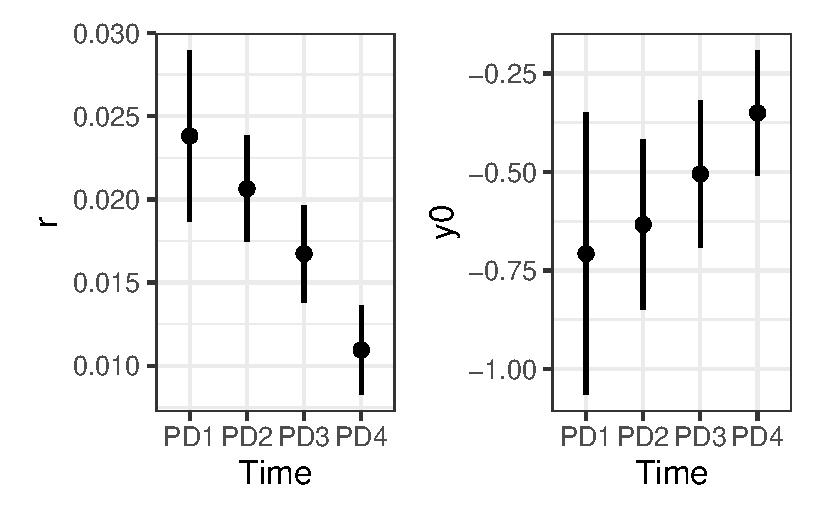
\includegraphics{./temporal-fitting_files/figure-pdf/unnamed-chunk-52-1.pdf}

}

\end{figure}

\hypertarget{simulation}{%
\chapter{Simulation}\label{simulation}}

\begin{tcolorbox}[enhanced jigsaw, rightrule=.15mm, left=2mm, breakable, colframe=quarto-callout-note-color-frame, toprule=.15mm, leftrule=.75mm, bottomrule=.15mm, colback=white, arc=.35mm, opacityback=0]
\begin{minipage}[t]{5.5mm}
\textcolor{quarto-callout-note-color}{\faInfo}
\end{minipage}%
\begin{minipage}[t]{\textwidth - 5.5mm}
This is a work in progress that is currently undergoing heavy technical
editing and copy-editing\end{minipage}%
\end{tcolorbox}

\begin{Shaded}
\begin{Highlighting}[]
\FunctionTok{library}\NormalTok{(tidyverse) }\CommentTok{\# essential packages }
\FunctionTok{library}\NormalTok{(cowplot) }\CommentTok{\# for themes }
\FunctionTok{library}\NormalTok{(deSolve)}
\FunctionTok{theme\_set}\NormalTok{(}\FunctionTok{theme\_bw}\NormalTok{(}\AttributeTok{base\_size =} \DecValTok{16}\NormalTok{)) }\CommentTok{\# set global theme}
\end{Highlighting}
\end{Shaded}

\begin{Shaded}
\begin{Highlighting}[]
\NormalTok{HLIR\_fun }\OtherTok{\textless{}{-}} \ControlFlowTok{function}\NormalTok{(t, y, par) \{}
  \CommentTok{\# Variables}
\NormalTok{  H }\OtherTok{\textless{}{-}}\NormalTok{ y[}\DecValTok{1}\NormalTok{]}
\NormalTok{  L }\OtherTok{\textless{}{-}}\NormalTok{ y[}\DecValTok{2}\NormalTok{]}
\NormalTok{  I }\OtherTok{\textless{}{-}}\NormalTok{ y[}\DecValTok{3}\NormalTok{]}
\NormalTok{  R }\OtherTok{\textless{}{-}}\NormalTok{ y[}\DecValTok{4}\NormalTok{]}
\NormalTok{  beta }\OtherTok{\textless{}{-}}\NormalTok{ par}\SpecialCharTok{$}\NormalTok{beta}
\NormalTok{  gama }\OtherTok{\textless{}{-}}\NormalTok{ par}\SpecialCharTok{$}\NormalTok{gama}
\NormalTok{  mu }\OtherTok{\textless{}{-}}\NormalTok{ par}\SpecialCharTok{$}\NormalTok{mu}

  \CommentTok{\# Right hand side of the model}
\NormalTok{  dH }\OtherTok{\textless{}{-}} \SpecialCharTok{{-}}\NormalTok{beta }\SpecialCharTok{*}\NormalTok{ H }\SpecialCharTok{*}\NormalTok{ I}
\NormalTok{  dL }\OtherTok{\textless{}{-}}\NormalTok{ beta }\SpecialCharTok{*}\NormalTok{ H }\SpecialCharTok{*}\NormalTok{ I }\SpecialCharTok{{-}}\NormalTok{ gama }\SpecialCharTok{*}\NormalTok{ L}
\NormalTok{  dI }\OtherTok{\textless{}{-}}\NormalTok{ gama }\SpecialCharTok{*}\NormalTok{ L }\SpecialCharTok{{-}}\NormalTok{ mu }\SpecialCharTok{*}\NormalTok{ I}
\NormalTok{  dR }\OtherTok{\textless{}{-}}\NormalTok{ mu }\SpecialCharTok{*}\NormalTok{ I}
  \FunctionTok{return}\NormalTok{(}\FunctionTok{list}\NormalTok{(}\FunctionTok{c}\NormalTok{(dH, dL, dI, dR)))}
\NormalTok{\}}
\end{Highlighting}
\end{Shaded}

\hypertarget{setting-up}{%
\section{Setting up}\label{setting-up}}

\begin{Shaded}
\begin{Highlighting}[]
\CommentTok{\# Set up parameters}
\NormalTok{beta }\OtherTok{\textless{}{-}} \FloatTok{0.002} \CommentTok{\# Per capita rate of infection of susceptible hosts}
\NormalTok{gama }\OtherTok{\textless{}{-}} \DecValTok{1} \SpecialCharTok{/} \DecValTok{5} \CommentTok{\#  Rate at which exposed (i.e., latently infected) hosts become infectious}
\NormalTok{delta }\OtherTok{\textless{}{-}} \DecValTok{15} \CommentTok{\# infectious period}
\NormalTok{mu }\OtherTok{\textless{}{-}} \DecValTok{1} \SpecialCharTok{/}\NormalTok{ delta}
\NormalTok{InitCond }\OtherTok{\textless{}{-}} \FunctionTok{c}\NormalTok{(}\DecValTok{1000}\NormalTok{, }\DecValTok{1}\NormalTok{, }\DecValTok{0}\NormalTok{, }\DecValTok{0}\NormalTok{)}
\end{Highlighting}
\end{Shaded}

\hypertarget{solving-equation}{%
\section{Solving equation}\label{solving-equation}}

\begin{Shaded}
\begin{Highlighting}[]
\NormalTok{steps }\OtherTok{\textless{}{-}} \FunctionTok{seq}\NormalTok{(}\DecValTok{1}\NormalTok{, }\DecValTok{60}\NormalTok{, }\AttributeTok{by =} \DecValTok{1}\NormalTok{)}
\NormalTok{parms }\OtherTok{\textless{}{-}} \FunctionTok{list}\NormalTok{(}\AttributeTok{beta =}\NormalTok{ beta, }\AttributeTok{gama =}\NormalTok{ gama, }\AttributeTok{mu =}\NormalTok{ mu)}
\NormalTok{HLIR }\OtherTok{\textless{}{-}} \FunctionTok{ode}\NormalTok{(InitCond, steps, HLIR\_fun, parms)}
\NormalTok{epidemics }\OtherTok{\textless{}{-}} \FunctionTok{data.frame}\NormalTok{(}\AttributeTok{time =}\NormalTok{ HLIR[, }\DecValTok{1}\NormalTok{], }\AttributeTok{H =}\NormalTok{ HLIR[, }\DecValTok{2}\NormalTok{], }\AttributeTok{L =}\NormalTok{ HLIR[, }\DecValTok{3}\NormalTok{], }\AttributeTok{I =}\NormalTok{ HLIR[, }\DecValTok{4}\NormalTok{], }\AttributeTok{R =}\NormalTok{ HLIR[, }\DecValTok{5}\NormalTok{])}
\end{Highlighting}
\end{Shaded}

\hypertarget{visualizing-hlir-output}{%
\section{Visualizing HLIR output}\label{visualizing-hlir-output}}

\begin{Shaded}
\begin{Highlighting}[]
\FunctionTok{library}\NormalTok{(ggthemes)}
\end{Highlighting}
\end{Shaded}

\begin{verbatim}

Attaching package: 'ggthemes'
\end{verbatim}

\begin{verbatim}
The following object is masked from 'package:cowplot':

    theme_map
\end{verbatim}

\begin{Shaded}
\begin{Highlighting}[]
\NormalTok{p1 }\OtherTok{\textless{}{-}}\NormalTok{ epidemics }\SpecialCharTok{\%\textgreater{}\%}
  \FunctionTok{ggplot}\NormalTok{() }\SpecialCharTok{+}
  \FunctionTok{geom\_line}\NormalTok{(}\FunctionTok{aes}\NormalTok{(time, H, }\AttributeTok{color =} \StringTok{"H"}\NormalTok{), }\AttributeTok{size =} \DecValTok{2}\NormalTok{) }\SpecialCharTok{+}
  \FunctionTok{geom\_line}\NormalTok{(}\FunctionTok{aes}\NormalTok{(time, L, }\AttributeTok{color =} \StringTok{"L"}\NormalTok{), }\AttributeTok{size =} \DecValTok{2}\NormalTok{) }\SpecialCharTok{+}
  \FunctionTok{geom\_line}\NormalTok{(}\FunctionTok{aes}\NormalTok{(time, I, }\AttributeTok{color =} \StringTok{"I"}\NormalTok{), }\AttributeTok{size =} \DecValTok{2}\NormalTok{) }\SpecialCharTok{+}
  \FunctionTok{geom\_line}\NormalTok{(}\FunctionTok{aes}\NormalTok{(time, R, }\AttributeTok{color =} \StringTok{"R"}\NormalTok{), }\AttributeTok{size =} \DecValTok{2}\NormalTok{) }\SpecialCharTok{+}
  \FunctionTok{geom\_line}\NormalTok{(}\FunctionTok{aes}\NormalTok{(time, I}\SpecialCharTok{+}\NormalTok{R, }\AttributeTok{color =} \StringTok{"DIS"}\NormalTok{), }\AttributeTok{size =}\DecValTok{2}\NormalTok{, }\AttributeTok{linetype =} \DecValTok{2}\NormalTok{)}\SpecialCharTok{+}
  \FunctionTok{labs}\NormalTok{(}\AttributeTok{y =} \StringTok{"Population size (count)"}\NormalTok{, }\AttributeTok{x =} \StringTok{"Time (days)"}\NormalTok{, }\AttributeTok{color =} \StringTok{"Sites"}\NormalTok{) }
\NormalTok{ p1}
\end{Highlighting}
\end{Shaded}

\begin{figure}[H]

{\centering 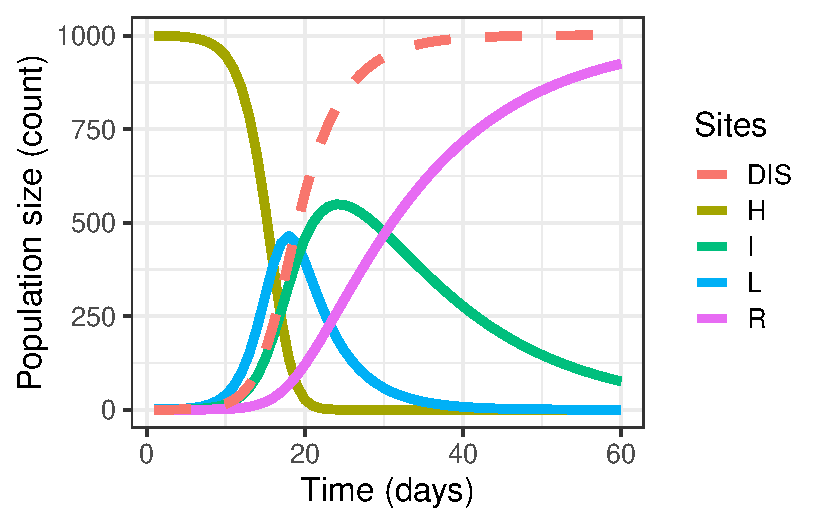
\includegraphics{./temporal-simulation_files/figure-pdf/unnamed-chunk-10-1.pdf}

}

\end{figure}

\part{Spatial analysis}

\hypertarget{spatial-gradients}{%
\chapter{Spatial gradients}\label{spatial-gradients}}

\begin{tcolorbox}[enhanced jigsaw, rightrule=.15mm, left=2mm, breakable, colframe=quarto-callout-note-color-frame, toprule=.15mm, leftrule=.75mm, bottomrule=.15mm, colback=white, arc=.35mm, opacityback=0]
\begin{minipage}[t]{5.5mm}
\textcolor{quarto-callout-note-color}{\faInfo}
\end{minipage}%
\begin{minipage}[t]{\textwidth - 5.5mm}
This is a work in progress that is currently undergoing heavy technical
editing and copy-editing\end{minipage}%
\end{tcolorbox}

\hypertarget{introduction-1}{%
\section{Introduction}\label{introduction-1}}

The assessment of disease in space, in terms of changes in the intensity
as it spreads over distance, is called \textbf{disease gradient}. In
reality, it is the dispersal (migration) of the pathogen by various
means (e.g.~wind, vectors, rain, movement of infected material or human
mediation) that promotes the spread of plant diseases within a field or
across continents and generates the disease gradients. There are two
kinds of gradients, the inoculum gradient where host availability is not
necessarily required and the disease gradient where the three elements
of the disease triangle are required. Let's see examples of actual
disease gradients measured in the field with quite distinct patterns.

In the first example (Mundt et al. 1999), the objective of the authors
was to measure the dispersal potential of the pathogenic bacteria
\emph{Xanthomonas oryzae} pv. \emph{oryzae} that causes leaf blight on
rice using experimental plots in the Philippines, during the wet seasons
of 1994 and 1995. The data were made available
\href{https://www.apsnet.org/edcenter/disimpactmngmnt/topc/EcologyAndEpidemiologyInR/ModelingDispersalGradients/Pages/PrimaryDiseaseGradientsofBacteria.aspx}{in
this tutorial}. We enter the data manually and then produce two plots,
one for each year.

\begin{Shaded}
\begin{Highlighting}[]
\FunctionTok{library}\NormalTok{(tidyverse)}
\FunctionTok{theme\_set}\NormalTok{(}\FunctionTok{theme\_bw}\NormalTok{())}
\NormalTok{d }\OtherTok{\textless{}{-}} \FunctionTok{c}\NormalTok{(}\FloatTok{0.0}\NormalTok{, }\FloatTok{0.22}\NormalTok{, }\FloatTok{0.44}\NormalTok{, }\FloatTok{0.66}\NormalTok{) }\CommentTok{\# distance in meters}
\NormalTok{y4 }\OtherTok{\textless{}{-}} \FunctionTok{c}\NormalTok{(}\FloatTok{3.083}\NormalTok{, }\FloatTok{0.521}\NormalTok{, }\FloatTok{0.083}\NormalTok{, }\FloatTok{0.021}\NormalTok{) }\CommentTok{\# n. of new lesions in 1994 trial}
\NormalTok{y5 }\OtherTok{\textless{}{-}} \FunctionTok{c}\NormalTok{(}\FloatTok{7.185}\NormalTok{, .}\DecValTok{380}\NormalTok{, }\FloatTok{0.157}\NormalTok{, }\FloatTok{0.028}\NormalTok{) }\CommentTok{\# n. of new lesion in 1995 trial}
\NormalTok{xo }\OtherTok{\textless{}{-}} \FunctionTok{data.frame}\NormalTok{(d, y4, y5)}

\NormalTok{g1 }\OtherTok{\textless{}{-}}\NormalTok{ xo }\SpecialCharTok{|\textgreater{}} 
  \FunctionTok{ggplot}\NormalTok{(}\FunctionTok{aes}\NormalTok{(d, y4))}\SpecialCharTok{+}
  \FunctionTok{geom\_point}\NormalTok{()}\SpecialCharTok{+}
  \FunctionTok{geom\_line}\NormalTok{()}\SpecialCharTok{+}
  \FunctionTok{ylim}\NormalTok{(}\DecValTok{0}\NormalTok{,}\DecValTok{8}\NormalTok{)}\SpecialCharTok{+}
  \FunctionTok{labs}\NormalTok{(}\AttributeTok{y =} \StringTok{"N. of new lesions"}\NormalTok{,}
       \AttributeTok{x =} \StringTok{"Distance (m)"}\NormalTok{,}
       \AttributeTok{title =} \StringTok{"1994 wet season"}\NormalTok{)}

\NormalTok{g2 }\OtherTok{\textless{}{-}}\NormalTok{ xo }\SpecialCharTok{|\textgreater{}} 
  \FunctionTok{ggplot}\NormalTok{(}\FunctionTok{aes}\NormalTok{(d, y5))}\SpecialCharTok{+}
  \FunctionTok{geom\_point}\NormalTok{()}\SpecialCharTok{+}
  \FunctionTok{geom\_line}\NormalTok{()}\SpecialCharTok{+}
   \FunctionTok{ylim}\NormalTok{(}\DecValTok{0}\NormalTok{,}\DecValTok{8}\NormalTok{)}\SpecialCharTok{+}
  \FunctionTok{labs}\NormalTok{(}\AttributeTok{y =} \StringTok{"N. of new lesions"}\NormalTok{,}
       \AttributeTok{x =} \StringTok{"Distance (m)"}\NormalTok{,}
       \AttributeTok{title =} \StringTok{"1995 wet season"}\NormalTok{)}

\FunctionTok{library}\NormalTok{(patchwork)}
\NormalTok{(g1 }\SpecialCharTok{|}\NormalTok{ g2) }\SpecialCharTok{+}  \FunctionTok{plot\_annotation}\NormalTok{(}
  \AttributeTok{title =} \StringTok{\textquotesingle{}Primary gradients of bacterial blight of rice\textquotesingle{}}\NormalTok{,}
  \AttributeTok{caption =} \StringTok{"Source: Mundt et al. (1999)"}\NormalTok{)}
\end{Highlighting}
\end{Shaded}

\begin{figure}[H]

{\centering 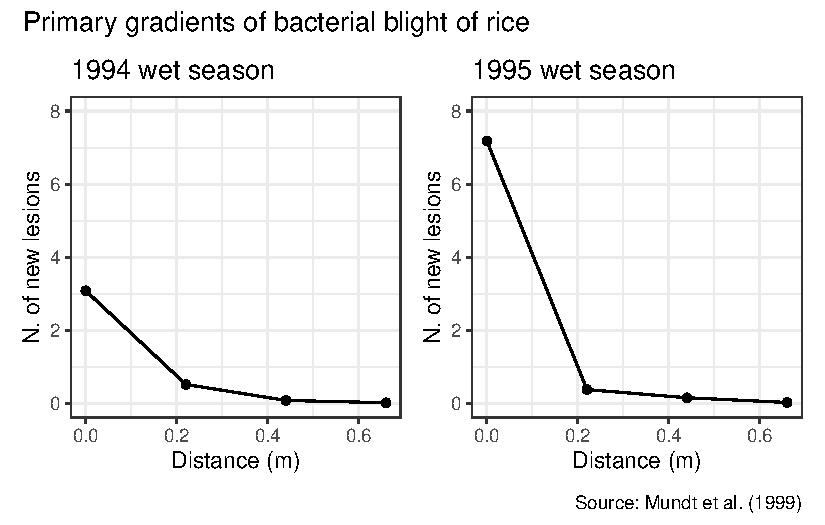
\includegraphics{./spatial-gradients_files/figure-pdf/unnamed-chunk-2-1.pdf}

}

\end{figure}

The second gradient is of stripe rust, caused by \emph{Puccinia
striiformis} f.~sp. \emph{tritici,} on wheat collected in a field
experiment at Hermiston in 2002 (Sackett and Mundt 2005) and whose data
was made freely available (Mikaberidze et al. 2015). Let's enter data
manually as a tibble format. There are five columns. The first and
second are distances in feet and meters, respectively, from the source
of infection. The other three columns are measures of stripe rust
severity on replicated plots.

\begin{Shaded}
\begin{Highlighting}[]
\NormalTok{hermiston }\OtherTok{\textless{}{-}} 
\NormalTok{  tibble}\SpecialCharTok{::}\FunctionTok{tribble}\NormalTok{(}
  \SpecialCharTok{\textasciitilde{}}\NormalTok{dist\_f, }\SpecialCharTok{\textasciitilde{}}\NormalTok{dist\_m,  }\SpecialCharTok{\textasciitilde{}}\StringTok{\textasciigrave{}}\AttributeTok{1}\StringTok{\textasciigrave{}}\NormalTok{,  }\SpecialCharTok{\textasciitilde{}}\StringTok{\textasciigrave{}}\AttributeTok{2}\StringTok{\textasciigrave{}}\NormalTok{,  }\SpecialCharTok{\textasciitilde{}}\StringTok{\textasciigrave{}}\AttributeTok{3}\StringTok{\textasciigrave{}}\NormalTok{,}
  \DecValTok{0}\NormalTok{,       }\DecValTok{0}\NormalTok{,    }\DecValTok{65}\NormalTok{,    }\DecValTok{65}\NormalTok{,    }\DecValTok{39}\NormalTok{,}
  \DecValTok{5}\NormalTok{,     }\FloatTok{1.5}\NormalTok{,    }\DecValTok{35}\NormalTok{,    }\DecValTok{44}\NormalTok{,   }\FloatTok{7.5}\NormalTok{,}
  \DecValTok{10}\NormalTok{,       }\DecValTok{3}\NormalTok{,  }\FloatTok{21.5}\NormalTok{,  }\FloatTok{14.5}\NormalTok{,  }\FloatTok{1.75}\NormalTok{,}
  \DecValTok{20}\NormalTok{,     }\FloatTok{6.1}\NormalTok{,     }\DecValTok{8}\NormalTok{,  }\FloatTok{0.75}\NormalTok{,   }\FloatTok{0.2}\NormalTok{,}
  \DecValTok{40}\NormalTok{,    }\FloatTok{12.2}\NormalTok{,     }\DecValTok{1}\NormalTok{,  }\FloatTok{0.08}\NormalTok{, }\FloatTok{0.025}\NormalTok{,}
  \DecValTok{60}\NormalTok{,    }\FloatTok{18.3}\NormalTok{,  }\FloatTok{0.25}\NormalTok{, }\FloatTok{0.026}\NormalTok{, }\FloatTok{0.015}\NormalTok{,}
  \DecValTok{80}\NormalTok{,    }\FloatTok{24.4}\NormalTok{, }\FloatTok{0.035}\NormalTok{, }\FloatTok{0.015}\NormalTok{, }\FloatTok{0.009}\NormalTok{,}
  \DecValTok{100}\NormalTok{,    }\FloatTok{30.5}\NormalTok{,  }\FloatTok{0.01}\NormalTok{, }\FloatTok{0.003}\NormalTok{, }\FloatTok{0.008}\NormalTok{,}
  \DecValTok{120}\NormalTok{,    }\FloatTok{36.6}\NormalTok{, }\FloatTok{0.008}\NormalTok{, }\FloatTok{0.016}\NormalTok{,  }\FloatTok{0.01}\NormalTok{,}
  \DecValTok{140}\NormalTok{,    }\FloatTok{42.7}\NormalTok{, }\FloatTok{0.003}\NormalTok{, }\FloatTok{0.003}\NormalTok{,  }\FloatTok{0.01}\NormalTok{,}
  \DecValTok{160}\NormalTok{,    }\FloatTok{48.8}\NormalTok{, }\FloatTok{0.001}\NormalTok{, }\FloatTok{0.006}\NormalTok{, }\FloatTok{0.006}\NormalTok{,}
  \DecValTok{180}\NormalTok{,    }\FloatTok{54.9}\NormalTok{, }\FloatTok{0.001}\NormalTok{, }\FloatTok{0.002}\NormalTok{, }\FloatTok{0.002}\NormalTok{,}
  \DecValTok{200}\NormalTok{,      }\DecValTok{61}\NormalTok{, }\FloatTok{0.001}\NormalTok{, }\FloatTok{0.003}\NormalTok{, }\FloatTok{0.004}\NormalTok{,}
  \DecValTok{220}\NormalTok{,    }\FloatTok{67.1}\NormalTok{, }\FloatTok{0.001}\NormalTok{, }\FloatTok{0.003}\NormalTok{, }\FloatTok{0.002}\NormalTok{,}
  \DecValTok{240}\NormalTok{,    }\FloatTok{73.2}\NormalTok{, }\FloatTok{0.001}\NormalTok{, }\FloatTok{0.001}\NormalTok{,     }\DecValTok{0}\NormalTok{,}
  \DecValTok{260}\NormalTok{,    }\FloatTok{79.2}\NormalTok{, }\FloatTok{0.001}\NormalTok{, }\FloatTok{0.002}\NormalTok{,     }\DecValTok{0}\NormalTok{,}
  \DecValTok{280}\NormalTok{,    }\FloatTok{85.3}\NormalTok{, }\FloatTok{0.001}\NormalTok{, }\FloatTok{0.001}\NormalTok{,     }\DecValTok{0}\NormalTok{,}
  \DecValTok{300}\NormalTok{,    }\FloatTok{91.4}\NormalTok{, }\FloatTok{0.001}\NormalTok{, }\FloatTok{0.001}\NormalTok{, }\FloatTok{0.001}
\NormalTok{  )}
\end{Highlighting}
\end{Shaded}

\begin{Shaded}
\begin{Highlighting}[]
\FunctionTok{library}\NormalTok{(tidyverse)}
\FunctionTok{library}\NormalTok{(ggthemes)}
\FunctionTok{theme\_set}\NormalTok{(}\FunctionTok{theme\_bw}\NormalTok{())}
\NormalTok{hermiston }\SpecialCharTok{|\textgreater{}} 
  \FunctionTok{pivot\_longer}\NormalTok{(}\DecValTok{3}\SpecialCharTok{:}\DecValTok{5}\NormalTok{, }\AttributeTok{names\_to =} \StringTok{"replicate"}\NormalTok{, }\AttributeTok{values\_to =} \StringTok{"severity"}\NormalTok{) }\SpecialCharTok{|\textgreater{}} 
  \FunctionTok{ggplot}\NormalTok{(}\FunctionTok{aes}\NormalTok{(dist\_m, severity, }\AttributeTok{color =}\NormalTok{ replicate))}\SpecialCharTok{+}
  \FunctionTok{geom\_point}\NormalTok{(}\AttributeTok{size =} \DecValTok{2}\NormalTok{)}\SpecialCharTok{+}
  \FunctionTok{geom\_line}\NormalTok{(}\AttributeTok{size =} \DecValTok{1}\NormalTok{)}\SpecialCharTok{+}
  \FunctionTok{scale\_color\_colorblind}\NormalTok{()}\SpecialCharTok{+}
  \FunctionTok{labs}\NormalTok{(}\AttributeTok{title =} \StringTok{"Primary disease gradients"}\NormalTok{, }
       \AttributeTok{x =} \StringTok{"Distance from the source (m)"}\NormalTok{,}
       \AttributeTok{y =} \StringTok{"Stripe rust severity (\%)"}\NormalTok{,}
       \AttributeTok{color =} \StringTok{"Replicate"}\NormalTok{,}
       \AttributeTok{caption =} \StringTok{"source: Sackett et al. (2005)"}\NormalTok{)}
\end{Highlighting}
\end{Shaded}

\begin{figure}[H]

{\centering 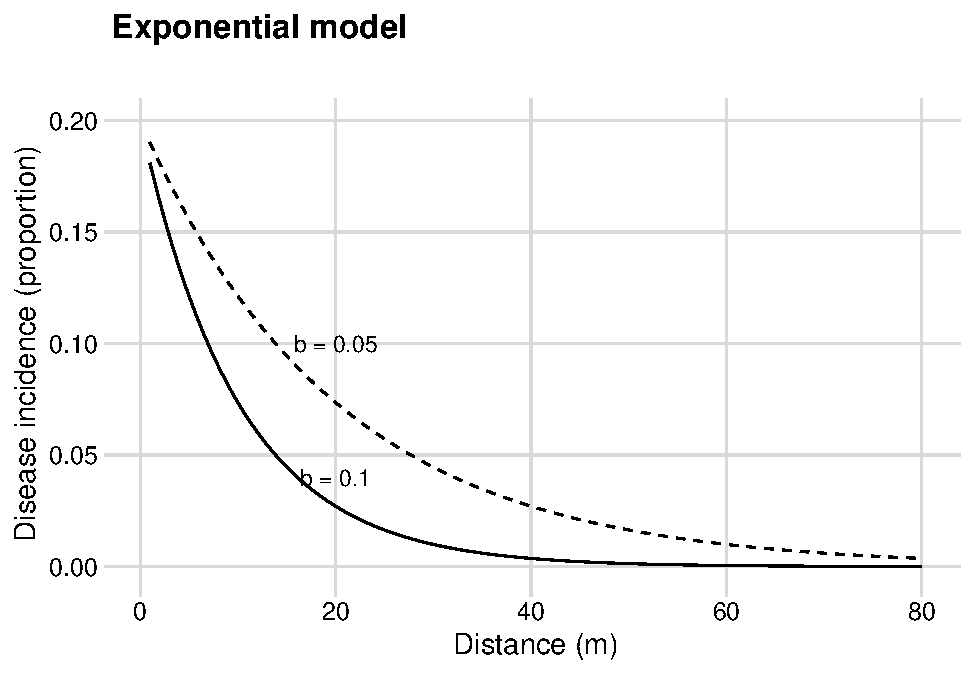
\includegraphics{./spatial-gradients_files/figure-pdf/unnamed-chunk-6-1.pdf}

}

\end{figure}

As it is clear in the above examples, in disease gradients, assuming
that there is only a single source of inoculum, the intensity of the
disease decreases more steeply within short distances of the source, and
less steeply at greater distances until they reach zero or a low
background level of occasional diseased plants.

The shapes of the gradients are defined by mechanisms associated with
the dispersal of the inoculum which depends on the biology of the
pathogen but strongly to environmental factors that affect pathogen
dispersal.

When studying disease gradients, researchers need to make sure that
there is a well-defined single source of inoculum. In gradients, this is
called a \textbf{focus} (where foci are deemed the plural), from where
the inoculum originates. Three types of foci can be defined: point, line
or area sources. While the point source can be a plant or group of
plants at any position in the plot or field (center or corner), line and
area sources are usually defined as one or more rows of diseased plants
at one side of the plot or field.

\begin{Shaded}
\begin{Highlighting}[]
\FunctionTok{library}\NormalTok{(ggplot2)}
\FunctionTok{library}\NormalTok{(gganimate)}
\NormalTok{line }\OtherTok{\textless{}{-}} \FunctionTok{ggplot}\NormalTok{(}\FunctionTok{data.frame}\NormalTok{(}\FunctionTok{c}\NormalTok{(}\DecValTok{1}\SpecialCharTok{:}\DecValTok{10}\NormalTok{),}\FunctionTok{c}\NormalTok{(}\DecValTok{1}\SpecialCharTok{:}\DecValTok{10}\NormalTok{)))}\SpecialCharTok{+}
  \FunctionTok{annotate}\NormalTok{(}\StringTok{"rect"}\NormalTok{, }\AttributeTok{xmin =} \DecValTok{0}\NormalTok{, }\AttributeTok{xmax =} \DecValTok{10}\NormalTok{, }\AttributeTok{ymin =} \DecValTok{0}\NormalTok{, }\AttributeTok{ymax =} \DecValTok{10}\NormalTok{, }\AttributeTok{fill =} \StringTok{"gray92"}\NormalTok{)}\SpecialCharTok{+}
  \FunctionTok{annotate}\NormalTok{(}\StringTok{"rect"}\NormalTok{, }\AttributeTok{xmin =} \DecValTok{0}\NormalTok{, }\AttributeTok{xmax =} \DecValTok{10}\NormalTok{, }\AttributeTok{ymin =} \FloatTok{9.7}\NormalTok{, }\AttributeTok{ymax =} \DecValTok{10}\NormalTok{, }\AttributeTok{color =} \StringTok{"black"}\NormalTok{, }\AttributeTok{fill =} \StringTok{"orange"}\NormalTok{)}\SpecialCharTok{+}
  \FunctionTok{annotate}\NormalTok{(}\StringTok{"segment"}\NormalTok{, }\AttributeTok{size =} \DecValTok{2}\NormalTok{, }\AttributeTok{x =} \DecValTok{1}\NormalTok{, }\AttributeTok{xend =} \DecValTok{1}\NormalTok{, }\AttributeTok{y =} \FloatTok{9.5}\NormalTok{, }\AttributeTok{yend =} \DecValTok{2}\NormalTok{, }\AttributeTok{arrow =} \FunctionTok{arrow}\NormalTok{())}\SpecialCharTok{+}
  \FunctionTok{annotate}\NormalTok{(}\StringTok{"segment"}\NormalTok{, }\AttributeTok{size =} \DecValTok{2}\NormalTok{, }\AttributeTok{x =} \DecValTok{3}\NormalTok{, }\AttributeTok{xend =} \DecValTok{3}\NormalTok{, }\AttributeTok{y =} \FloatTok{9.5}\NormalTok{, }\AttributeTok{yend =} \DecValTok{2}\NormalTok{, }\AttributeTok{arrow =} \FunctionTok{arrow}\NormalTok{())}\SpecialCharTok{+}
  \FunctionTok{annotate}\NormalTok{(}\StringTok{"segment"}\NormalTok{, }\AttributeTok{size =} \DecValTok{2}\NormalTok{, }\AttributeTok{x =} \DecValTok{5}\NormalTok{, }\AttributeTok{xend =} \DecValTok{5}\NormalTok{, }\AttributeTok{y =} \FloatTok{9.5}\NormalTok{, }\AttributeTok{yend =} \DecValTok{2}\NormalTok{, }\AttributeTok{arrow =} \FunctionTok{arrow}\NormalTok{())}\SpecialCharTok{+}
  \FunctionTok{annotate}\NormalTok{(}\StringTok{"segment"}\NormalTok{, }\AttributeTok{size =} \DecValTok{2}\NormalTok{, }\AttributeTok{x =} \DecValTok{7}\NormalTok{, }\AttributeTok{xend =} \DecValTok{7}\NormalTok{, }\AttributeTok{y =} \FloatTok{9.5}\NormalTok{, }\AttributeTok{yend =} \DecValTok{2}\NormalTok{, }\AttributeTok{arrow =} \FunctionTok{arrow}\NormalTok{())}\SpecialCharTok{+}
  \FunctionTok{annotate}\NormalTok{(}\StringTok{"segment"}\NormalTok{, }\AttributeTok{size =} \DecValTok{2}\NormalTok{, }\AttributeTok{x =} \DecValTok{9}\NormalTok{, }\AttributeTok{xend =} \DecValTok{9}\NormalTok{, }\AttributeTok{y =} \FloatTok{9.5}\NormalTok{, }\AttributeTok{yend =} \DecValTok{2}\NormalTok{, }\AttributeTok{arrow =} \FunctionTok{arrow}\NormalTok{())}\SpecialCharTok{+}
  \FunctionTok{ylim}\NormalTok{(}\DecValTok{0}\NormalTok{,}\DecValTok{10}\NormalTok{)}\SpecialCharTok{+}
  \FunctionTok{xlim}\NormalTok{(}\DecValTok{0}\NormalTok{,}\DecValTok{10}\NormalTok{)}\SpecialCharTok{+}
  \FunctionTok{coord\_fixed}\NormalTok{()}\SpecialCharTok{+}
  \FunctionTok{theme\_void}\NormalTok{()}\SpecialCharTok{+}
  \FunctionTok{labs}\NormalTok{(}\AttributeTok{title =} \StringTok{"      Side line"}\NormalTok{)}

\NormalTok{area }\OtherTok{\textless{}{-}} \FunctionTok{ggplot}\NormalTok{(}\FunctionTok{data.frame}\NormalTok{(}\FunctionTok{c}\NormalTok{(}\DecValTok{1}\SpecialCharTok{:}\DecValTok{10}\NormalTok{),}\FunctionTok{c}\NormalTok{(}\DecValTok{1}\SpecialCharTok{:}\DecValTok{10}\NormalTok{)))}\SpecialCharTok{+}
  \FunctionTok{annotate}\NormalTok{(}\StringTok{"rect"}\NormalTok{, }\AttributeTok{xmin =} \DecValTok{0}\NormalTok{, }\AttributeTok{xmax =} \DecValTok{10}\NormalTok{, }\AttributeTok{ymin =} \DecValTok{0}\NormalTok{, }\AttributeTok{ymax =} \DecValTok{10}\NormalTok{, }\AttributeTok{fill =} \StringTok{"gray92"}\NormalTok{)}\SpecialCharTok{+}
  \FunctionTok{annotate}\NormalTok{(}\StringTok{"rect"}\NormalTok{, }\AttributeTok{xmin =} \DecValTok{0}\NormalTok{, }\AttributeTok{xmax =} \DecValTok{10}\NormalTok{, }\AttributeTok{ymin =} \FloatTok{8.2}\NormalTok{, }\AttributeTok{ymax =} \DecValTok{10}\NormalTok{, }\AttributeTok{color =} \StringTok{"black"}\NormalTok{, }\AttributeTok{fill =} \StringTok{"orange"}\NormalTok{)}\SpecialCharTok{+}
  \FunctionTok{annotate}\NormalTok{(}\StringTok{"segment"}\NormalTok{, }\AttributeTok{size =} \DecValTok{2}\NormalTok{, }\AttributeTok{x =} \DecValTok{1}\NormalTok{, }\AttributeTok{xend =} \DecValTok{1}\NormalTok{, }\AttributeTok{y =} \DecValTok{8}\NormalTok{, }\AttributeTok{yend =} \DecValTok{2}\NormalTok{, }\AttributeTok{arrow =} \FunctionTok{arrow}\NormalTok{())}\SpecialCharTok{+}
  \FunctionTok{annotate}\NormalTok{(}\StringTok{"segment"}\NormalTok{, }\AttributeTok{size =} \DecValTok{2}\NormalTok{, }\AttributeTok{x =} \DecValTok{3}\NormalTok{, }\AttributeTok{xend =} \DecValTok{3}\NormalTok{, }\AttributeTok{y =} \DecValTok{8}\NormalTok{, }\AttributeTok{yend =} \DecValTok{2}\NormalTok{, }\AttributeTok{arrow =} \FunctionTok{arrow}\NormalTok{())}\SpecialCharTok{+}
  \FunctionTok{annotate}\NormalTok{(}\StringTok{"segment"}\NormalTok{, }\AttributeTok{size =} \DecValTok{2}\NormalTok{, }\AttributeTok{x =} \DecValTok{5}\NormalTok{, }\AttributeTok{xend =} \DecValTok{5}\NormalTok{, }\AttributeTok{y =} \DecValTok{8}\NormalTok{, }\AttributeTok{yend =} \DecValTok{2}\NormalTok{, }\AttributeTok{arrow =} \FunctionTok{arrow}\NormalTok{())}\SpecialCharTok{+}
  \FunctionTok{annotate}\NormalTok{(}\StringTok{"segment"}\NormalTok{, }\AttributeTok{size =} \DecValTok{2}\NormalTok{, }\AttributeTok{x =} \DecValTok{7}\NormalTok{, }\AttributeTok{xend =} \DecValTok{7}\NormalTok{, }\AttributeTok{y =} \DecValTok{8}\NormalTok{, }\AttributeTok{yend =} \DecValTok{2}\NormalTok{, }\AttributeTok{arrow =} \FunctionTok{arrow}\NormalTok{())}\SpecialCharTok{+}
  \FunctionTok{annotate}\NormalTok{(}\StringTok{"segment"}\NormalTok{, }\AttributeTok{size =} \DecValTok{2}\NormalTok{, }\AttributeTok{x =} \DecValTok{9}\NormalTok{, }\AttributeTok{xend =} \DecValTok{9}\NormalTok{, }\AttributeTok{y =} \DecValTok{8}\NormalTok{, }\AttributeTok{yend =} \DecValTok{2}\NormalTok{, }\AttributeTok{arrow =} \FunctionTok{arrow}\NormalTok{())}\SpecialCharTok{+}
  \FunctionTok{ylim}\NormalTok{(}\DecValTok{0}\NormalTok{,}\DecValTok{10}\NormalTok{)}\SpecialCharTok{+}
  \FunctionTok{xlim}\NormalTok{(}\DecValTok{0}\NormalTok{,}\DecValTok{10}\NormalTok{)}\SpecialCharTok{+}
  \FunctionTok{coord\_fixed}\NormalTok{()}\SpecialCharTok{+}
  \FunctionTok{theme\_void}\NormalTok{()}\SpecialCharTok{+}
  \FunctionTok{labs}\NormalTok{(}\AttributeTok{title =} \StringTok{"      Side area"}\NormalTok{)}

\NormalTok{point\_central }\OtherTok{\textless{}{-}} \FunctionTok{ggplot}\NormalTok{(}\FunctionTok{data.frame}\NormalTok{(}\FunctionTok{c}\NormalTok{(}\DecValTok{1}\SpecialCharTok{:}\DecValTok{10}\NormalTok{),}\FunctionTok{c}\NormalTok{(}\DecValTok{1}\SpecialCharTok{:}\DecValTok{10}\NormalTok{)))}\SpecialCharTok{+}
  \FunctionTok{annotate}\NormalTok{(}\StringTok{"rect"}\NormalTok{, }\AttributeTok{xmin =} \DecValTok{0}\NormalTok{, }\AttributeTok{xmax =} \DecValTok{10}\NormalTok{, }\AttributeTok{ymin =} \DecValTok{0}\NormalTok{, }\AttributeTok{ymax =} \DecValTok{10}\NormalTok{, }\AttributeTok{fill =} \StringTok{"gray92"}\NormalTok{)}\SpecialCharTok{+}
  \FunctionTok{annotate}\NormalTok{(}\StringTok{"segment"}\NormalTok{, }\AttributeTok{size =} \DecValTok{2}\NormalTok{, }\AttributeTok{x =} \DecValTok{5}\NormalTok{, }\AttributeTok{xend =} \DecValTok{10}\NormalTok{, }\AttributeTok{y =} \DecValTok{5}\NormalTok{, }\AttributeTok{yend =} \DecValTok{10}\NormalTok{, }\AttributeTok{arrow =} \FunctionTok{arrow}\NormalTok{())}\SpecialCharTok{+}
  \FunctionTok{annotate}\NormalTok{(}\StringTok{"segment"}\NormalTok{, }\AttributeTok{size =} \DecValTok{2}\NormalTok{, }\AttributeTok{x =} \DecValTok{5}\NormalTok{, }\AttributeTok{xend =} \DecValTok{10}\NormalTok{, }\AttributeTok{y =} \DecValTok{5}\NormalTok{, }\AttributeTok{yend =} \DecValTok{5}\NormalTok{, }\AttributeTok{arrow =} \FunctionTok{arrow}\NormalTok{())}\SpecialCharTok{+}
  \FunctionTok{annotate}\NormalTok{(}\StringTok{"segment"}\NormalTok{, }\AttributeTok{size =} \DecValTok{2}\NormalTok{, }\AttributeTok{x =} \DecValTok{5}\NormalTok{, }\AttributeTok{xend =} \DecValTok{10}\NormalTok{, }\AttributeTok{y =} \DecValTok{5}\NormalTok{, }\AttributeTok{yend =} \DecValTok{0}\NormalTok{, }\AttributeTok{arrow =} \FunctionTok{arrow}\NormalTok{())}\SpecialCharTok{+}
  \FunctionTok{annotate}\NormalTok{(}\StringTok{"segment"}\NormalTok{, }\AttributeTok{size =} \DecValTok{2}\NormalTok{, }\AttributeTok{x =} \DecValTok{5}\NormalTok{, }\AttributeTok{xend =} \DecValTok{0}\NormalTok{, }\AttributeTok{y =} \DecValTok{5}\NormalTok{, }\AttributeTok{yend =} \DecValTok{0}\NormalTok{, }\AttributeTok{arrow =} \FunctionTok{arrow}\NormalTok{())}\SpecialCharTok{+}
  \FunctionTok{annotate}\NormalTok{(}\StringTok{"segment"}\NormalTok{, }\AttributeTok{size =} \DecValTok{2}\NormalTok{, }\AttributeTok{x =} \DecValTok{5}\NormalTok{, }\AttributeTok{xend =} \DecValTok{0}\NormalTok{, }\AttributeTok{y =} \DecValTok{5}\NormalTok{, }\AttributeTok{yend =} \DecValTok{5}\NormalTok{, }\AttributeTok{arrow =} \FunctionTok{arrow}\NormalTok{())}\SpecialCharTok{+}
  \FunctionTok{annotate}\NormalTok{(}\StringTok{"segment"}\NormalTok{, }\AttributeTok{size =} \DecValTok{2}\NormalTok{, }\AttributeTok{x =} \DecValTok{5}\NormalTok{, }\AttributeTok{xend =} \DecValTok{0}\NormalTok{, }\AttributeTok{y =} \DecValTok{5}\NormalTok{, }\AttributeTok{yend =} \DecValTok{10}\NormalTok{, }\AttributeTok{arrow =} \FunctionTok{arrow}\NormalTok{())}\SpecialCharTok{+}
  \FunctionTok{annotate}\NormalTok{(}\StringTok{"segment"}\NormalTok{, }\AttributeTok{size =} \DecValTok{2}\NormalTok{, }\AttributeTok{x =} \DecValTok{5}\NormalTok{, }\AttributeTok{xend =} \DecValTok{5}\NormalTok{, }\AttributeTok{y =} \DecValTok{5}\NormalTok{, }\AttributeTok{yend =} \DecValTok{10}\NormalTok{, }\AttributeTok{arrow =} \FunctionTok{arrow}\NormalTok{())}\SpecialCharTok{+}
  \FunctionTok{annotate}\NormalTok{(}\StringTok{"segment"}\NormalTok{, }\AttributeTok{size =} \DecValTok{2}\NormalTok{, }\AttributeTok{x =} \DecValTok{5}\NormalTok{, }\AttributeTok{xend =} \DecValTok{5}\NormalTok{, }\AttributeTok{y =} \DecValTok{5}\NormalTok{, }\AttributeTok{yend =} \DecValTok{0}\NormalTok{, }\AttributeTok{arrow =} \FunctionTok{arrow}\NormalTok{())}\SpecialCharTok{+}
   \FunctionTok{annotate}\NormalTok{(}\StringTok{"rect"}\NormalTok{, }\AttributeTok{xmin =} \FloatTok{5.5}\NormalTok{, }\AttributeTok{xmax =} \FloatTok{4.5}\NormalTok{, }\AttributeTok{ymin =} \FloatTok{4.5}\NormalTok{, }\AttributeTok{ymax =} \FloatTok{5.5}\NormalTok{, }\AttributeTok{color =} \StringTok{"black"}\NormalTok{, }\AttributeTok{fill =} \StringTok{"orange"}\NormalTok{ )}\SpecialCharTok{+}
  \FunctionTok{ylim}\NormalTok{(}\DecValTok{0}\NormalTok{,}\DecValTok{10}\NormalTok{)}\SpecialCharTok{+}
  \FunctionTok{xlim}\NormalTok{(}\DecValTok{0}\NormalTok{,}\DecValTok{10}\NormalTok{)}\SpecialCharTok{+}
  \FunctionTok{coord\_fixed}\NormalTok{()}\SpecialCharTok{+}
  \FunctionTok{theme\_void}\NormalTok{()}\SpecialCharTok{+}
  \FunctionTok{labs}\NormalTok{(}\AttributeTok{title =} \StringTok{"    Central point/area"}\NormalTok{)}

\NormalTok{point\_corner }\OtherTok{\textless{}{-}} \FunctionTok{ggplot}\NormalTok{(}\FunctionTok{data.frame}\NormalTok{(}\FunctionTok{c}\NormalTok{(}\DecValTok{1}\SpecialCharTok{:}\DecValTok{10}\NormalTok{),}\FunctionTok{c}\NormalTok{(}\DecValTok{1}\SpecialCharTok{:}\DecValTok{10}\NormalTok{)))}\SpecialCharTok{+}
  \FunctionTok{annotate}\NormalTok{(}\StringTok{"rect"}\NormalTok{, }\AttributeTok{xmin =} \DecValTok{0}\NormalTok{, }\AttributeTok{xmax =} \DecValTok{10}\NormalTok{, }\AttributeTok{ymin =} \DecValTok{0}\NormalTok{, }\AttributeTok{ymax =} \DecValTok{10}\NormalTok{, }\AttributeTok{fill =} \StringTok{"gray92"}\NormalTok{)}\SpecialCharTok{+}
  \FunctionTok{annotate}\NormalTok{(}\StringTok{"segment"}\NormalTok{, }\AttributeTok{size =} \DecValTok{2}\NormalTok{, }\AttributeTok{x =} \DecValTok{0}\NormalTok{, }\AttributeTok{xend =} \DecValTok{10}\NormalTok{, }\AttributeTok{y =} \DecValTok{10}\NormalTok{, }\AttributeTok{yend =} \DecValTok{0}\NormalTok{, }\AttributeTok{arrow =} \FunctionTok{arrow}\NormalTok{())}\SpecialCharTok{+}
  \FunctionTok{annotate}\NormalTok{(}\StringTok{"segment"}\NormalTok{, }\AttributeTok{size =} \DecValTok{2}\NormalTok{, }\AttributeTok{x =} \DecValTok{0}\NormalTok{, }\AttributeTok{xend =} \FloatTok{6.6}\NormalTok{, }\AttributeTok{y =} \DecValTok{10}\NormalTok{, }\AttributeTok{yend =} \DecValTok{0}\NormalTok{, }\AttributeTok{arrow =} \FunctionTok{arrow}\NormalTok{())}\SpecialCharTok{+}
  \FunctionTok{annotate}\NormalTok{(}\StringTok{"segment"}\NormalTok{, }\AttributeTok{size =} \DecValTok{2}\NormalTok{, }\AttributeTok{x =} \DecValTok{0}\NormalTok{, }\AttributeTok{xend =} \FloatTok{3.3}\NormalTok{, }\AttributeTok{y =} \DecValTok{10}\NormalTok{, }\AttributeTok{yend =} \DecValTok{0}\NormalTok{, }\AttributeTok{arrow =} \FunctionTok{arrow}\NormalTok{())}\SpecialCharTok{+}
  \FunctionTok{annotate}\NormalTok{(}\StringTok{"segment"}\NormalTok{, }\AttributeTok{size =} \DecValTok{2}\NormalTok{, }\AttributeTok{x =} \DecValTok{0}\NormalTok{, }\AttributeTok{xend =} \DecValTok{0}\NormalTok{, }\AttributeTok{y =} \DecValTok{10}\NormalTok{, }\AttributeTok{yend =} \DecValTok{0}\NormalTok{, }\AttributeTok{arrow =} \FunctionTok{arrow}\NormalTok{())}\SpecialCharTok{+}
  \FunctionTok{annotate}\NormalTok{(}\StringTok{"segment"}\NormalTok{, }\AttributeTok{size =} \DecValTok{2}\NormalTok{, }\AttributeTok{x =} \DecValTok{0}\NormalTok{, }\AttributeTok{xend =} \DecValTok{10}\NormalTok{, }\AttributeTok{y =} \DecValTok{10}\NormalTok{, }\AttributeTok{yend =} \FloatTok{3.3}\NormalTok{, }\AttributeTok{arrow =} \FunctionTok{arrow}\NormalTok{())}\SpecialCharTok{+}
  \FunctionTok{annotate}\NormalTok{(}\StringTok{"segment"}\NormalTok{, }\AttributeTok{size =} \DecValTok{2}\NormalTok{, }\AttributeTok{x =} \DecValTok{0}\NormalTok{, }\AttributeTok{xend =} \DecValTok{10}\NormalTok{, }\AttributeTok{y =} \DecValTok{10}\NormalTok{, }\AttributeTok{yend =} \FloatTok{6.6}\NormalTok{, }\AttributeTok{arrow =} \FunctionTok{arrow}\NormalTok{())}\SpecialCharTok{+}
  \FunctionTok{annotate}\NormalTok{(}\StringTok{"segment"}\NormalTok{, }\AttributeTok{size =} \DecValTok{2}\NormalTok{, }\AttributeTok{x =} \DecValTok{0}\NormalTok{, }\AttributeTok{xend =} \DecValTok{10}\NormalTok{, }\AttributeTok{y =} \DecValTok{10}\NormalTok{, }\AttributeTok{yend =} \DecValTok{10}\NormalTok{, }\AttributeTok{arrow =} \FunctionTok{arrow}\NormalTok{())}\SpecialCharTok{+}
  \FunctionTok{annotate}\NormalTok{(}\StringTok{"rect"}\NormalTok{, }\AttributeTok{xmin =} \DecValTok{0}\NormalTok{, }\AttributeTok{xmax =} \DecValTok{1}\NormalTok{, }\AttributeTok{ymin =} \DecValTok{9}\NormalTok{, }\AttributeTok{ymax =} \DecValTok{10}\NormalTok{, }\AttributeTok{color =} \StringTok{"black"}\NormalTok{, }\AttributeTok{fill =} \StringTok{"orange"}\NormalTok{)}\SpecialCharTok{+}
  \FunctionTok{ylim}\NormalTok{(}\DecValTok{0}\NormalTok{,}\DecValTok{10}\NormalTok{)}\SpecialCharTok{+}
  \FunctionTok{xlim}\NormalTok{(}\DecValTok{0}\NormalTok{,}\DecValTok{10}\NormalTok{)}\SpecialCharTok{+}
  \FunctionTok{coord\_fixed}\NormalTok{()}\SpecialCharTok{+}
  \FunctionTok{theme\_void}\NormalTok{()}\SpecialCharTok{+}
  \FunctionTok{labs}\NormalTok{(}\AttributeTok{title =} \StringTok{"    Corner point/area"}\NormalTok{)}

\FunctionTok{library}\NormalTok{(patchwork)}
\NormalTok{p\_gradients }\OtherTok{\textless{}{-}}\NormalTok{ (line }\SpecialCharTok{|}\NormalTok{ area)}\SpecialCharTok{/}
\NormalTok{(point\_central }\SpecialCharTok{|}\NormalTok{ point\_corner)}

\FunctionTok{ggsave}\NormalTok{(}\StringTok{"imgs/gradients.png"}\NormalTok{, }\AttributeTok{width =}\DecValTok{9}\NormalTok{, }\AttributeTok{height =}\DecValTok{9}\NormalTok{, }\AttributeTok{bg =} \StringTok{"white"}\NormalTok{)}
\end{Highlighting}
\end{Shaded}

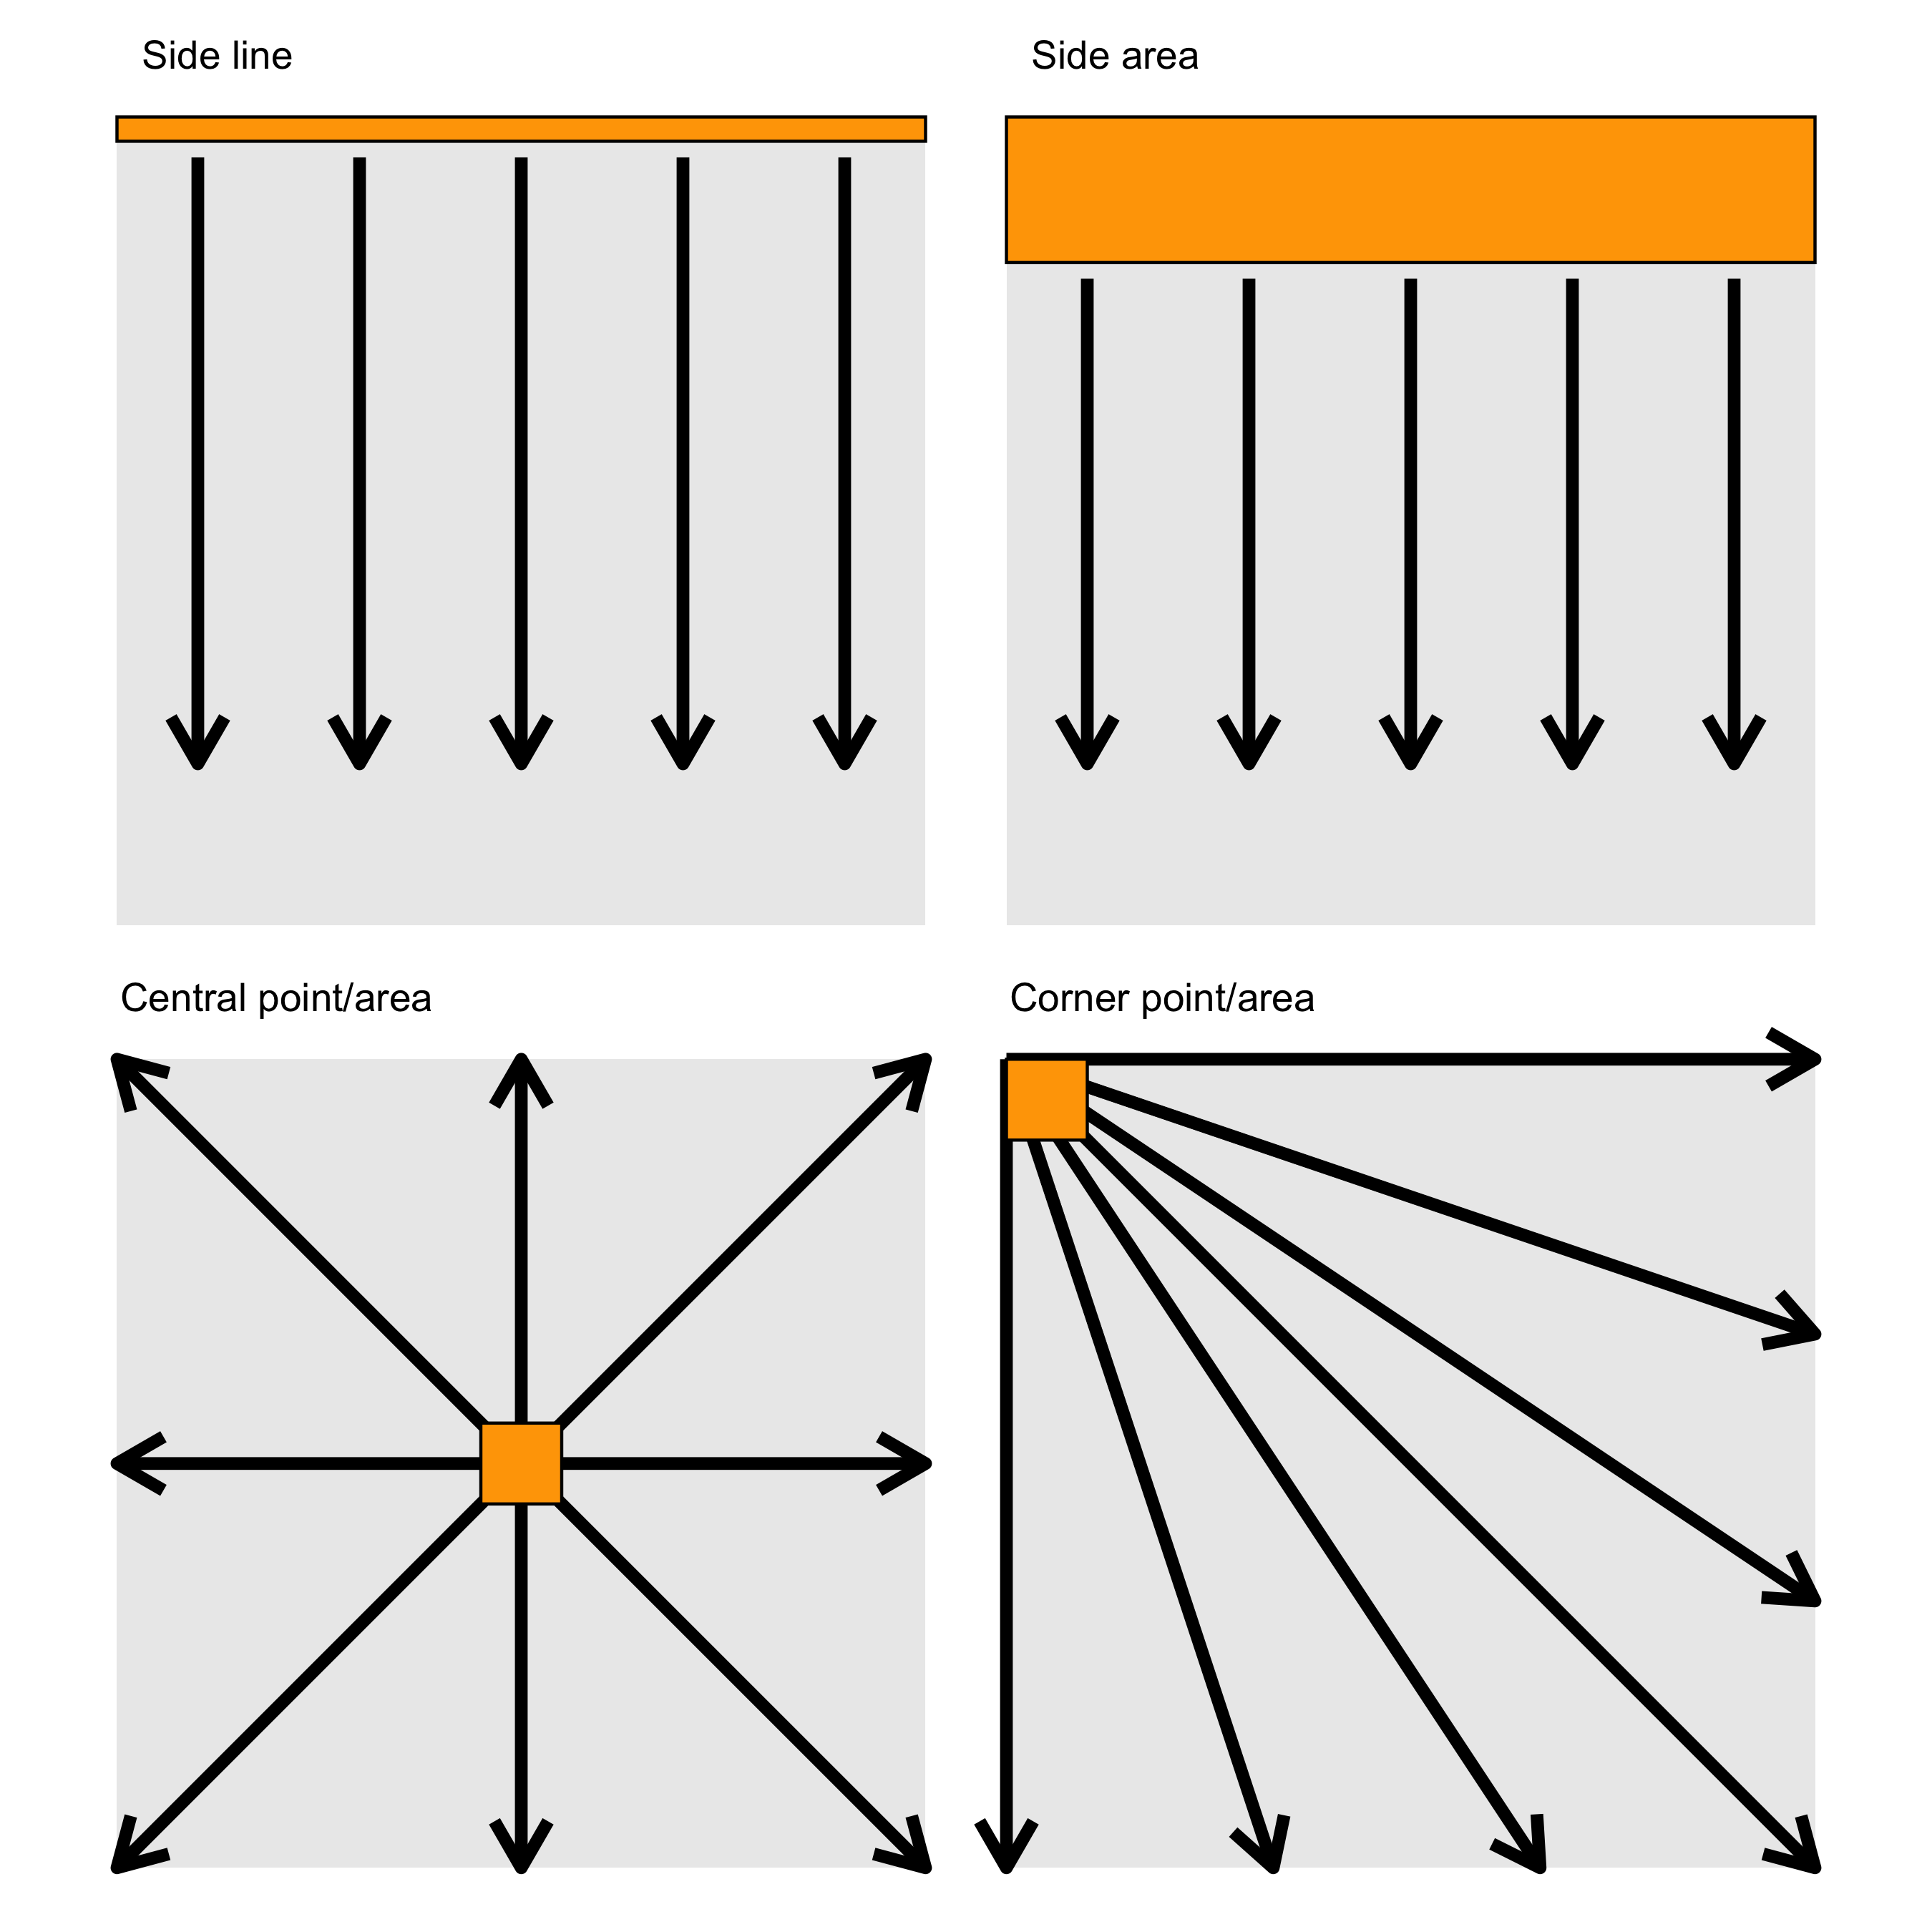
\includegraphics[width=6.08333in,height=\textheight]{./imgs/gradients.png}

The resulting gradients can be classified in two types: primary or
secondary. The primary gradient originates only from the initial focus,
while the secondary gradient originates from the movement of inoculum
produced at previously infected (due to primary gradients) plants to
other plants at increasing distances from the source. It is expected
that a mix of both kinds of gradients exists as the disease increases
over time.

As an example of primary and secondary gradients, let's visualize the
gradients of Septoria leaf spot, caused by \emph{Septoria lycopersici},
on tomato (Parker et al. 1997). The gradients were measured during two
times, thus enabling a comparison of primary and secondary
dispersal/disease gradients. More details of the study and experimental
approach were provided in
\href{https://www.apsnet.org/edcenter/disimpactmngmnt/topc/EcologyAndEpidemiologyInR/ModelingDispersalGradients/Pages/PrimaryandSecondaryGradients.aspx}{this
tutorial.} The data is entered below as a tribble and the plot produced
using g\emph{gplot2}.

\begin{Shaded}
\begin{Highlighting}[]
\NormalTok{septoria }\OtherTok{\textless{}{-}} 
\NormalTok{tibble}\SpecialCharTok{::}\FunctionTok{tribble}\NormalTok{(}
 \SpecialCharTok{\textasciitilde{}}\NormalTok{d, }\SpecialCharTok{\textasciitilde{}}\NormalTok{date1, }\SpecialCharTok{\textasciitilde{}}\NormalTok{date4,}
 \DecValTok{60}\NormalTok{,    }\DecValTok{75}\NormalTok{,    }\DecValTok{87}\NormalTok{,}
 \DecValTok{120}\NormalTok{,    }\DecValTok{40}\NormalTok{,    }\DecValTok{78}\NormalTok{,}
 \DecValTok{180}\NormalTok{,    }\DecValTok{30}\NormalTok{,    }\DecValTok{68}\NormalTok{,}
 \DecValTok{240}\NormalTok{,    }\DecValTok{20}\NormalTok{,    }\DecValTok{62}\NormalTok{,}
 \DecValTok{300}\NormalTok{,    }\DecValTok{15}\NormalTok{,    }\DecValTok{50}\NormalTok{,}
 \DecValTok{360}\NormalTok{,    }\DecValTok{12}\NormalTok{,    }\DecValTok{27}\NormalTok{,}
 \DecValTok{420}\NormalTok{,    }\DecValTok{10}\NormalTok{,    }\DecValTok{32}\NormalTok{,}
 \DecValTok{480}\NormalTok{,    }\DecValTok{12}\NormalTok{,    }\DecValTok{12}\NormalTok{,}
 \DecValTok{540}\NormalTok{,     }\DecValTok{8}\NormalTok{,    }\DecValTok{13}\NormalTok{,}
 \DecValTok{600}\NormalTok{,     }\DecValTok{5}\NormalTok{,     }\DecValTok{5}\NormalTok{,}
 \DecValTok{660}\NormalTok{,     }\DecValTok{4}\NormalTok{,     }\DecValTok{4}
\NormalTok{              )}

\NormalTok{septoria }\SpecialCharTok{|\textgreater{}} 
  \FunctionTok{pivot\_longer}\NormalTok{(}\DecValTok{2}\SpecialCharTok{:}\DecValTok{3}\NormalTok{, }\AttributeTok{names\_to =} \StringTok{"date"}\NormalTok{, }
               \AttributeTok{values\_to =} \StringTok{"defoliation"}\NormalTok{) }\SpecialCharTok{|\textgreater{}} 
  \FunctionTok{ggplot}\NormalTok{(}\FunctionTok{aes}\NormalTok{(d, defoliation, }\AttributeTok{color =}\NormalTok{ date))}\SpecialCharTok{+}
  \FunctionTok{geom\_point}\NormalTok{()}\SpecialCharTok{+}
  \FunctionTok{geom\_line}\NormalTok{()}\SpecialCharTok{+}
  \FunctionTok{scale\_color\_colorblind}\NormalTok{()}\SpecialCharTok{+}
  \FunctionTok{annotate}\NormalTok{(}\AttributeTok{geom =} \StringTok{"text"}\NormalTok{, }\AttributeTok{x =} \DecValTok{200}\NormalTok{, }\AttributeTok{y =} \DecValTok{12}\NormalTok{, }
           \AttributeTok{label =} \StringTok{"Primary gradient"}\NormalTok{, }\AttributeTok{hjust =} \StringTok{"left"}\NormalTok{)}\SpecialCharTok{+}
   \FunctionTok{annotate}\NormalTok{(}\AttributeTok{geom =} \StringTok{"text"}\NormalTok{, }\AttributeTok{x =} \DecValTok{200}\NormalTok{, }\AttributeTok{y =} \DecValTok{72}\NormalTok{, }
           \AttributeTok{label =} \StringTok{"Secondary gradient"}\NormalTok{, }\AttributeTok{hjust =} \StringTok{"left"}\NormalTok{)}\SpecialCharTok{+}
  \FunctionTok{labs}\NormalTok{(}\AttributeTok{title =} \StringTok{"Disease gradients"}\NormalTok{,}
       \AttributeTok{subtitle =} \StringTok{"Septoria leaf spot on tomato"}\NormalTok{,}
       \AttributeTok{x =} \StringTok{"Distrance from focus (m)"}\NormalTok{,}
       \AttributeTok{y =} \StringTok{"Percent defoliation"}\NormalTok{,}
       \AttributeTok{color =} \StringTok{"Date"}\NormalTok{,}
       \AttributeTok{caption =} \StringTok{"Parker et al. (1997)"}\NormalTok{)}
\end{Highlighting}
\end{Shaded}

\begin{figure}[H]

{\centering 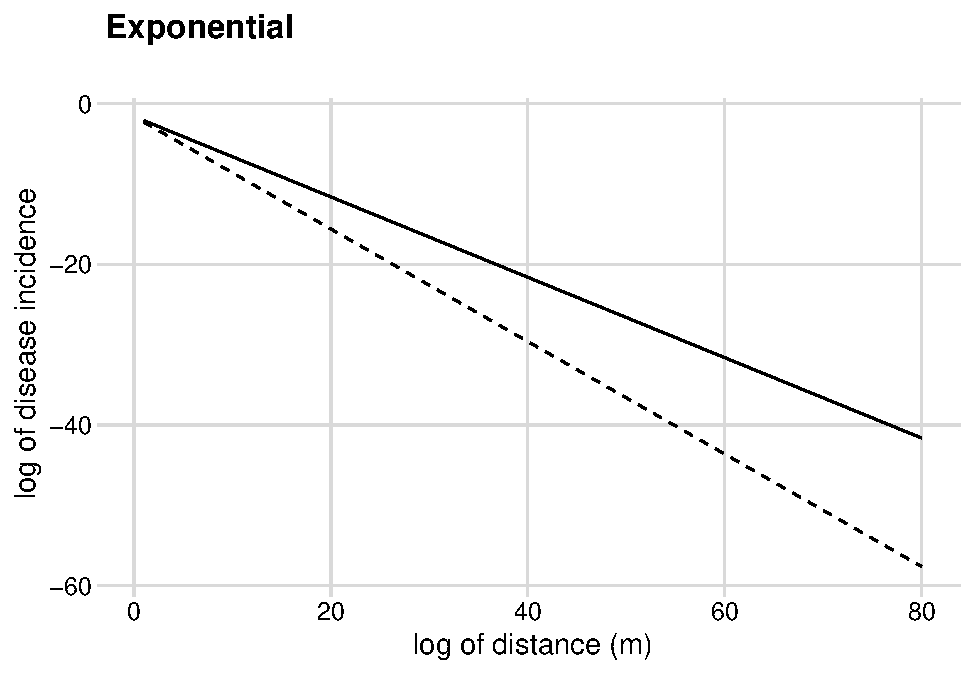
\includegraphics{./spatial-gradients_files/figure-pdf/unnamed-chunk-10-1.pdf}

}

\end{figure}

\hypertarget{gradient-models}{%
\chapter{Gradient models}\label{gradient-models}}

Similar to disease progress curves, models can be fitted empirically to
observed disease gradient curves and provide insights into the
mechanisms of inoculum dispersal and deposition, the source of inoculum,
and the physical processes underlying dispersal.

When modeling disease gradients, the distance is represented by \(x\), a
continuous variable which can be expressed by various units (cm, m, km,
etc). The gradient models, similar to the population dynamics models
(disease progress) are of the \textbf{deterministic} type. The
difference is that, for disease progress curves, disease intensity tends
to increase with increasing time, while in disease gradients the disease
intensity tends to decrease with increasing distance from the source of
inoculum. Two models are most commonly fitted to data on disease
gradients. More details about these models can be obtained it
\href{https://www.apsnet.org/edcenter/disimpactmngmnt/topc/EcologyAndEpidemiologyInR/ModelingDispersalGradients/Pages/default.aspx}{this
tutorial.}

\hypertarget{exponential-model}{%
\subsection{Exponential model}\label{exponential-model}}

The exponential model is also known as Kiyosawa \& Shiyomi model. The
differential of the exponential model is given by

\(\frac{dy}{dx}\) = \(-b_{E}.y\) ,

where \(b_{E}\) is the exponential form of the rate of decline and \(y\)
is the disease intensity. This model suggests that \(y\) (any disease
intensity) is greater close to the source of inoculum, or at the
distance zero. The integral form of the model is given by

\(y = a . e^{-b.x}\) ,

where \(a\) is the disease intensity at the distance zero and \(b\) is
the rate of decline, in this case negative because disease intensity
decreases with the increase of the distance from inoculum source. Let's
make a plot for two disease gradients of varying parameters for this
model.

First we need to load essential packages for programming, customizing
the outputs and defining a global ggplot theme.

\begin{Shaded}
\begin{Highlighting}[]
\FunctionTok{library}\NormalTok{(tidyverse)}
\FunctionTok{library}\NormalTok{(ggthemes)}
\FunctionTok{library}\NormalTok{(patchwork)}
\FunctionTok{library}\NormalTok{(cowplot) }\CommentTok{\# for themes }
\FunctionTok{theme\_set}\NormalTok{(}\FunctionTok{theme\_bw}\NormalTok{(}\AttributeTok{base\_size =} \DecValTok{16}\NormalTok{)) }\CommentTok{\# set global theme}
\end{Highlighting}
\end{Shaded}

Set the parameters for the exponential model with two rates and same
inoculum at the source:

\begin{Shaded}
\begin{Highlighting}[]
\NormalTok{a1 }\OtherTok{\textless{}{-}} \FloatTok{0.2} \CommentTok{\# y at distance zero for gradient 1}
\NormalTok{a2 }\OtherTok{\textless{}{-}} \FloatTok{0.2} \CommentTok{\# y at distance zero for gradient 2}
\NormalTok{b1 }\OtherTok{\textless{}{-}} \FloatTok{0.1} \CommentTok{\# decline rate for gradient 1}
\NormalTok{b2 }\OtherTok{\textless{}{-}} \FloatTok{0.05} \CommentTok{\# decline rate for gradient 2}
\NormalTok{max1 }\OtherTok{\textless{}{-}} \DecValTok{80} \CommentTok{\# maximum distance for gradient 1}
\NormalTok{max2 }\OtherTok{\textless{}{-}} \DecValTok{80} \CommentTok{\# maximum distance for gradient 2}
\NormalTok{dat }\OtherTok{\textless{}{-}} \FunctionTok{data.frame}\NormalTok{(}\AttributeTok{x =} \FunctionTok{seq}\NormalTok{(}\DecValTok{1}\SpecialCharTok{:}\NormalTok{max1), }\AttributeTok{y =} \FunctionTok{seq}\NormalTok{(}\DecValTok{0}\SpecialCharTok{:}\NormalTok{a1))}
\end{Highlighting}
\end{Shaded}

The following code allows to visualize the model predictions.

\begin{Shaded}
\begin{Highlighting}[]
\NormalTok{dat }\SpecialCharTok{|\textgreater{}}
  \FunctionTok{ggplot}\NormalTok{(}\FunctionTok{aes}\NormalTok{(x, y)) }\SpecialCharTok{+}
  \FunctionTok{stat\_function}\NormalTok{(}\AttributeTok{fun =} \ControlFlowTok{function}\NormalTok{(x) a1 }\SpecialCharTok{*} \FunctionTok{exp}\NormalTok{(}\SpecialCharTok{{-}}\NormalTok{b1 }\SpecialCharTok{*}\NormalTok{ x), }\AttributeTok{linetype =} \DecValTok{1}\NormalTok{) }\SpecialCharTok{+}
  \FunctionTok{stat\_function}\NormalTok{(}\AttributeTok{fun =} \ControlFlowTok{function}\NormalTok{(x) a2 }\SpecialCharTok{*} \FunctionTok{exp}\NormalTok{(}\SpecialCharTok{{-}}\NormalTok{b2 }\SpecialCharTok{*}\NormalTok{ x), }\AttributeTok{linetype =} \DecValTok{2}\NormalTok{) }\SpecialCharTok{+}
  \FunctionTok{ylim}\NormalTok{(}\DecValTok{0}\NormalTok{, a1) }\SpecialCharTok{+}
  \FunctionTok{annotate}\NormalTok{(}\StringTok{"text"}\NormalTok{, }\AttributeTok{x =} \DecValTok{20}\NormalTok{, }\AttributeTok{y =} \FloatTok{0.04}\NormalTok{, }\AttributeTok{label =} \StringTok{"b = 0.1"}\NormalTok{) }\SpecialCharTok{+}
  \FunctionTok{annotate}\NormalTok{(}\StringTok{"text"}\NormalTok{, }\AttributeTok{x =} \DecValTok{20}\NormalTok{, }\AttributeTok{y =} \FloatTok{0.10}\NormalTok{, }\AttributeTok{label =} \StringTok{"b = 0.05"}\NormalTok{) }\SpecialCharTok{+}
  \FunctionTok{labs}\NormalTok{(}
    \AttributeTok{title =} \StringTok{"Exponential model"}\NormalTok{,}
    \AttributeTok{subtitle =} \StringTok{""}\NormalTok{,}
    \AttributeTok{x =} \StringTok{"Distance (m)"}\NormalTok{,}
    \AttributeTok{y =} \StringTok{"Disease incidence (proportion)"}
\NormalTok{  )}
\end{Highlighting}
\end{Shaded}

\begin{figure}[H]

{\centering 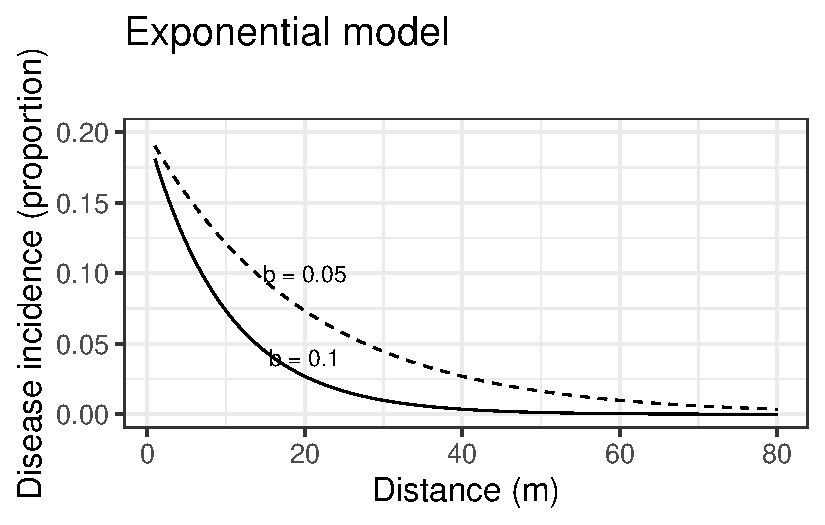
\includegraphics{./spatial-models_files/figure-pdf/unnamed-chunk-6-1.pdf}

}

\end{figure}

\hypertarget{power-law-model}{%
\subsection{Power law model}\label{power-law-model}}

Also known as the modified Gregory's model (Gregory was a pioneer in the
use this model to describe plant disease gradients). In the power law
model, \(Y\) is proportional to the power of the distance, and is given
by:

\(Y = a_{P}.x - b_{P}\)

where \(a_{P}\) and \(b_{P}\) are the two parameters of the power law
model. They differ from the exponential because as closer to \(x\) is to
zero, \(Y\) is indefinitely large (not meaningful biologically).
However, the model can still be useful because it produces realistic
values at any distance \(x\) away from the source. The values of the
\(a_{P}\) parameter should be interpreted in accord to the scale of
\(x\), whether in centimeters or meters. If the distance between the
source and the first measure away from the source is 0.5m, it is so more
appropriate to record the distance in cm than in m or km.

Once \(y\) at the distance zero from the source is undefined when using
the power law model, this is usually modified by the addition of a
positive constant \(C\) in \(x\):

\(Y = a_{P}.(x + C) - b_{P}\)

For this reason, the model is named as the modified power law. Here, the
constant \(C\) is of the same unit of \(x\). At the distance zero, the
positive constant is a term that express the size of the inoculum
source. In other words, the \(a\) parameter is a theoretical value of
\(Y\) at the distance \(1-C\) from the center of the inoculum source.

Let's plot two gradients with two rate parameters for the modified power
law model:

\begin{Shaded}
\begin{Highlighting}[]
\NormalTok{C }\OtherTok{\textless{}{-}} \FloatTok{0.5}
\NormalTok{a1 }\OtherTok{\textless{}{-}} \FloatTok{0.2} \CommentTok{\# y at zero distance for gradient 1}
\NormalTok{a2 }\OtherTok{\textless{}{-}} \FloatTok{0.2} \CommentTok{\# y at zero distance for gradient 2}
\NormalTok{b1 }\OtherTok{\textless{}{-}} \FloatTok{0.5} \CommentTok{\# decline rate for gradient 1}
\NormalTok{b2 }\OtherTok{\textless{}{-}} \FloatTok{0.7} \CommentTok{\# decline rate for gradient 2}
\NormalTok{max1 }\OtherTok{\textless{}{-}} \DecValTok{80} \CommentTok{\# maximum distance for gradient 1}
\NormalTok{max2 }\OtherTok{\textless{}{-}} \DecValTok{80} \CommentTok{\# maximum distance for gradient 2}
\NormalTok{dat2 }\OtherTok{\textless{}{-}} \FunctionTok{data.frame}\NormalTok{(}\AttributeTok{x =} \FunctionTok{seq}\NormalTok{(}\DecValTok{1}\SpecialCharTok{:}\NormalTok{max1), }\AttributeTok{y =} \FunctionTok{seq}\NormalTok{(}\DecValTok{0}\SpecialCharTok{:}\NormalTok{a1))}


\NormalTok{dat2 }\SpecialCharTok{|\textgreater{}}
  \FunctionTok{ggplot}\NormalTok{(}\FunctionTok{aes}\NormalTok{(x, y)) }\SpecialCharTok{+}
  \FunctionTok{stat\_function}\NormalTok{(}\AttributeTok{fun =} \ControlFlowTok{function}\NormalTok{(x) a1 }\SpecialCharTok{*}\NormalTok{ ((x }\SpecialCharTok{+}\NormalTok{ C)}\SpecialCharTok{\^{}{-}}\NormalTok{b1), }\AttributeTok{linetype =} \DecValTok{1}\NormalTok{) }\SpecialCharTok{+}
  \FunctionTok{stat\_function}\NormalTok{(}\AttributeTok{fun =} \ControlFlowTok{function}\NormalTok{(x) a2 }\SpecialCharTok{*}\NormalTok{ ((x }\SpecialCharTok{+}\NormalTok{ C)}\SpecialCharTok{\^{}{-}}\NormalTok{b2), }\AttributeTok{linetype =} \DecValTok{2}\NormalTok{) }\SpecialCharTok{+}
  \FunctionTok{ylim}\NormalTok{(}\DecValTok{0}\NormalTok{, a1 }\SpecialCharTok{{-}} \FloatTok{0.02}\NormalTok{) }\SpecialCharTok{+}
  \FunctionTok{annotate}\NormalTok{(}\StringTok{"text"}\NormalTok{, }\AttributeTok{x =} \DecValTok{20}\NormalTok{, }\AttributeTok{y =} \FloatTok{0.03}\NormalTok{, }\AttributeTok{label =} \StringTok{"b = 0.1"}\NormalTok{) }\SpecialCharTok{+}
  \FunctionTok{annotate}\NormalTok{(}\StringTok{"text"}\NormalTok{, }\AttributeTok{x =} \DecValTok{20}\NormalTok{, }\AttributeTok{y =} \FloatTok{0.06}\NormalTok{, }\AttributeTok{label =} \StringTok{"b = 0.05"}\NormalTok{) }\SpecialCharTok{+}
  \FunctionTok{labs}\NormalTok{(}
    \AttributeTok{title =} \StringTok{"Modified Power Law"}\NormalTok{,}
    \AttributeTok{subtitle =} \StringTok{""}\NormalTok{,}
    \AttributeTok{x =} \StringTok{"Distance (m)"}\NormalTok{,}
    \AttributeTok{y =} \StringTok{"Disease incidence"}
\NormalTok{  )}
\end{Highlighting}
\end{Shaded}

\begin{figure}[H]

{\centering 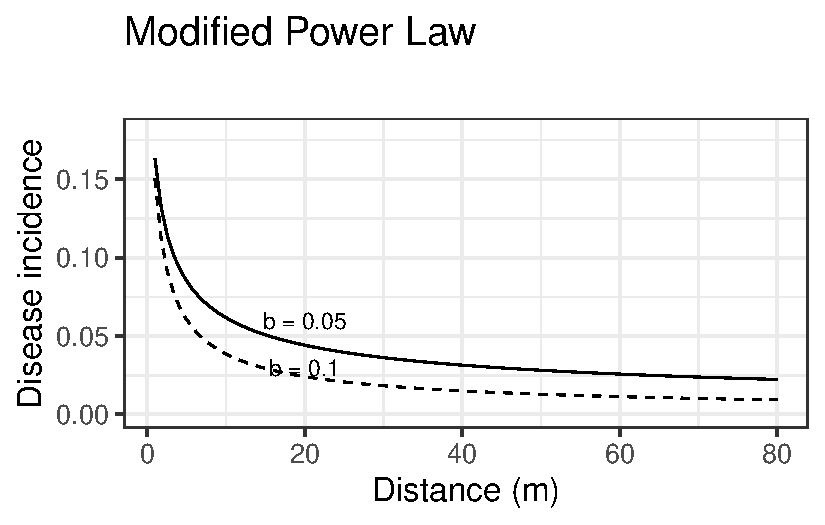
\includegraphics{./spatial-models_files/figure-pdf/unnamed-chunk-8-1.pdf}

}

\end{figure}

The differential equation of the power law model is given by:

\(\frac{dy}{dx}\) = \(\frac{-b_{P}.Y}{x - C}\)

Similar to the exponential model, \(\frac{dy}{dx}\) is proportional to
\(Y\), meaning that the gradient is steeper (more negative) at the
highest disease intensity value, usually closer to the source.

\hypertarget{linearization-of-the-models}{%
\section{Linearization of the
models}\label{linearization-of-the-models}}

\hypertarget{transformations-of-y}{%
\subsection{Transformations of y}\label{transformations-of-y}}

The gradient models, again similar to the temporal disease models, are
\textbf{non linear in their parameters}. The model is intrinsically
linear if transformations are applied (according to the model) in both
sides of the equations. The linear model in its generic state is given
by

\(y* = a* + bx\) ,

where the asterisk in \(a\) indicated that one of the transformations
was applied in \(y\) that produced the linear model. Note that \(a*\) is
the transformed version of the initial disease intensity, which needs to
be returned to the original scale according to the respective
back-transformation. Follows the linearized form of the two most common
gradient models.

\(ln(y) = ln(a_{E}) - b_{E}. x\)

\(ln(y) = ln(a_{P}) - b_{E}. ln(x+C)\)

\hypertarget{plot-for-the-linearized-form-of-models}{%
\subsection{Plot for the linearized form of
models}\label{plot-for-the-linearized-form-of-models}}

Let's visualize the linearization of the exponential model with two
different slopes (gradient 1 and 2). Note that the transformation used
was \(ln(y)\).

Follows the linearization of the modified power law model.

\begin{Shaded}
\begin{Highlighting}[]
\NormalTok{C }\OtherTok{\textless{}{-}} \FloatTok{0.5}
\NormalTok{a1 }\OtherTok{\textless{}{-}} \FloatTok{0.2} \CommentTok{\# y at zero distance for gradient 1}
\NormalTok{a2 }\OtherTok{\textless{}{-}} \FloatTok{0.2} \CommentTok{\# y at zero distance for gradient 2}
\NormalTok{b1 }\OtherTok{\textless{}{-}} \FloatTok{0.5} \CommentTok{\# decline rate for gradient 1}
\NormalTok{b2 }\OtherTok{\textless{}{-}} \FloatTok{0.7} \CommentTok{\# decline rate for gradient 2}
\NormalTok{max1 }\OtherTok{\textless{}{-}} \DecValTok{80} \CommentTok{\# maximum distance for gradient 1}
\NormalTok{max2 }\OtherTok{\textless{}{-}} \DecValTok{80} \CommentTok{\# maximum distance for gradient 2}
\NormalTok{dat2 }\OtherTok{\textless{}{-}} \FunctionTok{data.frame}\NormalTok{(}\AttributeTok{x =} \FunctionTok{seq}\NormalTok{(}\DecValTok{1}\SpecialCharTok{:}\NormalTok{max1), }\AttributeTok{y =} \FunctionTok{seq}\NormalTok{(}\DecValTok{0}\SpecialCharTok{:}\NormalTok{a1))}

\NormalTok{dat2 }\SpecialCharTok{|\textgreater{}}
  \FunctionTok{ggplot}\NormalTok{(}\FunctionTok{aes}\NormalTok{(x, y)) }\SpecialCharTok{+}
  \FunctionTok{stat\_function}\NormalTok{(}\AttributeTok{fun =} \ControlFlowTok{function}\NormalTok{(x) }\FunctionTok{log}\NormalTok{(a1) }\SpecialCharTok{{-}}\NormalTok{ (b1 }\SpecialCharTok{*}\NormalTok{ x), }\AttributeTok{linetype =} \DecValTok{1}\NormalTok{) }\SpecialCharTok{+}
  \FunctionTok{stat\_function}\NormalTok{(}\AttributeTok{fun =} \ControlFlowTok{function}\NormalTok{(x) }\FunctionTok{log}\NormalTok{(a2) }\SpecialCharTok{{-}}\NormalTok{ (b2 }\SpecialCharTok{*}\NormalTok{ x), }\AttributeTok{linetype =} \DecValTok{2}\NormalTok{) }\SpecialCharTok{+}
  \FunctionTok{labs}\NormalTok{(}
    \AttributeTok{title =} \StringTok{"Exponential"}\NormalTok{,}
    \AttributeTok{subtitle =} \StringTok{""}\NormalTok{,}
    \AttributeTok{x =} \StringTok{"log of distance (m)"}\NormalTok{,}
    \AttributeTok{y =} \StringTok{"log of disease incidence"}
\NormalTok{  )}
\end{Highlighting}
\end{Shaded}

\begin{figure}[H]

{\centering 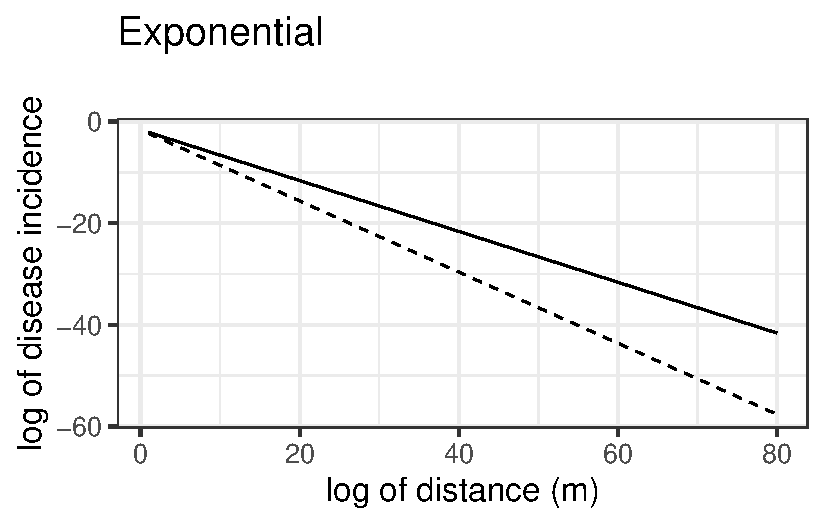
\includegraphics{./spatial-models_files/figure-pdf/unnamed-chunk-10-1.pdf}

}

\end{figure}

Follows the linearization of the modified power law model. Note that the
transformation used was \(ln(y)\) and \(ln(x+C)\) .

\begin{Shaded}
\begin{Highlighting}[]
\NormalTok{C }\OtherTok{\textless{}{-}} \FloatTok{0.5}
\NormalTok{a1 }\OtherTok{\textless{}{-}} \FloatTok{0.2} \CommentTok{\# y at zero distance for gradient 1}
\NormalTok{a2 }\OtherTok{\textless{}{-}} \FloatTok{0.2} \CommentTok{\# y at zero distance for gradient 2}
\NormalTok{b1 }\OtherTok{\textless{}{-}} \FloatTok{0.5} \CommentTok{\# decline rate for gradient 1}
\NormalTok{b2 }\OtherTok{\textless{}{-}} \FloatTok{0.7} \CommentTok{\# decline rate for gradient 2}
\NormalTok{max1 }\OtherTok{\textless{}{-}} \FunctionTok{log}\NormalTok{(}\DecValTok{80}\NormalTok{) }\CommentTok{\# maximum distance for gradient 1}
\NormalTok{max2 }\OtherTok{\textless{}{-}} \FunctionTok{log}\NormalTok{(}\DecValTok{80}\NormalTok{) }\CommentTok{\# maximum distance for gradient 2}
\NormalTok{dat2 }\OtherTok{\textless{}{-}} \FunctionTok{data.frame}\NormalTok{(}\AttributeTok{x =} \FunctionTok{seq}\NormalTok{(}\DecValTok{1}\SpecialCharTok{:}\NormalTok{max1), }\AttributeTok{y =} \FunctionTok{seq}\NormalTok{(}\DecValTok{0}\SpecialCharTok{:}\NormalTok{a1))}

\NormalTok{dat2 }\SpecialCharTok{|\textgreater{}}
  \FunctionTok{ggplot}\NormalTok{(}\FunctionTok{aes}\NormalTok{(x, y)) }\SpecialCharTok{+}
  \FunctionTok{stat\_function}\NormalTok{(}\AttributeTok{fun =} \ControlFlowTok{function}\NormalTok{(x) }\FunctionTok{log}\NormalTok{(a1) }\SpecialCharTok{{-}}\NormalTok{ (b1 }\SpecialCharTok{*} \FunctionTok{log}\NormalTok{(x }\SpecialCharTok{+}\NormalTok{ C)), }\AttributeTok{linetype =} \DecValTok{1}\NormalTok{) }\SpecialCharTok{+}
  \FunctionTok{stat\_function}\NormalTok{(}\AttributeTok{fun =} \ControlFlowTok{function}\NormalTok{(x) }\FunctionTok{log}\NormalTok{(a2) }\SpecialCharTok{{-}}\NormalTok{ (b2 }\SpecialCharTok{*} \FunctionTok{log}\NormalTok{(x }\SpecialCharTok{+}\NormalTok{ C)), }\AttributeTok{linetype =} \DecValTok{2}\NormalTok{) }\SpecialCharTok{+}
  \FunctionTok{labs}\NormalTok{(}
    \AttributeTok{title =} \StringTok{"Modified Power Law"}\NormalTok{,}
    \AttributeTok{subtitle =} \StringTok{""}\NormalTok{,}
    \AttributeTok{x =} \StringTok{"log of distance (m)"}\NormalTok{,}
    \AttributeTok{y =} \StringTok{"log of disease incidence"}
\NormalTok{  )}
\end{Highlighting}
\end{Shaded}

\begin{figure}[H]

{\centering \includegraphics{./spatial-models_files/figure-pdf/unnamed-chunk-12-1.pdf}

}

\end{figure}

\hypertarget{fitting-gradient-models}{%
\chapter{Fitting gradient models}\label{fitting-gradient-models}}

\begin{tcolorbox}[enhanced jigsaw, rightrule=.15mm, left=2mm, breakable, colframe=quarto-callout-note-color-frame, toprule=.15mm, leftrule=.75mm, bottomrule=.15mm, colback=white, arc=.35mm, opacityback=0]
\begin{minipage}[t]{5.5mm}
\textcolor{quarto-callout-note-color}{\faInfo}
\end{minipage}%
\begin{minipage}[t]{\textwidth - 5.5mm}
This is a work in progress that is currently undergoing heavy technical
editing and copy-editing\end{minipage}%
\end{tcolorbox}

\begin{Shaded}
\begin{Highlighting}[]
\FunctionTok{library}\NormalTok{(tidyverse)}
\FunctionTok{library}\NormalTok{(ggthemes)}
\FunctionTok{library}\NormalTok{(patchwork)}
\FunctionTok{library}\NormalTok{(cowplot) }\CommentTok{\# for themes }
\FunctionTok{theme\_set}\NormalTok{(}\FunctionTok{theme\_bw}\NormalTok{(}\AttributeTok{base\_size =} \DecValTok{16}\NormalTok{)) }\CommentTok{\# set global theme}
\end{Highlighting}
\end{Shaded}

The hypothetical data below shows a gradient for the number of lesions
counted at varying distances in meters from the source. Let's create two
vectors, one for the distances \(x\) and the other for the lesion count
\(Y\), and then a dataframe by combining the two vectors.

\begin{Shaded}
\begin{Highlighting}[]
\CommentTok{\# create the two vectors}
\NormalTok{x }\OtherTok{\textless{}{-}} \FunctionTok{c}\NormalTok{(}\FloatTok{0.8}\NormalTok{, }\FloatTok{1.6}\NormalTok{, }\FloatTok{2.4}\NormalTok{, }\FloatTok{3.2}\NormalTok{, }\DecValTok{4}\NormalTok{, }\FloatTok{7.2}\NormalTok{, }\DecValTok{12}\NormalTok{, }\FloatTok{15.2}\NormalTok{, }\FloatTok{21.6}\NormalTok{, }\FloatTok{28.8}\NormalTok{)}
\NormalTok{Y }\OtherTok{\textless{}{-}} \FunctionTok{c}\NormalTok{(}\FloatTok{184.9}\NormalTok{, }\FloatTok{113.3}\NormalTok{, }\FloatTok{113.3}\NormalTok{, }\FloatTok{64.1}\NormalTok{, }\DecValTok{25}\NormalTok{, }\DecValTok{8}\NormalTok{, }\FloatTok{4.3}\NormalTok{, }\FloatTok{2.5}\NormalTok{, }\DecValTok{1}\NormalTok{, }\FloatTok{0.8}\NormalTok{)}
\NormalTok{grad1 }\OtherTok{\textless{}{-}} \FunctionTok{data.frame}\NormalTok{(x, Y) }\CommentTok{\# create the dataframe}
\NormalTok{grad1 }\CommentTok{\# show the gradient}
\end{Highlighting}
\end{Shaded}

\begin{verbatim}
      x     Y
1   0.8 184.9
2   1.6 113.3
3   2.4 113.3
4   3.2  64.1
5   4.0  25.0
6   7.2   8.0
7  12.0   4.3
8  15.2   2.5
9  21.6   1.0
10 28.8   0.8
\end{verbatim}

\hypertarget{visualize-the-gradient}{%
\section{Visualize the gradient}\label{visualize-the-gradient}}

\begin{Shaded}
\begin{Highlighting}[]
\NormalTok{grad1 }\SpecialCharTok{|\textgreater{}} 
  \FunctionTok{ggplot}\NormalTok{(}\FunctionTok{aes}\NormalTok{(x, Y))}\SpecialCharTok{+}
  \FunctionTok{geom\_point}\NormalTok{()}\SpecialCharTok{+}
  \FunctionTok{geom\_line}\NormalTok{()}\SpecialCharTok{+}
  \FunctionTok{labs}\NormalTok{(}\AttributeTok{y =} \StringTok{"Lesion count"}\NormalTok{,}
       \AttributeTok{x =} \StringTok{"Distance (m)"}\NormalTok{)}
\end{Highlighting}
\end{Shaded}

\begin{figure}[H]

{\centering \includegraphics{./spatial-fitting_files/figure-pdf/unnamed-chunk-6-1.pdf}

}

\end{figure}

\hypertarget{linear-regression-1}{%
\chapter{Linear regression}\label{linear-regression-1}}

A linear regression model is fitted to the transformed variables
according to the model. The higher the coefficient of determination, the
better is the fit of the model to the data.

Exponential model

\begin{Shaded}
\begin{Highlighting}[]
\NormalTok{reg\_exp }\OtherTok{\textless{}{-}} \FunctionTok{lm}\NormalTok{(}\FunctionTok{log}\NormalTok{(Y) }\SpecialCharTok{\textasciitilde{}}\NormalTok{ x, }\AttributeTok{data =}\NormalTok{ grad1)}
\FunctionTok{summary}\NormalTok{(reg\_exp)}
\end{Highlighting}
\end{Shaded}

\begin{verbatim}

Call:
lm(formula = log(Y) ~ x, data = grad1)

Residuals:
     Min       1Q   Median       3Q      Max 
-1.04868 -0.58973 -0.00144  0.59572  0.99554 

Coefficients:
            Estimate Std. Error t value Pr(>|t|)    
(Intercept)  4.57705    0.35222  12.995 1.17e-06 ***
x           -0.20124    0.02656  -7.576 6.45e-05 ***
---
Signif. codes:  0 '***' 0.001 '**' 0.01 '*' 0.05 '.' 0.1 ' ' 1

Residual standard error: 0.7612 on 8 degrees of freedom
Multiple R-squared:  0.8777,    Adjusted R-squared:  0.8624 
F-statistic: 57.39 on 1 and 8 DF,  p-value: 6.45e-05
\end{verbatim}

Power law model with \(C = 0\).

\begin{Shaded}
\begin{Highlighting}[]
\NormalTok{reg\_p }\OtherTok{\textless{}{-}} \FunctionTok{lm}\NormalTok{(}\FunctionTok{log}\NormalTok{(Y) }\SpecialCharTok{\textasciitilde{}} \FunctionTok{log}\NormalTok{(x), }\AttributeTok{data =}\NormalTok{ grad1)}
\FunctionTok{summary}\NormalTok{(reg\_p)}
\end{Highlighting}
\end{Shaded}

\begin{verbatim}

Call:
lm(formula = log(Y) ~ log(x), data = grad1)

Residuals:
     Min       1Q   Median       3Q      Max 
-0.72281 -0.11989 -0.03146  0.08755  0.65267 

Coefficients:
            Estimate Std. Error t value Pr(>|t|)    
(Intercept)   5.5638     0.2456   22.66 1.53e-08 ***
log(x)       -1.6978     0.1191  -14.26 5.71e-07 ***
---
Signif. codes:  0 '***' 0.001 '**' 0.01 '*' 0.05 '.' 0.1 ' ' 1

Residual standard error: 0.4235 on 8 degrees of freedom
Multiple R-squared:  0.9621,    Adjusted R-squared:  0.9574 
F-statistic: 203.3 on 1 and 8 DF,  p-value: 5.71e-07
\end{verbatim}

Power law model with \(C = 0.4\).

\begin{Shaded}
\begin{Highlighting}[]
\NormalTok{reg\_pm }\OtherTok{\textless{}{-}} \FunctionTok{lm}\NormalTok{(}\FunctionTok{log}\NormalTok{(Y) }\SpecialCharTok{\textasciitilde{}} \FunctionTok{log}\NormalTok{(x }\SpecialCharTok{+} \FloatTok{0.4}\NormalTok{), }\AttributeTok{data =}\NormalTok{ grad1)}
\FunctionTok{summary}\NormalTok{(reg\_pm)}
\end{Highlighting}
\end{Shaded}

\begin{verbatim}

Call:
lm(formula = log(Y) ~ log(x + 0.4), data = grad1)

Residuals:
     Min       1Q   Median       3Q      Max 
-0.53733 -0.17258 -0.03646  0.08450  0.56928 

Coefficients:
             Estimate Std. Error t value Pr(>|t|)    
(Intercept)    6.1007     0.2283   26.73 4.13e-09 ***
log(x + 0.4)  -1.8841     0.1084  -17.38 1.22e-07 ***
---
Signif. codes:  0 '***' 0.001 '**' 0.01 '*' 0.05 '.' 0.1 ' ' 1

Residual standard error: 0.3495 on 8 degrees of freedom
Multiple R-squared:  0.9742,    Adjusted R-squared:  0.971 
F-statistic: 302.2 on 1 and 8 DF,  p-value: 1.223e-07
\end{verbatim}

Graphs for the fitted models

Exponential

\begin{Shaded}
\begin{Highlighting}[]
\NormalTok{grad1 }\SpecialCharTok{|\textgreater{}} 
  \FunctionTok{ggplot}\NormalTok{(}\FunctionTok{aes}\NormalTok{(x, }\FunctionTok{log}\NormalTok{(Y)))}\SpecialCharTok{+}
  \FunctionTok{geom\_point}\NormalTok{()}\SpecialCharTok{+}
  \FunctionTok{geom\_line}\NormalTok{()}\SpecialCharTok{+}
  \FunctionTok{geom\_abline}\NormalTok{(}\AttributeTok{slope =} \FunctionTok{coef}\NormalTok{(reg\_exp)[[}\DecValTok{2}\NormalTok{]], }\AttributeTok{intercept =} \FunctionTok{coef}\NormalTok{(reg\_exp)[[}\DecValTok{1}\NormalTok{]])}\SpecialCharTok{+}
 \FunctionTok{labs}\NormalTok{(}\AttributeTok{y =} \StringTok{"Log of Lesion count"}\NormalTok{,}
       \AttributeTok{x =} \StringTok{"Distance (m)"}\NormalTok{)}
\end{Highlighting}
\end{Shaded}

\begin{figure}[H]

{\centering \includegraphics{./spatial-fitting_files/figure-pdf/unnamed-chunk-14-1.pdf}

}

\end{figure}

Power law model

\begin{Shaded}
\begin{Highlighting}[]
\NormalTok{grad1 }\SpecialCharTok{|\textgreater{}} 
  \FunctionTok{ggplot}\NormalTok{(}\FunctionTok{aes}\NormalTok{(}\FunctionTok{log}\NormalTok{(x), }\FunctionTok{log}\NormalTok{(Y)))}\SpecialCharTok{+}
  \FunctionTok{geom\_point}\NormalTok{()}\SpecialCharTok{+}
  \FunctionTok{geom\_line}\NormalTok{()}\SpecialCharTok{+}
  \FunctionTok{geom\_abline}\NormalTok{(}\AttributeTok{slope =} \FunctionTok{coef}\NormalTok{(reg\_p)[[}\DecValTok{2}\NormalTok{]], }\AttributeTok{intercept =} \FunctionTok{coef}\NormalTok{(reg\_p)[[}\DecValTok{1}\NormalTok{]])}\SpecialCharTok{+}
 \FunctionTok{labs}\NormalTok{(}\AttributeTok{y =} \StringTok{"Log of Lesion count"}\NormalTok{,}
       \AttributeTok{x =} \StringTok{"Log of distance"}\NormalTok{)}
\end{Highlighting}
\end{Shaded}

\begin{figure}[H]

{\centering \includegraphics{./spatial-fitting_files/figure-pdf/unnamed-chunk-16-1.pdf}

}

\end{figure}

Modified power law model

\begin{Shaded}
\begin{Highlighting}[]
\NormalTok{grad1 }\SpecialCharTok{|\textgreater{}} 
  \FunctionTok{ggplot}\NormalTok{(}\FunctionTok{aes}\NormalTok{(}\FunctionTok{log}\NormalTok{(x}\FloatTok{+0.4}\NormalTok{), }\FunctionTok{log}\NormalTok{(Y)))}\SpecialCharTok{+}
  \FunctionTok{geom\_point}\NormalTok{()}\SpecialCharTok{+}
  \FunctionTok{geom\_line}\NormalTok{()}\SpecialCharTok{+}
  \FunctionTok{geom\_abline}\NormalTok{(}\AttributeTok{slope =} \FunctionTok{coef}\NormalTok{(reg\_pm)[[}\DecValTok{2}\NormalTok{]], }\AttributeTok{intercept =} \FunctionTok{coef}\NormalTok{(reg\_pm)[[}\DecValTok{1}\NormalTok{]])}\SpecialCharTok{+}
 \FunctionTok{labs}\NormalTok{(}\AttributeTok{y =} \StringTok{"Log of Lesion count"}\NormalTok{,}
       \AttributeTok{x =} \StringTok{"Log of distance (m)"}\NormalTok{)}
\end{Highlighting}
\end{Shaded}

\begin{figure}[H]

{\centering \includegraphics{./spatial-fitting_files/figure-pdf/unnamed-chunk-18-1.pdf}

}

\end{figure}

Conclusion: The modified power law model provided the best fit.

\hypertarget{spatial-patterns}{%
\chapter{Spatial patterns}\label{spatial-patterns}}

\begin{tcolorbox}[enhanced jigsaw, rightrule=.15mm, left=2mm, breakable, colframe=quarto-callout-note-color-frame, toprule=.15mm, leftrule=.75mm, bottomrule=.15mm, colback=white, arc=.35mm, opacityback=0]
\begin{minipage}[t]{5.5mm}
\textcolor{quarto-callout-note-color}{\faInfo}
\end{minipage}%
\begin{minipage}[t]{\textwidth - 5.5mm}
This is a work in progress that is currently undergoing heavy technical
editing and copy-editing\end{minipage}%
\end{tcolorbox}

\hypertarget{definitions}{%
\section{Definitions}\label{definitions}}

A spatial disease pattern can be defined as the arrangement of diseased
entities relative to each other and to the architecture of the host crop
(Madden et al. 2017a). Such arrangement is the realization of the
underlying dispersal of the pathogen, from one or several sources within
and/or outside the area of interest, under the influence of physical,
biological and environmental factors.

The study of spatial patterns is conducted at a specific time or
multiple times during the epidemic. When assessed multiple times, both
spatial and temporal processes can be characterized. Because epidemics
change over time, it is expected that spatial patterns are not constant
but change over time as well. Usually, plant pathologists are interested
in determining spatial patterns at one or various spatial scales,
depending on the objective of the study. The scale of interest may be a
leaf or root, plant, field, municipality, state, country or even
intercontinental area. The diseased units observed may vary from lesions
on a single leaf to diseased fields in a large production region.

The patterns can be classified into two main types that occur naturally:
\textbf{random} or \textbf{aggregated}. The random pattern originates
because the chances for the units (leaf, plant, crop) to be infected are
equal and low, and are largely independent from each other. In
aggregated spatial patterns, such chances are unequal and there is
dependency among the units. For example, a healthy unit close to a
diseased unit is at higher risk than more distant units.

Let's simulate in R two vectors (x,y) for the positions of diseased
unitss that follow a random or an aggregated pattern. For the random
pattern, we use \texttt{runif}, a function which generates random
deviates from the uniform distribution.

\begin{Shaded}
\begin{Highlighting}[]
\FunctionTok{set.seed}\NormalTok{(}\DecValTok{123}\NormalTok{)          }\CommentTok{\# for reproducibility}
\NormalTok{x }\OtherTok{\textless{}{-}} \FunctionTok{runif}\NormalTok{(}\DecValTok{50}\NormalTok{, }\DecValTok{0}\NormalTok{, }\DecValTok{30}\NormalTok{)  }\CommentTok{\# x vector}
\NormalTok{y }\OtherTok{\textless{}{-}} \FunctionTok{runif}\NormalTok{(}\DecValTok{50}\NormalTok{, }\DecValTok{0}\NormalTok{, }\DecValTok{30}\NormalTok{)  }\CommentTok{\# y vector}
\NormalTok{dat }\OtherTok{\textless{}{-}} \FunctionTok{data.frame}\NormalTok{(x,y) }\CommentTok{\# dataframe for plotting}
\end{Highlighting}
\end{Shaded}

Now, the plot to visualize the random pattern.

\begin{Shaded}
\begin{Highlighting}[]
\FunctionTok{library}\NormalTok{(tidyverse) }
\FunctionTok{library}\NormalTok{(ggthemes)}
\FunctionTok{theme\_set}\NormalTok{(}\FunctionTok{theme\_few}\NormalTok{())}

\NormalTok{pr }\OtherTok{\textless{}{-}}\NormalTok{ dat }\SpecialCharTok{|\textgreater{}} \CommentTok{\# R base pipe operator}
  \FunctionTok{ggplot}\NormalTok{(}\FunctionTok{aes}\NormalTok{(x, y))}\SpecialCharTok{+}
  \FunctionTok{geom\_point}\NormalTok{(}\AttributeTok{size =}\DecValTok{3}\NormalTok{, }
             \AttributeTok{color =} \StringTok{"darkred"}\NormalTok{)}\SpecialCharTok{+}
  \FunctionTok{ylim}\NormalTok{(}\DecValTok{0}\NormalTok{,}\DecValTok{30}\NormalTok{)}\SpecialCharTok{+}
  \FunctionTok{xlim}\NormalTok{(}\DecValTok{0}\NormalTok{,}\DecValTok{30}\NormalTok{)}\SpecialCharTok{+}
  \FunctionTok{coord\_fixed}\NormalTok{()}\SpecialCharTok{+}
  \FunctionTok{labs}\NormalTok{(}\AttributeTok{x =} \StringTok{"Distance x"}\NormalTok{, }\AttributeTok{y =} \StringTok{"Distance y"}\NormalTok{, }
       \AttributeTok{title =} \StringTok{"Random"}\NormalTok{)}
\NormalTok{pr}
\end{Highlighting}
\end{Shaded}

\begin{figure}[H]

{\centering \includegraphics{./spatial-patterns_files/figure-pdf/unnamed-chunk-4-1.pdf}

}

\end{figure}

Now, we can generate new x and y vectors using \texttt{rnbinom} function
which allows generating values for the negative binomial distribution
(which should give rise to aggregated patterns) with parameters
\texttt{size} and \texttt{prob}. Let's simulate 50 values with mean 12
and size 20 as dispersal parameter.

\begin{Shaded}
\begin{Highlighting}[]
\NormalTok{x }\OtherTok{\textless{}{-}} \FunctionTok{rnbinom}\NormalTok{(}\AttributeTok{n =} \DecValTok{50}\NormalTok{, }\AttributeTok{mu =} \DecValTok{12}\NormalTok{, }\AttributeTok{size =} \DecValTok{20}\NormalTok{)}
\NormalTok{y }\OtherTok{\textless{}{-}} \FunctionTok{rnbinom}\NormalTok{(}\AttributeTok{n =} \DecValTok{50}\NormalTok{, }\AttributeTok{mu =} \DecValTok{5}\NormalTok{, }\AttributeTok{size =} \DecValTok{20}\NormalTok{)}
\NormalTok{dat2 }\OtherTok{\textless{}{-}} \FunctionTok{data.frame}\NormalTok{(x, y)}
\end{Highlighting}
\end{Shaded}

This should give us an aggregated pattern.

\begin{Shaded}
\begin{Highlighting}[]
\NormalTok{pag }\OtherTok{\textless{}{-}}\NormalTok{ dat2 }\SpecialCharTok{|\textgreater{}}
  \FunctionTok{ggplot}\NormalTok{(}\FunctionTok{aes}\NormalTok{(x, y))}\SpecialCharTok{+}
  \FunctionTok{geom\_point}\NormalTok{(}\AttributeTok{size =} \DecValTok{3}\NormalTok{, }\AttributeTok{color =} \StringTok{"darkred"}\NormalTok{)}\SpecialCharTok{+}
  \FunctionTok{ylim}\NormalTok{(}\DecValTok{0}\NormalTok{,}\DecValTok{30}\NormalTok{)}\SpecialCharTok{+}
  \FunctionTok{xlim}\NormalTok{(}\DecValTok{0}\NormalTok{,}\DecValTok{30}\NormalTok{)}\SpecialCharTok{+}
  \FunctionTok{coord\_fixed}\NormalTok{()}\SpecialCharTok{+}
  \FunctionTok{labs}\NormalTok{(}\AttributeTok{x =} \StringTok{"Distance x"}\NormalTok{, }\AttributeTok{y =} \StringTok{"Distance y"}\NormalTok{, }
       \AttributeTok{title =} \StringTok{"Aggregated"}\NormalTok{)}
\NormalTok{pag}
\end{Highlighting}
\end{Shaded}

\begin{figure}[H]

{\centering \includegraphics{./spatial-patterns_files/figure-pdf/unnamed-chunk-8-1.pdf}

}

\end{figure}

A rare pattern found in nature is the regular pattern, but it may be
generated artificially by the man when conducting experimentation.
Follows a code to produce the regular pattern.

\begin{Shaded}
\begin{Highlighting}[]
\NormalTok{x }\OtherTok{\textless{}{-}} \FunctionTok{rep}\NormalTok{(}\FunctionTok{c}\NormalTok{(}\DecValTok{0}\NormalTok{,}\DecValTok{5}\NormalTok{,}\DecValTok{10}\NormalTok{,}\DecValTok{15}\NormalTok{,}\DecValTok{20}\NormalTok{, }\DecValTok{25}\NormalTok{, }\DecValTok{30}\NormalTok{, }\DecValTok{35}\NormalTok{, }\DecValTok{40}\NormalTok{, }\DecValTok{45}\NormalTok{), }\DecValTok{5}\NormalTok{) }
\NormalTok{y }\OtherTok{\textless{}{-}} \FunctionTok{rep}\NormalTok{(}\FunctionTok{c}\NormalTok{(}\DecValTok{0}\NormalTok{, }\DecValTok{5}\NormalTok{, }\DecValTok{10}\NormalTok{, }\DecValTok{15}\NormalTok{, }\DecValTok{20}\NormalTok{, }\DecValTok{25}\NormalTok{, }\DecValTok{30}\NormalTok{, }\DecValTok{35}\NormalTok{, }\DecValTok{40}\NormalTok{, }\DecValTok{45}\NormalTok{), }\AttributeTok{each =} \DecValTok{10}\NormalTok{)}
\NormalTok{dat3 }\OtherTok{\textless{}{-}} \FunctionTok{data.frame}\NormalTok{(x, y)}

\NormalTok{preg }\OtherTok{\textless{}{-}}\NormalTok{ dat3 }\SpecialCharTok{|\textgreater{}}
  \FunctionTok{ggplot}\NormalTok{(}\FunctionTok{aes}\NormalTok{(x, y))}\SpecialCharTok{+}
  \FunctionTok{geom\_point}\NormalTok{(}\AttributeTok{size =} \DecValTok{3}\NormalTok{, }\AttributeTok{color =} \StringTok{"darkred"}\NormalTok{)}\SpecialCharTok{+}
  \FunctionTok{ylim}\NormalTok{(}\DecValTok{0}\NormalTok{,}\DecValTok{30}\NormalTok{)}\SpecialCharTok{+}
  \FunctionTok{xlim}\NormalTok{(}\DecValTok{0}\NormalTok{,}\DecValTok{30}\NormalTok{)}\SpecialCharTok{+}
  \FunctionTok{coord\_fixed}\NormalTok{()}\SpecialCharTok{+}
  \FunctionTok{labs}\NormalTok{(}\AttributeTok{x =} \StringTok{"Distance x"}\NormalTok{, }\AttributeTok{y =} \StringTok{"Distance y"}\NormalTok{, }
       \AttributeTok{title =} \StringTok{"Regular"}\NormalTok{)}
\NormalTok{preg}
\end{Highlighting}
\end{Shaded}

\begin{verbatim}
Warning: Removed 51 rows containing missing values (geom_point).
\end{verbatim}

\begin{figure}[H]

{\centering \includegraphics{./spatial-patterns_files/figure-pdf/unnamed-chunk-10-1.pdf}

}

\end{figure}

\begin{Shaded}
\begin{Highlighting}[]
\FunctionTok{library}\NormalTok{(patchwork)}

\NormalTok{preg }\SpecialCharTok{+}\NormalTok{ pr }\SpecialCharTok{+}\NormalTok{ pag}
\end{Highlighting}
\end{Shaded}

\begin{figure}[H]

{\centering \includegraphics{./spatial-patterns_files/figure-pdf/unnamed-chunk-12-1.pdf}

}

\end{figure}

\begin{Shaded}
\begin{Highlighting}[]
\FunctionTok{ggsave}\NormalTok{(}\StringTok{"imgs/spatial.png"}\NormalTok{, }\AttributeTok{width =} \DecValTok{10}\NormalTok{, }\AttributeTok{height =} \DecValTok{4}\NormalTok{)}
\end{Highlighting}
\end{Shaded}

We can create an animation showing the three patterns using
\emph{gganimate} package

\begin{Shaded}
\begin{Highlighting}[]
\NormalTok{rand }\OtherTok{\textless{}{-}}\NormalTok{ dat }\SpecialCharTok{|\textgreater{}} 
  \FunctionTok{mutate}\NormalTok{(}\AttributeTok{i =} \StringTok{"random"}\NormalTok{)}

\NormalTok{agg }\OtherTok{\textless{}{-}}\NormalTok{ dat2 }\SpecialCharTok{|\textgreater{}} 
  \FunctionTok{mutate}\NormalTok{(}\AttributeTok{i =} \StringTok{"aggregated"}\NormalTok{)}

\NormalTok{reg }\OtherTok{\textless{}{-}}\NormalTok{ dat3 }\SpecialCharTok{|\textgreater{}} 
  \FunctionTok{mutate}\NormalTok{(}\AttributeTok{i =} \StringTok{"regular"}\NormalTok{)}

\NormalTok{patterns }\OtherTok{\textless{}{-}} \FunctionTok{rbind}\NormalTok{(agg, rand, reg)}

\FunctionTok{library}\NormalTok{(gganimate)}

\NormalTok{patterns }\SpecialCharTok{|\textgreater{}} 
\FunctionTok{ggplot}\NormalTok{(}\FunctionTok{aes}\NormalTok{(x, y, }\AttributeTok{color =} \FunctionTok{factor}\NormalTok{(i)))}\SpecialCharTok{+}
  \FunctionTok{geom\_point}\NormalTok{(}\AttributeTok{size =} \DecValTok{4}\NormalTok{, }\AttributeTok{color =} \StringTok{"darkred"}\NormalTok{)}\SpecialCharTok{+}
  \FunctionTok{coord\_fixed}\NormalTok{()}\SpecialCharTok{+}
  \FunctionTok{ylim}\NormalTok{(}\DecValTok{0}\NormalTok{,}\DecValTok{25}\NormalTok{)}\SpecialCharTok{+}
  \FunctionTok{xlim}\NormalTok{(}\DecValTok{0}\NormalTok{,}\DecValTok{25}\NormalTok{)}\SpecialCharTok{+}
  \FunctionTok{transition\_states}\NormalTok{(i)}\SpecialCharTok{+}
  \FunctionTok{theme\_few}\NormalTok{()}\SpecialCharTok{+}
  \FunctionTok{ggtitle}\NormalTok{(}\StringTok{\textquotesingle{}Pattern: \{closest\_state\}\textquotesingle{}}\NormalTok{)}
\FunctionTok{anim\_save}\NormalTok{(}\StringTok{"imgs/patterns.gif"}\NormalTok{)}
\end{Highlighting}
\end{Shaded}

\includegraphics{./imgs/patterns.gif}

\hypertarget{spatiotemporal}{%
\section{Spatiotemporal}\label{spatiotemporal}}

The location of diseased plants can be assessed over time and so we can
appraise both the progress and pattern of the epidemics. Let's visualize
spatial data collected from actual epidemics monitored (plant is
diseased or not diseased) during six times during the epidemics. The
data is available in the \texttt{epiphy} R package. Let's use only one
variety and one irrigation type.

\begin{Shaded}
\begin{Highlighting}[]
\FunctionTok{library}\NormalTok{(epiphy)}
\NormalTok{tswv\_1928 }\OtherTok{\textless{}{-}}\NormalTok{ tomato\_tswv}\SpecialCharTok{$}\NormalTok{field\_1928}

\NormalTok{tswv\_1928 }\SpecialCharTok{|\textgreater{}}
  \FunctionTok{filter}\NormalTok{(variety }\SpecialCharTok{==} \StringTok{"Burwood{-}Prize"}\SpecialCharTok{\&}
\NormalTok{         irrigation }\SpecialCharTok{==} \StringTok{"trenches"}\NormalTok{) }\SpecialCharTok{|\textgreater{}} 
  \FunctionTok{ggplot}\NormalTok{(}\FunctionTok{aes}\NormalTok{(x, y, }\AttributeTok{color =} \FunctionTok{factor}\NormalTok{(i)))}\SpecialCharTok{+}
  \FunctionTok{geom\_point}\NormalTok{(}\FunctionTok{aes}\NormalTok{(}\AttributeTok{group =} \FunctionTok{seq\_along}\NormalTok{(}\FunctionTok{factor}\NormalTok{(t))), }\AttributeTok{size =}\DecValTok{2}\NormalTok{)}\SpecialCharTok{+}
  \FunctionTok{coord\_fixed}\NormalTok{()}\SpecialCharTok{+}
  \FunctionTok{scale\_color\_manual}\NormalTok{(}\AttributeTok{values =} \FunctionTok{c}\NormalTok{(}\StringTok{"grey70"}\NormalTok{, }\StringTok{"darkred"}\NormalTok{))}\SpecialCharTok{+}
  \FunctionTok{labs}\NormalTok{(}\AttributeTok{fill =} \StringTok{"Status"}\NormalTok{, }\AttributeTok{title =} \StringTok{""}\NormalTok{)}\SpecialCharTok{+}
  \FunctionTok{theme\_void}\NormalTok{()}\SpecialCharTok{+}
  \FunctionTok{facet\_wrap}\NormalTok{(}\SpecialCharTok{\textasciitilde{}}\NormalTok{ t, }\AttributeTok{nrow =}\DecValTok{1}\NormalTok{)}
\end{Highlighting}
\end{Shaded}

\begin{figure}[H]

{\centering \includegraphics{./spatial-patterns_files/figure-pdf/unnamed-chunk-16-1.pdf}

}

\end{figure}

We can use the \emph{gganimate} package to visualize the spatiotemporal
dynamics of the epidemics.

\begin{Shaded}
\begin{Highlighting}[]
\FunctionTok{library}\NormalTok{(gganimate)}
\NormalTok{tswv\_1928 }\SpecialCharTok{|\textgreater{}}
  \FunctionTok{filter}\NormalTok{(variety }\SpecialCharTok{==} \StringTok{"Burwood{-}Prize"}\SpecialCharTok{\&}
\NormalTok{         irrigation }\SpecialCharTok{==} \StringTok{"trenches"}\NormalTok{) }\SpecialCharTok{|\textgreater{}} 
  \FunctionTok{ggplot}\NormalTok{(}\FunctionTok{aes}\NormalTok{(y, x, }\AttributeTok{color =} \FunctionTok{factor}\NormalTok{(i)))}\SpecialCharTok{+}
  \FunctionTok{geom\_point}\NormalTok{(}\FunctionTok{aes}\NormalTok{(}\AttributeTok{group =} \FunctionTok{seq\_along}\NormalTok{(}\FunctionTok{factor}\NormalTok{(t))), }\AttributeTok{size =}\DecValTok{5}\NormalTok{)}\SpecialCharTok{+}
  \FunctionTok{scale\_color\_manual}\NormalTok{(}\AttributeTok{values =} \FunctionTok{c}\NormalTok{(}\StringTok{"gray70"}\NormalTok{, }\StringTok{"darkred"}\NormalTok{))}\SpecialCharTok{+}
  \FunctionTok{labs}\NormalTok{(}\AttributeTok{fill =} \StringTok{"Status"}\NormalTok{, }\AttributeTok{title =} \StringTok{""}\NormalTok{)}\SpecialCharTok{+}
  \FunctionTok{theme\_void}\NormalTok{()}\SpecialCharTok{+}
  \FunctionTok{coord\_fixed}\NormalTok{()}\SpecialCharTok{+}
  \FunctionTok{transition\_states}\NormalTok{(t,}
                  \AttributeTok{transition\_length =} \DecValTok{1}\NormalTok{,}
                    \AttributeTok{state\_length =} \DecValTok{1}\NormalTok{)}\SpecialCharTok{+}
   \FunctionTok{ggtitle}\NormalTok{(}\StringTok{\textquotesingle{}Assessment time: \{closest\_state\}\textquotesingle{}}\NormalTok{)}
\FunctionTok{anim\_save}\NormalTok{(}\StringTok{"imgs/spatiotemporal.gif"}\NormalTok{)}
\end{Highlighting}
\end{Shaded}

\includegraphics[width=7.13542in,height=\textheight]{./imgs/spatiotemporal.gif}

\hypertarget{tests-for-spatial-patterns}{%
\chapter{Tests for spatial patterns}\label{tests-for-spatial-patterns}}

\begin{tcolorbox}[enhanced jigsaw, rightrule=.15mm, left=2mm, breakable, colframe=quarto-callout-note-color-frame, toprule=.15mm, leftrule=.75mm, bottomrule=.15mm, colback=white, arc=.35mm, opacityback=0]
\begin{minipage}[t]{5.5mm}
\textcolor{quarto-callout-note-color}{\faInfo}
\end{minipage}%
\begin{minipage}[t]{\textwidth - 5.5mm}
This is a work in progress that is currently undergoing heavy technical
editing and copy-editing\end{minipage}%
\end{tcolorbox}

A range of techniques, most based on statistical tests, can be used to
detect deviations from randomness in space and the choice of the methods
depends on the scale of observation. Usually, more than one test is
applied for the same or different scales of interest depending on how
the data are collected. The several statistical tests can be classified
based on the spatial scale and type of data (binary, count, etc.)
collected, but mainly if the spatial location of the unit is known
(mapped) or not known (sampled). Following Madden et al. (2017c), two
major groups can be formed. The sparsely sampled (incidence or count
data) data or intensively mapped (binary or grouped data) data.

\hypertarget{binary-data}{%
\subsection{Binary data}\label{binary-data}}

In this situation the individual plants are mapped, meaning that their
relative positions to one another are known. It is the case when a
census is used to map presence/absence data. The status of each unit
(usually a plant) is noted as a binary variable. The plant is either
diseased (D or 1) or non-diseased or healthy (H or 0). Several
statistical tests can be used to detect a deviation from randomness. The
most commonly used tests are runs, doublets and join count.

\hypertarget{runs-test}{%
\subsubsection{Runs test}\label{runs-test}}

A run is defined as a succession of one or more diseased or healthy
plants, which are followed and preceded by a plant of the other disease
status or no plant at all. There would be few runs if there is an
aggregation of diseased or healthy plants and a large number of runs for
a random mixing of diseased and healthy plants.

Let's create a vector of binary (0 = non-diseased; 1 = diseased) data
representing a crop row with 20 plants and assign it to \texttt{y}. For
plotting purposes, we make a dataframe for more complete information.

\begin{Shaded}
\begin{Highlighting}[]
\FunctionTok{library}\NormalTok{(tidyverse) }
\FunctionTok{library}\NormalTok{(gt)}
\FunctionTok{theme\_set}\NormalTok{(}\FunctionTok{theme\_bw}\NormalTok{(}\AttributeTok{base\_size =} \DecValTok{16}\NormalTok{))}
\end{Highlighting}
\end{Shaded}

\begin{Shaded}
\begin{Highlighting}[]
\NormalTok{y1 }\OtherTok{\textless{}{-}} \FunctionTok{c}\NormalTok{(}\DecValTok{1}\NormalTok{,}\DecValTok{1}\NormalTok{,}\DecValTok{1}\NormalTok{,}\DecValTok{0}\NormalTok{,}\DecValTok{0}\NormalTok{,}\DecValTok{0}\NormalTok{,}\DecValTok{0}\NormalTok{,}\DecValTok{0}\NormalTok{,}\DecValTok{1}\NormalTok{,}\DecValTok{0}\NormalTok{,}\DecValTok{0}\NormalTok{,}\DecValTok{0}\NormalTok{,}\DecValTok{0}\NormalTok{,}\DecValTok{1}\NormalTok{,}\DecValTok{1}\NormalTok{,}\DecValTok{0}\NormalTok{,}\DecValTok{0}\NormalTok{,}\DecValTok{0}\NormalTok{,}\DecValTok{1}\NormalTok{,}\DecValTok{1}\NormalTok{)}
\NormalTok{x1 }\OtherTok{\textless{}{-}} \FunctionTok{c}\NormalTok{(}\DecValTok{1}\SpecialCharTok{:}\DecValTok{20}\NormalTok{) }\CommentTok{\# position of each plant}
\NormalTok{z1 }\OtherTok{\textless{}{-}} \DecValTok{1}
\NormalTok{row1 }\OtherTok{\textless{}{-}} \FunctionTok{data.frame}\NormalTok{(x1, y1, z1) }\CommentTok{\# create a dataframe}
\end{Highlighting}
\end{Shaded}

We can then visualize the series using ggplot and count the number of
runs as 7, aided by the color used to identify a run.

\begin{Shaded}
\begin{Highlighting}[]
\NormalTok{row1 }\SpecialCharTok{|\textgreater{}}
  \FunctionTok{ggplot}\NormalTok{(}\FunctionTok{aes}\NormalTok{(x1, z1, }\AttributeTok{label =}\NormalTok{ x1, }\AttributeTok{color =} \FunctionTok{factor}\NormalTok{(y1))) }\SpecialCharTok{+}
  \FunctionTok{geom\_point}\NormalTok{(}\AttributeTok{shape =} \DecValTok{15}\NormalTok{, }\AttributeTok{size =} \DecValTok{6}\NormalTok{) }\SpecialCharTok{+}
  \FunctionTok{theme\_void}\NormalTok{() }\SpecialCharTok{+}
  \FunctionTok{scale\_x\_continuous}\NormalTok{(}\AttributeTok{breaks =} \FunctionTok{max}\NormalTok{(z1)) }\SpecialCharTok{+}
  \FunctionTok{scale\_color\_manual}\NormalTok{(}\AttributeTok{values =} \FunctionTok{c}\NormalTok{(}\StringTok{"gray70"}\NormalTok{, }\StringTok{"darkred"}\NormalTok{)) }\SpecialCharTok{+}
  \FunctionTok{geom\_text}\NormalTok{(}\AttributeTok{vjust =} \DecValTok{0}\NormalTok{, }\AttributeTok{nudge\_y =} \FloatTok{0.5}\NormalTok{) }\SpecialCharTok{+}
  \FunctionTok{coord\_fixed}\NormalTok{() }\SpecialCharTok{+}
  \FunctionTok{ylim}\NormalTok{(}\SpecialCharTok{{-}}\FloatTok{0.5}\NormalTok{, }\FloatTok{2.5}\NormalTok{) }\SpecialCharTok{+}
  \FunctionTok{theme}\NormalTok{(}\AttributeTok{legend.position =} \StringTok{"right"}\NormalTok{) }\SpecialCharTok{+}
  \FunctionTok{labs}\NormalTok{(}\AttributeTok{color =} \StringTok{"Status"}\NormalTok{,}
       \AttributeTok{title =} \StringTok{"Sequence of diseased (1) or non{-}diseased (0) units (plants)"}\NormalTok{,}
       \AttributeTok{subtitle =} \StringTok{"The numbers represent the position of the unit"}\NormalTok{)}
\end{Highlighting}
\end{Shaded}

\begin{figure}[H]

{\centering \includegraphics{./spatial-tests_files/figure-pdf/unnamed-chunk-6-1.pdf}

}

\end{figure}

We can write a code in R and create a function named
\texttt{oruns.test()} for the ordinary runs test.

\begin{Shaded}
\begin{Highlighting}[]
\NormalTok{oruns.test }\OtherTok{\textless{}{-}} \ControlFlowTok{function}\NormalTok{(x) \{}
  \CommentTok{\# identify the sequence}
\NormalTok{  S }\OtherTok{\textless{}{-}}\NormalTok{ x}
  \CommentTok{\# Compute the number or runs}
\NormalTok{  U }\OtherTok{=} \FunctionTok{max}\NormalTok{(}\FunctionTok{cumsum}\NormalTok{(}\FunctionTok{c}\NormalTok{(}\DecValTok{1}\NormalTok{, }\FunctionTok{diff}\NormalTok{(S) }\SpecialCharTok{!=} \DecValTok{0}\NormalTok{)))}
  \CommentTok{\# Compute the number of diseased plants}
\NormalTok{  m }\OtherTok{=} \FunctionTok{sum}\NormalTok{(S)}
  \CommentTok{\# Count the total number of plants}
\NormalTok{  N }\OtherTok{=} \FunctionTok{length}\NormalTok{(S)}
  \CommentTok{\# Calculate the number of expected runs}
\NormalTok{  EU }\OtherTok{=} \DecValTok{1} \SpecialCharTok{+}\NormalTok{ (}\DecValTok{2} \SpecialCharTok{*}\NormalTok{ m }\SpecialCharTok{*}\NormalTok{ (N }\SpecialCharTok{{-}}\NormalTok{ m) }\SpecialCharTok{/}\NormalTok{ N)}
  \CommentTok{\# Calculate the standard deviation in the sample}
\NormalTok{  sU }\OtherTok{=} \FunctionTok{sqrt}\NormalTok{(}\DecValTok{2} \SpecialCharTok{*}\NormalTok{ m }\SpecialCharTok{*}\NormalTok{ (N }\SpecialCharTok{{-}}\NormalTok{ m) }\SpecialCharTok{*}\NormalTok{ (}\DecValTok{2} \SpecialCharTok{*}\NormalTok{ m }\SpecialCharTok{*}\NormalTok{ (N }\SpecialCharTok{{-}}\NormalTok{ m) }\SpecialCharTok{{-}}\NormalTok{ N) }\SpecialCharTok{/}\NormalTok{ (N }\SpecialCharTok{\^{}} \DecValTok{2} \SpecialCharTok{*}\NormalTok{ (N }\SpecialCharTok{{-}} \DecValTok{1}\NormalTok{)))}
  \CommentTok{\# Calculate the z{-}value}
\NormalTok{  Z }\OtherTok{=}\NormalTok{ (U }\SpecialCharTok{{-}}\NormalTok{ EU) }\SpecialCharTok{/}\NormalTok{ sU}
  \CommentTok{\# Obtain the p{-}value for the Z}
\NormalTok{  pvalue }\OtherTok{\textless{}{-}}\NormalTok{ (}\DecValTok{2} \SpecialCharTok{*} \FunctionTok{pnorm}\NormalTok{(}\FunctionTok{abs}\NormalTok{(Z), }\AttributeTok{lower.tail =} \ConstantTok{FALSE}\NormalTok{))}
  \CommentTok{\# test if Z is lower than 1.64}
\NormalTok{  result }\OtherTok{\textless{}{-}} \FunctionTok{ifelse}\NormalTok{(Z }\SpecialCharTok{\textless{}} \FloatTok{1.64}\NormalTok{,}
                   \FunctionTok{c}\NormalTok{(}\StringTok{"clustering"}\NormalTok{),}
                   \FunctionTok{c}\NormalTok{(}\StringTok{"randomness"}\NormalTok{))}
  \CommentTok{\# Print the results}
  \FunctionTok{print}\NormalTok{(}
    \FunctionTok{paste}\NormalTok{(}
      \StringTok{"There are"}\NormalTok{,}
\NormalTok{      U,}
      \StringTok{"runs. The number of expected runs is"}\NormalTok{,}
      \FunctionTok{round}\NormalTok{(EU, }\DecValTok{1}\NormalTok{),}
      \StringTok{"P{-}value:"}\NormalTok{,}
      \FunctionTok{round}\NormalTok{(pvalue, }\DecValTok{6}\NormalTok{),}
      \StringTok{". Alternative hypothesis: non{-}randomness"}
\NormalTok{    )}
\NormalTok{  )}
\NormalTok{\}}
\end{Highlighting}
\end{Shaded}

We can now run the test for the example series above.

\begin{Shaded}
\begin{Highlighting}[]
\FunctionTok{oruns.test}\NormalTok{(row1}\SpecialCharTok{$}\NormalTok{y1)}
\end{Highlighting}
\end{Shaded}

\begin{verbatim}
[1] "There are 7 runs. The number of expected runs is 10.6 P-value: 0.084166 . Alternative hypothesis: non-randomness"
\end{verbatim}

There are built-in functions in R packages that allow for running the
ordinary runs test. Let's load the packages and run the test. Note that
the results of the \texttt{runs.test} is the same as the one produced by
our custom function.

\begin{Shaded}
\begin{Highlighting}[]
\CommentTok{\#library(randtests)}
\CommentTok{\#runs.test(row1$y1, threshold = 0.5)}

\FunctionTok{library}\NormalTok{(DescTools)}
\NormalTok{r }\OtherTok{\textless{}{-}} \FunctionTok{RunsTest}\NormalTok{(row1}\SpecialCharTok{$}\NormalTok{y1)}
\NormalTok{r}
\end{Highlighting}
\end{Shaded}

\begin{verbatim}

    Runs Test for Randomness

data:  row1$y1
runs = 7, m = 12, n = 8, p-value = 0.09595
alternative hypothesis: true number of runs is not equal the expected number
\end{verbatim}

\hypertarget{doublets}{%
\subsubsection{Doublets}\label{doublets}}

Doublet analysis is used to compare the observed number or adjacent
diseased plants, a doublet (DD or 11), to the number expected if the
disease were randomly distributed in the yard. If the observed number is
greater than the expected number, contagion within the field is
suspected.

Let's manually produce a code to execute the doublets test. To
facilitate, we can create a function and name it \texttt{doublets.test}.
The only argument needed is the vector of binary data.

\begin{Shaded}
\begin{Highlighting}[]
\NormalTok{doublets.test }\OtherTok{\textless{}{-}} \ControlFlowTok{function}\NormalTok{(x) \{}
  \CommentTok{\# Identify the sequence}
\NormalTok{  S }\OtherTok{\textless{}{-}}\NormalTok{ x}
  \CommentTok{\# Compute the number of doublets Db}
\NormalTok{  matrix }\OtherTok{\textless{}{-}} \FunctionTok{cbind}\NormalTok{(S[}\SpecialCharTok{{-}}\FunctionTok{length}\NormalTok{(S)], S[}\SpecialCharTok{{-}}\DecValTok{1}\NormalTok{])}
\NormalTok{  pairs }\OtherTok{\textless{}{-}} \FunctionTok{table}\NormalTok{(}\FunctionTok{data.frame}\NormalTok{(matrix))}
\NormalTok{  Db }\OtherTok{\textless{}{-}}\NormalTok{ pairs[}\DecValTok{2}\NormalTok{, }\DecValTok{2}\NormalTok{]}
  \CommentTok{\# Count the number of diseased plants}
\NormalTok{  N }\OtherTok{\textless{}{-}} \FunctionTok{length}\NormalTok{(S)}
  \CommentTok{\# Count the number of total plants}
\NormalTok{  m }\OtherTok{=} \FunctionTok{sum}\NormalTok{(S)}
  \CommentTok{\# Expected number of doublets}
\NormalTok{  EDb }\OtherTok{=}\NormalTok{ m }\SpecialCharTok{*}\NormalTok{ ((m }\SpecialCharTok{{-}} \DecValTok{1}\NormalTok{) }\SpecialCharTok{/}\NormalTok{ N)}
  \CommentTok{\# Standard deviation}
\NormalTok{  SDb }\OtherTok{=} \FunctionTok{sqrt}\NormalTok{(EDb }\SpecialCharTok{*}\NormalTok{ (}\DecValTok{1} \SpecialCharTok{{-}}\NormalTok{ (}\DecValTok{2} \SpecialCharTok{/}\NormalTok{ N)))}
  \CommentTok{\# Calculate the Z{-}value}
\NormalTok{  ZDb }\OtherTok{=}\NormalTok{ (Db }\SpecialCharTok{{-}}\NormalTok{ EDb) }\SpecialCharTok{/}\NormalTok{ SDb}
  \CommentTok{\# two{-}sided P{-}value calculation}
\NormalTok{  pvalue }\OtherTok{\textless{}{-}}\NormalTok{ (}\DecValTok{2} \SpecialCharTok{*} \FunctionTok{pnorm}\NormalTok{(}\FunctionTok{abs}\NormalTok{(ZDb), }\AttributeTok{lower.tail =} \ConstantTok{FALSE}\NormalTok{))}
  \CommentTok{\# Result of the test}
\NormalTok{  result }\OtherTok{\textless{}{-}} \FunctionTok{ifelse}\NormalTok{(}\FunctionTok{abs}\NormalTok{(ZDb) }\SpecialCharTok{\textgreater{}=} \FloatTok{1.64}\NormalTok{,}
                   \FunctionTok{c}\NormalTok{(}\StringTok{"aggregation or clustering"}\NormalTok{),}
                   \FunctionTok{c}\NormalTok{(}\StringTok{"randomness"}\NormalTok{))}
  \CommentTok{\# Print the results}
  \FunctionTok{print}\NormalTok{(}
    \FunctionTok{paste}\NormalTok{(}
      \StringTok{"There are"}\NormalTok{,}
\NormalTok{      Db,}
      \StringTok{"doublets. The number of expected doublets is"}\NormalTok{,}
\NormalTok{      EDb,}
      \StringTok{"."}\NormalTok{,}
      \StringTok{"P{-}value:"}\NormalTok{,}
      \FunctionTok{round}\NormalTok{(pvalue, }\DecValTok{4}\NormalTok{),}
      \StringTok{". Alternative hypothesis: non{-}randomness"}
\NormalTok{    )}
\NormalTok{  )}
\NormalTok{\}}
\end{Highlighting}
\end{Shaded}

\begin{Shaded}
\begin{Highlighting}[]
\CommentTok{\# Run the function calling the vector}
\FunctionTok{doublets.test}\NormalTok{(row1}\SpecialCharTok{$}\NormalTok{y1)}
\end{Highlighting}
\end{Shaded}

\begin{verbatim}
[1] "There are 4 doublets. The number of expected doublets is 2.8 . P-value: 0.4497 . Alternative hypothesis: non-randomness"
\end{verbatim}

\hypertarget{join-count}{%
\subsubsection{Join count}\label{join-count}}

In this analysis, two adjacent plants may be classified by the type of
join that links them: D-D, H-H or H-D. The orientation(s) of interest
(along rows, across rows, diagonally, or a a combination o these) should
be specified. The number of joins of the specified type in the
orientation(s) of interest is then counted. The question is whether the
observed join-count is large (or small) relative to that expected for a
random pattern. The join-count statistics provides a basic measure of
spatial autocorrelation.

In R, we can use the \texttt{join.count()} function of the
\texttt{spdep} package to perform a joint count test. First we need to
create the series of binary data from top to bottom and left to right.
The data are shown in Fig. 9.13 in page 260 of the book chapter on
spatial analysis (Madden et al. 2017a). In the example, there are 5 rows
and 5 columns. This will be informed later to run the test.

\begin{Shaded}
\begin{Highlighting}[]
\CommentTok{\# Enter the data}
\NormalTok{S2 }\OtherTok{\textless{}{-}} \FunctionTok{c}\NormalTok{(}\DecValTok{1}\NormalTok{,}\DecValTok{0}\NormalTok{,}\DecValTok{1}\NormalTok{,}\DecValTok{1}\NormalTok{,}\DecValTok{0}\NormalTok{,}
       \DecValTok{1}\NormalTok{,}\DecValTok{1}\NormalTok{,}\DecValTok{0}\NormalTok{,}\DecValTok{0}\NormalTok{,}\DecValTok{0}\NormalTok{,}
       \DecValTok{1}\NormalTok{,}\DecValTok{0}\NormalTok{,}\DecValTok{1}\NormalTok{,}\DecValTok{0}\NormalTok{,}\DecValTok{0}\NormalTok{,}
       \DecValTok{1}\NormalTok{,}\DecValTok{0}\NormalTok{,}\DecValTok{0}\NormalTok{,}\DecValTok{1}\NormalTok{,}\DecValTok{0}\NormalTok{,}
       \DecValTok{0}\NormalTok{,}\DecValTok{1}\NormalTok{,}\DecValTok{0}\NormalTok{,}\DecValTok{1}\NormalTok{,}\DecValTok{1}\NormalTok{)}
\end{Highlighting}
\end{Shaded}

Visualize the two-dimensional array:

\begin{Shaded}
\begin{Highlighting}[]
\CommentTok{\# Convert to raster }
\NormalTok{mapS2 }\OtherTok{\textless{}{-}}\NormalTok{ terra}\SpecialCharTok{::}\FunctionTok{rast}\NormalTok{(}\FunctionTok{matrix}\NormalTok{(S2, }\DecValTok{5}\NormalTok{ , }\DecValTok{5}\NormalTok{))}

\CommentTok{\# Convert to data frame}
\NormalTok{mapS3 }\OtherTok{\textless{}{-}}\NormalTok{ terra}\SpecialCharTok{::}\FunctionTok{as.data.frame}\NormalTok{(mapS2, }\AttributeTok{xy =} \ConstantTok{TRUE}\NormalTok{)}

\CommentTok{\# Map using ggplot}
\NormalTok{mapS3 }\SpecialCharTok{|\textgreater{}}
  \FunctionTok{ggplot}\NormalTok{(}\FunctionTok{aes}\NormalTok{(x, y, }\AttributeTok{label =}\NormalTok{ lyr}\FloatTok{.1}\NormalTok{, }\AttributeTok{fill =} \FunctionTok{factor}\NormalTok{(lyr}\FloatTok{.1}\NormalTok{))) }\SpecialCharTok{+}
  \FunctionTok{geom\_tile}\NormalTok{(}\AttributeTok{color =} \StringTok{"white"}\NormalTok{, }\AttributeTok{size =} \FloatTok{0.5}\NormalTok{) }\SpecialCharTok{+}
  \FunctionTok{theme\_void}\NormalTok{() }\SpecialCharTok{+}
  \FunctionTok{labs}\NormalTok{(}\AttributeTok{fill =} \StringTok{"Status"}\NormalTok{) }\SpecialCharTok{+}
  \FunctionTok{scale\_fill\_manual}\NormalTok{(}\AttributeTok{values =} \FunctionTok{c}\NormalTok{(}\StringTok{"gray70"}\NormalTok{, }\StringTok{"darkred"}\NormalTok{))}
\end{Highlighting}
\end{Shaded}

\begin{figure}[H]

{\centering \includegraphics{./spatial-tests_files/figure-pdf/unnamed-chunk-20-1.pdf}

}

\end{figure}

Load the library

\begin{Shaded}
\begin{Highlighting}[]
\FunctionTok{library}\NormalTok{(spdep)}
\end{Highlighting}
\end{Shaded}

First, we need to generate a list of neighbors (nb) for a grid of cells.
This is performed with the \texttt{cell2nb()} function by informing the
number of rows and columns. The argument ``rook'' means shared edge, but
it could be the ``queen'', for shared edge or vertex. We can use the
default.

\begin{Shaded}
\begin{Highlighting}[]
\NormalTok{nb }\OtherTok{\textless{}{-}} \FunctionTok{cell2nb}\NormalTok{(}\AttributeTok{nrow =} \DecValTok{5}\NormalTok{,}
              \AttributeTok{ncol =} \DecValTok{5}\NormalTok{,}
              \AttributeTok{type =} \StringTok{"rook"}\NormalTok{)}
\end{Highlighting}
\end{Shaded}

The \texttt{joincount.test()} function runs the BB join count test for
spatial autocorrelation. From the function description, the method uses
a spatial weights matrix in weights list form for testing whether
same-status joins occur more frequently than would be expected if the
zones were labelled in a spatially random way. We need to inform the
sequence as factor and the nb object we created previously.

\begin{Shaded}
\begin{Highlighting}[]
\FunctionTok{joincount.test}\NormalTok{(}\FunctionTok{factor}\NormalTok{(S2), }
                \FunctionTok{nb2listw}\NormalTok{(nb))}
\end{Highlighting}
\end{Shaded}

\begin{verbatim}

    Join count test under nonfree sampling

data:  factor(S2) 
weights: nb2listw(nb) 

Std. deviate for 0 = -0.58266, p-value = 0.7199
alternative hypothesis: greater
sample estimates:
Same colour statistic           Expectation              Variance 
            2.9583333             3.2500000             0.2505797 


    Join count test under nonfree sampling

data:  factor(S2) 
weights: nb2listw(nb) 

Std. deviate for 1 = -0.66841, p-value = 0.7481
alternative hypothesis: greater
sample estimates:
Same colour statistic           Expectation              Variance 
            2.4166667             2.7500000             0.2486957 
\end{verbatim}

The function returns a list with a class for each of the status (in this
case 0 and 1) with several components. We should look at the
\textbf{P-value}. The alternative hypothesis (greater) is that the same
status joins occur more frequently than expected if they were labelled
in a spatial random way. In this case, we do not reject the null
hypothesis of randomness.

We can run the ordinary runs and doublets tests, which only considers
the adjacent neighbor, for the same series and compare the results.

\begin{Shaded}
\begin{Highlighting}[]
\FunctionTok{oruns.test}\NormalTok{(S2)}
\end{Highlighting}
\end{Shaded}

\begin{verbatim}
[1] "There are 17 runs. The number of expected runs is 13.5 P-value: 0.149673 . Alternative hypothesis: non-randomness"
\end{verbatim}

\begin{Shaded}
\begin{Highlighting}[]
\FunctionTok{doublets.test}\NormalTok{(S2)}
\end{Highlighting}
\end{Shaded}

\begin{verbatim}
[1] "There are 3 doublets. The number of expected doublets is 5.28 . P-value: 0.3009 . Alternative hypothesis: non-randomness"
\end{verbatim}

Let's repeat the procedure using the second array of data shown in the
book chapter, for which the result is different. In this case, there is
evidence to reject the null hypothesis, indicating aggregation of
plants.

\begin{Shaded}
\begin{Highlighting}[]
\NormalTok{S3 }\OtherTok{\textless{}{-}} \FunctionTok{c}\NormalTok{(}\DecValTok{1}\NormalTok{,}\DecValTok{1}\NormalTok{,}\DecValTok{1}\NormalTok{,}\DecValTok{0}\NormalTok{,}\DecValTok{0}\NormalTok{,}
       \DecValTok{1}\NormalTok{,}\DecValTok{1}\NormalTok{,}\DecValTok{1}\NormalTok{,}\DecValTok{0}\NormalTok{,}\DecValTok{0}\NormalTok{,}
       \DecValTok{1}\NormalTok{,}\DecValTok{1}\NormalTok{,}\DecValTok{1}\NormalTok{,}\DecValTok{0}\NormalTok{,}\DecValTok{0}\NormalTok{,}
       \DecValTok{1}\NormalTok{,}\DecValTok{1}\NormalTok{,}\DecValTok{1}\NormalTok{,}\DecValTok{0}\NormalTok{,}\DecValTok{0}\NormalTok{,}
       \DecValTok{0}\NormalTok{,}\DecValTok{0}\NormalTok{,}\DecValTok{0}\NormalTok{,}\DecValTok{0}\NormalTok{,}\DecValTok{0}\NormalTok{)}

\FunctionTok{joincount.test}\NormalTok{(}\FunctionTok{factor}\NormalTok{(S3), }
                \FunctionTok{nb2listw}\NormalTok{(nb))}
\end{Highlighting}
\end{Shaded}

\begin{verbatim}

    Join count test under nonfree sampling

data:  factor(S3) 
weights: nb2listw(nb) 

Std. deviate for 0 = 4.2451, p-value = 1.093e-05
alternative hypothesis: greater
sample estimates:
Same colour statistic           Expectation              Variance 
            5.3750000             3.2500000             0.2505797 


    Join count test under nonfree sampling

data:  factor(S3) 
weights: nb2listw(nb) 

Std. deviate for 1 = 4.5953, p-value = 2.16e-06
alternative hypothesis: greater
sample estimates:
Same colour statistic           Expectation              Variance 
            5.0416667             2.7500000             0.2486957 
\end{verbatim}

\begin{Shaded}
\begin{Highlighting}[]
\FunctionTok{oruns.test}\NormalTok{(S3)}
\end{Highlighting}
\end{Shaded}

\begin{verbatim}
[1] "There are 8 runs. The number of expected runs is 13.5 P-value: 0.024904 . Alternative hypothesis: non-randomness"
\end{verbatim}

We can apply these tests for a real example epidemic data provided by
the \href{https://chgigot.github.io/epiphy/}{epiphy} R package. Let's
work with part of the intensively mapped data on the incidence of tomato
spotted wilt virus (TSWV) disease in field trials reported by Cochran
(1936) and Bald (1937). First, we need to load the library and then
assign one dataframe (the dataset has two dataframes) of the dataset
\texttt{tomato\_tswv} to a new dataframe called \texttt{tswv\_1929}.

\begin{Shaded}
\begin{Highlighting}[]
\FunctionTok{library}\NormalTok{(epiphy)}
\FunctionTok{library}\NormalTok{(DT)}
\FunctionTok{library}\NormalTok{(cowplot) }\CommentTok{\# theming the ggplot}
\NormalTok{tswv\_1929 }\OtherTok{\textless{}{-}}\NormalTok{ tomato\_tswv}\SpecialCharTok{$}\NormalTok{field\_1929}

\NormalTok{tswv\_1929 }\SpecialCharTok{|\textgreater{}} 
  \FunctionTok{head}\NormalTok{(}\DecValTok{6}\NormalTok{) }
\end{Highlighting}
\end{Shaded}

\begin{verbatim}
  x y t i n
1 1 1 1 0 1
2 1 2 1 1 1
3 1 3 1 0 1
4 1 4 1 1 1
5 1 5 1 0 1
6 1 6 1 0 1
\end{verbatim}

The inspection of the first 10 rows of the dataframe shows five
variables where x and y are spatial grid coordinates, t is assessment
time, i is the status of the plant (0 = healthy, 1 = diseased) and n is
the sampling unit size (here all one). Let's visualize these data for
each sampling time.

\begin{Shaded}
\begin{Highlighting}[]
\NormalTok{tswv\_1929 }\SpecialCharTok{|\textgreater{}}
  \FunctionTok{ggplot}\NormalTok{(}\FunctionTok{aes}\NormalTok{(x, y, }\AttributeTok{fill =} \FunctionTok{factor}\NormalTok{(i))) }\SpecialCharTok{+}
  \FunctionTok{geom\_tile}\NormalTok{() }\SpecialCharTok{+}
  \FunctionTok{coord\_fixed}\NormalTok{() }\SpecialCharTok{+}
  \FunctionTok{scale\_fill\_manual}\NormalTok{(}\AttributeTok{values =} \FunctionTok{c}\NormalTok{(}\StringTok{"gray70"}\NormalTok{, }\StringTok{"darkred"}\NormalTok{)) }\SpecialCharTok{+}
  \FunctionTok{facet\_wrap}\NormalTok{( }\SpecialCharTok{\textasciitilde{}}\NormalTok{ t) }\SpecialCharTok{+}
  \FunctionTok{labs}\NormalTok{(}\AttributeTok{fill =} \StringTok{"Status"}\NormalTok{)}
\end{Highlighting}
\end{Shaded}

\begin{figure}[H]

{\centering \includegraphics{./spatial-tests_files/figure-pdf/unnamed-chunk-34-1.pdf}

}

\end{figure}

Check the number of rows (y) and columns (x) for further preparing the
neighbor object for the join count statistics.

\begin{Shaded}
\begin{Highlighting}[]
\NormalTok{tswv\_1929 }\SpecialCharTok{|\textgreater{}} 
\NormalTok{  dplyr}\SpecialCharTok{::}\FunctionTok{select}\NormalTok{(x, y) }\SpecialCharTok{|\textgreater{}} 
  \FunctionTok{summary}\NormalTok{()}
\end{Highlighting}
\end{Shaded}

\begin{verbatim}
       x               y        
 Min.   : 1.00   Min.   : 1.00  
 1st Qu.: 6.75   1st Qu.:15.75  
 Median :12.50   Median :30.50  
 Mean   :12.50   Mean   :30.50  
 3rd Qu.:18.25   3rd Qu.:45.25  
 Max.   :24.00   Max.   :60.00  
\end{verbatim}

There are 60 rows and 24 columns.

\begin{Shaded}
\begin{Highlighting}[]
\CommentTok{\# Neighbor grid}
\NormalTok{nb1 }\OtherTok{\textless{}{-}} \FunctionTok{cell2nb}\NormalTok{(}\AttributeTok{nrow =} \DecValTok{60}\NormalTok{,}
               \AttributeTok{ncol =} \DecValTok{24}\NormalTok{,}
               \AttributeTok{type =} \StringTok{"rook"}\NormalTok{)}

\CommentTok{\# Pull the binary sequence of time 1}
\NormalTok{S1 }\OtherTok{\textless{}{-}}\NormalTok{ tswv\_1929 }\SpecialCharTok{|\textgreater{}}
  \FunctionTok{filter}\NormalTok{(t }\SpecialCharTok{==} \StringTok{"1"}\NormalTok{) }\SpecialCharTok{|\textgreater{}}
  \FunctionTok{pull}\NormalTok{(i)}

\FunctionTok{joincount.test}\NormalTok{(}\FunctionTok{factor}\NormalTok{(S1),}
               \FunctionTok{nb2listw}\NormalTok{(nb1))}
\end{Highlighting}
\end{Shaded}

\begin{verbatim}

    Join count test under nonfree sampling

data:  factor(S1) 
weights: nb2listw(nb1) 

Std. deviate for 0 = -0.28351, p-value = 0.6116
alternative hypothesis: greater
sample estimates:
Same colour statistic           Expectation              Variance 
           482.000000            482.578874              4.169132 


    Join count test under nonfree sampling

data:  factor(S1) 
weights: nb2listw(nb1) 

Std. deviate for 1 = -0.059497, p-value = 0.5237
alternative hypothesis: greater
sample estimates:
Same colour statistic           Expectation              Variance 
            23.458333             23.578874              4.104614 
\end{verbatim}

We can apply the join count test for time 2 and time 3. Results show
that the pattern changes from random to aggregate over time.

\begin{Shaded}
\begin{Highlighting}[]
\CommentTok{\# Pull the binary sequence of time 1}
\NormalTok{S2 }\OtherTok{\textless{}{-}}\NormalTok{ tswv\_1929 }\SpecialCharTok{|\textgreater{}}
  \FunctionTok{filter}\NormalTok{(t }\SpecialCharTok{==} \StringTok{"2"}\NormalTok{) }\SpecialCharTok{|\textgreater{}}
  \FunctionTok{pull}\NormalTok{(i)}

\FunctionTok{joincount.test}\NormalTok{(}\FunctionTok{factor}\NormalTok{(S2),}
               \FunctionTok{nb2listw}\NormalTok{(nb1))}
\end{Highlighting}
\end{Shaded}

\begin{verbatim}

    Join count test under nonfree sampling

data:  factor(S2) 
weights: nb2listw(nb1) 

Std. deviate for 0 = 0.35872, p-value = 0.3599
alternative hypothesis: greater
sample estimates:
Same colour statistic           Expectation              Variance 
           317.000000            315.900625              9.392312 


    Join count test under nonfree sampling

data:  factor(S2) 
weights: nb2listw(nb1) 

Std. deviate for 1 = 0.34604, p-value = 0.3647
alternative hypothesis: greater
sample estimates:
Same colour statistic           Expectation              Variance 
            82.958333             81.900625              9.342754 
\end{verbatim}

\begin{Shaded}
\begin{Highlighting}[]
\CommentTok{\# Pull the binary sequence of time 1}
\NormalTok{S3 }\OtherTok{\textless{}{-}}\NormalTok{ tswv\_1929 }\SpecialCharTok{|\textgreater{}}
  \FunctionTok{filter}\NormalTok{(t }\SpecialCharTok{==} \StringTok{"3"}\NormalTok{) }\SpecialCharTok{|\textgreater{}}
  \FunctionTok{pull}\NormalTok{(i)}

\FunctionTok{joincount.test}\NormalTok{(}\FunctionTok{factor}\NormalTok{(S3), }
                \FunctionTok{nb2listw}\NormalTok{(nb1))}
\end{Highlighting}
\end{Shaded}

\begin{verbatim}

    Join count test under nonfree sampling

data:  factor(S3) 
weights: nb2listw(nb1) 

Std. deviate for 0 = 1.8541, p-value = 0.03186
alternative hypothesis: greater
sample estimates:
Same colour statistic           Expectation              Variance 
            136.12500             129.92773              11.17243 


    Join count test under nonfree sampling

data:  factor(S3) 
weights: nb2listw(nb1) 

Std. deviate for 1 = 1.7275, p-value = 0.04204
alternative hypothesis: greater
sample estimates:
Same colour statistic           Expectation              Variance 
            243.70833             237.92773              11.19743 
\end{verbatim}

\hypertarget{grouped-data}{%
\subsection{Grouped data}\label{grouped-data}}

If the data are intensively mapped, meaning that the spatial locations
of the sampling units are known, we are not limited to analyse
presence/absence (incidence) only data at the unit level. The sampling
units may be quadrats where the total number of plants and the number of
disease plants (or number of pathogen propagules) are known.
Alternatively, it could be a continuous measure of severity. The
question here, similar to the previous section, is whether a plant being
diseased makes it more (or less) likely that neighboring plants will be
diseased. If that is the case, diseased plants are exhibiting spatial
autocorrelation. The most common methods are autocorrelation (known as
Moran's I), semivariance and SADIE (an alternative approach to
autocorrelation.)

\hypertarget{autocorrelation}{%
\subsubsection{Autocorrelation}\label{autocorrelation}}

Spatial autocorrelation analysis provides a quantitative assessment of
whether a large value of disease intensity in a sampling unit makes it
more (positive autocorrelation) or less (negative auto- correlation)
likely that neighboring sampling units tend to have a large value of
disease intensity (Madden et al. 2017a).

We will illustrate the method by reproducing the example provided in
page 264 of the chapter on spatial analysis (Madden et al. 2017a), which
was extracted from table 11.3 of Campbell and Madden. L. (1990). The
data represent a single transect with the number of \emph{Macrophomia
phaseolina} propagules per 10 g air-dry soil recorded in 16 contiguous
quadrats across a field.

\begin{Shaded}
\begin{Highlighting}[]
\NormalTok{mp }\OtherTok{\textless{}{-}} \FunctionTok{data.frame}\NormalTok{(}
  \AttributeTok{i =} \FunctionTok{c}\NormalTok{(}\DecValTok{1}\SpecialCharTok{:}\DecValTok{16}\NormalTok{),}
  \AttributeTok{y =} \FunctionTok{c}\NormalTok{(}\DecValTok{41}\NormalTok{, }\DecValTok{60}\NormalTok{, }\DecValTok{81}\NormalTok{, }\DecValTok{22}\NormalTok{, }\DecValTok{8}\NormalTok{, }\DecValTok{20}\NormalTok{, }\DecValTok{28}\NormalTok{, }\DecValTok{2}\NormalTok{, }\DecValTok{0}\NormalTok{, }\DecValTok{2}\NormalTok{, }\DecValTok{2}\NormalTok{, }\DecValTok{8}\NormalTok{, }\DecValTok{0}\NormalTok{, }\DecValTok{43}\NormalTok{, }\DecValTok{61}\NormalTok{, }\DecValTok{50}\NormalTok{)}
\NormalTok{)}
\NormalTok{mp}
\end{Highlighting}
\end{Shaded}

\begin{verbatim}
    i  y
1   1 41
2   2 60
3   3 81
4   4 22
5   5  8
6   6 20
7   7 28
8   8  2
9   9  0
10 10  2
11 11  2
12 12  8
13 13  0
14 14 43
15 15 61
16 16 50
\end{verbatim}

We can produce a plot to visualize the number of propagules across the
transect.

\begin{Shaded}
\begin{Highlighting}[]
\NormalTok{mp }\SpecialCharTok{|\textgreater{}}
  \FunctionTok{ggplot}\NormalTok{(}\FunctionTok{aes}\NormalTok{(i, y)) }\SpecialCharTok{+}
  \FunctionTok{geom\_col}\NormalTok{(}\AttributeTok{fill =} \StringTok{"darkred"}\NormalTok{) }\SpecialCharTok{+}
  \FunctionTok{labs}\NormalTok{(}
    \AttributeTok{x =} \StringTok{"Relative position within a transect"}\NormalTok{,}
    \AttributeTok{y =} \StringTok{"Number of propagules"}\NormalTok{,}
    \AttributeTok{title =} \StringTok{"Macrophomina phaseolina in the soil"}\NormalTok{,}
    \AttributeTok{caption =} \StringTok{"Source: Campbell and Madden (1990)"}
\NormalTok{  )}
\end{Highlighting}
\end{Shaded}

\begin{figure}[H]

{\centering \includegraphics{./spatial-tests_files/figure-pdf/unnamed-chunk-44-1.pdf}

}

\end{figure}

To calculate the autocorrelation coefficient in R, we can use the
\texttt{ac()} function of the \emph{tseries} package.

\begin{Shaded}
\begin{Highlighting}[]
\FunctionTok{library}\NormalTok{(tseries)}
\NormalTok{ac\_mp }\OtherTok{\textless{}{-}} \FunctionTok{acf}\NormalTok{(mp}\SpecialCharTok{$}\NormalTok{y, }\AttributeTok{lag =} \DecValTok{5}\NormalTok{, }\AttributeTok{pl =} \ConstantTok{FALSE}\NormalTok{)}
\NormalTok{ac\_mp}
\end{Highlighting}
\end{Shaded}

\begin{verbatim}

Autocorrelations of series 'mp$y', by lag

     0      1      2      3      4      5 
 1.000  0.586  0.126 -0.033 -0.017 -0.181 
\end{verbatim}

Let's store the results in a dataframe to facilitate visualization using
\emph{ggplot}.

\begin{Shaded}
\begin{Highlighting}[]
\NormalTok{ac\_mp\_dat }\OtherTok{\textless{}{-}} \FunctionTok{data.frame}\NormalTok{(}\AttributeTok{index =}\NormalTok{ ac\_mp}\SpecialCharTok{$}\NormalTok{lag, ac\_mp}\SpecialCharTok{$}\NormalTok{acf)}
\NormalTok{ac\_mp\_dat}
\end{Highlighting}
\end{Shaded}

\begin{verbatim}
  index   ac_mp.acf
1     0  1.00000000
2     1  0.58579374
3     2  0.12636306
4     3 -0.03307249
5     4 -0.01701392
6     5 -0.18092810
\end{verbatim}

And now the plot known as autocorrelogram.

\begin{Shaded}
\begin{Highlighting}[]
\NormalTok{ac\_mp\_dat }\SpecialCharTok{|\textgreater{}}
  \FunctionTok{ggplot}\NormalTok{(}\FunctionTok{aes}\NormalTok{(index, ac\_mp.acf, }\AttributeTok{label =} \FunctionTok{round}\NormalTok{(ac\_mp.acf, }\DecValTok{3}\NormalTok{))) }\SpecialCharTok{+}
  \FunctionTok{geom\_col}\NormalTok{(}\AttributeTok{fill =} \StringTok{"darkred"}\NormalTok{) }\SpecialCharTok{+}
  \FunctionTok{geom\_text}\NormalTok{(}\AttributeTok{vjust =} \DecValTok{0}\NormalTok{, }\AttributeTok{nudge\_y =} \FloatTok{0.05}\NormalTok{) }\SpecialCharTok{+}
  \FunctionTok{scale\_x\_continuous}\NormalTok{(}\AttributeTok{n.breaks =} \DecValTok{6}\NormalTok{) }\SpecialCharTok{+}
  \FunctionTok{geom\_hline}\NormalTok{(}\AttributeTok{yintercept =} \DecValTok{0}\NormalTok{) }\SpecialCharTok{+}
  \FunctionTok{labs}\NormalTok{(}\AttributeTok{x =} \StringTok{"Distance lag"}\NormalTok{, }\AttributeTok{y =} \StringTok{"Autocorrelation coefficient"}\NormalTok{)}
\end{Highlighting}
\end{Shaded}

\begin{figure}[H]

{\centering \includegraphics{./spatial-tests_files/figure-pdf/unnamed-chunk-50-1.pdf}

}

\end{figure}

The values we obtained here are not the same but quite close to the
values reported in Madden et al. (2017c). For the transect data, the
calculated coefficients in the book example for lags 1, 2 and 3 are
0.625, 0.144, and - 0.041. The conclusion is the same, the smaller the
distance between sampling units, the stronger is the correlation between
the count values.

The method above is usually referred to Moran's I (Moran 1950). Let's
use another example dataset from the book to calculate the Moran's I in
R. The data is shown in page 269 of the book. The data represent the
number of diseased plants per quadrat (out of a total of 100 plants in
each) in 144 quadrats. It was based on an epidemic generated using the
stochastic simulator of Xu and Madden (2004). The data is stored in a
CSV file.

\begin{Shaded}
\begin{Highlighting}[]
\NormalTok{epi }\OtherTok{\textless{}{-}} \FunctionTok{read\_csv}\NormalTok{(}\StringTok{"data/xu{-}madden{-}simulated.csv"}\NormalTok{)}
\CommentTok{\# Transform from wide to long format}
\CommentTok{\# Pull the n variable to store as a vector}
\NormalTok{epi1 }\OtherTok{\textless{}{-}}\NormalTok{ epi }\SpecialCharTok{|\textgreater{}}
  \FunctionTok{pivot\_longer}\NormalTok{(}\DecValTok{2}\SpecialCharTok{:}\DecValTok{13}\NormalTok{,}
               \AttributeTok{names\_to =} \StringTok{"y"}\NormalTok{,}
               \AttributeTok{values\_to =} \StringTok{"n"}\NormalTok{) }\SpecialCharTok{|\textgreater{}}
  \FunctionTok{pull}\NormalTok{(n)}
\end{Highlighting}
\end{Shaded}

Using \texttt{moran()} function of the \emph{spdep} R package.

\begin{Shaded}
\begin{Highlighting}[]
\FunctionTok{set.seed}\NormalTok{(}\DecValTok{100}\NormalTok{)}
\FunctionTok{library}\NormalTok{(spdep)}
\end{Highlighting}
\end{Shaded}

The \texttt{cell2nb()} function creates the neighbor list with 12 rows
and 12 columns, which is how the 144 quadrats are arranged.

\begin{Shaded}
\begin{Highlighting}[]
\NormalTok{nb }\OtherTok{\textless{}{-}} \FunctionTok{cell2nb}\NormalTok{(}\DecValTok{12}\NormalTok{, }\DecValTok{12}\NormalTok{, }\AttributeTok{type =} \StringTok{"queen"}\NormalTok{, }\AttributeTok{torus =} \ConstantTok{FALSE}\NormalTok{)}
\end{Highlighting}
\end{Shaded}

The \texttt{nb2listw()} function supplements a neighbors list with
spatial weights for the chosen coding scheme. We use the default W,
which is the row standardized (sums over all links to n). We then create
the \texttt{col.W} neighbor list.

\begin{Shaded}
\begin{Highlighting}[]
\NormalTok{col.W }\OtherTok{\textless{}{-}} \FunctionTok{nb2listw}\NormalTok{(nb, }\AttributeTok{style =} \StringTok{"W"}\NormalTok{)}
\end{Highlighting}
\end{Shaded}

The Moran's I statistic is given by the \texttt{moran()} function

\begin{Shaded}
\begin{Highlighting}[]
\FunctionTok{moran}\NormalTok{(}\AttributeTok{x =}\NormalTok{ epi1, }\CommentTok{\# numeric vector}
      \AttributeTok{listw =}\NormalTok{ col.W, }\CommentTok{\# the nb list}
      \AttributeTok{n =} \DecValTok{12}\NormalTok{, }\CommentTok{\# number of zones}
      \AttributeTok{S0 =} \FunctionTok{Szero}\NormalTok{(col.W)) }\CommentTok{\# global sum of weights}
\end{Highlighting}
\end{Shaded}

\begin{verbatim}
$I
[1] 0.05818595

$K
[1] 2.878088
\end{verbatim}

The Moran's test for spatial autocorrelation uses spatial weights matrix
in weights list form.

\begin{Shaded}
\begin{Highlighting}[]
\FunctionTok{moran.test}\NormalTok{(}\AttributeTok{x =}\NormalTok{ epi1, }
           \AttributeTok{listw =}\NormalTok{ col.W)}
\end{Highlighting}
\end{Shaded}

\begin{verbatim}

    Moran I test under randomisation

data:  epi1  
weights: col.W    

Moran I statistic standard deviate = 15.919, p-value < 2.2e-16
alternative hypothesis: greater
sample estimates:
Moran I statistic       Expectation          Variance 
      0.698231416      -0.006993007       0.001962596 
\end{verbatim}

\begin{Shaded}
\begin{Highlighting}[]
\NormalTok{correl\_I }\OtherTok{\textless{}{-}} \FunctionTok{sp.correlogram}\NormalTok{(nb, epi1, }
                           \AttributeTok{order =} \DecValTok{10}\NormalTok{,}
                           \AttributeTok{method =} \StringTok{"I"}\NormalTok{,  }
                           \AttributeTok{zero.policy =} \ConstantTok{TRUE}\NormalTok{)}
\end{Highlighting}
\end{Shaded}

We can generate a correlogram using the output of the
\texttt{sp.correlogram()} function. Note that the figure below is very
similar to the one shown in Figure 91.5 in page 269 of the book chapter
(Madden et al. 2017a). Let's store the results in a dataframe.

\begin{Shaded}
\begin{Highlighting}[]
\NormalTok{df\_correl }\OtherTok{\textless{}{-}} \FunctionTok{data.frame}\NormalTok{(correl\_I}\SpecialCharTok{$}\NormalTok{res) }\SpecialCharTok{|\textgreater{}} 
  \FunctionTok{mutate}\NormalTok{(}\AttributeTok{lag =} \FunctionTok{c}\NormalTok{(}\DecValTok{1}\SpecialCharTok{:}\DecValTok{10}\NormalTok{))}

\CommentTok{\# Show the spatial autocorrelation for 10 distance lags}
\FunctionTok{round}\NormalTok{(df\_correl}\SpecialCharTok{$}\NormalTok{X1,}\DecValTok{3}\NormalTok{)}
\end{Highlighting}
\end{Shaded}

\begin{verbatim}
 [1]  0.698  0.340  0.086 -0.002 -0.009 -0.024 -0.090 -0.180 -0.217 -0.124
\end{verbatim}

Then, we can generate the plot using \emph{ggplot}.

\begin{Shaded}
\begin{Highlighting}[]
\NormalTok{df\_correl }\SpecialCharTok{|\textgreater{}}
  \FunctionTok{ggplot}\NormalTok{(}\FunctionTok{aes}\NormalTok{(lag, X1)) }\SpecialCharTok{+}
  \FunctionTok{geom\_col}\NormalTok{(}\AttributeTok{fill =} \StringTok{"darkred"}\NormalTok{) }\SpecialCharTok{+}
  \FunctionTok{scale\_x\_continuous}\NormalTok{(}\AttributeTok{n.breaks =} \DecValTok{10}\NormalTok{) }\SpecialCharTok{+}
  \FunctionTok{labs}\NormalTok{(}\AttributeTok{x =} \StringTok{"Distance lag"}\NormalTok{, }\AttributeTok{y =} \StringTok{"Spatial autocorrelation"}\NormalTok{)}
\end{Highlighting}
\end{Shaded}

\begin{figure}[H]

{\centering \includegraphics{./spatial-tests_files/figure-pdf/unnamed-chunk-68-1.pdf}

}

\end{figure}

\hypertarget{semivariance}{%
\subsubsection{Semivariance}\label{semivariance}}

Semi-variance is a key quantity in geostatistics. This differs from
spatial autocorrelation because distances are usually measured in
discrete spatial lags. The semi-variance can be defined as half the
variance of the differences between all possible points spaced a
constant distance apart.

The semi-variance at a distance d = 0 will be zero, because there are no
differences between points that are compared to themselves. However, as
points are compared to increasingly distant points, the semi-variance
increases. At some distance, called the \emph{Range}, the semi-variance
will become approximately equal to the variance of the whole surface
itself. This is the greatest distance over which the value at a point on
the surface is related to the value at another point. In fact, when the
distance between two sampling units is small, the sampling units are
close together and, usually, variability is low. As the distance
increases, so (usually) does the variability.

Results of semi-variance analysis are normally presented as a graphical
plot of semi-variance against distance, which is referred to as a
semi-variogram. The main characteristics of the semi-variogram of
interest are the nugget, the range and the sill, and their estimations
are usually based on an appropriate (non-linear) model fitted to the
data points representing the semi-variogram.

For the semi-variance, we will use the \texttt{variog()} function of the
\emph{geoR} package. We need the data in the long format (x, y and z).
Let's reshape the data to the long format and store it in \texttt{epi2}
dataframe.

\begin{Shaded}
\begin{Highlighting}[]
\NormalTok{epi2 }\OtherTok{\textless{}{-}}\NormalTok{ epi }\SpecialCharTok{|\textgreater{}}
  \FunctionTok{pivot\_longer}\NormalTok{(}\DecValTok{2}\SpecialCharTok{:}\DecValTok{13}\NormalTok{,}
               \AttributeTok{names\_to =} \StringTok{"y"}\NormalTok{,}
               \AttributeTok{values\_to =} \StringTok{"n"}\NormalTok{) }\SpecialCharTok{|\textgreater{}}
  \FunctionTok{mutate}\NormalTok{(}\AttributeTok{y =} \FunctionTok{as.numeric}\NormalTok{(y))}

\FunctionTok{head}\NormalTok{(epi2)}
\end{Highlighting}
\end{Shaded}

\begin{verbatim}
# A tibble: 6 x 3
      x     y     n
  <dbl> <dbl> <dbl>
1     1     1     2
2     1     2     2
3     1     3     3
4     1     4    33
5     1     5     4
6     1     6     0
\end{verbatim}

\begin{Shaded}
\begin{Highlighting}[]
\FunctionTok{library}\NormalTok{(geoR)}
\CommentTok{\# the coordinates are x and y and the data is the n}
\NormalTok{v1 }\OtherTok{\textless{}{-}} \FunctionTok{variog}\NormalTok{(}\AttributeTok{coords =}\NormalTok{ epi2[,}\DecValTok{1}\SpecialCharTok{:}\DecValTok{2}\NormalTok{], }\AttributeTok{data =}\NormalTok{ epi2[,}\DecValTok{3}\NormalTok{])}
\end{Highlighting}
\end{Shaded}

\begin{verbatim}
variog: computing omnidirectional variogram
\end{verbatim}

\begin{Shaded}
\begin{Highlighting}[]
\CommentTok{\# Model fitting}
\NormalTok{v2 }\OtherTok{\textless{}{-}} \FunctionTok{variofit}\NormalTok{(v1, }\AttributeTok{ini.cov.pars =} \FunctionTok{c}\NormalTok{(}\DecValTok{1200}\NormalTok{, }\DecValTok{12}\NormalTok{), }
               \AttributeTok{cov.model =} \StringTok{"exponential"}\NormalTok{, }
               \AttributeTok{fix.nugget =}\NormalTok{ F)}
\end{Highlighting}
\end{Shaded}

\begin{verbatim}
variofit: covariance model used is exponential 
variofit: weights used: npairs 
variofit: minimisation function used: optim 
\end{verbatim}

\begin{Shaded}
\begin{Highlighting}[]
\CommentTok{\# Plotting }
\FunctionTok{plot}\NormalTok{(v1, }\AttributeTok{xlim =} \FunctionTok{c}\NormalTok{(}\DecValTok{0}\NormalTok{,}\DecValTok{15}\NormalTok{))}
\FunctionTok{lines}\NormalTok{(v2, }\AttributeTok{lty =} \DecValTok{1}\NormalTok{, }\AttributeTok{lwd =} \DecValTok{2}\NormalTok{)}
\end{Highlighting}
\end{Shaded}

\begin{figure}[H]

{\centering \includegraphics{./spatial-tests_files/figure-pdf/unnamed-chunk-74-1.pdf}

}

\end{figure}

\hypertarget{sadie}{%
\subsubsection{SADIE}\label{sadie}}

SADIE (spatial analysis by distance indices) is an alternative to
autocorrelation and semi-variance methods described previously, which
has found use in plant pathology (Madden et al. 2017a; Xu and Madden
2004; Li et al. 2011). Similar to those methods, the spatial coordinates
for the disease intensity (count of diseased individuals) or pathogen
propagules values should be provided.

SADIE quantifies spatial pattern by calculating the minimum total
distance to regularity. That is, the distance that individuals must be
moved from the starting point defined by the observed counts to the end
point at which there is the same number of individuals in each sampling
unit. Therefore, if the data are highly aggregated, the distance to
regularity will be large, but if the data are close to regular to start
with, the distance to regularity will be smaller.

The null hypothesis to test is that the observed pattern is random.
SADIE calculates an index of aggregation (\emph{Ia}). When this is equal
to 1, the pattern is random. If this is greater than 1, the pattern is
aggregated. Hypothesis testing is based on the randomization procedure.
The null hypothesis of randomness, with an alternative hypothesis of
aggregation.

An extension was made to quantify the contribution of each sampling unit
count to the observed pattern. Regions with large counts are defined as
patches and regions with small counts are defined as gaps. For each
sampling unit, a clustering index is calculated and can be mapped.

In R, we can use the \texttt{sadie()} function of the \emph{epiphy}
package (Gigot 2018). The function computes the different indices and
probabilities based on the distance to regularity for the observed
spatial pattern and a specified number of random permutations of this
pattern. To run the analysis, the dataframe should have only three
columns: the first two must be the x and y coordinates and the third one
the observations. Let's continue working with the simulated epidemic
dataset named \texttt{epi2}. We can map the original data as follows:

\begin{Shaded}
\begin{Highlighting}[]
\NormalTok{epi2 }\SpecialCharTok{|\textgreater{}}
  \FunctionTok{ggplot}\NormalTok{(}\FunctionTok{aes}\NormalTok{(x, y, }\AttributeTok{label =}\NormalTok{ n, }\AttributeTok{fill =}\NormalTok{ n)) }\SpecialCharTok{+}
  \FunctionTok{geom\_tile}\NormalTok{() }\SpecialCharTok{+}
  \FunctionTok{geom\_text}\NormalTok{(}\AttributeTok{size =} \DecValTok{5}\NormalTok{, }\AttributeTok{color =} \StringTok{"white"}\NormalTok{) }\SpecialCharTok{+}
  \FunctionTok{theme\_void}\NormalTok{() }\SpecialCharTok{+}
  \FunctionTok{coord\_fixed}\NormalTok{() }\SpecialCharTok{+}
  \FunctionTok{scale\_fill\_gradient}\NormalTok{(}\AttributeTok{low =} \StringTok{"gray70"}\NormalTok{, }\AttributeTok{high =} \StringTok{"darkred"}\NormalTok{)}
\end{Highlighting}
\end{Shaded}

\begin{figure}[H]

{\centering \includegraphics{./spatial-tests_files/figure-pdf/unnamed-chunk-76-1.pdf}

}

\end{figure}

\begin{Shaded}
\begin{Highlighting}[]
\FunctionTok{library}\NormalTok{(epiphy)}
\NormalTok{sadie\_epi2 }\OtherTok{\textless{}{-}} \FunctionTok{sadie}\NormalTok{(epi2)}
\end{Highlighting}
\end{Shaded}

\begin{verbatim}
Computation of Perry's indices:
\end{verbatim}

\begin{Shaded}
\begin{Highlighting}[]
\NormalTok{sadie\_epi2}
\end{Highlighting}
\end{Shaded}

\begin{verbatim}
Spatial Analysis by Distance IndicEs (sadie)

Call:
sadie.data.frame(data = epi2)

Ia: 2.4622 (Pa = < 2.22e-16)
\end{verbatim}

The simple output shows the \emph{Ia} value and associated
\emph{P}-value. As suggested by the low value of the \emph{P}-value, the
pattern is highly aggregated. The \texttt{summary()} function provides a
more complete information such as the overall inflow and outflow
measures. A dataframe with the clustering index for each sampling unit
is also provided using the \texttt{summary()} function.

\begin{Shaded}
\begin{Highlighting}[]
\FunctionTok{summary}\NormalTok{(sadie\_epi2)}
\end{Highlighting}
\end{Shaded}

\begin{verbatim}

Call:
sadie.data.frame(data = epi2)

First 6 rows of clustering indices:
  x y  i cost_flows      idx_P idx_LMX prob
1 1 1  2 -11.382725 -7.2242617      NA   NA
2 1 2  2  -9.461212 -6.2258877      NA   NA
3 1 3  3  -7.299482 -5.3390880      NA   NA
4 1 4 33   1.000000  0.8708407      NA   NA
5 1 5  4  -5.830952 -3.6534511      NA   NA
6 1 6  0  -5.301329 -2.9627172      NA   NA

Summary indices:
                      overall    inflow  outflow
Perry's index        2.495346 -2.811023 2.393399
Li-Madden-Xu's index       NA        NA       NA

Main outputs:
Ia: 2.4622 (Pa = < 2.22e-16)

'Total cost': 201.6062
Number of permutations: 100
\end{verbatim}

The \texttt{plot()} function allows to map the clustering indices and so
to identify regions of patches (red, outflow) and gaps (blue, inflow).

\begin{Shaded}
\begin{Highlighting}[]
\FunctionTok{plot}\NormalTok{(sadie\_epi2)}
\end{Highlighting}
\end{Shaded}

\begin{figure}[H]

{\centering \includegraphics{./spatial-tests_files/figure-pdf/unnamed-chunk-82-1.pdf}

}

\end{figure}

A isocline plot can be obtained by setting the \texttt{isocline}
argument as \texttt{TRUE}.

\begin{Shaded}
\begin{Highlighting}[]
\FunctionTok{plot}\NormalTok{(sadie\_epi2, }\AttributeTok{isoclines =} \ConstantTok{TRUE}\NormalTok{)}
\end{Highlighting}
\end{Shaded}

\begin{figure}[H]

{\centering \includegraphics{./spatial-tests_files/figure-pdf/unnamed-chunk-84-1.pdf}

}

\end{figure}

\hypertarget{sparsely-sampled-data}{%
\section{Sparsely sampled data}\label{sparsely-sampled-data}}

Different from intensively mapped data, sparsely sampled data do not
contain information about the spatial location of the units, and so it
is not taken into account in the analysis. The analysis of sparsely
sampled data usually involves characterizing the extent of variability
in the mean level of disease intensity per sampling unit (Madden et al.
2017a). There are two types of approaches to analyse these data in the
context of spatial patterns of plant disease epidemics: 1) testing the
goodness of fit to statistical probability distributions and 2)
calculating indices of aggregation. These will be discussed further
separated depending on the nature of the data, whether count or
incidence (proportion), for which specific distributions are assumed to
describe the data.

\hypertarget{count-data}{%
\subsection{Count data}\label{count-data}}

\hypertarget{fit-to-distributions}{%
\subsubsection{Fit to distributions}\label{fit-to-distributions}}

Two statistical distributions can be adopted as reference for the
description of random or aggregated patterns of disease data in the form
of counts of infection within sampling units. Take the count of lesions
on a leaf, or the count of diseased plants on a quadrat, as an example.
If the presence of a lesion/diseased plant does not increase or decrease
the chance that other lesions/diseased plants will occur, the
\emph{Poisson} distribution describes the distribution of lesions on the
leaf. Otherwise, the \emph{negative binomial} provides a better
description.

Let's work with the previous simulation data of 144 quadrats with a
variable count of diseased plants per quadrat (in a maximum of 100).
Notice that we won't consider the location of each quadrat as in the
previous analyses of intensively mapped data. We only need the vector
with the number of infected units per sampling unit.

The \emph{epiphy} package provides a function called
\texttt{fit\_two\_distr()}, which allows fitting these two distribution
for count data. In this case, either randomness assumption (Poisson
distributions) or aggregation assumption (negative binomial) are made,
and then, a goodness-of-fit comparison of both distributions is
performed using a log-likelihood ratio test. The function requires a
dataframe created using the \texttt{count()} function where the number
of infection units is designated as \texttt{i}. It won't work with a
single vector of numbers. We create the dataframe using:

\begin{Shaded}
\begin{Highlighting}[]
\NormalTok{data\_count }\OtherTok{\textless{}{-}}\NormalTok{ epi2 }\SpecialCharTok{|\textgreater{}} 
  \FunctionTok{mutate}\NormalTok{(}\AttributeTok{i =}\NormalTok{ n) }\SpecialCharTok{|\textgreater{}}  \CommentTok{\# create i vector}
\NormalTok{  epiphy}\SpecialCharTok{::}\FunctionTok{count}\NormalTok{()   }\CommentTok{\# create the map object of count class}
\end{Highlighting}
\end{Shaded}

We can now run the function that will look fo the the vector \texttt{i}.
The function returns a list of four components including the outputs of
the fitting process for both distribution and the result of the
log-likelihood ratio test, the \texttt{llr}.

\begin{Shaded}
\begin{Highlighting}[]
\NormalTok{fit\_data\_count }\OtherTok{\textless{}{-}} \FunctionTok{fit\_two\_distr}\NormalTok{(data\_count)}
\FunctionTok{summary}\NormalTok{(fit\_data\_count)}
\end{Highlighting}
\end{Shaded}

\begin{verbatim}
Fitting of two distributions by maximum likelihood
for 'count' data.
Parameter estimates:

(1) Poisson (random):
       Estimate  Std.Err Z value    Pr(>z)    
lambda 27.85417  0.43981  63.333 < 2.2e-16 ***
---
Signif. codes:  0 '***' 0.001 '**' 0.01 '*' 0.05 '.' 0.1 ' ' 1

(2) Negative binomial (aggregated):
       Estimate    Std.Err Z value    Pr(>z)    
k     0.6327452  0.0707846  8.9390 < 2.2e-16 ***
mu   27.8541667  2.9510198  9.4388 < 2.2e-16 ***
prob  0.0222118  0.0033463  6.6378 3.184e-11 ***
---
Signif. codes:  0 '***' 0.001 '**' 0.01 '*' 0.05 '.' 0.1 ' ' 1
\end{verbatim}

\begin{Shaded}
\begin{Highlighting}[]
\NormalTok{fit\_data\_count}\SpecialCharTok{$}\NormalTok{llr}
\end{Highlighting}
\end{Shaded}

\begin{verbatim}
Likelihood ratio test

               LogLik Df  Chisq Pr(>Chisq)    
random :     -2654.71                         
aggregated :  -616.51  1 4076.4  < 2.2e-16 ***
---
Signif. codes:  0 '***' 0.001 '**' 0.01 '*' 0.05 '.' 0.1 ' ' 1
\end{verbatim}

The very low value of the \emph{P}-value of the LLR test suggest that
the negative binomial provides a better fit to the data. The
\texttt{plot()} function allows for visualizing the expected random and
aggregated frequencies together with the observed frequencies. The
number of breaks can be adjusted as indicated.

\begin{Shaded}
\begin{Highlighting}[]
\FunctionTok{plot}\NormalTok{(fit\_data\_count, }\AttributeTok{breaks =} \DecValTok{5}\NormalTok{) }
\end{Highlighting}
\end{Shaded}

\begin{figure}[H]

{\centering \includegraphics{./spatial-tests_files/figure-pdf/unnamed-chunk-92-1.pdf}

}

\end{figure}

See below another way to plot by extracting the frequency data (and
pivoting from wide to long format) from the generated list and using
\emph{ggplot}. Clearly, the negative binomial is a better description
for the observed count data.

\begin{Shaded}
\begin{Highlighting}[]
\NormalTok{df }\OtherTok{\textless{}{-}}\NormalTok{ fit\_data\_count}\SpecialCharTok{$}\NormalTok{freq }\SpecialCharTok{|\textgreater{}}
  \FunctionTok{pivot\_longer}\NormalTok{(}\DecValTok{2}\SpecialCharTok{:}\DecValTok{4}\NormalTok{, }\StringTok{"pattern"}\NormalTok{, }\StringTok{"value"}\NormalTok{)}

\NormalTok{df }\SpecialCharTok{|\textgreater{}}
  \FunctionTok{ggplot}\NormalTok{(}\FunctionTok{aes}\NormalTok{(category, value, }\AttributeTok{fill =}\NormalTok{ pattern)) }\SpecialCharTok{+}
  \FunctionTok{geom\_col}\NormalTok{(}\AttributeTok{position =} \StringTok{"dodge"}\NormalTok{, }\AttributeTok{width =} \DecValTok{2}\NormalTok{) }\SpecialCharTok{+}
  \FunctionTok{scale\_fill\_manual}\NormalTok{(}\AttributeTok{values =} \FunctionTok{c}\NormalTok{(}\StringTok{"gray70"}\NormalTok{, }\StringTok{"darkred"}\NormalTok{, }\StringTok{"steelblue"}\NormalTok{)) }\SpecialCharTok{+}
  \FunctionTok{theme}\NormalTok{(}\AttributeTok{legend.position =} \StringTok{"top"}\NormalTok{)}
\end{Highlighting}
\end{Shaded}

\begin{figure}[H]

{\centering \includegraphics{./spatial-tests_files/figure-pdf/unnamed-chunk-94-1.pdf}

}

\end{figure}

\hypertarget{indices-of-aggregation}{%
\subsubsection{Indices of aggregation}\label{indices-of-aggregation}}

\begin{Shaded}
\begin{Highlighting}[]
\NormalTok{idx }\OtherTok{\textless{}{-}} \FunctionTok{agg\_index}\NormalTok{(data\_count, }\AttributeTok{method =} \StringTok{"fisher"}\NormalTok{)}
\NormalTok{idx}
\end{Highlighting}
\end{Shaded}

\begin{verbatim}
Fisher's index of dispersion:
(Version for count data)
34.25
\end{verbatim}

\begin{Shaded}
\begin{Highlighting}[]
\FunctionTok{chisq.test}\NormalTok{(idx)}
\end{Highlighting}
\end{Shaded}

\begin{verbatim}

    Chi-squared test for (N - 1)*index following a chi-squared
    distribution (df = N - 1)

data:  idx
X-squared = 4897.2, df = 143, p-value < 2.2e-16
\end{verbatim}

\begin{Shaded}
\begin{Highlighting}[]
\FunctionTok{z.test}\NormalTok{(idx)}
\end{Highlighting}
\end{Shaded}

\begin{verbatim}

    One-sample z-test

data:  idx
z = 82.085, p-value < 2.2e-16
alternative hypothesis: two.sided
\end{verbatim}

\begin{Shaded}
\begin{Highlighting}[]
\CommentTok{\# Lloyd index}

\NormalTok{idx\_lloyd }\OtherTok{\textless{}{-}} \FunctionTok{agg\_index}\NormalTok{(data\_count, }\AttributeTok{method =} \StringTok{"lloyd"}\NormalTok{)}
\NormalTok{idx\_lloyd}
\end{Highlighting}
\end{Shaded}

\begin{verbatim}
Lloyd's index of patchiness:
2.194
\end{verbatim}

\begin{Shaded}
\begin{Highlighting}[]
\NormalTok{idx\_mori }\OtherTok{\textless{}{-}} \FunctionTok{agg\_index}\NormalTok{(data\_count, }\AttributeTok{method =} \StringTok{"morisita"}\NormalTok{)}
\NormalTok{idx\_mori}
\end{Highlighting}
\end{Shaded}

\begin{verbatim}
Morisita's coefficient of dispersion:
(Version for count data)
2.186
\end{verbatim}

\begin{Shaded}
\begin{Highlighting}[]
\CommentTok{\# Using the vegan package}
\FunctionTok{library}\NormalTok{(vegan)}
\end{Highlighting}
\end{Shaded}

\begin{verbatim}
Warning: package 'vegan' was built under R version 4.1.2
\end{verbatim}

\begin{verbatim}
Loading required package: permute
\end{verbatim}

\begin{verbatim}
Loading required package: lattice
\end{verbatim}

\begin{verbatim}
This is vegan 2.6-2
\end{verbatim}

\begin{Shaded}
\begin{Highlighting}[]
\NormalTok{z }\OtherTok{\textless{}{-}}\NormalTok{ data\_count}\SpecialCharTok{$}\NormalTok{data}\SpecialCharTok{$}\NormalTok{i}
\NormalTok{mor }\OtherTok{\textless{}{-}} \FunctionTok{dispindmorisita}\NormalTok{(z)}
\NormalTok{mor}
\end{Highlighting}
\end{Shaded}

\begin{verbatim}
      imor     mclu      muni      imst pchisq
1 2.185591 1.008728 0.9922162 0.5041152      0
\end{verbatim}

\hypertarget{incidence-data}{%
\subsection{Incidence data}\label{incidence-data}}

\begin{Shaded}
\begin{Highlighting}[]
\NormalTok{fhb }\OtherTok{\textless{}{-}} \FunctionTok{read\_csv}\NormalTok{(}\StringTok{"data/fhb.csv"}\NormalTok{)}
\end{Highlighting}
\end{Shaded}

\begin{verbatim}
Rows: 4009 Columns: 4
-- Column specification --------------------------------------------------------
Delimiter: ","
dbl (4): campo, q, espiga, status

i Use `spec()` to retrieve the full column specification for this data.
i Specify the column types or set `show_col_types = FALSE` to quiet this message.
\end{verbatim}

\begin{Shaded}
\begin{Highlighting}[]
\NormalTok{fhb2 }\OtherTok{\textless{}{-}}\NormalTok{ fhb }\SpecialCharTok{\%\textgreater{}\%}
  \FunctionTok{filter}\NormalTok{(campo }\SpecialCharTok{==} \DecValTok{1}\NormalTok{) }
\FunctionTok{library}\NormalTok{(lme4)}
\end{Highlighting}
\end{Shaded}

\begin{verbatim}
Loading required package: Matrix

Attaching package: 'Matrix'

The following objects are masked from 'package:tidyr':

    expand, pack, unpack
\end{verbatim}

\begin{Shaded}
\begin{Highlighting}[]
\NormalTok{glm1 }\OtherTok{\textless{}{-}}\FunctionTok{glmer}\NormalTok{(status }\SpecialCharTok{\textasciitilde{}}\NormalTok{ q }\SpecialCharTok{+}\NormalTok{ (}\DecValTok{1} \SpecialCharTok{|}\NormalTok{ q), }\AttributeTok{family =} \StringTok{"binomial"}\NormalTok{, }\AttributeTok{data =}\NormalTok{ fhb2)}
\NormalTok{performance}\SpecialCharTok{::}\FunctionTok{icc}\NormalTok{(glm1)}
\end{Highlighting}
\end{Shaded}

\begin{verbatim}
# Intraclass Correlation Coefficient

     Adjusted ICC: 0.641
  Conditional ICC: 0.600
\end{verbatim}

\begin{Shaded}
\begin{Highlighting}[]
\NormalTok{tas }\OtherTok{\textless{}{-}}
  \FunctionTok{read.csv}\NormalTok{(}
    \StringTok{"https://www.apsnet.org/edcenter/disimpactmngmnt/topc/EcologyAndEpidemiologyInR/SpatialAnalysis/Documents/tasmania\_test\_1.txt"}\NormalTok{,}
    \AttributeTok{sep =} \StringTok{""}
\NormalTok{  )}
\NormalTok{tas}
\end{Highlighting}
\end{Shaded}

\begin{verbatim}
   quad group_size count
1     1          6     4
2     2          6     6
3     3          6     6
4     4          6     6
5     5          6     6
6     6          6     6
7     7          6     6
8     8          6     6
9     9          6     4
10   10          6     6
11   11          6     5
12   12          6     6
13   13          6     6
14   14          6     6
15   15          6     6
16   16          6     6
17   17          6     6
18   18          6     3
19   19          6     3
20   20          6     2
21   21          6     4
22   22          6     3
23   23          6     6
24   24          6     3
25   25          6     3
26   26          6     6
27   27          6     6
28   28          6     6
29   29          6     6
30   30          6     6
31   31          6     6
32   32          6     6
33   33          6     6
34   34          6     5
35   35          6     6
36   36          6     6
37   37          6     6
38   38          6     6
39   39          6     6
40   40          6     6
41   41          6     6
42   42          6     6
43   43          6     4
44   44          6     6
45   45          6     5
46   46          6     6
47   47          6     6
48   48          6     6
49   49          6     6
50   50          6     5
51   51          6     6
52   52          6     6
53   53          6     6
54   54          6     6
55   55          6     6
56   56          6     6
57   57          6     6
58   58          6     3
59   59          6     6
60   60          6     6
61   61          6     6
62   62          6     6
\end{verbatim}

\begin{Shaded}
\begin{Highlighting}[]
\CommentTok{\# Create incidence object for epiphy}
\NormalTok{dat\_tas }\OtherTok{\textless{}{-}}\NormalTok{ tas }\SpecialCharTok{|\textgreater{}}
  \FunctionTok{mutate}\NormalTok{(}\AttributeTok{n =}\NormalTok{ group\_size, }\AttributeTok{i =}\NormalTok{ count) }\SpecialCharTok{|\textgreater{}}
\NormalTok{  epiphy}\SpecialCharTok{::}\FunctionTok{incidence}\NormalTok{()}

\DocumentationTok{\#\# Fit to two distributions}
\NormalTok{fit\_tas }\OtherTok{\textless{}{-}} \FunctionTok{fit\_two\_distr}\NormalTok{(dat\_tas)}
\end{Highlighting}
\end{Shaded}

\begin{verbatim}
Warning in chisq.test2(freq$observed, freq$random, n_est = n_est[["random"]], :
Chi-squared approximation may be incorrect.
\end{verbatim}

\begin{verbatim}
Warning in chisq.test2(freq$observed, freq$aggregated, n_est =
n_est[["aggregated"]], : Chi-squared approximation may be incorrect.
\end{verbatim}

\begin{Shaded}
\begin{Highlighting}[]
\FunctionTok{summary}\NormalTok{(fit\_tas)}
\end{Highlighting}
\end{Shaded}

\begin{verbatim}
Fitting of two distributions by maximum likelihood
for 'incidence' data.
Parameter estimates:

(1) Binomial (random):
     Estimate Std.Err Z value    Pr(>z)    
prob  0.90860 0.01494  60.819 < 2.2e-16 ***
---
Signif. codes:  0 '***' 0.001 '**' 0.01 '*' 0.05 '.' 0.1 ' ' 1

(2) Beta-binomial (aggregated):
      Estimate  Std.Err Z value    Pr(>z)    
alpha 1.923479 0.869621  2.2119  0.026976 *  
beta  0.181337 0.075641  2.3973  0.016514 *  
prob  0.913847 0.023139 39.4943 < 2.2e-16 ***
rho   0.322080 0.096414  3.3406  0.000836 ***
theta 0.475101 0.209789  2.2647  0.023534 *  
---
Signif. codes:  0 '***' 0.001 '**' 0.01 '*' 0.05 '.' 0.1 ' ' 1
\end{verbatim}

\begin{Shaded}
\begin{Highlighting}[]
\NormalTok{fit\_tas}\SpecialCharTok{$}\NormalTok{llr}
\end{Highlighting}
\end{Shaded}

\begin{verbatim}
Likelihood ratio test

              LogLik Df  Chisq Pr(>Chisq)    
random :     -75.061                         
aggregated : -57.430  1 35.263   2.88e-09 ***
---
Signif. codes:  0 '***' 0.001 '**' 0.01 '*' 0.05 '.' 0.1 ' ' 1
\end{verbatim}

\begin{Shaded}
\begin{Highlighting}[]
\FunctionTok{plot}\NormalTok{(fit\_tas)}
\end{Highlighting}
\end{Shaded}

\begin{figure}[H]

{\centering \includegraphics{./spatial-tests_files/figure-pdf/unnamed-chunk-100-1.pdf}

}

\end{figure}

\begin{Shaded}
\begin{Highlighting}[]
\NormalTok{tas }\SpecialCharTok{|\textgreater{}}
\NormalTok{  dplyr}\SpecialCharTok{::}\FunctionTok{count}\NormalTok{(count)}
\end{Highlighting}
\end{Shaded}

\begin{verbatim}
  count  n
1     2  1
2     3  6
3     4  4
4     5  4
5     6 47
\end{verbatim}

\begin{Shaded}
\begin{Highlighting}[]
\NormalTok{binom.tas }\OtherTok{=} \FunctionTok{glm}\NormalTok{(}\FunctionTok{cbind}\NormalTok{(count, group\_size }\SpecialCharTok{{-}}\NormalTok{ count) }\SpecialCharTok{\textasciitilde{}} \DecValTok{1}\NormalTok{,}
                \AttributeTok{family =}\NormalTok{ binomial,}
                \AttributeTok{data =}\NormalTok{ tas)}

\FunctionTok{library}\NormalTok{(aod)}
\end{Highlighting}
\end{Shaded}

\begin{verbatim}
Warning: package 'aod' was built under R version 4.1.2
\end{verbatim}

\begin{Shaded}
\begin{Highlighting}[]
\NormalTok{bbinom.tas }\OtherTok{\textless{}{-}}
  \FunctionTok{betabin}\NormalTok{(}\FunctionTok{cbind}\NormalTok{(count, group\_size }\SpecialCharTok{{-}}\NormalTok{ count) }\SpecialCharTok{\textasciitilde{}} \DecValTok{1}\NormalTok{, }\SpecialCharTok{\textasciitilde{}} \DecValTok{1}\NormalTok{, }\AttributeTok{data =}\NormalTok{ tas)}
\FunctionTok{summary}\NormalTok{(bbinom.tas)}
\end{Highlighting}
\end{Shaded}

\begin{verbatim}
Beta-binomial model
-------------------
betabin(formula = cbind(count, group_size - count) ~ 1, random = ~1, 
    data = tas)

Convergence was obtained after 45 iterations.

Fixed-effect coefficients:
             Estimate Std. Error   z value Pr(> |z|)
(Intercept) 2.361e+00  2.939e-01 8.034e+00 8.882e-16

Overdispersion coefficients:
                 Estimate Std. Error   z value  Pr(> z)
phi.(Intercept) 3.221e-01  9.642e-02 3.341e+00 4.18e-04

Log-likelihood statistics
   Log-lik      nbpar    df res.   Deviance        AIC       AICc 
-5.743e+01          2         60   8.25e+01  1.189e+02  1.191e+02 
\end{verbatim}

\begin{Shaded}
\begin{Highlighting}[]
\FunctionTok{summary}\NormalTok{(binom.tas)}
\end{Highlighting}
\end{Shaded}

\begin{verbatim}

Call:
glm(formula = cbind(count, group_size - count) ~ 1, family = binomial, 
    data = tas)

Deviance Residuals: 
   Min      1Q  Median      3Q     Max  
-3.447   1.073   1.073   1.073   1.073  

Coefficients:
            Estimate Std. Error z value Pr(>|z|)    
(Intercept)   2.2967     0.1799   12.77   <2e-16 ***
---
Signif. codes:  0 '***' 0.001 '**' 0.01 '*' 0.05 '.' 0.1 ' ' 1

(Dispersion parameter for binomial family taken to be 1)

    Null deviance: 117.76  on 61  degrees of freedom
Residual deviance: 117.76  on 61  degrees of freedom
AIC: 152.12

Number of Fisher Scoring iterations: 5
\end{verbatim}

\begin{Shaded}
\begin{Highlighting}[]
\FunctionTok{library}\NormalTok{(performance)}
\FunctionTok{check\_overdispersion}\NormalTok{(binom.tas)}
\end{Highlighting}
\end{Shaded}

\begin{verbatim}
# Overdispersion test

       dispersion ratio =   2.348
  Pearson's Chi-Squared = 143.206
                p-value = < 0.001
\end{verbatim}

\begin{verbatim}
Overdispersion detected.
\end{verbatim}

\begin{Shaded}
\begin{Highlighting}[]
\FunctionTok{library}\NormalTok{(epiphy)}

\NormalTok{tas2 }\OtherTok{\textless{}{-}}\NormalTok{ tas }\SpecialCharTok{|\textgreater{}}
  \FunctionTok{mutate}\NormalTok{(}\AttributeTok{i =}\NormalTok{ count,}
         \AttributeTok{n =}\NormalTok{ group\_size) }\SpecialCharTok{|\textgreater{}}  \CommentTok{\# create i vector}
\NormalTok{  epiphy}\SpecialCharTok{::}\FunctionTok{incidence}\NormalTok{()}

\NormalTok{t }\OtherTok{\textless{}{-}} \FunctionTok{agg\_index}\NormalTok{(tas2, }\AttributeTok{flavor =} \StringTok{"incidence"}\NormalTok{)}
\FunctionTok{calpha.test}\NormalTok{(t)}
\end{Highlighting}
\end{Shaded}

\begin{verbatim}

    C(alpha) test

data:  t
z = 7.9886, p-value = 1.365e-15
\end{verbatim}

\begin{Shaded}
\begin{Highlighting}[]
\NormalTok{dw }\OtherTok{\textless{}{-}}\NormalTok{ dogwood\_anthracnose }\SpecialCharTok{|\textgreater{}} 
  \FunctionTok{filter}\NormalTok{(t }\SpecialCharTok{==} \DecValTok{1990}\NormalTok{) }\SpecialCharTok{|\textgreater{}} 
\NormalTok{  epiphy}\SpecialCharTok{::}\FunctionTok{incidence}\NormalTok{()}

\NormalTok{f }\OtherTok{\textless{}{-}} \FunctionTok{fit\_two\_distr}\NormalTok{(dw)}
\end{Highlighting}
\end{Shaded}

\begin{verbatim}
Warning in chisq.test2(freq$observed, freq$random, n_est = n_est[["random"]], :
Chi-squared approximation may be incorrect.
\end{verbatim}

\begin{verbatim}
Warning in chisq.test2(freq$observed, freq$aggregated, n_est =
n_est[["aggregated"]], : Chi-squared approximation may be incorrect.
\end{verbatim}

\begin{Shaded}
\begin{Highlighting}[]
\FunctionTok{plot}\NormalTok{(f)}
\end{Highlighting}
\end{Shaded}

\begin{figure}[H]

{\centering \includegraphics{./spatial-tests_files/figure-pdf/unnamed-chunk-104-1.pdf}

}

\end{figure}

\begin{Shaded}
\begin{Highlighting}[]
\FunctionTok{summary}\NormalTok{(f)}
\end{Highlighting}
\end{Shaded}

\begin{verbatim}
Fitting of two distributions by maximum likelihood
for 'incidence' data.
Parameter estimates:

(1) Binomial (random):
      Estimate   Std.Err Z value    Pr(>z)    
prob 0.1601190 0.0089467  17.897 < 2.2e-16 ***
---
Signif. codes:  0 '***' 0.001 '**' 0.01 '*' 0.05 '.' 0.1 ' ' 1

(2) Beta-binomial (aggregated):
      Estimate  Std.Err Z value    Pr(>z)    
alpha 0.292374 0.050272  5.8159 6.032e-09 ***
beta  1.622537 0.307765  5.2720 1.349e-07 ***
prob  0.152683 0.017410  8.7698 < 2.2e-16 ***
rho   0.343064 0.040727  8.4235 < 2.2e-16 ***
theta 0.522217 0.094371  5.5337 3.136e-08 ***
---
Signif. codes:  0 '***' 0.001 '**' 0.01 '*' 0.05 '.' 0.1 ' ' 1
\end{verbatim}

\begin{Shaded}
\begin{Highlighting}[]
\NormalTok{f}\SpecialCharTok{$}\NormalTok{llr}
\end{Highlighting}
\end{Shaded}

\begin{verbatim}
Likelihood ratio test

              LogLik Df  Chisq Pr(>Chisq)    
random :     -417.47                         
aggregated : -273.29  1 288.35  < 2.2e-16 ***
---
Signif. codes:  0 '***' 0.001 '**' 0.01 '*' 0.05 '.' 0.1 ' ' 1
\end{verbatim}

\begin{Shaded}
\begin{Highlighting}[]
\NormalTok{ag }\OtherTok{\textless{}{-}} \FunctionTok{agg\_index}\NormalTok{(dw)}
\FunctionTok{calpha.test}\NormalTok{(ag)}
\end{Highlighting}
\end{Shaded}

\begin{verbatim}

    C(alpha) test

data:  ag
z = 27.297, p-value < 2.2e-16
\end{verbatim}

\bookmarksetup{startatroot}

\hypertarget{references}{%
\chapter*{References}\label{references}}
\addcontentsline{toc}{chapter}{References}

\hypertarget{refs}{}
\begin{CSLReferences}{0}{0}
\leavevmode\vadjust pre{\hypertarget{ref-agrios2005b}{}}%
Agrios, G. N. 2005. Plant disease epidemiology. In Elsevier, p.
265--291. Available at:
\url{http://dx.doi.org/10.1016/b978-0-08-047378-9.50014-2}.

\leavevmode\vadjust pre{\hypertarget{ref-alves2021}{}}%
Alves, K. S., Guimarães, M., Ascari, J. P., Queiroz, M. F., Alfenas, R.
F., Mizubuti, E. S. G., et al. 2021. RGB-based phenotyping of foliar
disease severity under controlled conditions. Tropical Plant Pathology.
47:105--117 Available at:
\url{http://dx.doi.org/10.1007/S40858-021-00448-Y}.

\leavevmode\vadjust pre{\hypertarget{ref-barnhart2002}{}}%
Barnhart, H. X., Haber, M., and Song, J. 2002. Overall Concordance
Correlation Coefficient for Evaluating Agreement Among Multiple
Observers. Biometrics. 58:1020--1027 Available at:
\url{http://dx.doi.org/10.1111/j.0006-341x.2002.01020.x}.

\leavevmode\vadjust pre{\hypertarget{ref-bock2021}{}}%
Bock, C. H., Pethybridge, S. J., Barbedo, J. G. A., Esker, P. D.,
Mahlein, A.-K., and Del Ponte, E. M. 2021. A phytopathometry glossary
for the twenty-first century: towards consistency and precision in
intra- and inter-disciplinary dialogues. Tropical Plant Pathology.
47:14--24 Available at:
\url{http://dx.doi.org/10.1007/s40858-021-00454-0}.

\leavevmode\vadjust pre{\hypertarget{ref-Campbell1990}{}}%
Campbell, C. L., and Madden. L., V. 1990. \emph{Introduction to plant
disease epidemiology}. Wiley.

\leavevmode\vadjust pre{\hypertarget{ref-delponte2017}{}}%
Del Ponte, E. M., Pethybridge, S. J., Bock, C. H., Michereff, S. J.,
Machado, F. J., and Spolti, P. 2017. Standard Area Diagrams for Aiding
Severity Estimation: Scientometrics, Pathosystems, and Methodological
Trends in the Last 25 Years. Phytopathology®. 107:1161--1174 Available
at: \url{http://dx.doi.org/10.1094/PHYTO-02-17-0069-FI}.

\leavevmode\vadjust pre{\hypertarget{ref-gigot2018}{}}%
Gigot, C. 2018. \emph{Epiphy: Analysis of plant disease epidemics}.

\leavevmode\vadjust pre{\hypertarget{ref-jeger2001}{}}%
Jeger, M. J., and Viljanen-Rollinson, S. L. H. 2001. The use of the area
under the disease-progress curve (AUDPC) to assess quantitative disease
resistance in crop cultivars. Theoretical and Applied Genetics.
102:32--40 Available at: \url{http://dx.doi.org/10.1007/s001220051615}.

\leavevmode\vadjust pre{\hypertarget{ref-li2011}{}}%
Li, B., Madden, L. V., and Xu, X. 2011. Spatial analysis by distance
indices: an alternative local clustering index for studying spatial
patterns. Methods in Ecology and Evolution. 3:368--377 Available at:
\url{http://dx.doi.org/10.1111/j.2041-210x.2011.00165.x}.

\leavevmode\vadjust pre{\hypertarget{ref-lin1989}{}}%
Lin, L. I.-K. 1989. A concordance correlation coefficient to evaluate
reproducibility. Biometrics. 45:255 Available at:
\url{http://dx.doi.org/10.2307/2532051}.

\leavevmode\vadjust pre{\hypertarget{ref-chapter2017}{}}%
Madden, L. V., Hughes, G., and van den Bosch, F. 2017a. Spatial aspects
of epidemics{\textemdash}III: Patterns of plant disease. In The American
Phytopathological Society, p. 235--278. Available at:
\url{http://dx.doi.org/10.1094/9780890545058.009}.

\leavevmode\vadjust pre{\hypertarget{ref-chapter2017b}{}}%
Madden, L. V., Hughes, G., and van den Bosch, F. 2017b. Temporal
analysis i: Quantifying and comparing epidemics. In The American
Phytopathological Society, p. 63--116. Available at:
\url{http://dx.doi.org/10.1094/9780890545058.004}.

\leavevmode\vadjust pre{\hypertarget{ref-madden2017}{}}%
Madden, L. V., Hughes, G., and van den Bosch, F. 2017c. \emph{The study
of plant disease epidemics}. The American Phytopathological Society.
Available at: \url{http://dx.doi.org/10.1094/9780890545058}.

\leavevmode\vadjust pre{\hypertarget{ref-mikaberidze2015}{}}%
Mikaberidze, A., Mundt, C. C., and Bonhoeffer, S. 2015. Data from:
Invasiveness of plant pathogens depends on the spatial scale of host
distribution. Available at:
\url{http://datadryad.org/stash/dataset/doi:10.5061/dryad.f2j8s}.

\leavevmode\vadjust pre{\hypertarget{ref-Moran1950}{}}%
Moran, P. A. P. 1950. \href{https://doi.org/10.2307/2332142}{Notes on
continuous stochastic phenomena}. Biometrika. 37:17.

\leavevmode\vadjust pre{\hypertarget{ref-mundt1999}{}}%
Mundt, C. C., Ahmed, H. U., Finckh, M. R., Nieva, L. P., and Alfonso, R.
F. 1999. Primary Disease Gradients of Bacterial Blight of Rice.
Phytopathology®. 89:64--67 Available at:
\url{http://dx.doi.org/10.1094/phyto.1999.89.1.64}.

\leavevmode\vadjust pre{\hypertarget{ref-nutter2006}{}}%
Nutter, F. W., Esker, P. D., and Netto, R. A. C. 2006. Disease
Assessment Concepts and the Advancements Made in Improving the Accuracy
and Precision of Plant Disease Data. European Journal of Plant
Pathology. 115:95--103 Available at:
\url{http://dx.doi.org/10.1007/s10658-005-1230-z}.

\leavevmode\vadjust pre{\hypertarget{ref-olivoto2022a}{}}%
Olivoto, T. 2022. Lights, camera, pliman! An R package for plant image
analysis. Methods in Ecology and Evolution. 13:789--798 Available at:
\url{http://dx.doi.org/10.1111/2041-210X.13803}.

\leavevmode\vadjust pre{\hypertarget{ref-olivoto2022}{}}%
Olivoto, T., Andrade, S. M. P., and M. Del Ponte, E. 2022. Measuring
plant disease severity in R: introducing and evaluating the pliman
package. Tropical Plant Pathology. 47:95--104 Available at:
\url{http://dx.doi.org/10.1007/s40858-021-00487-5}.

\leavevmode\vadjust pre{\hypertarget{ref-parker1997}{}}%
Parker, S. K., Nutter, F. W., and Gleason, M. L. 1997. Directional
Spread of Septoria Leaf Spot in Tomato Rows. Plant Disease. 81:272--276
Available at: \url{http://dx.doi.org/10.1094/pdis.1997.81.3.272}.

\leavevmode\vadjust pre{\hypertarget{ref-Sackett2005}{}}%
Sackett, K. E., and Mundt, C. C. 2005. Primary Disease Gradients of
Wheat Stripe Rust in Large Field Plots. Phytopathology®. 95:983--991
Available at: \url{http://dx.doi.org/10.1094/PHYTO-95-0983}.

\leavevmode\vadjust pre{\hypertarget{ref-shrout1979}{}}%
Shrout, P. E., and Fleiss, J. L. 1979. Intraclass correlations: Uses in
assessing rater reliability. Psychological Bulletin. 86:420--428
Available at: \url{http://dx.doi.org/10.1037/0033-2909.86.2.420}.

\leavevmode\vadjust pre{\hypertarget{ref-simko2012}{}}%
Simko, I., and Piepho, H.-P. 2012. The Area Under the Disease Progress
Stairs: Calculation, Advantage, and Application. Phytopathology®.
102:381--389 Available at:
\url{http://dx.doi.org/10.1094/phyto-07-11-0216}.

\leavevmode\vadjust pre{\hypertarget{ref-thresh1998}{}}%
Thresh, J. M. 1998. In memory of James Edward Vanderplank
1909{\textendash}1997. Plant Pathology. 47:114--115 Available at:
\url{http://dx.doi.org/10.1046/j.1365-3059.2998.00220.x}.

\leavevmode\vadjust pre{\hypertarget{ref-plantdi1963}{}}%
Vanderplank, J. 1963. \emph{Plant disease epidemics and control}.
Elsevier. Available at: \url{http://dx.doi.org/10.1016/C2013-0-11642-X}.

\leavevmode\vadjust pre{\hypertarget{ref-xu2004}{}}%
Xu, X.-M., and Madden, L. V. 2004. Use of {SADIE} statistics to study
spatial dynamics of plant disease epidemics. Plant Pathology. 53:38--49
Available at: \url{http://dx.doi.org/10.1111/j.1365-3059.2004.00949.x}.

\leavevmode\vadjust pre{\hypertarget{ref-zadoks1988}{}}%
Zadoks, J. C., and Schein, R. D. 1988. James Edward Vanderplank:
Maverick* and Innovator. Annual Review of Phytopathology. 26:31--37
Available at:
\url{http://dx.doi.org/10.1146/annurev.py.26.090188.000335}.

\end{CSLReferences}



\end{document}
